\documentclass[a4paper,adobefonts,11pt,UTF8]{book}

\usepackage{ctex}
\usepackage{makeidx}
\usepackage[headheight=13.6pt]{geometry}
\usepackage{fontspec}
\usepackage{xunicode}
\usepackage{xltxtra}
\usepackage{amsmath}
\usepackage{amssymb}

\graphicspath{{../img/}}

\usepackage{verbatim}
\usepackage{graphicx}
\usepackage{multirow}

\usepackage{paralist}
\usepackage[svgnames,table]{xcolor}
\usepackage{tikz}
\usepackage{longtable}
\usepackage{ulem}
%\usepackage{rotating}
\usepackage{color,colortbl}
\usepackage{diagbox}


\usepackage{listings}
\lstset{
	basicstyle=\ttfamily,
	showstringspaces=false,
	commentstyle=\color{red},
	keywordstyle=\color{blue},
	columns=flexible
}

\usepackage{bashful}

\usepackage[bookmarksnumbered,pdfencoding=auto,pdfauthor={穷屌丝联盟},pdfpagelayout=TwoPageRight,breaklinks,colorlinks,linkcolor=RoyalBlue,urlcolor=blue,colorlinks=true]{hyperref}

\usepackage{fancyhdr}

\pagestyle{fancy}
\fancyhf{}
\fancyhead[LE,RO]{\thepage}
\fancyhead[RE]{\leftmark}
\fancyhead[RO]{\rightmark}
\fancypagestyle{plain}{
	\fancyhf{}
	\renewcommand{\headrulewidth}{0pt}
}


\definecolor{lightgray}{rgb}{0.95, 0.95, 0.95}
\definecolor{darkgray}{rgb}{0.4, 0.4, 0.4}
\definecolor{purple}{rgb}{0.65, 0.12, 0.82}

\lstdefinelanguage{CSS}{
    keywords={color,background-image,margin,padding,font,weight,display,position,top,left,right,bottom,list,style,border,size,white,space,min,width, transform, transition, transition-property, transition-duration, transition-timing-function},
    alsodigit={-},
    sensitive=true,
    morecomment=[l]{//},
    morecomment=[s]{/*}{*/},
    morestring=[b]',
    morestring=[b]",
    moredelim=[is][\bfseries]{/@}{@/}, % Typesets characters between /@ and @/ delimeters in boldface.
}

\lstset{%
    % General design
    backgroundcolor=\color{lightgray},
    basicstyle={\small\ttfamily},
    frame=l,
    % Code design
    identifierstyle=\color{black},
    keywordstyle=\color{blue}\bfseries,
    ndkeywordstyle=\color{greenCode}\bfseries,
    stringstyle=\color{black}\ttfamily,
    commentstyle=\color{darkgray}\ttfamily,
    % Code
    language={CSS},
    tabsize=2,
    showtabs=false,
    showspaces=false,
    showstringspaces=false,
    extendedchars=true,
    breaklines=true,
    % line-numbers
    xleftmargin={0.75cm},
    numbers=left,
    stepnumber=1,
    firstnumber=1,
    numberfirstline=true,
}

%lstlisting[language=HTML]
%\definecolor{lightgray}{rgb}{0.95, 0.95, 0.95}
%\definecolor{darkgray}{rgb}{0.4, 0.4, 0.4}
%\definecolor{purple}{rgb}{0.65, 0.12, 0.82}
%
%\lstdefinelanguage{HTML}{
%    keywords={color,background-image,margin,padding,font,weight,display,position,top,left,right,bottom,list,style,border,size,white,space,min,width, transform, transition, transition-property, transition-duration, transition-timing-function},
%    alsodigit={-},
%    sensitive=true,
%    morecomment=[l]{//},
%    morecomment=[s]{/*}{*/},
%    morestring=[b]',
%    morestring=[b]",
%    moredelim=[is][\bfseries]{/@}{@/}, % Typesets characters between /@ and @/ delimeters in boldface.
%}
%
%\lstset{%
%    % General design
%    backgroundcolor=\color{lightgray},
%    basicstyle={\small\ttfamily},
%    frame=l,
%    % Code design
%    identifierstyle=\color{black},
%    keywordstyle=\color{blue}\bfseries,
%    ndkeywordstyle=\color{greenCode}\bfseries,
%    stringstyle=\color{black}\ttfamily,
%    commentstyle=\color{darkgray}\ttfamily,
%    % Code
%    language={HTML},
%    tabsize=2,
%    showtabs=false,
%    showspaces=false,
%    showstringspaces=false,
%    extendedchars=true,
%    breaklines=true,
%    % line-numbers
%    xleftmargin={0.75cm},
%    numbers=left,
%    stepnumber=1,
%    firstnumber=1,
%    numberfirstline=true,
%}

%

%lstlisting[language=JavsScript]
% Taken from Lena Herrmann at 
% http://lenaherrmann.net/2010/05/20/javascript-syntax-highlighting-in-the-latex-listings-package
\definecolor{lightgray}{rgb}{.9,.9,.9}
\definecolor{darkgray}{rgb}{.4,.4,.4}
\definecolor{purple}{rgb}{0.65, 0.12, 0.82}

\lstdefinelanguage{JavaScript}{
  keywords={typeof, new, true, false, catch, function, return, null, catch, switch, var, if, in, while, do, else, case, break},
  keywordstyle=\color{blue}\bfseries,
  ndkeywords={class, export, boolean, throw, implements, import, this},
  ndkeywordstyle=\color{darkgray}\bfseries,
  identifierstyle=\color{black},
  sensitive=false,
  comment=[l]{//},
  morecomment=[s]{/*}{*/},
  commentstyle=\color{purple}\ttfamily,
  stringstyle=\color{red}\ttfamily,
  morestring=[b]',
  morestring=[b]"
}

\lstset{
   language=JavaScript,
   backgroundcolor=\color{lightgray},
   extendedchars=true,
   basicstyle=\footnotesize\ttfamily,
   showstringspaces=false,
   showspaces=false,
   numbers=left,
   numberstyle=\footnotesize,
   numbersep=9pt,
   tabsize=2,
   breaklines=true,
   showtabs=false,
   captionpos=b
}
%

\setmainfont[Mapping=tex-text]{Minion Pro}

\makeindex

\title{计算机科学概论}
\author{穷屌丝联盟$\cdot$整理}
\date{\today}

\begin{document}
\maketitle
\tableofcontents
\listoffigures
\listoftables
\printindex

\zihao{5}

\part{Computing System}

计算机(Computer)是一种设备,并且计算机有通用机和专用机之分,而计算系统(Computing System)则是一种动态实体,用于解决问题以及与它所处的环境进行交互。

计算系统由构成设备的硬件、机器执行的软件程序及由前两者管理和操作的数据构成,计算系统可以分为多个层次。

\begin{compactitem}
\item 计算机硬件(Computer Hardware):指计算系统的物理元件集合。
\item 计算机软件(Computer Software):指提供计算机执行的指令的程序集合。
\end{compactitem}

计算系统就像一个交响乐团,把许多不同的元素组织在一起,构成了一个整体,但这个整体的功能却远远大于各个部件的功能总和。

计算系统的核心是它管理的信息,如果没有数据,硬件和软件都毫无用处。

在计算机科学中,计算机其实就是:接收用户输入指令与数据,经过中央处理器的数据与逻辑单元运算处理后,以产生或存储成有用的数据。

\chapter{计算系统的分层}

有关计算机体系结构的不同定义可以建立在四个基本概念之上,它们是结构、组成、实现和性能。其中,
\begin{compactitem}
\item 结构定义了各个硬件部件之间的互连;
\item 组成定义了各个部分之间的动态相互影响和管理;
\item 实现定义了硬件部分的详细设计;
\item 性能说明了计算系统的行为。
\end{compactitem}

计算系统也可以通过处于若干抽象层之间的接口加以定义,其中每一层将为它的上一层提供功能支持,这些层包括应用程序、高级语言和机器指令集。

根据系统不同级间的接口,就可以定义不同的计算机体系结构。处于应用程序和高级语言之间的接口称为语言体系结构。指令集体系结构定义了基本指令集和运行时间及I/O控制之间的接口。

计算系统可以比作洋葱,它们的相似之处就是它们的内部结构都是一层层的。通过采用自底向上,由内至外的方式,可以通过抽象将计算系统分为6层,分别是信息层、硬件层、程序设计层、操作系统层、应用程序层和通信层,注意这里的每一层都是抽象层,这种划分顺序又称为自底向上。这样就像剥离洋葱分层一样剥离计算系统的每一层,可以理解为计算系统由这些抽象层构成,而每个抽象层在整个系统设计中都扮演了一个特定的角色。
\begin{figure}[!h]
\centering
\caption{计算系统分层}
\label{计算系统分层}
\begin{tikzpicture}

\filldraw[draw=gray,fill=magenta] (5,2.9) ellipse (2 and 2.8);
\filldraw[draw=gray,fill=cyan] (5,2.5) ellipse (1.4 and 2.3);
\filldraw[draw=gray,fill=blue] (5,2.2) ellipse (1.1 and 2);
\filldraw[draw=gray,fill=green] (5,2.05) ellipse (0.8 and 1.7);
\filldraw[draw=gray,fill=red] (5,1.7) ellipse (0.5 and 1.3);
\filldraw[draw=gray,fill=lightgray] (5,1.45) ellipse (0.3 and 1);
\draw[loosely dashed] (5,0)--(5,6);

\draw (5.1,0.7)--(7,1.2)--(8,1.2) node[right] {信息层}; 
\draw (5.35,1.2)--(7,1.8)--(8,1.8) node[right] {硬件层};
\draw (5.65,1.75)--(7,2.4)--(8,2.4) node[right] {程序设计层};
\draw (5.95,2.4)--(7,3)--(8,3) node[right] {操作系统层};
\draw (6.2,3)--(7,3.6)--(8,3.6) node[right] {应用程序层};
\draw (6.4,3.8)--(7,4.2)--(8,4.2) node[right] {通信层};

%\caption{计算系统分层}
\end{tikzpicture}
\end{figure}

计算机和它的机器语言构成了洋葱的芯,软件层和更复杂的硬件一层层地裹住了这个芯。由机器语言、汇编语言、FORTRAN、Lisp、Pascal、C、C++和Java等程序设计语言以及使用这些语言进行的程序设计构成了程序设计层。操作系统和它的资源管理技术(包括更大、更快的二级存储介质上的文件)包围着这些程序,并对它们进行管理。

接下来的一层由更复杂的通用或专用软件系统构成,它们覆盖了操作系统,而且操作系统与硬件有相当程度的关联性。这些功能强大的程序由并行理论支持。最后一层由网络和网络软件构成,网络软件包括计算机之间通信必需的所有工具,他们最终组成了现在的Internet和万维网。

当这些层随着时间的流逝逐渐增长时,用户对计算机系统的硬件接触的越来越少。每个层都是它下面的计算机系统的抽象。

当我们把计算分层逐个地从计算系统中剥离出来,每次只探讨一个分层,每个分层自身就不那么复杂了。事实上,计算机真正所做的只是非常简单的任务,它盲目地快速执行这些任务,根本不知道可以把许多简单的任务组织成较大的复杂任务。

了解了计算机系统,就可以探讨计算机如何运作,它可以做什么以及如何做。当人们把这些计算机的抽象分层组织在一起,让它们各自扮演自己的角色,这种简单组合产生的效果是惊人的。

计算的历史被划分为四个时代,每个时代都以用于构建硬件的元件和为了让用户更好地利用这些硬件而开发的软件工具为特征,这些工具构成了包围硬件的软件层。

最内层也是最底层的信息层反映了在计算机上表示信息的方式,它是一个纯概念层。计算机处理的信息采用二进制数字0和1管理。要了解计算机处理技术,必须了解二进制数制以及它和其他数制之间的关系,然后就可以通过获取其他类型(如数字、文本、图像、音频和视频等)的信息,进一步理解各种类型数据以及如何用二进制格式表示它们。

接下来的硬件层由计算机系统的物理硬件组成,计算机硬件包括的设备有门和电路,它们都按照基本原理控制电信号,正是这些作为核心电路,使专用的元件(如CPU和存储器)得以运转。可以这样理解,硬件层的工作就是处理由0和1组成的数字信号。

程序设计层负责处理软件、用于实现计算的指令及管理数据,程序有多种形式,可以在许多层面上执行,由各种语言实现。尽管程序设计问题多种多样,但是它们的目的是相同的,即——解决问题。程序设计就是设计算法以高效地处理数据,解决问题。

现代计算机都用操作系统(OS)管理计算机的资源,比如UNIX、Windows、Linux和Mac OS等。操作系统管理计算机的所有资源,使用户与计算机系统进行交互,管理硬件设备、程序和数据间的交互方式。了解操作系统为我们做了什么,通常是理解计算机的关键。

上述分层的重点在于使计算机系统运转,而应用层的重点则是用计算机解决真实世界的问题,通过运行应用程序在其他领域利用计算机的能力,如进行建筑设计、开发游戏等。

不同领域涉及的专用计算机软件工具范围广大,涉及计算学的几个子学科,包括信息系统、人工智能、仿真等。

通信层作为计算系统操作的基础层,使得计算机可以相互之间进行通信,从而不再是某个人桌面上的孤立系统。通过通信层使得计算机可以接入到网络中来共享信息和资源,Internet逐渐演化成了全球性的网络,利用计算技术可以与地球上的任何地方通信,这从根本上改变了计算机的使用价值,使计算机普及到一般大众。

World Wide Web使通信变得相对容易,计算机通信层的协议是一套规定必须严格遵守的规则和(交互信息的)过程的代码,在计算术语中借用它来表示计算机在进行交互的时候使用的正确规定。

最后,除了讨论计算机能够做什么以及如何做的,我们还要讨论计算机不能做什么,或者至少不能做的很好。

计算机在表示信息方面有其固有的缺陷,程序设计只能尽可能地改善这一点。另外,还有一些问题是根本不能解决的,通过这些,也说明了计算机系统的缺陷。

\chapter{抽象}

将计算系统进行分层,实际上是对计算系统的一种抽象(abstraction)。

抽象是一种删除或隐藏了复杂的细节的心理模型,是一种思考事情的方式。抽象后就只保留了实现目标所必需的信息。例如,在与计算机的一个抽象分层打交道时,没有必要考虑其他的抽象分层。同样道理,在编写程序时,不必关心硬件是如何执行指令的,而在运行程序时,也不必关心程序是如何编写的。

大量的实验表明,人在短期记忆中可以同时管理大约7条(根据个人情况,可以增加或减少2条)信息,这称为Miller定律。

Miller定律显示,当我们需要其他信息时,可以得到它,但当我们集中于一条新信息时,其他的信息就会退回二级状态,同样当我们与计算机的一个分层打交道时,没有必要考虑其他分层。

这个概念就和变戏法的人能够同时在空中保持的球数是相似的,人的智力只能玩7个球,当我们拾起一个新球时,必须抛掉前一个球。虽然7看起来是个很小的数字,但关键在于每个球可以表示一种抽象,或者一大块信息,也就是说,我们抛的每个球都可以表示一个复杂的论题,只要我们把它看作一种想法即可。

在日常生活中充满了抽象,例如,要开车出去,我们不需要知道车是如何运转的,也就是说,我们根本不必详细地知道引擎是如何工作的,而只需知道一些驾驶的基础知识,即如何与车互动以及如何操作踏板、手柄和方向盘即可,甚至不必同时考虑这几个方面。而且即使我们知道引擎是如何工作的,在开车的时候也不必考虑它,一部汽车太复杂,我们不能同时关注它的所有方面,这些技术细节就像变戏法时抛起的球,同时想关注所有技术细节就太多了,但是,如果能够把汽车抽象成较小的规模,使我们能与之交互,那么就可以将它作为一个实体处理,此时,无关的细节将被忽略。

如其名所示,抽象艺术是另一种抽象的例子,一幅抽象画确实表示某些东西,但绝不会陷于事实细节的泥沼。

抽象是计算的关键,计算系统的分层表现了抽象的概念,而且,抽象还以各种形式出现在各个分层中,而且在计算系统的整个演化过程中都有抽象的影子。

1936年,由英国数学家Alan M.Turing发明的图灵机就是一种抽象数学模型,本质上它与硬件毫无关系,图灵机为计算理论的主要领域奠定了基础,分析图灵机的功能是所有学习计算机科学的学生的理论学习的一部分。

\chapter{计算工具}

计算机的出现和发展,在一定程度上满足了当时的生产和科学技术各部门所提出的计算任务要求,但这些计算工具只能简化人的手工计算,也就是说计算机只是解决了人们对于“需要计算什么”的看法,而计算的方法和计算步骤地提出、计算过程的控制、数据整理等主要还是靠人制定相应的规则来指示计算机执行。

计算机可以认为是,接收用户输入的指令和数据,经过中央处理器的数据和逻辑单元处理后,以产生或存储成有用的信息。


隐藏在所有计算问题之下的基本问题是“什么可以被有效的自动操作?”

到底谁在把计算机用作工具?现在除了为其他人创建工具的程序员之外,所有人都在使用计算机这个工具。对于那些工具制作者来说,计算是一种学科(低级工具),或者计算这种学科使它们的工具成为可行的(将一种应用程序构建在另一种应用程序之上)。

系统研究带来了更好的通用工具,应用研究为领域特定的应用提供了更好的工具,而且毫无疑问,把计算主题直接作为学科研究的人将影响那些把计算机用作工具的人,计算研究促成了人们日常使用的应用,而技术转变的速度也惊人的快,这种共生关系在计算学中比在其他学科中更强。

\chapter{计算学科}

学科(discipline)被定义为一种学习领域,Peter Denning把计算机科学学科定义为“计算机专家在工作中使用的知识和实践的主体,这一学科也称为计算机科学和工程学,计算学或信息学”,“计算知识的主体经常被描述为对算法过程的系统研究,包括算法的理论、分析、设计、有效性、实现和应用”。

关于计算学是一种数学学科,还是一种科学学科或工程学科,存在着长期的争论。

计算学来源于数理逻辑,通过图灵定理可知,有些问题是不能解决的。Boolean理论描述了计算机电路,数字分析在科学计算机中扮演着重要的角色。
科学学科在尝试理解它们的系统是如何运作的,而自然科学的存在是为了“填写上帝忘记给我们的说明书”,因此,在构建和测试自然现象的模型时,计算学属于科学学科,在设计和构建计算系统时,采用的则是工程学的技术。
Peter Denning认为每个计算机科学从业人员都需要四个领域的技巧。

\begin{compactitem}
\item 算法思想,即能够用按部就班的过程表示问题,从而解决它们;
\item 表示法,即用能被有效处理的方式存储数据;
\item 程序设计,即把算法思想和表示法组织在计算机软件中;
\item 设计,使软件满足一种用途。
\end{compactitem}

1989年提出的一种计算机科学课程模式认为,计算机科学学分为以下的三个方面:理论(数学)、抽象的实验(科学)和设计(工程学),其中:

\begin{compactitem}
\item 理论(数学)指为理解一个领域中的对象之间的关系而构建的基本概念和符号;
\item 实验(抽象)指研究不同应用领域内的系统和体系结构的模型,判断这些模型是否预测了新的行为;
\item 设计指构造支持不同应用领域内的工作的计算机系统。
\end{compactitem}

按照这三个方面可以分为12个分区,其中有6个与理解和构建计算工具有关,它们是算法和数据结构、程序设计语言、(计算机)体系结构、操作系统、软件方法学和工程学以及人机交互,它们同时也被称为系统分区,另外的6个分区则与计算机作为工具的用途相关,分别是数值和符号计算、数据库和信息检索、人工智能和机器人技术、图形学、组织信息学及生物信息学,这些分区被称为应用分区。

\begin{table}[htbp]
\centering
\caption{计算机科学的分区}
\label{计算机科学的分区}
\begin{tabular}{|p{110pt}|p{110pt}|p{110pt}|}
\hline
算法和数据结构 & 操作系统 & 人机交互	\\
\hline
程序设计语言 & 软件方法学和工程学 & 图形学	\\
\hline
体系结构 & 数据库和信息检索 & 组织信息学	\\
\hline
数值和符号运算 & 人工智能和机器人技术 & 生物信息学 \\
\hline
\end{tabular}
\end{table}

\section{计算机科学}

计算机科学与其说是关于计算机的科学,还不如说是用计算机解决问题的科学。计算机本身只是计算机科学的一部分,而问题求解才是计算机科学的一个重要组成部分。

计算机只是有形的实体,作为一种通用的机器,现代计算机具备执行许多任务的潜力,但必须对其编程(programmed)才能挖掘出这种潜力。给计算机编程就是给它一组指令,即一个程序,这组指令详细指明解决问题的每一个必要步骤。这些程序通常被称为软件(software)。

只有软件和硬件结合在一起,计算机才能进行指定的计算。与计算硬件相比,软件是一个抽象的、无形的实体。软件是用硬件能够解释的准确语言所表述的一系列简单步骤和操作过程。

计算机软件和用计算机解决问题的活动,是计算机科学的核心。当谈及计算机科学时,我们主要关心的是计算机软件领域,更重要的是抽象的问题解决领域。从许多方面来看,最好将计算机科学看作解决问题的科学,而现代解决问题的工具离不开计算机。

\section{计算机科学与交叉学科}

由于计算机/信息技术和生物技术出现了交点,所以出现了综合两者的技术。其中一个领域就是生物信息学,它涉及用计算机和计算机网络获取、存储、处理、分析、虚拟化和共享生物信息。

许多生物研究(包括遗传和染色体在内)现在都是通过计算技术和建模技术(也就是使用生物物质的数字表示法)来执行的,而不是采取化学方式执行的传统的“湿”实验室技术。到2003年为止,染色体研究已经可以用计算机工具绘制完整的人体染色体组。如果使用传统的排序方法,还需要更多年来实现这一目标。计算技术还帮助研究员定位了许多疾病基因,这一成果使治疗和治愈这些疾病的制药业飞速发展。不过,在遗传和染色体研究中采用计算机技术还存在一定的争议,例如deCODE Genetics公司这个案例。

\section{算法}

由于计算机科学是在计算机的帮助下解决问题的学科,所以应该了解算法(algorithm)的概念。这个概念无论对计算机科学还是对解决问题的抽象学科来说都是基础。通俗地说,算法是一种解决问题的策略,下面将这种直观的理解正式化并给出严格定义。

要成为一个算法,解决问题的技术必须满足三个基本要求。

首先,算发必须用清楚地、明确的形式来表达,以使人们理解其中的每一个步骤。

第二,算法中的每一个步骤必须有效,以便人们在实践中能够执行它们。例如,若某一个算法包含“用$\pi$的确切值与r相乘”这样的操作,则这个算法就不是有效的,因为无法算出$\pi$的确切值。

第三,算法不能无休止地运行下去,而必须在有限的时间内给出一个答案。

简而言之,算法必须是:

\begin{compactenum}
\item 清楚、明确地定义。
\item 有效,即每一步骤都切实可行。
\item 有限,既可以在有限步骤后得到结果。
\end{compactenum}

总之,算法是种抽象的解决问题的策略,这种策略最终将成为所编写的程序的核心。与所要解决的问题一样,算法在复杂性上差别很大。在大多数情况下,解决一个问题可以使用几个不同的算法,在编写最终程序之前需要考虑许多潜在的解决方案。


\chapter{计算简史}

在计算机工业的发展过程中,从一开始就要指出建造计算机并不是源自一处,有充分的理由相信,建造第一台计算机的尝试存在于地球的不同地方,而且建造计算机更需要合作。

从某种意义上说,计算的使用古已有之,许多早期数学家致力于解决重要的实际问题的计算,比如观察兽群中动物的数量,计算小块土地的面积或记录商业交易等。这些活动要求人们开发新的计算技术。例如,算盘这种计数装置大约于公元前2000年就出现了。

纵观计算的历史,计算的发展相对来说较为缓慢。1623年,德国科学家Wilhelm Schickard发明了第一台机械计算器,可以自动执行简单的算术计算。由于三十年战争(1618$\sim$1648)的破坏,Schickard的发明已经失传。

法国哲学家Blaise Pascal于17世纪40年代用类似的技术发明了机械加法器,其复制品现存于巴黎。

1673年,德国数学家Gottfried Leibniz发明了一种相当复杂的装置,除进行加减运算外还可以进行乘除运算。所有这些装置都是纯机械的,没有发动机和其他动力源。操作者通过将金属轮转到特定的位置来输入数字,而转动这些金属轮又可带动机器的其他部分,从而改变显示的结果。

工业革命期间,人们开始考虑使用蒸汽机驱动更复杂的计算机器,这种机器可在自己的动力控制下进行复杂的计算。在这一领域中,有突出贡献的是英国数学家Charles Babbage。

Babbage一生中设计了两种不同的计算器,分别称为差分机和分析机,分别代表了当时计算器所取得的巨大进展。可惜的是,他没能完成这些项目。其中用于产生数学函数表的差分机直到1854年才由瑞典发明家实现。

在Babbage的设计中已经包含了现代计算机的许多基本特点。最重要的是,在Babbage的构思中,分析机是一种通用的机器,可根据设计好的程序实现许多不同的功能。在这个设计中,分析机的操作是由一张卡上的一组小孔来控制的,机器可以读出这组小孔的排列模式。通过改变小孔的排列模式,人们可以改变机器的行为,从而执行不同的运算。

人们对Babbage的工作的了解主要来自Augusta Ada Byron,Ada预见到分析机的潜力,并为这种机器设计了一些复杂的程序,因而成为第一个程序员(Programmer)。

Babbage的一些设计理念在很大程度上影响了其后的计算发展,例如,用穿孔卡片控制计算,这种想法最初是由法国发明家Joseph Marie Jacquard提出并运用于自动织布机上的。1890年,Herman Hollerith用穿孔卡片为美国人口普查数据自动生成报表。

直到20世纪40年代,电子学的出现才使超越一直占统治地位的机械计算器的梦想实现,实现了Babbage关于可编程的计算机的梦想。

较为公平的说,第一台程序控制(机械)计算机是Z1(1938年),接着在1939年出现了第一台定点算术操作程序控制计算机Z2。

按我们现今对黑客的定义,德国工程师克兰德·楚泽(Konrad Zuse)其实并不能算上是一位黑客。但若没有他的存在,黑客这个词的出现就会被向后推迟若干年,人们称他为数字计算机之父,因为是他发明了世界上第一台具有完备程序控制功能的数字计算机——Z3。楚泽最初在父母的房屋内开始组建Z3的初代——Z1,并于1938年完成。楚泽获得了当时德国政府的资金支持,于是他将Z1计算机一步步完善,最终在1941年完成了数字计算机鼻祖——Z3的制造。受限于当时混乱的二战,楚泽无力将数字计算机升级为电子计算机。

在大学中,第一次有记载的建造计算机的尝试可以追溯到20世纪40年代早期(1939年)的美国依阿华州立大学,该大学的研究者John Atanasoff想出了如何构造高效电子计算机,他认为这是一种电子设备,能够直接进行逻辑计算,而不是像模拟设备那样,需要列举。它使用的是二进制数,而不是十进制数,内存使用电容器,用再生处理避免漏电造成的失误。

John Atanasoff和他的学生Clifford Barry建造了一台小型的专用电子计算机的雏形——Atanasoff Computer计算机(ABC),但这台计算机从未真正运行过。1942年5月,他们又组装了一个完整的包含300个电子管的电子计算机,这台计算机能够求出小型的线性方程组的解。在此基础上,只要做一些小的设计上的改动,Atanasoff-Barry计算机就能执行更复杂的计算,但这项工作由于二战而中断。

几乎在同时,即1941年,在德国有报告说完成了功能完全可编程的专用机器Z3的设计,而在此期间,世界上来自不同地区的研究者们通过对正在从事该项研究的实验室和研究所的访问分享了第一手经验,而正是这种访问和思想的交流,使得访问者们在访问他们的实验室后开始了类似的项目研究。

就通用机而言,宾夕法尼亚大学摩尔学院于1944年主持建造了ENIAC(电子数学积分器和计算器),这是第一台用真空管建造的、实际运行的通用机,由J.Presper Eckert和John Mauchly指导完成。ENIAC的编程是通过将电线插入一个叫做配线板(patch panel)的钉板似的装置上进行的。操作者通过用电线连接配线板上不同的插槽来控制ENIAC的行为。

二战中,ENIAC用来帮助计算火炮轨迹,该大学还提出了一个改进的ENIAC,称为EDVAC(电子离散变量自动计算机),试图改进程序的输入方法,启发了开发存储程序的探索。John von Neumann是ENIAC这个项目的顾问。1952年,EDVAC项目完成。

1946年von Neumann提出程序和数据可用类似的方式来表示,并可存储在同一个内部存储器中,这个概念大大简化了程序设计过程,成为了几乎所有现代计算机的基础,之后他致力于EDVAC的建造。
受到ENIAC实现思想的启发,1946年普林斯顿高级研究所(IAS)建造了IAS机器,比ENIAC速度提升了10倍。

1946年,剑桥大学启动了一个类似的研究项目,该项目试图建造存储程序计算机,称为电子延迟存储自动计算机(EDSAC),1949年,EDSAC成为世界上第一台完整的、存储程序的全运行计算机。由EDSAC带来的副产品是在哈佛建造了一系列的机器,包括MARK I、II、III和IV,后两台机器引入了分离的指令存储器和数据存储器,后来被称为哈佛体系结构(Harvard Architecture),今天则用哈佛体系结构来描述具有分离的指令高速缓存和数据高速缓存。

1951年,第一台通用的商用计算机UNIAC(通用自动计算机)I面世了,它是对1949年建造的BINAC(二进制自动计算机)的改进,UNIAC I的出现结束了算盘为开端的计算早期历史。IBM于1952年发布了其第一台计算机IBM 701,1964年,又发布了IBM 360系列机,它包括许多价格和性能不同的型号,它也导致了DEC推出了第一台小型计算机PDP-8。

1974年Intel推出了第一台微处理器Intel 4004,而Apple于1977年首次推出了世界上第一台个人计算机,1977年DEC又推出了VAX-11/780,此后,Intel又推出了80x86微处理器系列。

到80年代末期,出现了更大型、功能更强大的机器工作站,它们通常用于商业用途,但不适用于个人。与小型机同时出现的是超级计算机(Supercomputer),由Control Data于1961年推出的CDC 6600是第一台超级计算机,而Cray研究公司则在1976年推出了具有最好性价比的超级计算机Cray-1。超级计算机是运作速度最快的电脑,但是其维护、操作费用也最高,主要是用于需要有高速计算的计划中,例如,国防军事、气象预测、太空科技和计算机模拟等领域。

大型机(Mainframe Computer)通常也具有数个高速的CPU,功能上虽不及超级电脑,但也可用来处理大量资料与复杂的运算。例如大型企业的主机、全国性的证券交易所等每天需要处理数百万笔资料的企业机构,或者是大型企业的资料库服务器等。

小型机(Minicomputer)仍具有大型电脑同时支持多用户的特性,但是主机可以放在一般作业场所,不必像前两个大型机需要特殊的空调场所。通常用来作为科学研究、工程分析与工厂的流程管理等。

小型机、工作站一般使用各厂家专用的CPU、内存卡、显卡、网卡等设备,各厂家之间硬件互不兼容,小型机在硬件体系架构设计上完全不同于PC和服务器。在操作系统方面,小型机使用各自厂家自己的操作系统如IBM AIX、HP Unix等。

在用途方面,工作站一般应用在专门的数据信息处理领域:图形化处理(三维动画设计、平面设计)、CAD/CAM(计算机辅助设计或辅助制造)、军队模拟仿真训练、GIS地理信息系统(地质勘探测绘、城市规划等),而小型机一般应用在金融系统、企业管理信息系统(如ERP、Lotus Notes等)、航空订票、商业零售系统等。

在性能方面,小型机更强调高可靠性(Reliability)、高可用性(Availability)、高服务性(Serviceability),简称RAS。

(1)高可靠性(Reliability):计算机持续运行,几乎零宕机。

(2)高可用性(Availability):重要资源都有备份;能够检测到潜在要发生的问题,并且能够转移其上正在运行的任务到其它资源,以减少停机时间,保持生产的持续运转;具有实时在线维护和延迟性维护功能。

(3)高服务性(Serviceability):能够实时在线诊断,精确定位出根本问题所在,做到准确无误的快速修复。

创建工作站的理念是为了把雇主自己的工作站放在一个桌面上,这些工作站由线缆连接在一起,或者说联网了,以便它们彼此能够交互。

经历了大型机、小型机、工作站等阶段后,在20世纪70年代末,1981年面世的IBM PC,标志着计算机工业进入了继军用和商用之后的个人计算机(PC)时代,这也被称为微机(Microcomputer)时代。

\chapter{计算机的历史}

计算机的历史被划分为四个时代,每个时代都以用于构建硬件的元件和为了让用户更好地利用这些硬件而开发的软件工具为特征,这些工具构成了包围硬件的软件。

\section{第一代(1951-1959)}

虽然计算机硬件可以启动,但是如果没有构成计算机软件的程序的指引,它们什么也做不了。第一代程序是用机器语言编写的,机器语言是内置在计算机电路中的指令,即使是对两个数字求和这样的小任务也要用到3条二进制指令。

由于编写机器代码不仅耗时,而且容易出错,非常乏味,于是便导致了第一代人工程序设计语言的出现,这些语言被称为汇编语言,它们使用助记符表示每条机器语言指令。

因为每个程序在计算机上执行时采用的最终形式都是机器语言,所以还必须要用汇编语言的翻译程序——汇编器(assembler)将每条用助记符编写的程序指令翻译成等价的机器语言。

汇编语言是程序设计员与机器硬件之间的缓冲器,即使是现在,如果高效代码是必需的,那么还是用汇编语言编写程序。

\begin{figure}[!h]
\centering
\caption{第一代末期计算机语言的分层}
\begin{tikzpicture}

\filldraw[draw=gray,fill=lightgray] (4,0) ellipse (4 and 2);
\filldraw[draw=gray,fill=magenta] (6,0) ellipse (1.8 and 1);
\node at (6,0) {机器语言};
\node at (2,0) {汇编语言};
\end{tikzpicture}
\end{figure}

在第一代(大约1951年到1959年)计算机之前,也就是19世纪末,卡片式计算机发明了,这是机械式计算机。后来在第二次世界大战中,因为军事需要,第一代商用计算机被发明了,使用真空电子管存储信息,这是电子式计算机。

第一代计算机的主存储器是在读/写臂下旋转的磁鼓,当被访问的存储器单元旋转到读/写臂下时,数据将被写入这个单元或从这个单元读出。

输入设备是一台读卡机,可以阅读IBM卡(由Hollerith卡演化而来)上的孔,输出设备是穿孔卡片或行式打印机,在这一代将要结束时,出现了磁带驱动器,它比读卡机快得多,磁带是顺序存储设备,也就是说,必须按照线性顺序访问磁带上的数据。

计算机存储器外部的存储设备叫做辅助存储设备,磁带是一种辅助存储设备,输入设备、输出设备和辅助存储设备一起构成了外围设备。

第一代计算机的特征是采用真空电子管作为逻辑元件,用阴极射线管或声汞延迟线作主存储器,数据表示主要是定点表示,使用机器语言或汇编语言编写程序。

\section{第二代(1959-1965)}

在程序语言方面,汇编语言的出现朝着人们期望的方向前进了一步,但是程序员还是必须记住单独的机器指令,于是催生了高级语言的出现。

这些高级语言的设计不受特性各异的计算机的影响,而是使用通用的算法概念,这种算法概念可运用于任何一个计算机系统,从而简化了程序设计。

使用高级语言,程序设计员就可以使用类似于英语的语句编写指令,而且通过每种高级语言配套的翻译程序——编译器(compiler),来把高级语言编写的语句翻译成等价的机器指令,从而可以在多台计算机上运行同一个程序。

在内部,每个计算机系统都能理解一种低级语言,这种低级语言是它的硬件类型所决定的。最初,高级语言的语句通常被翻译成汇编语言,然后这些汇编语言再被翻译成机器码。后来只需要有对应的编译器,就能够运行高级语言编写的程序,人们开始使用这些语言建立子程序库和批处理管理程序等。

在这个时期开发的高级语言,分别是FORTRAN(FORmula TRANSlation的简写,为科学计算设计的语言)和COBOL(Common Business-Oriented Language,为商业应用程序设计的语言)。

FORTRAN和COBOL的开发完全不同,FORTRAN最初是一种简单语言,经过增加附加特性后才形成一种高级语言,而COBOL则是先设计好,然后再开发的,形成之后就很少改动。

\begin{figure}[!h]
\centering
\caption{第二代末期计算机语言的分层}
\begin{tikzpicture}

\filldraw[draw=gray,fill=cyan] (2.25,0) ellipse (6 and 3);
\filldraw[draw=gray,fill=lightgray] (4,0) ellipse (4 and 2);
\filldraw[draw=gray,fill=magenta] (6,0) ellipse (1.8 and 1);
\node at (6,0) {机器语言};
\node at (2,0) {汇编语言};
\node at (-2,0) {高级语言};
\end{tikzpicture}
\end{figure}

这一时期设计的另一种语言是Lisp,约翰·麦卡锡(1927~2011)在1955年提出了“人工智能”一词,被誉为人工智能之父,并将数学逻辑应用到了人工智能的早期形成中。1958年,麦卡锡发明Lisp编程语言,第一次提出将计算机批处理方式改造成分时方式。

Lisp与FORTRAN和COBOL有极大的不同,而且Lisp主要用于人工智能的应用程序和研究。Lisp的专用语是当今人工智能可用的语言之一,Schema就是一种Lisp专用语。

晶体管的出现标志着第二代(1959~1965)商用计算机的诞生,晶体管代替了真空管成为计算机硬件的主要部件。在第二代计算机中还出现了即时存取存储器,以前要访问磁鼓上的信息时,CPU必须等待读/写臂旋转到正确的位置,第二代计算机中使用磁芯作为存储器,这是一种微小的环形设备,每个磁芯可以存储一位信息,这些磁芯由电线排成一列,构成存储单元,存储单元组合在一起构成了存储单元,由于设备是静止不动的,而且是用电力访问的,所有能够即时访问信息。另外,在CPU中引入了变址寄存器和浮点运算硬件,而且利用I/O处理机提高I/O操作能力。

磁盘是一种新的辅助存储设备,也出现在第二代计算机中。磁盘比磁带快,因为使用数据项在磁盘上的位置就可以直接访问它,而以前当要访问磁带上的一个数据项时,必须先访问这个数据项之前的所有数据。磁盘上的数据都有位置标识符,称为地址(address),磁盘的读/写头可以被直接送到磁盘上存储所需信息的特定位置。

\section{第三代(1965-1971)}

在前两代软件时期,设计实用程序主要用于处理频繁执行的任务,比如科学计算等。装入器把程序载入内存,连接器则把大型程序连接在一起。第三代软件改进了这些实用程序,使它们处于操作系统的引导下,实用程序、操作系统和语言翻译程序(汇编器和编译器)构成了系统软件。


\begin{figure}[!h]
\centering
\caption{第三代末期计算机语言的分层}
\begin{tikzpicture}


\filldraw[draw=gray,fill=lightgray] (2.8,1) ellipse (6 and 3);
\filldraw[draw=gray,fill=green] (3.5,0.7) ellipse (5 and 2);
\filldraw[draw=gray,fill=cyan] (4,0.45) ellipse (4 and 1.5);
\filldraw[draw=gray,fill=lightgray] (4.9,0.25) ellipse (2.8 and 1);
\filldraw[draw=gray,fill=magenta] (6,0) ellipse (1.4 and 0.4);
\node at (6,0) {机器语言};
\node at (3.5,0.5) {汇编语言};
\node at (1.45,0.9) {高级语言};
\node at (-0.3,1.3) {系统软件};
\node at (-1.8,2) {应用程序包};
\end{tikzpicture}
\end{figure}


在第三代商用计算机时期,人们使计算机的处理能力放慢了,计算机在等待运算器准备下一个作业时,只能空转。解决方法是使所有计算机资源处于计算机的控制中,也就是说,要编写一种程序,决定何时运行什么程序,这种程序被称为操作系统(Operating System)。

终端(带有键盘和屏幕的输入/输出设备)也是在这一代计算机中出现的,使用键盘可以直接访问计算机,屏幕则可以提供立即响应,但是,从键盘和屏幕输入输出数据和在计算机内存中的速度相比,仍然要慢得多,这就导致了如何利用机器越来越强大的能力和速度的问题。

解决方法就是分时,即许多用户可以用各自的终端同时与一台计算机进行通信(输入和输出),控制这一进程的是操作系统,它负责组织和安排各个作业。

对于用户来说,分时好像使他们有了自己的机器,每个用户都会被分配到一小段中央处理器时间,在中央处理器服务于一个用户时,其他用户将处于等待状态,用户通常不会察觉还有其他用户,但是,如果同时使用系统的用户太多,那么等待一个作业完成的时间就会变得很明显。

在第三代软件中,出现了多用途的应用程序,从而导致了计算机用户(User)的概念的出现。用FORTRAN语言编写的社会科学统计程序SPSS(Statistical Package for the Social Science)就是这样的程序,SPSS具有一种专用的语言,用户使用这种语言编写指令,作为程序的输入,从而对数据进行统计计算。

第三代计算机的硬件特征是集成电路(IC,Integrated Circuit),一种具有晶体管和其他元件以及它们的连线的硅片,取代了第二代计算机中的印刷电路板(PCB),它更便宜、更快而且更可靠。这个时期,作为Intel公司的奠基人之一的Gordon Moore发现了Moore定律,即从发明IC起,一个集成电路板上能够容纳的电路的数量每年增长一倍。

晶体管也被应用在存储器构造中,每一个晶体管表示一位信息,集成电路技术允许用晶体管建造存储板,这时辅助存储设备仍然是必需的,因为晶体管存储器不稳定,也就是说,断电之后,所有的信息都将丢失。

在第三代计算机期间,大规模集成电路迅速发展,计算机逐渐进入工业化时代,用户与硬件的距离逐渐加大,硬件演化为整个系统的一小部分,由硬件、软件和它们管理的数据构成的计算机系统出现了。虽然语言层还在加深,但是程序员仍可以用一些最内层的语言。如果要求一小段代码运行得尽可能快,占用的内存尽可能少,那么还是需要用汇编语言或机器语言编写这段代码。

20世纪80年代和90年代最重要的特征是用户概念的概念的改变,首先出现的用户是程序设计员,他们编写程序来解决自己或他人的问题,接下来出现的是系统程序员,他们为其他程序员编写越来越复杂的工具。

20世纪70年代早期,应用程序员使用这些复杂的工具为非程序员编写应用程序,随着个人计算机、计算机游戏、教育程序和用户友好的应用程序包的出现,许多人成为了计算机用户。

\section{第四代(1971-1989)}

20世纪70年代出现了更好的程序设计技术——结构化程序设计方法,一种有逻辑、有规则的程序设计方法,Pascal语言和Modula-2都是采用结构化程序设计的规则制定的。BASIC也被升级到了具有结构性的版本,而在C语言中仍允许用户在高级语言程序中使用汇编语句,C++也是一种允许用户使用低级语言语句的结构化语言。

AT\&T公司作为研究工具开发的UNIX系统成了许多大学的标准配置,而为IBM PC开发的PC-DOS和为了兼容开发的MS-DOS系统都成了个人计算机的标准系统,Macintosh机的操作系统引入了鼠标的概念和点击式的图形界面,彻底改变了人机交互的方式。

在这个时期三种典型的应用程序包是电子制表软件Lotus 1-2-3、文字处理软件WordPerfect和数据库管理系统dBase IV,其中Lotus 1-2-3是第一个商用电子制表软件,WordPerfect是第一个文字处理软件,dBase IV是让用户存储、组织和提取数据的系统。

大规模集成化是第四代计算机的特征,到80年代中期,一个硅片则可以容纳整个微型计算机,主存储设备仍然依赖芯片技术,与此同时,Moore定律被改为芯片的集成度每18个月增长一倍。

引入了RISC(Reduced-Instruction-Set Computer,精简指令集计算机)体系结构后,工作站变得更加强大了,每台计算机都能理解一套指令,称为机器语言。

传统机器(CISC体系结构,如IBM 370/168)的指令集有200多条,指令执行得非常快,但访问内存的速度却很慢,因此,特殊的指令更加有用。随着内存访问速度的提升,使用精简指令集的优势明显。Sun于1987年制造出了采用RISC芯片的工作站,通常称这些工作站为UNIX工作站,因为它们使用的操作系统是UNIX。

此时,Moore定律被再次改写为下列说法:“每18个月,计算机的功率会在同样的价格水平下增长一倍,或者以一半的价格可以购买同样的计算机功率”。

\section{第五代(1990-)}

在这个时期中著名的事件是在计算机软件业具有主导地位的Microsoft的崛起、面向对象方法的出现以及World Wide Web的普及。

在20世纪90年代中期,Microsoft将文字处理软件、电子制表软件、数据库程序和其他应用程序捆绑在一个超级程序包中,称为办公套件。

面向对象的程序设计方法成为大型程序设计项目的首选,结构化设计基于任务的层次划分,而面向对象的设计则基于数据对象的层次划分。Sun Microsystem公司为面向对象的编程方法设计的Java语言成为了C++语言的竞争对手。

1990年,日内瓦的CERN物理实验室的英国研究员Tim Berners-Lee希望创建一个Internet文档中心——万维网(World Wide Web),并为之创建了一套技术规则和格式化文档的HTML语言和让用户访问全世界站点的信息的程序——浏览器,Internet之后的万维网的出现让使用Internet在世界范围内共享信息变得容易了。

1992年发布的仅支持文本浏览的Lynx算是真正意义上的第一个浏览器。随之在1993年发布的Mosaic浏览器突破了图片浏览的瓶颈技术,但生不逢时,很快便被后来居上的网景(Netscape)湮没在历史浪潮中。

网景推出不久便成为90\%以上网络用户的首选。之后,还有一款叫做Cello的浏览器,不过它的命运更为悲惨,刚刚进入用户市场就被微软自行研发的IE一个浪头拍到在沙滩上,连个影儿都没留下来。
所以说,网络时代,时机很关键,然而在这个词语中,机会比时间更为重要。

\begin{figure}[!h]
\centering
\caption{通过万维网共享信息}
\begin{tikzpicture}

%1
\filldraw[draw=gray,fill=lightgray] (0,3) ellipse (1.5 and 1);
\filldraw[draw=gray,fill=green] (0,3) ellipse (1.2 and 0.7);
\filldraw[draw=gray,fill=cyan] (0,3) ellipse (1 and 0.5);
\filldraw[draw=gray,fill=lightgray] (0,3) ellipse (0.8 and 0.4);
\filldraw[draw=gray,fill=magenta] (0,3) ellipse (0.5 and 0.2);

%2
\filldraw[draw=gray,fill=lightgray] (0,0) ellipse (1.5 and 1);
\filldraw[draw=gray,fill=green] (0,0) ellipse (1.2 and 0.7);
\filldraw[draw=gray,fill=cyan] (0,0) ellipse (1 and 0.5);
\filldraw[draw=gray,fill=lightgray] (0,0) ellipse (0.8 and 0.4);
\filldraw[draw=gray,fill=magenta] (0,0) ellipse (0.5 and 0.2);

%3
\filldraw[draw=gray,fill=lightgray] (5,0) ellipse (1.5 and 1);
\filldraw[draw=gray,fill=green] (5,0) ellipse (1.2 and 0.7);
\filldraw[draw=gray,fill=cyan] (5,0) ellipse (1 and 0.5);
\filldraw[draw=gray,fill=lightgray] (5,0) ellipse (0.8 and 0.4);
\filldraw[draw=gray,fill=magenta] (5,0) ellipse (0.5 and 0.2);

%4
\filldraw[draw=gray,fill=lightgray] (4,3) ellipse (1.5 and 1);
\filldraw[draw=gray,fill=green] (4,3) ellipse (1.2 and 0.7);
\filldraw[draw=gray,fill=cyan] (4,3) ellipse (1 and 0.5);
\filldraw[draw=gray,fill=lightgray] (4,3) ellipse (0.8 and 0.4);
\filldraw[draw=gray,fill=magenta] (4,3) ellipse (0.5 and 0.2);

%5
\filldraw[draw=gray,fill=lightgray] (4,-3) ellipse (1.5 and 1);
\filldraw[draw=gray,fill=green] (4,-3) ellipse (1.2 and 0.7);
\filldraw[draw=gray,fill=cyan] (4,-3) ellipse (1 and 0.5);
\filldraw[draw=gray,fill=lightgray] (4,-3) ellipse (0.8 and 0.4);
\filldraw[draw=gray,fill=magenta] (4,-3) ellipse (0.5 and 0.2);

\draw[<->] (1.5,3)--(2.5,3);
\draw[<->] (0,2)--(0,1);
\draw[<->] (1.05,2.3)--(3.6,0.4);
\draw[<->] (4.5,2.05)--(5,1);
\draw[<->] (3,2.25)--(1,0.8);
\draw[<->] (1.5,0)--(3.5,0);
\draw[<->] (0.6,-0.8)--(2.5,-3);
\draw[<->] (5.4,-1)--(4.7,-2.1);
\end{tikzpicture}
\end{figure}

\chapter{服务器、工作站、终端机}

服务器(Server)是提供Internet的一种以上的网络服务的主机,例如Yahoo!提供的是WWW的服务,那么Yahoo! 就可以称之为服务器了。必须要清楚的知道,服务器是有规模大小之分的。

基本上,工作站(Workstation)可以视为仅提供特定用户,作为数值分析、科学计算的机器。而工作站与服务器的差别,大概就在于有没有提供Internet上面的服务而已,例如,如果将Sun上面的mail server开启之后,那么这部机器就可以称之为服务器了,同时也是工作站,当然,更广义的定义是,只要是没有对Internet上面提供网络服务的,那就是工作站了,这当然也就包含所谓的终端机。

简单的说,终端机(Terminal)就是end-user前面的那台电脑,例如使用一台工作机连上主机来工作,那么这一台电脑就可以称为终端机。不过,更狭义的来说,『终端机』本身应该是不具备任何可以操作的软件的,在终端机上面一定要连上服务器之后,才能进行各项操作,那才是最狭义的终端机,例如前面说过的早期的大型主机连线模式。

\chapter{嵌入式系统}

伴随传统的计算机和计算系统发展起来的,还有使用集成电路(或芯片)来运行或控制各种设备的技术,这种计算技术称为嵌入式系统(embedded system),虽然芯片不是真正意义上的计算机,但是它们确实是过去50年中技术革命的产物。

\chapter{并行计算}

在过去的40年中,计算机的变化主要是速度和基础电路的构成法,而von Neumann设计的基本体系结构却保持不变。

20世纪80年代和90年代,业界开始突破已有的von Neumann体系结构,推出了具有多处理器的商用并行计算机,它们一般可以分为两类:共享存储器系统类型和分布式存储器系统类型。

计算发展的一个明显的趋势是集中式的服务器将被计算机网络所替代,这些由网络连接的、廉价但功能强大的台式机能形成极强的运算能力。约在1990年,功能强大的个人计算机和工作站局域网(LAN)开始替代大型机和小型机,这些单独的台式机很快就用广域网(WAN)连接成更大的计算机联合体。在系统结构方面,并行处理技术、多机系统、分布式计算机系统和计算机网络以及非von Neumann系统结构开始出现。

因特网的普及又推进了网络计算和网格计算,网格是一种地域分布式计算平台,它们将能提供可信赖、一致而且廉价的对高端计算设施的访问。

在软件方面,发展为分布式操作系统、数据库和知识库系统、高效可靠的高级语言以及软件工程标准化等,并逐渐形成软件产业。

20世纪80年代末,新的体系结构已经出现,使用并行体系结构的计算机依靠的是一套互相连接的中央处理器。

一种并行机器的组织结构是所有处理器共享同一个存储部件,另一种组织结构是每个中央处理器具有自己的本地内存,与其他处理器通过高速内部网络进行通信。

并行体系结构提供了几种加快执行速度的方法,例如,把程序中的一步操作分成多个片段,在几个独立的处理器上同时执行这些程序片段,这种机器称为SIMD(单指令多数据流,single-instruction,multiple-data-stream)计算机。

第二种机器可以同时运行程序的不同部分,这种机器被称为MIMD(多指令多数据流,multiple-instruction,multiple-data-stream)计算机。

并行计算机的软件设计不同于一个计算机序列的软件设计,程序设计员必须重新考虑解决问题的方法,利用并行性进行程序设计。

\chapter{连网}

计算发展的一个明显趋势是集中式的服务器将为计算机网络所替代,这些由网络连接的、廉价但功能强大的机器能形成极强的计算能力。约在1990年,功能强大的个人计算机和工作站局域网(LAN)开始替代大型机和小型机,而这些单独的机器很快就用广域网(WAN)连接成更大的计算联合体。

20世纪80年代,多用户大型机被小型机器连接成的网络代替,这些小型机器通过连网共享打印机、软件和数据等资源。1973年由Robert Metcalfe和David Boggs发明的以太网是一种廉价的同轴电缆和一套能够让机器互相通信的协议。

工作站的设计是为了连网,1985年更高级的Intel芯片面世后,可以对个人计算机连网,1989年,Novell Netware用文件服务器把PC连接在一起,而把工作站或PC连接成网络,就形成了LAN(局域网,Local Area Network)。

Internet是从ARPANET演化而来的,ARPANET网络由11个节点构成,集中分布在Los Angeles和Boston地区。与ARPANET和LAN一样,Internet使用包交换的方法共享信息,但是,Internet由分布在世界各地的不同网络组成,这些网络之间采用通用的TCP/IP(Transmission-Control Protocol/Internet Protocol,传输控制协议/网络协议)协议通信,而协议是一套规定必须严格遵守的规则和(交互信息的)过程的代码,在计算机网络中使用协议来表示计算机交互时使用的正确规定。

\begin{verbatim}
“如果20世纪90年代的Internet是信息高速公路,那么说来,以太网就是支持它的慢车道,两者同等重要,Internet是由ARPA研究演化来的全球网络,在Xerox公司发明本地以太网前,Internet已经存在了,但是在Internet盛行之前,以太网改变了办公室计算和个人计算的本性。”
\end{verbatim}

\begin{flushright}
 ——《现代计算史》(A History of Modern Computing.Paul E.Ceruzzi)
\end{flushright}

Internet的普及使网络计算以及网格计算变得更加引人入胜。网格是一种地域分布式计算平台,它们将能提供可信赖、一致而且廉价的对高端计算设施的访问。

\chapter{计算机系统的层次结构}

用户使用高级语言编写源程序后,输入计算机中,会输出正确的结果或错误提示等,这对用户来说,计算机好像能直接执行高级语言,其实并非如此。

我们把好像能直接执行高级语言的机器称为虚拟机,实际上,用高级语言编写的源程序经过机器编译成某种中间语言程序,然后再将这个中间语言程序翻译成机器能直接用硬件实现的目标程序,机器再执行目标程序得出计算结果。

若用户用汇编语言编制程序,输入机器中也须将汇编语言源程序经过汇编程序翻译成机器能直接用硬件实现的目标程序,然后再由机器执行目标程序,这样,对用户来说,就存在一个汇编语言虚拟机。可见,不同层次的程序设计语言对应不同层次的虚拟机,于是把虚拟机和它对应的机器语言一起称为计算机系统中的一级。

计算机指令系统是能直接用硬件实现的、人与机器进行通讯的语言,因此,指令系统就是机器语言,对应机器语言的机器就是实际计算机。目前,一般计算机多采用微程序控制技术,它使每条机器指令由一串微指令(微程序)来实现,而微指令所执行的基本微操作直接由硬件来实现,因此,对于微程序计算机,用机器语言(指令系统)编写的程序是通过微程序解释来实现的,所以,微程序级是计算机系统层次结构中最基本的层次。

计算机系统按照程序设计语言的层次来划分它的层级如下图所示:

\begin{figure}[htbp]
\centering
\caption{计算机按照程序设计语言进行层级划分}
\begin{tikzpicture}

\tikzset{
box/.style={rectangle,rounded corners=5pt,minimum width=100pt,minimum height=20pt,inner sep=5pt,draw=gray,fill=lightgray}
}

\node[box] (microprogram) at (0,0) {微程序机器级};
\node[box] (machine) at (0,2) {实际机器级};
\node[box] (assembly-language) at (0,4) {汇编语言虚拟机};
\node[box] (high-language) at (0,6) {高级语言虚拟机};
\node[box] (application-language) at (0,8) {应用语言虚拟机};

\draw[->] (microprogram)--(machine);
\draw[->] (machine)--(assembly-language);
\draw[->] (assembly-language)--(high-language);
\draw[->] (high-language)--(application-language);

\node at (-3,0) {1级};
\node at (-3,2) {2级};
\node at (-3,4) {3级};
\node at (-3,6) {4级};
\node at (-3,8) {5级};

\node at (2,-0.8) {直接由硬件执行};
\node at (2,1) {解释(微程序)};
\node at (2,3) {翻译(汇编程序)};
\node at (2,5) {翻译(编译程序)};
\node at (2,7) {翻译(应用程序包)};

\end{tikzpicture}
\end{figure}

上图中1级和2级是由硬件实现的,它们是实际机器的两个层次。对于不是微程序控制的计算机,此二级合并为一级,3$\sim$5级是由软件实现的,是虚拟机器级。其中,1、2级的机器语言即微指令系统和指令系统,是面向计算机系统设计师和系统程序员的,而各虚拟机的语言是面向用户程序员的,其中,第3级汇编语言是基本符号形式语言,可以被用户直接使用,也可以作为一种中间语言存在,而4、5级高级语言更适合于用户使用。

计算机系统可以通过在若干抽象层上的接口加以定义,其中每一层将为它的上一层提供功能的支持,这些层包括应用程序、高级语言和机器指令集。根据系统不同级间的接口,就可以定义各种不同的计算机体系结构。处于应用程序和高级语言之间的接口称为语言体系结构,而指令集体系结构则定义了基本指令集与运行时间及I/O控制之间的接口。

计算机体系机构的另一个不同定义建立在四个基本概念之上,它们是结构、组成、实现和性能,其中结构定义了硬件部件之间的互连,组成定义了各个部件之间的动态相互影响和对它们的管理,实现定义了硬件部件的详细设计,而性能说明了计算机系统的行为。

\chapter{精简指令级计算机}

为了增强体系结构的性能,人们提出了关于指令集的不同的设想,其中的一个设计思想是在一条指令中做尽可能多的工作,这样就可用较少的指令数完成相同的作业,这一设计思想的直接结果是只需较少的存储器读/写操作,而获得最终的运算加速。

这一设计思想的另一个优点是,增加指令的复杂度和寻址方式具有理论上的优点,那就是可以减少高级语言指令和低级(机器)语言指令间的“语义差别”。用一条(机器)指令将十进制数(BCD)转换成二进制数是一个很好的例子,它可以说明某些指令要完成的动作有多复杂,数量众多的寻址方式又进一步增加了指令的复杂性。

追随这一设计思想的机器称为复杂指令集计算机(CISC),包括Intel Pentium、Motorola MC 68000以及IBM \& Macintosh PowerPC。

将更多的能力加到处理器,会增加支持更高时钟速率的难度,这是因为增加了在单个时钟周期内的计算复杂性,而许多研究指明,在典型的程序中,所执行的指令80 \% 以上都是那些使用赋值语句、条件转移和过程调用的指令。此外,简单赋值语句几乎占据了这些操作的50\%,这些发现便导致了另一种不同设计思想的出现。在减少指令复杂性和寻址方式的同时,该设计思想通过加速那些最常用的操作来促进体系结构的优化。
采用这一设计思想的机器称为精简指令集计算机(RISC),包括Sun SPARC、MIPS和ARM等,而研究已经证明RISC体系结构的确可以使程序更快地执行。

RISC计算机代表了计算机体系结构的重要转变。RISC强调合理分配资源来增强体系结构,从而使得执行最常用和最耗时的指令变得最为有效。基于RISC的机器可以由一些共同属性描述,比如简单而精练的指令集、固定的指令格式、一个机器周期一条指令、流水线的指令读取和执行部件、数量充足的通用寄存器(或优化的编译器代码生成),载入/存储式的存储器操作和硬连线的控制器设计。应用基本RISC原理制造的机器,包括Berkeley RISC、Stanford MIPS、Compaq Alpha和SUN UltraSparc。大多数当代的微处理器芯片均追随RISC模式。

\chapter{计算机性能衡量}

计算机的性能可以反映在不同方面。例如,用户衡量计算机的性能是基于执行一个给定作业(程序)所需的时间,而实验室工程师衡量其系统的性能则是基于在给定的时间内所完成的总工作量。用户将程序的执行时间作为性能的衡量标准,而实验室工程师则认为吞吐量是更为重要的性能衡量标准。

评估计算机性能的度量标准有助于比较不同的设计。但也明白,它们中没有一个能对一台机器的性能给以一致的定义。

性能分析应有助于回答这样的问题,即使用给定的计算机,程序能执行多快?为了回答这一问题,我们需要确定由一台计算机执行一个给定作业所需的时间。我们定义时钟周期时间为一个周期时钟信号的两个连续上升(下降)沿间的时间。时钟周期能用来为单位计算计数,因为计算结果的存储是与上升(下降)时钟沿同步的。计算机执行一个作业所需的时间通常以时钟周期数来表示。

\begin{figure}[htbp]
\centering
\begin{tikzpicture}
\draw[->](0,0)--(0,3.2);
\draw[->](0,0)--(9,0) node[below] {时间};
\draw (0.2,0.2)--(1,0.2)--(1,3)--(2,3)--(2,0.2)--(4,0.2)--(4,3)--(5,3)--(5,0.2)--(7,0.2)--(7,3)--(8,3)--(8,0.2)--(8.6,0.2);
\draw[->](2,-0.5)--(0.8,-0.5);
\draw[->](5,-0.5)--(6.2,-0.5);

\node at (3.5,-0.5) {时钟周期时间};
\end{tikzpicture}
\end{figure}

我们用CC(cycle count)表示执行一个作业所需的CPU时钟周期数,用CT(cycle time)表示周期时间,并用f = 1 / CT表示时钟频率。

由CPU执行一个作业所需的时间可表示为

\begin{center}CPU时间=CC$\times$ CT=CC/f\end{center}

\section{CPI}

计算在一个给定的程序中所执行的指令数,比计算执行该程序所需的CPU时钟周期数可能更为容易。为此,每条指令所需的平均时钟周期数(CPI,clock cycles per instruction)已作为另一种性能衡量的指标。

下面的方程说明了如何计算CPI:$$\text{CPI}=\frac{\text{程序的CPU时钟周期}}{\text{指令数}}$$
$$\text{CPU时间}=\text{指令数}\times\text{CPI}\times\text{时钟周期时间}=\frac{\text{指令数}\times\text{CPI}}{\text{时钟频率}}$$

已知一台给定机器的指令集是由ALU(简单的赋值、算术和逻辑指令)、load(装载)、store(存储)和branch(转移)等指令类型所组成,则在已知每一种指令CPI的情况下,总CPI可以用如下的公式计算。
$$\text{CPI}=\frac{\sum{}^n_{i=1}\text{CPI}_i\times \text{I}_i}{\text{指令数}}$$
其中,$\text{I}_i$是程序中执行指令类型i的次数,而$\text{CPI}_i$则表示执行这类指令所需的平均时钟周期数。

例:根据执行一组基准测试程序所记录的以下性能测量值,计算机器A的总CPI。假定CPU的时钟速率为200MHz。

\begin{table}[htbp]
\centering
\begin{tabular}{|l|l|l|}
\hline
指令类型	& 出现百分比	& 每条指令的周期数	\\
\hline
ALU		& 38		& 1			\\
\hline
load和store	& 15		& 3			\\
\hline
branch		& 42		& 4			\\
\hline
其他		& 5			& 5			\\
\hline
\end{tabular}
\end{table}

假定执行100条指令,则总CPI可计算如下:

$$\text{CPI}=\frac{\sum{}^n_{i=1}\text{CPI}_i\times \text{I}_i}{\text{指令数}}=\frac{38\times1+15\times3+42\times4+5\times5}{100}=2.76$$

注意,CPI反映的是处理器的组成和指令集的体系结构,而指令数反映的是指令集的体系结构和所使用的编译技术。这两个参数是相辅相承的,所以在评估一台给定的计算机或比较两台机器的性能时,必须同时考虑CPI和指令数两者。

\section{MIPS}

另外,受关注较多的另一个性能衡量指标是MIPS(每秒百万指令,即单位时间的指令执行速率),它定义为

$$\text{MIPS}=\frac{\text{指令数}}{\text{执行时间}\times \text{10}^6}=\frac{\text{时钟速率}}{\text{CPI}\times \text{10}^6}$$

例:假设在另一台机器B上执行前面所提及的相同基准测试程序组,所记录的测量值如下所示,现假定时钟频率为200MHz,计算机器A和机器B的MIPS。

\begin{table}[htbp]
\centering
\begin{tabular}{|l|l|l|}
\hline
指令类型	& 出现百分比	& 每条指令的周期数	\\
\hline
ALU		& 35		& 1			\\
\hline
load和store	& 30		& 2			\\
\hline
branch		& 15		& 3			\\
\hline
其他		& 20		& 5			\\
\hline
\end{tabular}
\end{table}

$$\text{CPI}_A=\frac{\sum{}^n_{i=1}\text{CPI}_i\times \text{I}_i}{\text{指令数}}=\frac{38\times1+15\times3+42\times4+5\times5}{100}=2.76$$
$$\text{MIPS}_A=\frac{\text{指令数}}{\text{执行时间}\times \text{10}^6}=\frac{\text{时钟速率}}{\text{CPI}_A\times \text{10}^6}=\frac{200\times 10^6}{2.76\times 10^6}=70.24$$
$$\text{CPI}_B=\frac{\sum{}^n_{i=1}\text{CPI}_i\times \text{I}_i}{\text{指令数}}=\frac{35\times1+30\times2+20\times5+15\times3}{100}=2.4$$
$$\text{MIPS}_B=\frac{\text{指令数}}{\text{执行时间}\times \text{10}^6}=\frac{\text{时钟速率}}{\text{CPI}_B\times \text{10}^6}=\frac{200\times 10^6}{2.4\times 10^6}=83.76$$
因此,$\text{MIPS}_B>\text{MIPS}_A$。

但是,虽然MIPS已用来衡量机器的性能,但用它比较有不同指令集的机器时必须非常小心,这是因为MIPS并不涉及执行时间。下面考虑在两台不同机器上运行一组给定的基准测试程序所得到的测量结果。

\begin{table}[htbp]
\centering
\begin{tabular}{|l|l|l|}
\hline
\multicolumn{3}{|c|}{机器A}			\\
\hline
指令类型	& 指令数(百万)	& 每条指令的周期数\\
\hline
ALU		& 8			& 1		\\
\hline
load和store	& 4			& 3		\\
\hline
branch		& 2			& 4		\\
\hline
其他		& 4			& 3		\\
\hline
\end{tabular}
\end{table}

\begin{table}[htbp]
\centering
\begin{tabular}{|l|l|l|}
\hline
\multicolumn{3}{|c|}{机器B}			\\
\hline
指令类型	& 指令数(百万)	& 每条指令的周期数\\
\hline
ALU		& 10			& 1		\\
\hline
load和store	& 8			& 2		\\
\hline
branch		& 2			& 4		\\
\hline
其他		& 4			& 3		\\
\hline
\end{tabular}
\end{table}

$$\text{CPI}_A=\frac{\sum{}^n_{i=1}\text{CPI}_i\times \text{I}_i}{\text{指令数}}=\frac{(8\times1+4\times3+2\times4+4\times3)\times 10^6}{(8+4+2+4)\times10^6}\cong 2.2$$
$$\text{MIPS}_A=\frac{\text{指令数}}{\text{执行时间}\times \text{10}^6}=\frac{\text{时钟速率}}{\text{CPI}_A\times \text{10}^6}=\frac{200\times 10^6}{2.2\times 10^6}\cong90.9$$
$$\text{CPU}_A=\frac{\text{指令数}\times \text{CPI}_A}{\text{时钟速率}}=\frac{(8+4+2+4)\times 10^6\times 2.2}{200\times10^6}=0.198s$$
$$\text{CPI}_B=\frac{\sum{}^n_{i=1}\text{CPI}_i\times \text{I}_i}{\text{指令数}}=\frac{(10\times1+8\times2+2\times4+4\times3)\times 10^6}{(10+8+2+4)\times 10^6}\cong 1.92$$
$$\text{MIPS}_B=\frac{\text{指令数}}{\text{执行时间}\times \text{10}^6}=\frac{\text{时钟速率}}{\text{CPI}_B\times \text{10}^6}=\frac{200\times 10^6}{1.92\times 10^6}\cong104.2$$
$$\text{CPU}_B=\frac{\text{指令数}\times \text{CPI}_B}{\text{时钟速率}}=\frac{(10+8+2+4)\times 10^6\times 1.92}{200\times10^6}=0.23s$$
因此$\text{MIPS}_B>\text{MIPS}_A$且$\text{CPU}_B>\text{CPU}_A$。

这个例子说明,虽然机器B比机器A有更高的MIPS,但却需要更长的CPU时间来执行相同的基准测试程序集。

\section{MFLOPS}

每秒百万次浮点运算(MFLOPS,单位时间浮点指令执行速率)也已被用来衡量机器的性能。它被定义为
$$MFLOPS=\frac{\text{程序中的浮点操作数}}{\text{执行时间}\times \text{10}^6}$$

与MIPS测量平均指令速率不同,MFLOPS只对浮点指令的子集加以定义。反对MFLOPS的一个论点基于如下事实,浮点操作集对不同机器可能是不一致的,所以确切的浮点操作将随机器的不同而不同。

另一个反对论点则基于这样的事实,即对于给定的程序,由MFLOPS衡量所得到的性能无法通用化,只能为机器提供一个单一的性能指标。而大多数用户可能对只涉及一个具体程序的机器性能不感兴趣。

综合有关更大程序集(如基准测试程序)性能的最流程方法是使用算术和几何平均,它们的定义如下:
$$\text{算术平均}=\frac{1}{\text{n}}\sum\limits^n_{i=1}\text{执行时间}$$
$$\text{几何平均}=\sqrt[n]{\prod\limits_{i=1}^n\text{执行时间}}$$
其中,执行时间i是第i个程序的执行时间,而n是基准测试程序集中的总程序数。

下面给出了计算这些指标的一个例子。

\begin{table}[htbp]
\centering
\begin{tabular}{|l|l|l|}
\hline
项		& 计算机A的CPU时间(s)	& 计算机B的CPU时间(s)	\\
\hline
程序1	& 50						& 10						\\
\hline
程序2	& 500						& 100						\\
\hline
程序3	& 5000						& 1000						\\
\hline
算术平均&1850						& 370						\\
\hline
几何平均&500						& 100						\\
\hline
\end{tabular}
\end{table}

\section{Amdahl定律}

Amdahl(阿姆达尔)定律认为是由于功率增强而导致加速($\text{SU}_0$)。在这种情况下,我们将加速作为一个指标,以衡量一台机器在实现某种功能增强后的性能相对于其原始性能的比值。下面的关系公式化了Amdahl定律。
$$\text{SU}_0=\frac{\text{增强后的性能}}{\text{增强前的性能}}$$
$$\text{加速}=\frac{\text{增强前的执行时间}}{\text{增强后的执行时间}}$$

例如,考虑对机器功能的一种可能增强,它将使某些基准测试程序的执行时间从25s减少到15s,我们就说由于执行时间的减少导致的加速为$\text{SU}_0=25/15\approx 1.67$。

在所给定的形式中,Amdahl定律所说明的情况是,功能的改进可以作用到指令执行时间。但是,有时可能获得的性能增强仅出现在部分时间$\Delta$中。在这种情况下需要推导一个新公式,以使由于部分时间$\Delta$增强而获得的加速$\text{SU}_{\Delta}$与由于整个时间的增强而获得的加速$\text{SU}_0$相关。此关系式可以表示为:
$$\text{SU}_0=\frac{1}{(1+\Delta)+(\Delta/\text{SU}_{\Delta})}$$
注意,当$\Delta$=1时,即增强在所有时间都可能时,则$\text{SU}_0=\text{SU}_{\Delta}$。

例如,考虑一台机器在实施增强措施后加速达到30,若在某些情况下,该增强仅在30\%的时间中有效的,则由于这种部分增强可三以获得的加速为:
$$\text{SU}_0=\frac{1}{(1+\Delta)+(\Delta/\text{SU}_{\Delta})}=\frac{1}{(1-0.3)+\frac{0.3}{30}}=\frac{1}{0.7+0.01}\approx1.4$$
注意,上面的公式可以通用化为如下所示的情况,即许多不同的独立增强可以分别以不同的部分时间$\Delta_1$,$\Delta_2$,···,$\Delta_n$实施,从而导致各自的加速$\text{SU}_{\Delta_1}$,$\text{SU}_{\Delta_2}$,···,$\text{SU}_{\Delta_n}$。
$$\text{SU}_0=\frac{1}{[(1-(\Delta_1+\Delta_2+\cdots+\Delta_n)]+\frac{(\Delta_1+\Delta_2+\cdots+\Delta_n)}{(\text{SU}_{\Delta_1}+\text{SU}_{\Delta_2}+\cdots+\text{SU}_{\Delta_n})}}$$







\include{information}

\include{hardware}

\include{programming}

\include{operating_system}

\part{Applications}

大多数人都在应用程序层与计算机打交道。通过对计算机各个分层的抽象,即使用户对应用程序层下的各个计算层一无所知,也可以使用应用软件。在我们的生活中,计算机被我们用来管理和分析数据,其效用几乎无处不在。当今计算机应用主要分为以下五个方面:信息系统、人工智能、模拟、计算机辅助设计和嵌入式系统等。

我们使用信息系统来组织和管理数据,从运动统计数据到薪资表等,收银机和ATM都有大型的信息系统支持(PIN码验证和余额查询等)。

从技术上说信息系统就是为了支持决策和组织控制而收集(或获取)、处理、存储、分配信息的一组相互关联的组件。除了支持决策、协作和控制,信息系统也可用来帮助经理和工人分析解决问题,使复杂性可视化,以及创造新的产品,从商业角度看,一个信息系统是一个用于解决环境提出的挑战的,基于信息技术的组织管理方案。

一个基于计算机的信息系统是以计算机软件、硬件、存储和电信等技术为核心的人机系统。信息系统应用中又以电子制表软件和数据库管理系统的应用最为突出,它们广泛地应用于我们组织和分析数据的过程中。

电子制表软件是用单元格来组织数据和用于计算新值的公式的应用软件,用行列标号可以引用单元格。单元格可以存放基本数据或公式,这些公式通常会引用其它单元格中的值,还会使用内置函数来计算结果。此外,公式还可以使用一个单元格范围内的数据。如果单元格中存放的是公式,那么真正显示的是公式计算出的值。

对于电子数据表中的公式,避免循环引用(两个或多个单元格的计算结果要互相依赖)很重要。

电子数据表具有多功能性和可扩展性,它们适用于多种不同的情况,能够对变化动态地做出响应。如果电子数据表中的值被改变了,相关的公式会自动重新计算,生成最新的结果。如果给电子数据表添加了行或列,那么公式的范围也会被立刻校正,因此电子数据表尤其适用于模拟假设分析,其中的假设值将被不断修改,以了解对系统其他数据的影响。

数据库管理系统包括存储数据的物理文件、支持数据访问和修改的软件以及指定数据库的逻辑布局的数据库模式。关系模型是目前最常用的数据库模型,结构化查询语言(SQL)是查询和操作关系数据库的标准语言。

数据库管理系统用表组织数据,表由记录(对象)构成,记录由域(属性)构成。每个表会被指派一个(或一组)键域,键的值唯一标识了表中的每个元素。

数据库元素之间的关系可以用新的表来表示,这个表也可以有自己的属性。关系表并不是重复其他表的数据,而是存储数据库记录的关键值,以便需要的时候能够查找详细的数据。

人工智能(Artificial Intelligence,AI)是计算的一个子学科,它向人们展示了计算的未来。AI也有自己专用的数据管理技术。同时,AI也是应用新技术来解决问题的途径,对许多类型的应用程序的开发都有影响。

在现代工业应用中,飞机制造商通过建立风洞来研究新的飞行器设计中的机翼周围的气流,同样在汽车工业中也会通过风洞来验证气流对车体设计的影响。

飞行模拟器是一种模型,可以再现飞行器对驾驶员所做的动作的反应,可以使驾驶员能够在进入驾驶舱之前学习正确控制飞行器,每一个驾驶员都要在飞行模拟器中花费大量的时间。在新的超级市场的规划方案定稿之前,可以通过运行计算机模拟程序,根据预测的顾客流量,以协助确定需要多少个收银台。

风洞、飞行模拟器和上述的计算机程序都是模型。用一种模型表示现象、对象或状况的技术叫做模拟。通过支持模拟技术的理论,在实际应用中还有更多具体的例子,包括预测天气的模型等。

计算机辅助设计(CAD)和嵌入式系统(Embedded System)是另外两种计算的应用。建筑师、工程师和设计师可以用CAD系统构建结构和产品的计算机模型。嵌入式系统可以理解为大型系统中专用于执行有限功能的计算机系统。

\chapter{信息管理}

在计算机科学中,把信息定义为原始事实,把数据定义为以方便计算机使用的方式组织起来的信息。信息系统(Information System)一般定义为帮助我们组织和分析数据的软件。

根据Laudon的MIS阶层与系统间的关系,有六大系统支持四个阶层:

\begin{compactitem}
\item 作业控制阶层——主要为DPS(Data Processing System,数据处理系统)或称TPS(Transaction Processing System,事务处理系统),负责收集各项可用于管理的数据,处理日常例行的事务数据,并产生报表以支持组织的作业控制活动,即MRS。

此类系统基本上是一种孤岛式的功能性文件系统,通常在信息系统发展的早期进行自动化时产生,可用来代替人工处理繁复的结构化数据。而此一阶层管理人员也可以应用DSS(Decision Support System,决策支持系统)完成相关决策工作。

\item 知识管理阶层——主要是KWS(Knowledge Work System,知识工作系统)与OS(Office System,办公室系统),负责累积知识与协助运用知识以提高组织的竞争力。而此一阶层管理人员也可以应用DSS完成相关决策工作。

\item 管理控制阶层——主要为MRS(Management Reporting System,管理报告系统),即狭义的MIS(Management Information System,管理信息系统),整合各个DPS所收集各项的数据,提供组织管理信息,反应部门现况,其内容通常是部门功能导向,用来解决各种结构性问题,可以产生综合摘要与例外报表以提供中阶管理人员使用,通常是一个大型的整合架构。而此一阶层管理人员也可以应用DSS完成相关决策工作。

\item 策略规划阶层——主要为EIS(Executive Information System,主管信息系统)或称ESS(Executive Support System,主管支持系统),提供组织状况,支持高层决策,是一种计算机化系统,支持、提供高阶主管所需的决策信息,并支持主管规划、分析和沟通所需的能力,重点在于追踪、控制与沟通。又分成组之状况报导系统与人际沟通支持系统。而此一阶层管理人员也可以应用DSS完成相关决策工作。


\end{compactitem}

DSS是一种协助人类做决策的信息系统,协助用户规划与分析各种行动方案,常用试误的方法进行,通常是以交谈式的方法来解决半结构性或非结构性的问题,但其所强调的是支持而非代替人类进行决策。任何应用程序都是管理数据的,不过有一些程序则是采用特定的结构以特定的方式管理数据。还有一些专用应用程序则使用特定的技术解决问题,例如为支持人工智能需要的分析而提供的各种组织数据的方式。

然而,大多数情况都是一般性的,它们不需要特别考虑。我们只需要管理数据,捕捉数据间的关系。这种情况不需要任何特别的组织和处理,它们需要的是灵活的软件工具,能够让用户指示和管理数据的组织,并且具备用多种方式分析数据的能力。

两种最常用的一般信息系统是电子制表软件(Spreadsheet)和数据库管理系统。电子制表软件是用单元格(Cell)来组织数据和用于计算新值的公式的应用软件。在电子制表软件中采用可扩展的公式定义数据间的关系,适用于基础的数据分析。数据库管理系统适用于需要经常检索并且有组织的大量数据。

\chapter{电子制表软件}

电子制表软件使用带标签的单元格组织和分析数据,单元格可以存放基本数据或用于计算值的公式。存储在其中的数据既可以是文本,也可以是数字或其它特殊数据(如日期等)。

在电子制表软件中可以用行列标号引用电子数据表的单元格,通常用字母指定列,用数字指定行。因此,可以用诸如A1、C7和G45这样的标号来引用单元格。对于第26列之后的列,电子制表软件用两个字母作为列标号,所以,若单元格的标号是AA19,就代表第27列第19行。

通常,电子数据表有一个合理的最大行数,如256或者65536。另外,大多数电子制表软件一般会把多个表组合在一个大的交互系统中,来管理大量的数值和计算。

下面来看一个小型的实例,以说明电子数据表的基本原理。假设我们搜集了几个星期以来向一组辅导老师求助的学生的数据,假设现在我们掌握了5个星期以来每周分别向三位辅导老师(Hal、Amy和Frank)求助的学生的人数。我们要对这些数据执行一些基本的分析,下面的就是收集的电子数据表。



\begin{table}
\centering
\begin{tabular}{|m{10pt}|m{25pt}|m{25pt}|m{25pt}|m{25pt}|m{25pt}|m{25pt}|m{25pt}|m{25pt}|}
\hline
	&A	&B	&C	&D	&E	&F	&G	&H\\
\hline
{\centering 1}	&	&	&	&	&	&	&	&	\\
\hline
{\centering 2}	&	&	&\multicolumn{4}{c|}{Tutor}	&	&	\\
\hline
{\centering 3}	&	&	&Hal&Amy&Frank&Total&Avg&		\\
\hline
{\centering 4}	&\multirow{5}{20pt}{\centering Week}&1&12&10&13&35&11.67	&\\ \cline{1-1} \cline{3-9}
%\hline
{\centering 5}	&	&2	&14&16&16&46&15.33&\\ \cline{1-1} \cline{3-9}
%\hline
{\centering 6}	&	&3	&10&18&13&41&13.67&\\ \cline{1-1} \cline{3-9}
%\hline
{\centering 7}	&	&4	&8&21&18&47&15.67&\\ \cline{1-1} \cline{3-9}
%\hline
{\centering 8}	&	&5	&15&18&12&45&15.00&\\ \cline{1-1} \cline{3-9}
\hline
{\centering 9}	&	&Total&59&83&72&214&71.33&\\
\hline
{\centering 10}	&	&Avg&11.80&16.60&14.40&42.80&14.27&\\
\hline
{\centering 11}	&	&	&	&	&	&	&	&	\\
\hline
\end{tabular}
\end{table}

这个电子数据表除了具有其他数据外,还包括原始数据。例如单元格C4存放的是Hal在第1周辅导过的学生数。从C4到C8,存放的是Hal在这5周中每周辅导的学生数。同样地,Amy辅导的学生人数存放在D4到D8中,Frank辅导的学生人数存放在E4到E8中。可以把一行中的数据看作是意义相同的。

在单元格C9、D9和E9中,电子制表软件计算并显示出了每位辅导教师在5周中帮助过的学生的总数。在单元格C10、D10和E10中,还计算并显示出了每位辅导教师平均每周帮助的学生人次。同样地,从F4到F8显示了每周受到(所有辅导老师)帮助的学生的总数。从G4到G8是每周每位老师辅导的学生的平均数。

除了计算每位老师每周辅导的学生的总数和平均数外,电子制表软件还能计算其他的统计值。单元格F9是所有老师在5周中一共辅导过的学生人次。F10是所有老师平均每周辅导的学生人次,G9是每位老师5周中平均辅导的学生人次,最后,G10是每位老师平均每周辅导的学生人次。

第A列和第B列中的数据以及第2行和第3行中的数据只是用作标签,说明了其余单元格中存储的是什么值。这些标签只是为了便于人们理解,与计算无关。

电子制表软件允许用户控制单元格中的数据的外观和格式,可以设置数据的字体、样式、颜色和对齐方式等。对于实数值,可以设置显示多少位小数。在大多数电子制表软件中,还能够设置是否显示网格线、背景颜色或单元格的图案等。


\section{电子数据表公式}


使用电子数据表的好处在于易于修改和易于扩展,电子数据表的这种能力源于创建并存储在单元格中的公式。把公式存储在一个单元格中,这个单元格就会显示该公式的结果。因此,在查看电子数据表中的值时,很难分辨出单元格中的数据是直接输入的,还是通过公式计算出的。

下面将上述电子数据表中的公式标识出来,这些公式都是以等号(=)开头的。电子数据表就是通过这一点知道哪些单元格存放的是要计算的公式。

\begin{figure}[!h]
\centering
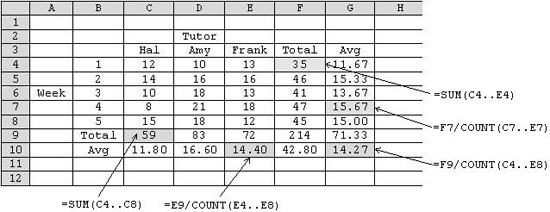
\includegraphics[scale=0.65]{xls_example.png}
\label{xls_example}
\end{figure}

电子数据表公式(通过列标号和行标号)引用了特定的单元格。在计算公式时,将用所引用的单元格中的值计算结果。每当电子数据表有变化,其中的公式都会被重新计算,所以表中的数据总是最新的。电子数据表是动态的,能对变化立即作出响应。

电子数据表中的公式可以利用标准符号(\verb|+、-、*、/|等)的基本数学运算,也可以使用电子制表软件内置的可用于公式的电子数据表函数(Spreadsheet Function)。

由于函数通常作用于一系列连续的单元格,因此电子制表软件提供了一种便捷的方式,即指定单元格的范围(range)。从语法上来讲,范围是由两个圆点及两端加两个单元格标号构成的。一个范围可以是一行中的一组单元格,如C4..E4,也可以是一列中的一组单元格,如C4..C8。此外,范围还可以是一个矩形块,指定了左上角的单元格标号和右下角的单元格标号,如C4..E8矩形块中包括了单元格C4到C8,D4到D8,E4到E8。总的来说,范围是用端点指定的一组连续单元格。

设计公式时,重要的一点是,除非特别适合,否则尽量避免在公式中使用常量。电子数据表中的原始数据发生变化,其中公式的值就会变化,公式自身也应该对插入和删除操作作出类似的响应。

电子制表软件通常会提供大量的函数。一些函数执行的是数学或统计运算、一般的金融计算或者是文本或日期的特殊运算。另一些函数则允许用户建立单元格间的逻辑关系。下表列出了一些常见的电子数据表函数。

\zihao{6}

\begin{table}[!h]
\begin{tabular}{|l|l|}
\hline
函数				&计算\\
\hline
SUM(val1,val2,...) 
\newline SUM(range)&指定的一组值的和\\
\hline
COUNT(val1,val2,...)
\newline COUNT(range)&非空单元格的个数\\
\hline
MAX(val1,val2,...)
\newline MAX(range)&指定的一组值中的最大值\\
hline
SIN(angle)	&指定角度的正弦值\\
\hline
PI()			&$\pi$的值\\
\hline
STDEV(val1,val2,...)
\newline STDEV(range)&指定的采样值的标准差\\
\hline
TODAY()	&今天的日期\\
\hline
LEFT(text,num\_chars)&指定文本的最左边的字符\\
\hline
IF(test,true\_val,false\_val)&如果test是true,则返回true\_val,否则返回false\_val\\
\hline
ISBLANK(value)&如果指定的值引用的是一个空单元格,则返回true\\
\hline
\end{tabular}
\end{table}

\zihao{5}


电子数据表的另一灵活之处是能够整行或整列地复制值或公式。复制公式时,单元格间的关系都将维持不变,因此很容易设置一整套类似的计算。在复制的公式中,对单元格的引用会被自动更新,以反映新的公式所在的行。



\section{循环引用}


电子数据表的公式可以有循环引用(Circular Reference),在计算结果时要错误地彼此依赖的一组公式,因而这种引用是不可能解决的,原因在于一个公式的结果始终是基于另一个公式的,反之亦然。例如,如果单元格B15中的公式如下:$$=\text{D22}+\text{D23}$$


而单元格D22中的公式是:$=\text{B15}+\text{B16}$

这就是一个循环引用。B15的结果要使用D22的值,而D22的结果又是由B15决定的。

循环引用通常不会这么明显,可能会涉及到多个单元格。下图展示了一个更复杂的情况,最终单元格A1的结果是由D13决定的,反之亦然。电子制表软件通常能探测出这些问题并提示错误信息。

\begin{table}[!h]
\centering
\begin{tabular}{|p{100pt}|p{200pt}|}
\hline
单元格	&内容\\
\hline
A1		&=B7*COUNT(F8..K8)\\
\hline
B7		&=A14+SUM(E40..E50)\\
\hline
E45		&=G18+G19-D13\\
\hline
D13	&=D12/A1\\
\hline
\end{tabular}
\end{table}


\section{电子数据表分析}


电子数据表的多功能性表现在用户可以决定其中的数据表示什么以及数据间的关系,因此电子数据表分析可以应用于任何领域,包括:

\begin{compactitem}
\item 跟踪销售情况
\item 分析运动统计数字
\item 维护学生的成绩单
\item 保存汽车的维修记录
\item 记录和总结旅行开销
\item 跟踪项目活动和日常安排
\item 计划股票购买
\end{compactitem}


一般说来,电子数据表的运算在商业领域的大量特定情况中是不可或缺的。

电子数据表的另一个特性是它的动态特性,一旦正确建立了电子数据表公式,那么计算会将数据的更改、添加或删除自动考虑在内。

电子数据表的动态特性还提供了进行模拟假设分析(what-if analysis)的功能。在使用中可以在电子数据表中设置一些假设,然后通过改变表示假设的值,以观察假设的变化对相关数据有什么影响,来质疑这些假设。

例如,假设我们创建了一个电子数据表用于估计举办一个研讨会的花费和潜在利润。我们可以输入参加者的人数、门票价格、资料费、会议室租金以及其他可能影响最终结果的数据,然后问自己假设分析的问题,看看随着各种条件的变化会出现哪些情况,问题如下:

\begin{compactitem}
\item 如果参加者人数减少了10\%将会怎么样?
\item 如果门票价格增加了\$5将会怎么样?
\item 如果把资料费减少一半将会怎么样?
\end{compactitem}



在问这些问题的同时改变相应的数据。如果已经正确建立了所有公式间的关系,那么每个改变都会立刻展示给我们其他数据发生了哪些变化。

商业分析师以各种方式标准化了这一过程,电子制表软件已经变成了一种主要的分析工具。成本效益分析、收支平衡计算以及预计销售价格都是通过组织电子数据表中的数据和公式来考虑适当的关系。

\chapter{数据库管理系统}


数据库(database)是一个以某种有组织的方式存储的数据集合,可以简单定义为结构化的数据集合。数据库通常是一个文件或一组文件,数据库是通过数据库管理系统(DBMS)创建和操纵的,从很大程度上说,数据库究竟是文件还是别的东西并不重要,因为我们并不直接访问数据库,数据库管理系统为我们访问数据库。

理解数据库的一个最简单的方法是将其想象为一个文件柜,此文件柜是一个存放数据的物理位置,不管数据是什么以及如何组织。

可能我们还没意识到,其实我们一直在使用数据库。当我们从电子邮件地址簿里查找名字时,或者使用搜索引擎时,都是在使用数据库。如果在工作中登录网络,也需要依靠数据库验证自己的用户名和密码。即使是在自动取款机上使用ATM卡,也要利用数据库进行PIN码验证和余额检查。

几乎所有复杂的数据库管理情况都要依靠下层的数据库和允许用户(人或程序)与之交互的支持结构。

数据库管理系统是一组软件和数据的组合,由下列几部分构成:

\begin{compactitem}
\item 物理数据库——存放数据的文件的集合;
\item 数据库引擎(engine)——支持对数据库内容的访问和修改的软件;
\item 数据库模式(schema)——存储在数据库中的数据的逻辑结构的规约。
\end{compactitem}

数据库管理系统包括存储数据的物理文件、支持数据访问和修改的软件以及指定数据库的逻辑布局的数据库模式。

数据库引擎与专用的数据库语言(比如SQL)交互,这种语言允许用户指定数据的结构,执行添加、修改、删除和更新数据的操作,以及查询数据库以获得指定的数据。

数据库模式提供了数据库中的数据的逻辑视图,独立于数据的物理存储方式。假设以一种有效的方式实现了数据库的物理结构,那么从数据库用户的观点来看,逻辑模式是更加重要的数据库视图,因为它展示了数据项之间的关系。

用户将先与数据库引擎软件交互,决定或修改数据库的模式。然后再与数据库引擎交互,访问和修改存储在磁盘上的数据库的内容。

下图展示了数据库管理系统的各个组件之间的关系。

\begin{figure}[!h]
\centering
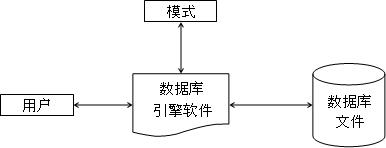
\includegraphics[scale=0.65]{db_example.png}
\label{db_example}
\end{figure}



\section{关系模型}


目前占统治地位的数据库管理模型是关系模型(Relational Model)。在关系型数据库管理系统(RDBMS)中,用表(table)组织数据项(item)和它们之间的关系(relation)。

表是记录(record)的集合。记录是域(field)的集合。数据库表的每个域都包括一个值。表中的每个记录都包含相同的域。

表中的记录又叫做数据库对象(object)或实体(entity),记录是构成一个数据库实体的相关的域的集合。记录中的域有时又叫做数据库对象的属性(attribute),是数据库记录中的一个值。

在将资料放入自己的文件柜时,并不是随便将它们扔进某个抽屉就完事了,而是在文件柜中创建文件,然后将相关的资料放入特定的文件中。在数据库领域中,这种文件就称为表。

表是一种结构化的文件,可以理解为某种特定类型的数据的结构化清单。表可以保存顾客清单、产品目录,或者其它信息清单。

这里关键的一点在于,存储在表中的数据是一种类型的数据或一个清单。绝不应该将顾客的清单与订单的清单存储在同一个数据库表中。这样做将使以后的检索和访问很困难。应该创建两个表,每个清单一个表。

表中的数据是按行(row)存储的,所保存的每个记录存储在自己的行内,如果将表想象为网格,网格中垂直的列为表列,水平行为表行。

例如,顾客表可以每行存储一个顾客,表中的行编号为记录的编号。

在很大程度上,行(row)和记录(record)这两个术语是可以互相交换使用的,但从技术上说,行才是正确的术语,行是表中的一个记录。

对记录对应,记录的域——列(column)组成了表,列中存储着表中某部分的信息,所有的表都是由一个或多个列组成的。

理解列的最好办法就是将数据库表想象为一个网格,网格中每一列存储着一条特定的信息。例如,在顾客表中,一个列存储着顾客编号,另一个列存储着顾客名,而地址、城市、州(或省)以及邮政编码全都存储在各自的列中。




\section{分解数据}


正确地将数据分解为多个列极为重要。例如,城市、州(或省)、邮政编码应该总是独立的列。通过把它分解开,才有可能利用特定的列对数据进行分类和过滤(如,找出特定州或省或特定城市的所有顾客)。如果城市和州(或省)组合在一个列中,则按州(或省)进行分类或过滤就会很困难。

数据库中每个列都有相应的数据类型(datatype),例如,如果列中存储的是数字,则相应的数据类型应该为数值类型。如果列中存储的是日期、文本、注释、金额等,则应该用恰当的数据类型规定出来。

数据类型定义(或限制)列可以存储的数据种类,例如,防止在数值字段中录入字符值等。数据类型还帮助正确地分类数据,并在优化磁盘使用方面起重要的作用。

数据类型及其名称是SQL不兼容的一个主要原因,虽然大多数数据类型得到一致的支持,但许多更为高级的数据类型却存在很大差异,甚至相同的数据类型在不同的DBMS中具有不同的名字,对此必须在创建表结构时记住这些差异。

数据库中的每个表都有一个用来标识自己的名字,此名字是唯一的。使表名成为唯一的,实际上是数据库名和表名等因素的组合,有的数据库还使用数据库拥有者的名字作为唯一名的组成部分。这表示,虽然在相同数据库中不能两次使用相同的表名,但在不同的数据库中却可以使用相同的表名。

考虑如下的数据库表,其中包含的是有关电影的信息。表中的每一行对应一条记录。表中的每条记录由相同的域构成,其中存储了特定的值。也就是说,每条电影记录都包括MovieId域、Title域、Genre域和Rating域,存放了这条记录特有的数据。数据库表都有一个名字,在这里的数据库表名是Movie。



\begin{figure}[!h]
\centering
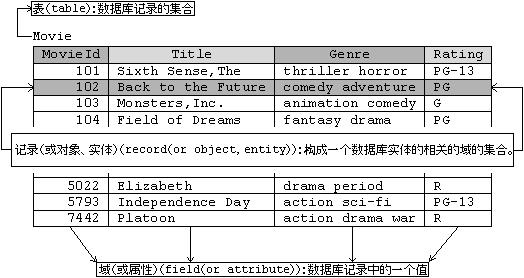
\includegraphics[scale=0.65]{table_example.png}
\label{table_example}
\end{figure}


通常,表中会有一个或多个域被标识为键(key)域\footnote{注:全国科学技术名词审定委员会审定的key在数据库中的对应名词为“键码”或“码”,不过对于key约定俗成的翻译是“键”。}。键域在表的所有记录中唯一标识了这个记录。也就是说,存储在表的每条记录的键域中的值必须是唯一的。在Movie表中,MovieId域是键的合理选择,因为两部电影可能重名,Genre域和Rating域也不适合作为键域。一般定义键(key)是在表的所有记录中唯一标识一个数据库记录的一个或多个域。


\section{主键}

唯一标识表中每行的这个列(或这组列)称为主键(Primary Key),主键用来表示一个特定的行。

没有主键,更新或删除表中特定行很困难,因为没有安全的方法保证只涉及相关的行,应该总是定义主键。

键域中的每个值都必须是唯一的,大多数DBMS可以自动生成这种域,以确保实体的唯一性。不过这并不要求键值是连续的。一个顾客表可以将顾客编号用于此目的,而包含订单的标可以使用订单ID,雇员表可以使用雇员ID或雇员社会保险号,同样地,上述Movie表中的最后三个实体包含的是截然不同的电影标识编号,只要它们是唯一的,MovieId域就可以作为域。

表中任何列都可以作为主键,只要它满足以下条件:

\begin{compactenum}
\item 任意两行都不具有相同的主键值;
\item 每个行都必须具有一个主键值(主键列不允许NULL值);
\item 主键列中的值不允许修改或更新;
\item 主键值不能重用(如果某行从表中删除,它的主键不能赋给以后的新行)。
\end{compactenum}

主键通常定义在表的一列上,但这并不是必需的,也可以一起使用多个列作为主键。在使用多个列作为主键时,上述条件必须应用到构成主键的所有列,所有列值的组合必须是唯一的(但单个列的值可以不唯一)。

另外还有一种非常重要的键,称为外键(Foreign Key)。

可以按照不同的方式排列数据库表中的记录。数据库表中的记录之间一般没有任何的内在关系。关系数据库表只是数据的逻辑视图,与底层的物理组织(记录是如何存储在存储器上)毫无关系。只有在查询数据库时,记录的排序才比较重要。例如要查询所有Rating是PG的电影,这时才可能会根据需要对查询的结果排序。

表具有一些特性,这些特性定义了数据在表中如何存储,如可以存储什么样的数据,数据如何分解,各部分信息如何命名等。描述表的这组信息就是所谓的模式(Schema),模式可以用来描述数据库中特定的表以及整个数据库(和其中表的关系)。
	
表的结构反映了它所表示的模式,也就是说,模式是表中的记录的属性的表达式。可以用下面的表达式表示上述数据库的模式:

\begin{lstlisting}[language=SQL]
Movie(MovieId : key,Title,Genre,Rating)
\end{lstlisting}
	
在模式表示法中还会说明每个域存储的数据的类型,如数字或文本等。此外还可能说明某个域可用的值的集合。例如在上述的数据库表中,可以说明Rating域的值只能是G、PG、PG-13、R或NC-17。整个数据库的模式由其中每个表的模式构成。

假设我们要创建一项电影租赁业务。除了出租的电影的清单外,还要创建一个客户信息表,我们使用Customer表存放了客户的信息。

\begin{figure}[!h]
\centering
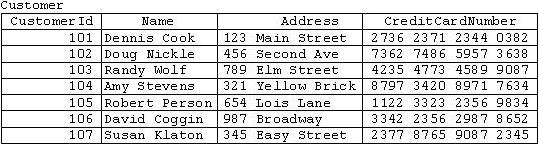
\includegraphics[scale=0.5]{table_customer.png}
\label{table_customer}
\end{figure}

与Movie表一样,Customer表也有一个键CustomerId域。某些CustomerId的值与MovieId的值相同,它们不会冲突。键的值只需要在同一个表中是唯一的。


正确地将数据分解为多个列极为重要,例如,城市、周、邮政编码应该总是独立的列。在真实的数据库中,最好把Name域分为FirstName和LastName两个域。此外,完整的地址也可能会根据实际情况的需要被分为几个部分,如City和State。通过分解数据才有可能利用特定的列对数据进行分类和过滤(例如,找出特定州或省或特定城市的所有顾客)。


Movie表和Customer表说明了如何用独立的表中的记录组织数据。而关系数据库管理系统的强大之处在于创建能把各个表从概念上联系起来的表,也就是说,数据库元素之间的关系可以用新的表表示,这个表也可以有自己的属性。

关系表并不是重复其他表的数据,而是存储数据库记录的关键值,以便需要的时候能够查找详细的数据。

%%
%%
%%
%%
%%
%%
%%
%%
\section{关系}


根据关系模型中的定义,记录表示的是独立的数据库对象,记录的域是这些对象的属性。可以创建一个记录来表示对象之间的关系,包括记录中的属性之间的关系。因此,可以用一个表来表示对象间的关系的集合。


继续深化上述电影出租的例子,要表示特定的客户租了哪些电影。由于“租用”是客户和电影之间的关系,所以可以把它表示为一个记录。租用的日期和到期日是这种关系的属性,于是可以创建一个新的数据库表Rents来表示当前被租走的电影的关系记录的集合。



\begin{figure}[!h]
\centering
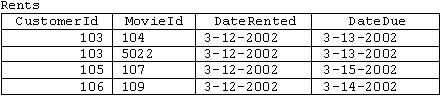
\includegraphics[scale=0.5]{table_rents.png}
\label{table_rents}
\end{figure}


Rents表包含有关关系中的对象(客户和电影)的信息和关系的属性。但是要注意的是,它并非包含客户和电影的所有信息。

在关系数据库中要尽量避免数据重复。例如,在Rents表中没有必要保存客户的名字和地址。Customer表已经存储了这些数据。当需要这些数据时,用存储在Rents表中的CustomerId来检索Customer表,查找该客户的详细信息即可。同样地,当需要有关电影的信息时,用MovieId检索Movie表即可。


在上述的Rents表中,CustomerId的值中出现了两次103,这说明同一个客户可以租借至少两部电影。


数据库表中的数据会根据需要被修改、添加、更新和删除。当给库存添加了电影或从中删除了电影时,Movie表中的记录都要更新。当有新客户的记录加入时,需要把它们添加到Customer表中。随着电影不断地被租出去或归还回来,还要添加或删除Rents表中的记录。


	
%%
%%
%%
%%
%%
%%
%%
%%
\section{通用产品代码}

使用通用产品代码(UPC)和与之关联的条形码是为了加速顾客在商店购买产品的速度,以及帮助跟踪库存。

\begin{figure}[!h]
\centering
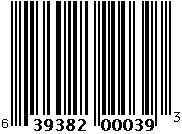
\includegraphics[scale=0.5]{universal_product_code.png}
\label{universal_product_code}
\end{figure}


UPC符号由机器能识别的条形码和人能识别的12位UPC编号组成。UPC编号的前6位数字是制造商的身份编号,接下来的5位数字是项目编号。每种类型的产品与同一产品的不同包装都有一个唯一的项目编号。因此,两升装的可口可乐和两升装的减肥可乐项目编号不同。最后一位UPC代码叫做校验数位,扫描器可以用它来确定扫描的UPC编号是否正确。校验数位是通过对UPC编号的其余数位的计算得来的。在读入UPC编号后,扫描器将对它执行运算,用校验数位进行验证。

针对某些产品,尤其是小产品,开发了新的UPC编号法,通过减少某些数位从而缩减了UPC编号。采用这种方法,可以减小整个UPC符号的大小。

注意,UPC编号并不存储产品的价格。当收银机(或者电子收款系统,POS)扫描一个产品时,它将使用UPC编号中的制造商编号和项目编号在数据库中检索该项目,而数据库则包含大量的产品信息,包括它的价格等。UPC中只保留基本的信息,这样不必更改产品的标签,就可以很容易的更改其他信息(比如价格等)。


%%
%%
%%
%%
%%
%%
%%
%%
%%
%%
%%
%%
%%
%%

\chapter{结构化查询语言}


结构化查询语言(Structured Query Language,SQL)是一种用于管理关系数据库的综合性数据库语言,包括指定数据库模式的语句和添加、修改、更新和删除数据库内容的语句。另外,还具有查询数据库以获取特定数据的功能。

SQL的原始版本是20世纪70年代IBM开发的Sequal语言。设计SQL的目的是很好地完成一项任务——提供一种从数据库中读写数据的简单有效的方法。

1986年,美国国家标准化组织(ANSI)发布了SQL标准,这是访问关系数据库的商用数据库语言的基础。

SQL有如下的优点:

\begin{compactitem}
\item SQL不区分大小写,空格被用作语句中的分隔符。
\item SQL不是某一个特定数据库专有的语言,几乎所有重要的DBMS都支持SQL。
\item SQL的语句全都是由有很强描述性的英语单词组成的。
\end{compactitem}

大多数DBMS以不自己完成文件分布的格式存储数据,这些SQL依赖于具体的DBMS运行。

许多DBMS提供商通过增加语句或指令,对SQL进行了扩展,这种扩展的目的是提供执行特定操作的额外功能或简化方法,虽然这种扩展很有用,但一般都是针对个别DBMS的,很少有两个以上的提供商支持这种扩展。

所有主要的DBMS,即使有自己的扩展,但这些扩展都支持ANSI SQL,比如PL/SQL、Transact-SQL等,其中PL/SQL是Oracle公司为其数据库产品开发的SQL扩展,Transact-SQL是微软与Sybase公司合作开发,适用于微软SQL Server和Sybase数据库。
%%
%%
%%
%%
%%
\section{ODBC}


ODBC(Open Database Connectivity)是一个为访问数据库提供的标准C接口,于1992年由SQL Access Group标准化,定义了一组用于访问数据库的标准C API。ODBC作为应用程序和数据库之间的中间件,使应用程序能与不同的后端数据库或基础数据库引擎交互。

ODBC本身不是数据库。但ODBC包装数据库,使所有数据库以一种一致和清晰定义的方式工作。它利用具有两种主要功能的软件驱动程序达到这一点。首先,它们封装数据库的本身特性或特色并对客户机隐藏它们。其次,它们提供一种常用的语言与这些数据库交互(在需要时进行转换)。ODB所用的语言就是SQL。

ODBC客户机应用程序并不直接与数据库交互,而是与ODBC数据源交互。数据源是一个逻辑数据库,它包括驱动程序(每种类型的数据库有自己的驱动程序)和如何连接到数据库的信息(文件路径、服务器名等)。

在定义了数据库源后,任何兼容ODBC的应用程序都可以使用这些数据源。ODBC并不针对具体的应用程序,它们针对的是系统。存在许多不同的ODBC程序版本,因此在设置具体的ODBC数据源时,应该密切注意具体的提示。

If you are using 64-bit Windows, be sure to check the documentation for how to configure the ODBC driver.  The short answer is:

\begin{compactenum}
\item Click Start / Run
\item Type \texttt{\%windir\%{\textbackslash}SysWOW64{\textbackslash}ODBCAD32.exe}
\item Continue configuring as normal.
\end{compactenum}


%%
%%
%%
%%
%%
\section{SQL的数学基础}


SQL的操作中混有代数,用于访问和操作关系表中的数据。这种代数是20世纪60年代末期由IBM的E.F.Codd定义的。SQL的基本操作包括:

\begin{compactitem}
\item select操作,用于识别表中的记录。
\item project操作,用于生成表列的子集。
\item 笛卡尔乘积操作,用于连接两个表的行。
\end{compactitem}

其他还有集合操作联合、求差、求交集、自然连接(笛卡尔乘积的子集)和除法操作。

编写SQL语句需要对基本的数据库设计有良好的理解。不知道什么信息存放在什么表中,表与表之间如何互相关联,以及行中数据如何分解,要编写高效的SQL是不可能的。

下面所用的表为一个假想的玩具销售商使用的订单录入系统的组成部分。这些表用来完成几项任务:

\begin{compactitem}
\item 管理供应商;
\item 管理产品目录;
\item 管理客户列表;
\item 录入客户订单;
\end{compactitem}

完成它们需要5个表(它们作为一个关系数据库设计的组成部分紧密关联)。虽然现实世界中的订单录入系统还记录了这里没有包括的大量数据(如工资和记账信息、发货追踪信息等)。不过,这些表确实示范了现实世界中会遇到的各种数据的组织和关系。

下面对5个表及每个表内的列名进行介绍。

\begin{compactenum}
\item Vendors表

Vendors表存储卖产品的供应商。每个供应商在这个表中有一个记录,供应商ID列(vend\_id)用于产品与供应商的匹配。

\begin{longtable}{|m{180pt}|m{180pt}|}
%%head
\hline
\multicolumn{2}{|c|}{Vendors表的列}
\tabularnewline\hline
列	&说明
\endhead
%%endhead

%%firsthead
\hline
\multicolumn{2}{|c|}{Vendors表的列}
\tabularnewline\hline
列	&说明
\endfirsthead
%%endfirsthead

%%foot
\multicolumn{2}{r}{}
\endfoot
%%endfoot

%%lastfoot
\endlastfoot
%%endlastfoot
\hline
vend\_id		&唯一的供应商ID\\
\hline
vend\_name		&供应商名\\
\hline
vend\_address	&供应商的地址\\
\hline
vend\_city		&供应商的城市\\
\hline
vend\_state		&供应商的州\\
\hline
vend\_zip		&供应商的邮政编码\\
\hline
vend\_country	&供应商的国家\\
\hline

\end{longtable}

所有表都应该有主键,这个表应该用vend\_id作为它的主键。

\item Products表

Products表包含产品目录,每行一个产品。每个产品有唯一的ID(prod\_id列),并且借助vend\_id(供应商的唯一ID)与供应商相关联。



\begin{longtable}{|m{180pt}|m{180pt}|}
%%head
\hline
\multicolumn{2}{|c|}{Products表的列}
\tabularnewline\hline
列	&说明
\endhead
%%endhead

%%firsthead
\hline
\multicolumn{2}{|c|}{Products表的列}
\tabularnewline\hline
列	&说明
\endfirsthead
%%endfirsthead

%%foot
\multicolumn{2}{r}{}
\endfoot
%%endfoot

%%lastfoot
\endlastfoot
%%endlastfoot
\hline
prod\_id		&唯一的产品ID\\
\hline
vend\_id		&产品供应商ID(关联到Vendors表的vend\_id列\\
\hline
prod\_name		&产品名\\
\hline
prod\_price		&产品价格\\
\hline
prod\_desc		&产品描述\\
\hline

\end{longtable}

所有表都应该有主键,这个表应该用prod\_id作为它的主键。

为实施引用完整性,应该在vend\_id上定义一个外键,关联它到Vendors的vend\_id列。

\item Customers表

Customers表存储所有客户信息。每个客户有唯一的ID(cust\_id列)。

\begin{longtable}{|m{180pt}|m{180pt}|}
%%head
\hline
\multicolumn{2}{|c|}{Customers表的列}
\tabularnewline\hline
列	&说明
\endhead
%%endhead

%%firsthead
\hline
\multicolumn{2}{|c|}{Customers表的列}
\tabularnewline\hline
列	&说明
\endfirsthead
%%endfirsthead

%%foot
\multicolumn{2}{r}{}
\endfoot
%%endfoot

%%lastfoot
\endlastfoot
%%endlastfoot
\hline
cust\_id		&唯一的客户ID\\
\hline
cust\_name	&客户名\\
\hline
cust\_address&客户的地址\\
\hline
cust\_city	&客户的城市\\
\hline
cust\_state	&客户的州\\
\hline
cust\_zip	&客户的邮政编码\\
\hline
cust\_country&客户的国家\\
\hline
cust\_contact&客户的联系名\\
\hline
cust\_email	&客户的联系电子邮件地址\\
\hline

\end{longtable}

所有表都应该有主键,这个表应该用cust\_id作为它的主键。

\item Orders表

Orders表存储客户订单(但不是订单细节)。每个订单唯一地进行编号(order\_num列)。Orders表按cust\_id列(关联到Customers表的客户唯一ID)关联到相应的客户。


\begin{longtable}{|m{180pt}|m{180pt}|}
%%head
\hline
\multicolumn{2}{|c|}{Orders表的列}
\tabularnewline\hline
列	&说明
\endhead
%%endhead

%%firsthead
\hline
\multicolumn{2}{|c|}{Orders表的列}
\tabularnewline\hline
列	&说明
\endfirsthead
%%endfirsthead

%%foot
\multicolumn{2}{r}{}
\endfoot
%%endfoot

%%lastfoot
\endlastfoot
%%endlastfoot
\hline
order\_num	&唯一的订单号\\
\hline
order\_date	&订单日期\\
\hline
cust\_id		&订单客户ID(关联到Customers表的cust\_id)\\
\hline
\end{longtable}

所有表都应该有主键。这个表应该用order\_num作为它的主键。

为实施引用完整性,应该在cust\_id上定义一个外键,关联它到Customers表的cust\_id列。

\item OrderItems表

OrderItems表存储每个订单中的实际物品,每个订单的每个物品一行。对于Orders表中的每一行,在OrderItems表中有一行或多行。每个订单物品由订单号加订单物品(第一个物品、第二个物品等)唯一标识。订单物品用order\_num列(关联到Orders表中订单的唯一ID)与其对应的订单相关联。此外,每个订单物品包含该物品的产品ID(把物品关联到Products表)。


\begin{longtable}{|m{180pt}|m{180pt}|}
%%head
\hline
\multicolumn{2}{|c|}{OrderItems表的列}
\tabularnewline\hline
列	&说明
\endhead
%%endhead

%%firsthead
\hline
\multicolumn{2}{|c|}{OrderItems表的列}
\tabularnewline\hline
列	&说明
\endfirsthead
%%endfirsthead

%%foot
\multicolumn{2}{r}{}
\endfoot
%%endfoot

%%lastfoot
\endlastfoot
%%endlastfoot
\hline
order\_num	&订单号(关联到Orders表的order\_num)\\
\hline
order\_item	&订单物品号(订单内的顺序)\\
\hline
prod\_id	&产品ID(关联到Products表的prod\_id)\\
\hline
quantity	&物品数量\\
\hline
item\_price	&物品价格\\
\hline

\end{longtable}

所有表都应该有主键。这个表应该用order\_num和order\_item作为它的主键。

为实施引用完整性,应该在order\_num和prod\_id上定义外键,关联order\_num到Orders的order\_num列,关联prod\_id到Products表的prod\_id列。

\end{compactenum}
%%
%%
%%
%%
%%
%%


\section{SQL数据类型}

SQL中数据类型是定义列中可以存储什么数据以及该数据实际怎样存储的基本规则。数据类型用于以下目的:

\begin{compactitem}
\item 数据类型允许限制可存储在列中的数据。例如,数值数据类型列只能接受数值。
\item 数据类型允许在内部更有效地存储数据。例如,可以用一种比文本串更简洁的格式存储数值和日期时间值。
\item 数据类型允许变换排序顺序。如果所有数据都作为串处理,则1位于10之前,而10又位于2之前(串以字典顺序排序,从左边开始比较,一次一个字符)。作为数值数据类型,数值才能正确排序。
\end{compactitem}

在设计表时,应该特别重视所用的数据类型。使用错误的数据类型可能会严重地影响应用程序的功能和性能。更改包含数据的列不是一件小事(而且这样做可能会导致数据丢失)。

任意两个DBMS都不是完全相同的,不同DBMS的数据类型可能有很大的不同。在不同的DBMS中,即使具有相同名称的数据类型也可能代表不同的东西。

\subsection{串数据类型}

最常用的数据类型是串数据类型。它们存储串,如名字、地址、电话号码、邮政编码等。有两种基本的串类型,分别为:定长串和变长串。

定长串接受长度固定的字符串,其长度是在创建表时指定的。例如,名字列可允许30个字符,而社会安全号列允许11个字符(允许的字符数目中包括两个破折号)。定长列不允许多于指定的字符数目。它们分配的存储空间和指定的一样多。因此,如果串Ben存储到30个字符的名字字段,则存储的是30个字符,缺少的字符用空格填充,或根据需要补为NULL。

变长串存储任意长度的文本(其最大长度随不同的数据类型和DBMS而变化)。有些变长数据类型具有最小的定长,而有些则是完全变长的。不管是哪种,只有指定的数据得到保存(额外的数据不保存)。

串数据类型分为定长串和变长串,有一个原因是出于性能的考虑。DBMS处理定长列远比处理变长列快得多。此外,许多DBMS不允许对变长列(或一个列的可变部分)进行索引。这也会极大地影响性能。

\begin{longtable}{|m{200pt}|m{180pt}|}
%%head
\hline
\multicolumn{2}{r}{}
\tabularnewline\hline
\endhead
%%endhead

%%firsthead
\caption{串数据类型}\\
\hline
\endfirsthead
%%endfirsthead

%%foot
\multicolumn{2}{r}{}
\endfoot
%%endfoot

%%lastfoot
\endlastfoot
%%endlastfoot
\hline
CHAR	&1~255个字符的定长串。它的长度必须在创建时规定。\\
\hline
NCHAR	&CHAR的特殊形式,用来支持多字节或Unicode字符(此类型的不同实现变化很大)\\
\hline
NVARCHAR&TEXT的特殊形式,用来支持多字节或Unicode字符(此类型的不同实现变化很大)\\
\hline
TEXT(也称为LONG,MEMO或VARCHAR)&变长文本\\
\hline
\end{longtable}

不管使用何种形式的串数据类型,串值都必须括在单引号内。

另外,当数值不是数值时,比如电话号码和邮政编码等,此时需要遵守的基本规则是:如果数值是计算(求和、平均等)中使用的数值,则应该存储在数值数据类型列中。如果作为字符串(可能包含数字)使用,则应该保存在串数据类型列中。

\subsection{数值数据类型}


数值数据类型存储数值。多数DBMS支持多种数值数据类型,每种存储的数值具有不同的取值范围。显然,支持的取值范围越大,所需存储空间越多。此外,有的数值数据类型支持使用十进制小数点(和小数),而有的则只支持整数。并非所有的DBMS都支持下列所列出的数值数据类型名称约定和描述。


\begin{longtable}{|m{180pt}|m{180pt}|}
%%head
\hline
\multicolumn{2}{r}{}
\tabularnewline\hline
\endhead
%%endhead

%%firsthead
\caption{数值数据类型}\\
\hline
\endfirsthead
%%endfirsthead

%%foot
\multicolumn{2}{r}{}
\endfoot
%%endfoot

%%lastfoot
\endlastfoot
%%endlastfoot
\hline
BIT 		&单个二进制位值,或者为0或者为1,主要用于开/关标志。\\
\hline
DECIMAL(或NUMERIC)&定点或精度可变的浮点值\\
\hline
FLOAT(或NUMERIC)&浮点值\\
\hline
INT(或INTEGER)&4字节整数值,支持从-2147483648~2147483647的数\\
\hline
REAL&4字节浮点值\\
\hline
SMALLINT&2字节整数值,支持从-32768~32767的数\\
\hline
TINYINT&1字节整数值,支持从0~255的数\\
\hline
\end{longtable}

与串数据类型不一样,数值不应该括在引号内。

多数DBMS支持一种用来存储货币值的特殊数值数据类型。一般记为MONEY或CURRENCY,这种数据类型基本上是特定取值范围的DECIMAL数据类型,只不过更适合存储货币值。

\subsection{日期和时间数据类型}

所有DBMS都支持用来存储日期和时间值的数据类型。与数值一样,多数DBMS都支持多种这种类型,每种具有不同的取值范围和精度。

\begin{longtable}{|m{180pt}|m{180pt}|}
%%head
\hline
\multicolumn{2}{r}{}
\tabularnewline\hline
\endhead
%%endhead

%%firsthead
\caption{日期和时间数据类型}\\
\hline
\endfirsthead
%%endfirsthead

%%foot
\multicolumn{2}{r}{}
\endfoot
%%endfoot

%%lastfoot
\endlastfoot
%%endlastfoot
\hline
DATE	&日期值\\
\hline
DATETIME(或TIMESTAMP)&日期时间值\\
\hline
SMALLDATETIME&日期时间值,精确到分(无秒或毫秒)\\
\hline
TIME&时间值\\
\hline
\end{longtable}

没有所有DBMS都理解的定义日期的标准方法。多数实现都理解诸如2004-12-30或Dec 30th,2004等格式,但即使这样,有的DBMS还是不理解它们。


\subsection{ODBC日期}


因为每种DBMS都有自己特定的日期格式,所以ODBC创建了自己的一种格式。在ODBC被使用时对每种数据库都起作用。

ODBC格式对于日期类似于\{d ‘2004-12-30’\},对于时间类似于\{t ‘21:46:29’\},而对于日期时间类似于\{ts ‘2004-12-30 21:46:29’\}。如果通过ODBC使用SQL,应该以这种方式格式化日期和时间。


\subsection{二进制数据类型}

二进制数据类型是最不具有兼容性的数据类型。与其他所有数据类型(它们具有特定的用途)不一样,二进制数据类型可包含任何数据,包括二进制信息,如图像、多媒体、字处理文档等。

\begin{longtable}{|m{180pt}|m{180pt}|}
%%head
\hline
\multicolumn{2}{r}{}
\tabularnewline\hline
\endhead
%%endhead

%%firsthead
\caption{二进制数据类型}\\
\hline
\endfirsthead
%%endfirsthead

%%foot
\multicolumn{2}{r}{}
\endfoot
%%endfoot

%%lastfoot
\endlastfoot
%%endlastfoot
\hline
BINARY	&定长二进制数据(最大长度从255字节到8000字节,有赖于具体的实现)\\
\hline
LONG RAW&变长二进制数据,最大2GB\\
\hline
RAW(某些实现为BINARY)&定长二进制数据,最多255字节\\
\hline
VARBINARY&变长二进制数据(最大长度一般在255字节到8000字节间变化,依赖于具体的实现)\\
\hline
\end{longtable}



\section{SQL保留字}

SQL是由关键字组成的语言,关键字是一些用于执行SQL操作的特殊词汇。在命名数据库、表、列和其他数据库对象时,一定不要使用这些关键字。因此,关键字是一定要保留的。下面列出的是主要的DBMS中最常用的保留字。

\begin{compactitem}
\item 关键字随不同的DBMS而变化,并非所列出的关键字都被所有DBMS采用;
\item 许多DBMS扩展了SQL保留字,使其包含专门用于实现的术语。多数DBMS专用的关键字未列出;
\item 为保证以后的兼容性和可移植性,应避免使用这些可能的保留字,即使它们不是当前使用的DBMS的保留字也是如此。
\end{compactitem}

\begin{longtable}{m{120pt}m{120pt}m{120pt}}
\rowcolors{1}{White}{Lavender}
%%head
\endhead
%%endhead

%%firsthead
\caption{SQL保留字}\\
\endfirsthead
%%endfirsthead

%%foot
\endfoot
%%endfoot

%%lastfoot
\endlastfoot
%%endlastfoot
ABORT						&ABSOLUTE		&	ACTION					\\
ACTIVE						&ADD				&AFTER\\
ALL							&ALLOCATE		&	ALTER\\
ANALYZE					&AND				&ANY\\
ARE							&AS				&	ASC\\
ASCENDING					&ASSERTION		&	AT\\
AUTHORIZATION			&AUTO				&AUTO-INCREMENT\\
AUTOING					&AVG				&BACKUP\\
SEFORE						&BEGIN				&BETWEEN\\
BIGINT						&BINARY			&	BIT\\
BLOB						&BOOLEAN			&BOTH\\
BREAK						&BROWSE			&BULK\\
BY							&BYTES				&CACHE\\
CALL						&CASCADE			&CASCADED\\
CASE						&CAST				&CATALOG\\
CHANGE					&CHAR				&CHARACTER\\
CHARACTER\_LENGTH		&CHECK			&	CHECKPOINT\\
CLOSE						&CLUSTER			&CLUSTERED\\
COALESCE					&COLLATE			&COLUMN\\
COLUMNS					&COMMENT		&	COMMIT\\
COMMITTED				&COMPUTE			&COPUTED\\
CONDITIONAL				&CONFIRM			&CONNECT\\
CONNECTION				&CONSTRAINT		&CONSTRAINS\\
CONTAINING				&CONTAINS		&	CONTAINSTABLE\\
CONTINUE					&CONTROROW		&CONVERT\\
COPY						&COUNT			&	CREATE\\
CROSS						&CSTRING			&CUBE\\
CURRENT					&CURRENT\_DATE	&CURRENT\_TIME\\
CURRENT\_TIMESTAMP		&CURRENT\_USER	&CURSOR\\
DATABASE					&DATABASES		&	DATE\\
DATETIME					&DAY				&DBCC\\
DEALLOCATE				&DEBUG			&	DEC\\
DECIMAL					&DECLARE			&DEFAULT\\
DELETE						&DENY				&DESC\\
DESCENDING				&DESCRIBE			&DISCONNECT\\
DISK						&DISTINCT			&DISTRIBUTED\\
DIV							&DO				&	DOMAIN\\
DOUBLE					&DROP				&DUMMY\\
DUMP						&ELSE				&ELSEIF\\
ENCLOSED					&END				&ERRLVL\\
ERROREXIT					&ESCAPE			&	ESCAPED\\
EXCEPT						&EXCEPTION		&	EXEC\\
EXECUTE					&EXISTS			&	EXIT\\
EXPLAIN					&EXTEND			&EXTERNAL\\
EXTRACT					&FALSE				&FETCH\\
FIELD						&FIELDS			&	FILE\\
FILLFACTOR					&FILTER			&	FLOAT\\
FLOPPY						&FOR				&FORCE\\
FOREIGN					&FOUND			&	FREETEXT\\
FREETEXTTABLE				&FROM				&FULL\\
FUNCTION					&GENERATOR		&GET\\
GLOBAL					&GO				&	GOTO\\
GRANT						&GROUP			&	HAVING\\
HOLDLOCK					&HOUR				&IDENTITY\\
IF							&IN					&INACTIVE\\
INDEX						&INDICATOR		&	INFILE\\
INNER						&INOUT			&	INPUT\\
INSENSITIVE				&INSERT			&	INT\\
INTEGER					&INTERSECT		&	INTERVAL\\
INTO						&IS					&ISOLATION\\
JOIN						&KEY				&	KILL\\
LANGUAGE					&LAST				&LEADING\\
LEFT						&LENGTH			&LEVEL\\
LIKE						&LIMIT				&LINENO\\
LINES						&LISTEN			&	LOAD\\
LOCAL						&LOCK				&LOGFILE\\
LONG						&LOWER			&	MANUAL\\
MATCH						&MAX				&MERGE\\
MESSAGE					&MIN				&MINUTE\\
MIRROREXIT					&MODULE			&MONEY\\
MONTH						&MOVE				&NAMES\\
NATIONAL					&NATUAL			&NCHAR\\
NEXT						&NEW				&NO\\
NOCHECK					&NONCLUSTERED	&NONE\\
NOT						&NULL				&NULLIF\\
NUMERIC					&OF				&	OFF\\
OFFSET						&OFFSETS			&ON\\
ONCE						&ONLY				&OPEN\\
OPTION						&OR				&	ORDER\\
OUTER						&OUTPUT			&OVER\\
OVERFLOW					&OVERLAPS		&	PAD\\
PAGE						&PAGES			&	PARAMETER\\
PARTIAL					&PASSWORD		&	PERCENT\\
PERM						&PERMANENT		&PIPE\\
PLAN						&POSITION			&PRECISION\\
PREPARE					&PRIMARY			&PRINT\\
PRIOR						&PRIVILEGES		&	PROC\\
PROCEDURE				&PROCESSEXIT		&PROTECTED\\
PUBLIC						&PURGE			&	PAISERROR\\
READ						&READEXIT			&REAL\\
REFERENCES				&REGEXP			&RELATIVE\\
RENAME					&REPEAT			&	REPLACE\\
REPLICATION				&REQUIRE			&RESERV\\
RESERVING					&RESET				&RESTORE\\
RESTRICT					&RETAIN			&	RETURN\\
RETURNS					&REVOKE			&RIGHT\\
ROOLBACK					&ROLLUP			&ROWCOUNT\\
RULE						&SAVE				&SAVEPOINT\\
SCHEMA					&SECOND			&SECTION\\
SEGMENT					&SELECT			&	SENSITIVE\\
SEPARATOR					&SEQUENCE		&	SESSION\_USER\\
SET							&SETUSER			&SHADOW\\
SHARED					&SHOW			&	SHUTDOWN\\
SINGULAR					&SIZE				&SMALLINT\\
SNAPSHOT					&SOME				&SORT\\
SPACE						&SQL				&	SQLCODE\\
SQLERROR					&STABILITY			&STARTING\\
STARTS						&SATAISTICS		&	SUBSTRING\\
SUM						&SUSPEND			&TABLE\\
TABLES						&TAPE				&TEMP\\
TEMPORARY				&TEXT				&TEXTSIZE\\
THEN						&TIME				&TIMESTAMP\\
TO							&TOP				&	TRAILING\\
TRAN						&TRANSACTION	&	TRANSLATE\\
TRIGGER					&TRIM				&TRUE\\
TRUNCATE					&UNCOMMITTED	&	UNION\\
UNIQUE						&NUTIL				&UPDATE\\
UPDATETEXT				&UPPER			&	USAGE\\
USE							&USER				&USING\\
VALUE						&VALUES			&	VARCHAR\\
VARIABLE					&VARYING			&VERBOSE\\
VIEW						&VOLUME			&WAIT\\
WAITFOR					&WHEN			&	WHERE\\
WHILE						&WITH				&WORK\\
WRITE						&WRITETEXT		&	XOR\\
YEAR						&ZONE	&\\
\end{longtable}






\chapter{查询}


提交给数据库的信息请求称为查询(Query),select语句是查询的主要工具,它具有很多变体,能够访问数据库中的特定数据。

基本的select语句包括一个select从句、一个from从句和一个where从句。

\begin{lstlisting}[language=SQL]
select attribute-list from table-list where condition
\end{lstlisting}

select从句决定了要返回那些属性。from从句决定了使用哪个表进行查询。where从句限制了返回的数据。例如:

\begin{lstlisting}[language=SQL]
select Title from Movie where Rating = 'PG'
\end{lstlisting}

这个查询的结果是Movie表中所有Rating为PG的电影名的列表。如果不需要特殊的限制,可以省略where从句:

\begin{lstlisting}[language=SQL]
select Name,Address from Customer
\end{lstlisting}

这个查询返回的是Customer表中所有客户的名字和地址。select从句中的星号(*)表示要返回选中的记录中的所有属性:

\begin{lstlisting}[language=SQL]
select * from Movie where Genre like '%action%'
\end{lstlisting}

这个查询返回的是Movie表中Genre属性包含单词action的记录的所有属性。SQL中的like操作执行的是字符串的模式匹配,符号\%与任何字符串都匹配。

select语句还可以用order从句指定查询结果的排序方法:

\begin{lstlisting}[language=SQL]
select * from Movie where Rating = 'R' order by Title
\end{lstlisting}

这个查询返回的是Rating为R的电影的所有属性,按照电影名的字母顺序排列。

SQL支持的select语句还有很多的变体,可以进一步细化查询。
%%
%%
%%
%%
%%
%%
\chapter{修改}


用SQL中的insert、update和delete语句,可以改变表中的数据,包括对数据库执行添加、修改和删除操作等。

insert语句可以给表添加一条新记录。每个insert语句都指定了新记录的属性值。例如:

\begin{lstlisting}[language=SQL]
insert into Customer values(9876,'John Smith',
'602 Greenbriar Court','2980 3423 5564 8796')
\end{lstlisting}
	
	这个语句将在Customer表中插入一条指定了属性的新记录。
	
	update语句可以改变表中的一条或多条记录的值。例如:
	
\begin{lstlisting}[language=SQL]
update Movie set Genre='thriller drama' where title='Unbreakable'
\end{lstlisting}
	
	这个语句将把电影Unbreakable的Genre属性改为thriller drama。
	
	delete语句可以删除表中与指定的条件匹配的所有记录。例如,如果要删除Movie表中所有Rating为R的电影,可以使用下列delete语句:
	
\begin{lstlisting}[language=SQL]
delete from Movie where Rating = 'R'
\end{lstlisting}

	
	与select语句一样,insert、update和delete语句也有很多变体。
%%
%%
%%
%%
%%
%%
%%
\chapter{SQL语句}

在书写SQL语句和阅读语句语法时,应该记住以下约定:

\begin{compactitem}
\item |符号用来指出几个选择中的一个,因此,NULL | NOT NULL表示或者给出NULL或者给出NOT NULL。
\item 包含在方括号中的关键词或子句(如[like this])是可选的。
\item SQL基本语句的语法几乎对所有DBMS都有效。
\end{compactitem}

\section{ALTER TABLE}

ALTER TABLE用来更新已存在的表的结构。为了创建表,应该使用CREATE TABLE。

\begin{lstlisting}[language=SQL]
ALTER TABLE
(
	ADD | DROP column datatype [NULL | NOT NULL] [CONSTRAINS],
	ADD | DROP column datatype [NULL | NOT NULL] [CONSTRAINS],
	. . .
);
\end{lstlisting}


\section{COMMIT}

COMMIT用来将事务处理写到数据库。

\begin{lstlisting}[language=SQL]
COMMIT [TRANSACTION];
\end{lstlisting}

\section{CREATE INDEX}

CREATE INDEX用于在一个或多个列上创建索引。

\begin{lstlisting}[language=SQL]
CREATE INDEX indexname 
ON tablename (column, . . . );
\end{lstlisting}

\section{CREATE PROCEDURE}

CREATE PROCEDURE用于创建存储过程。Oracle的语法稍有不同。

\begin{lstlisting}[language=SQL]
CREATE PROCEDURE procedurename [parameters] [options] 
AS SQL statement;
\end{lstlisting}


\section{CREATE TABLE}

CREATE TABLE用于创建新数据库表。为更新已经存在的表的结构,使用ALTER TABLE。

\begin{lstlisting}[language=SQL]
CREATE TABLE tablename
(
	column datatype [NULL | NOT NULL] [CONSTRAINS],
	column datatype [NULL | NOT NULL] [CONSTRAINS],
	. . .
);
\end{lstlisting}

\section{CREATE VIEW}

CREATE VIEW用来创建一个或多个表上的新视图。

\begin{lstlisting}[language=SQL]
CREATE VIEW viewname AS
SELECT columns, . . .
FROM tables, . . .
[WHERE . . .]
[ORDER BY . . .]
[HAVING . . .];
\end{lstlisting}

\section{DELETE}

DELETE从表中删除一行或多行。

\begin{lstlisting}[language=SQL]
DELETE FROM tablename
[WHERE . . .];
\end{lstlisting}

\section{DROP}

DROP永久地删除数据库对象(表、视图、索引等)。

\begin{lstlisting}[language=SQL]
DROP INDEX | PROCEDURE | TABLE | VIEW indexname | procedurename | tablename | viewname;
\end{lstlisting}

\section{INSERT}

INSERT给表增加行。

\begin{lstlisting}[language=SQL]
INSERT INTO tablename [(columns, . . .)]
VALUES(values, . . .);
\end{lstlisting}

\section{INSERT SELECT}

INSERT SELECT插入SELECT的结果到一个表。

\begin{lstlisting}[language=SQL]
INSERT INTO tablename [(columns, . . .)]
SELECT columns, . . . FROM tablename, . . .
[WHERE . . .];
\end{lstlisting}


\section{ROLLBACK}


ROLLBACK用于撤销一个事务处理块。

\begin{lstlisting}[language=SQL]
ROLLBACK [TO savepointname];
\end{lstlisting}

或者:

\begin{lstlisting}[language=SQL]
ROLLBACK TRANSACTION;
\end{lstlisting}


\section{SELECT}

SELECT用于从一个或多个表(视图)中检索数据。

\begin{lstlisting}[language=SQL]
SELECT columnname, . . .
FROM tablename, . . .
[WHERE . . .]
[UNION . . .]
[GROUP BY . . .]
[HAVING . . .]
[ORDER BY . . .];
\end{lstlisting}


\section{UPDATE}

UPDATE更新表中一行或多行。

\begin{lstlisting}[language=SQL]
UPDATE tablename
SET columnname = value, . . .
[WHERE . . .];
\end{lstlisting}
%%
%%
%%
%%
%%
%%
%%
%%
%%
%%
%%
%%
%%
%%
\chapter{SQL基本操作}

SQL是一种语言而不是应用程序,SQL语句是由简单的英语单词构成的,这些单词称为关键字,每个SQL语句都是由一个或多个关键字(keyword)构成的。

关键字是作为SQL组成部分的保留字,关键字不能用作表或列的名字。

SQL语句由子句(clause)构成,有些子句是必需的,而有的可选。一个子句通常由一个关键字加上所提供的数据构成。
%%
%%
%%
%%
\section{检索数据}

SELECT语句用于从一个或多个表中检索信息。为了使用SELECT检索表数据,必须至少给出两条信息——想选择什么,以及从什么地方选择。


%%
%%
%%
\subsection{检索单个列}


\begin{lstlisting}[language=SQL]
SELECT prod_name
FROM Products;
\end{lstlisting}



上述语句从Products表中检索一个名为prod\_name的列。所需的列名在SELECT关键字之后给出,FROM关键字指出从其中检索数据的表名。

SQL关键字不区分大小写,因此SELECT和select是相同的。在处理SQL语句时,其中所有空格都被忽略,因此SQL语句可以在一行上给出,也可以分成许多行。

检索数据时,如果没有明确排序查询结果,则返回的数据的顺序没有特殊意义,此时数据没有过滤(过滤将得出结果集的一个字节),也没有排序。不同的DBMS返回数据的顺序可能是数据被添加到表中的顺序,也可能不是。只要返回相同数目的行,就是正常的。

SQL语句一般返回原始的、无格式的数据。数据的格式化是一个表示问题,而不是一个检索问题。因此,数据表示一般在显示该数据的应用程序中规定。一般很少使用实际检索出的数据(没有应用程序提供的格式)。

多条SQL语句必须以分号(;)分隔,多数DBMS不需要在单条SQL语句后加分号。但特定的DBMS可能必须在单条SQL语句后加分号。这条规则的例外是Sybase Adaptive Serer,它不允许SQL语句以分号结束。

习惯上,SQL语句分成多行编写,而且对所有SQL关键字使用大写,而对所有列和表名使用小写。
%%
%%
%%
%%
\subsection{检索多个列}

要想从一个表中检索多个列,使用相同的SELECT语句,唯一的不同是必须在SELECT关键字后给出多个列名,列名之间必须以逗号(,)分隔,但最后一个列名后不加。如果在最后一个列名后加了逗号,将出现错误。

\begin{lstlisting}[language=SQL]
SELECT prod_id,prod_name,prod_price
FROM Products;
\end{lstlisting}
%%
%%
%%
%%
\subsection{检索所有列}


除了指定所需的列外,SELECT语句还可以检索所有的列而不必逐个列出它们。这可以通过在实际列名的位置使用星号(*)通配符来达到。

\begin{lstlisting}[language=SQL]
SELECT *
FROM Products;
\end{lstlisting}

给定通配符(*),则返回表中所有列。列的顺序一般(但并不总是)是列在表定义中出现的物理顺序。但SQL数据很少这样(通常,数据返回给一个根据需要进行格式化或表示的应用程序)。严格说来,这不应该造成什么问题。

使用通配符有一个大优点,由于不明确指定列名(星号匹配每个列),所以能检索出名字未知的列。
%%
%%
%%
%%
%%
\section{排序检索数据}

使用SELECT语句的ORDER BY子句,可以根据需要排序检索出的数据。
%%
%%
%%
%%
%%
%%
%%
\subsection{排序数据}

使用SELECT语句检索出的语句并不是以纯粹的随机方式显示的。如果不排序,数据一般将以它在底层表中出现的顺序显示。这可以是数据最初添加到表中的顺序。但是,如果数据后来进行过更新或删除,则此顺序将会受到DBMS重用回收存储空间的影响。因此,如果不明确控制的话,不能(也不应该)依赖该排序顺序。

关系数据库设计理论认为,如果不明确规定排序顺序,则不应该假定检索出的数据的顺序有意义。

为了明确地排序用SELECT语句检索出的数据,可以使用ORDER BY子句。ORDER BY子句取一个或多个列的名字,据此对输出进行排序。

\begin{lstlisting}[language=SQL]
SELECT prod_name
FROM Products
ORDER BY prod_name;
\end{lstlisting}

通常,ORDER BY子句中使用的列将是为显示所选择的列。但是,实际上并不一定要这样,用非检索的列排序数据是完全合法的。

在指定一条ORDER BY子句时,应保证它是SELECT语句中最后一条子句。该子句的次序不对将会出现错误信息。
%%
%%
%%
%%
%%
\subsection{按多个列排序}

实际的应用情景可能是,如果要显示雇员清单,可能希望按姓和名排序(首先按姓排序,然后在每个姓中再按名排序)。如果多个雇员具有相同的姓,这样做很有用。

为了按多个列排序,简单指定列名,列名之间用逗号分开即可(和检索多个列的形式一样)。


\begin{lstlisting}[language=SQL]
SELECT prod_id,prod_price,prod_name
FROM Products
ORDER BY prod_price,prod_name;
\end{lstlisting}

重要的是理解在按多个列排序时,排序的顺序完全按所规定的进行。对于上述例子中的输出,仅在多个行具有相同的prod\_price值时才对产品按prod\_name进行排序。如果prod\_price列中所有的值都是唯一的,则不会按prod\_name排序。

%%
%%
%%
\subsection{按列位置排序}



除了能用列名指出排序顺序外,ORDER BY还支持按相对列位置进行排序。

\begin{lstlisting}[language=SQL]
SELECT prod_id,prod_price,prod_name
FROM Products
ORDER BY 2,3;
\end{lstlisting}

这里,SELECT清单中指定的是选择列的相对位置而不是列名。ORDER 2表示按SELECT清单中的第二个列,prod\_price列进行排序。ORDER BY 2,3表示先按prod\_price,再按prod\_name进行排序。

按列位置排序的好处在于不用重新输入列名。但它也有缺点。首先,不明确给出列名增加了错用列名排序的可能性。其次,在对SELECT清单进行更改时容易错误地对数据排序(忘记对ORDER BY子句做相应的改动)。最后,如果进行排序的列不在SELECT清单中,显然不能使用这项技术。

显然,当根据没有出现在SELECT清单中的列进行排序时,不能采用按列位置排序技术。但是,如果有必要,可以混合匹配使用实际列名和相对列位置。
%%
%%
%%
%%
\subsection{指定排序方向}

数据排序不限于升序排序(从A到Z),这只是默认的排序顺序,还可以使用ORDER BY子句以降序(从Z到A)顺序排序。为了进行降序排序,必须指定DESC关键字。

\begin{lstlisting}[language=SQL]
SELECT prod_id,prod_price,prod_name
FROM Products
ORDER BY prod_price DESC;
\end{lstlisting}

如果打算用多个列排序,下面的例子以降序排序产品(最贵的在最前面),然后再对产品名排序。

\begin{lstlisting}[language=SQL]
SELECT prod_id,prod_price,prod_name
FORM Products
ORDER BY prod_price DESC,prod_name;
\end{lstlisting}

DESC关键字只应用到直接位于其前面的列名。在上例中,只对prod\_price列指定DESC,对prod\_name列不指定,因此,prod\_price列以降序排序,而prod\_name列(在每个价格内)仍然按标准的升序排序。

如果需要在多个列上进行降序排序,必须对每个列指定DESC关键字。

DESC为DESCENDING的缩写,这两个关键字是通用的。DESC的反面是ASC(或ASCENDING),在升序排序时可以指定它。但实际上,ASC没有多大用处,因为升序是默认的(如果既不指定ASC也不指定DESC,则假定为ASC)。

另外,在对文本性的数据进行排序时,A与a相同吗?a位于B之前还是位于Z之后?这些问题不是数据库理论问题,结果依赖于数据库如何设置。

在字典(dictionary)排序顺序中,A被视为与a相同,这是大多数DBMS的默认行为。但是,许多DBMS允许DBA在需要时改变这种行为(如果数据库中包含大量外语字符,可能必须这么做)。

这里,关键的问题是,如果确实需要改变这种排序顺序,用简单的ORDER BY子句做不到,必须请求DBA的帮助。
%%
%%
%%
%%
\section{过滤数据}

可以通过使用SELECT语句的WHERE子句指定搜索条件来过滤数据。数据也可以在应用层过滤。为此目的,SQL的SELECT语句为客户机应用检索出超过实际所需的数据,然后客户机代码对返回数据循环处理,以提取出需要的行。

通常,这种实现并不令人满意。因此,对数据库进行了优化,以便快速有效地对数据进行过滤。让客户机应用(或开发语言)处理数据库的工作将会极大地影响应用的性能,并且使所创建的应用完全不具备可伸缩性。此外,如果在客户机上过滤数据,服务器不得不通过网络发送多余的数据,这导致网络带宽的浪费。
%%
%%
%%
%%
%%
\subsection{使用WHERE子句}

数据库表一般包含大量的数据,很少需要检索表中所有行。通常只会根据特定操作或报告的需要提取表数据的子集。只检索所需数据需要指定搜索条件(search criteria),搜索条件也称为过滤条件(filter condition)。

在SELECT语句中,数据根据WHERE子句中指定的搜索条件进行过滤。WHERE子句在表明(FROM子句)之后给出。

\begin{lstlisting}[language=SQL]
SELECT prod_name,prod_price
FROM Products
WHERE prod_price = 3.49;
\end{lstlisting}

这个例子采用相等测试,检查一个列是否具有指定的值,据此进行过滤,但是SQL允许做的事情不仅仅是相等测试。SQL支持的条件操作符(operator)如下:

\begin{longtable}{|m{180pt}|m{180pt}|}
%%head
\hline
\multicolumn{2}{|c|}{WHERE子句操作符}
\tabularnewline\hline
列	&说明
\endhead
%%endhead

%%firsthead
\hline
\multicolumn{2}{|c|}{WHERE子句操作符}
\tabularnewline\hline
列	&说明
\endfirsthead
%%endfirsthead

%%foot
\multicolumn{2}{r}{}
\endfoot
%%endfoot

%%lastfoot
\endlastfoot
%%endlastfoot
\hline
操作符	&说明\\
\hline
=		&等于\\
\hline
<\/>		&不等于\\
\hline
!\/=		&不等于\\
\hline
<		&小于\\
\hline
<\/=	&小于等于\\
\hline
!\/<		&不小于\\
\hline
>		&大于\\
\hline
>\/=	&大于等于\\
\hline
!\/>		&不大于\\
\hline
BETWEEN&在指定的两个值之间\\
\hline
IS NULL&为NULL值\\
\hline
\end{longtable}

上述列出的某些操作符是冗余的(如<\/>与!\/=相同,!\/<(不小于)相当于>\/=(大于等于))。并非所有的DBMS都支持这些操作符,需要参考具体说明文档。

另外,PostgreSQL对传递给SQL语句的值具有严格的管理条件,特别是对于十进制数的列所用的数。为使上面的例子正常运行,需要在WHERE子句中包含类型,明确告诉PostgreSQL,3.49是一个合法的数。为此,应该将=3.49替换为=decimal `3.49'。

\begin{lstlisting}[language=SQL]
SELECT prod_name,prod_price
FROM Products
WHERE prod_price = Decimal '3.49';
\end{lstlisting}

PostgraSQL在7.3版本之后才取消对语句格式的这种限制。

在同时使用ORDER BY和WHERE子句时,应该让ORDER BY位于WHERE之后,否则将会产生错误。

%%
%%
%%
%%
%%
\subsection{检查单个值}

\begin{lstlisting}[language=SQL]
SELECT prod_name,prod_price
FROM Products
WHERE prod_price < 10;
\end{lstlisting}
%%
%%
%%
%%
%%
\subsection{不匹配检查}

\begin{lstlisting}[language=SQL]
SELECT vend_id,prod_name
FROM Products
WHERE vend_id <> 'DLL01';
\end{lstlisting}

其中,单引号用来限定字符串。如果将值与串类型的列进行比较,则需要限定引号。用来与数值列进行比较的值不用引号。

\begin{lstlisting}[language=SQL]
SELECT vend_id,prod_name
FROM Products
WHERE vend_id !='DLL01';
\end{lstlisting}

!\/=和<\/>通常可以互换使用,但是,并非所有DBMS都支持这两种不等于操作符,例如Microsoft Access就支持后者而不支持前者。


%%
%%
%%
%%
%%
%%
%%
%%
\subsection{范围值检查}


为了检查某个范围的值,可以使用BETWEEN操作符,其语法与其他WHERE子句的操作符稍有不同,因为它需要两个值,即范围的开始值和结束值。例如,BETWEEN操作符可以用来检索价格在5美元和10美元之间的或日期在指定的开始日期和结束日期之间的所有产品。


\begin{lstlisting}[language=SQL]
SELECT prod_name,prod_price
FROM Products
WHERE prod_price BETWEEN 5 AND 10;
\end{lstlisting}

在使用BETWEEN时,必须指定两个值——所需范围的低端值和高端值。这两个值必须用AND关键字分隔。BETWEEN匹配范围中所有的值,包括指定的开始值和结束值。
%%
%%
%%
%%
%%
\subsection{空值检查}

在创建表时,表设计人员可以指定其中的列是否可以不包含值。在一个列不包含值时,称其为包含空值NULL。

注意,NULL(无值,no value)与字段包含0、空字符串或仅仅包含空格是不同的。

SELECT语句有一个特殊的WHERE子句,可以用来检查具有NULL值的列,这个子句就是IS NULL子句。

\begin{lstlisting}[language=SQL]
SELECT prod_name
FROM Products
WHERE prod_price IS NULL;
\end{lstlisting}

这条语句返回没有价格(空prod\_price字段,而不是价格0)的所有产品。


%%
%%
%%
%%
\section{高级数据过滤}

许多DBMS扩展了标准的操作符表,提供了更高级的过滤选择。而通过组合WHERE子句可以建立功能更强的更高级的搜索条件。
%%
%%
%%
%%
\subsection{组合WHERE子句}

为了进行更强的过滤控制,SQL允许给出多个WHERE子句,这些子句可以两种方式使用,即:AND子句的方式或OR子句的方式使用。

这里AND或OR操作就是用来联结或改变WHERE子句中的子句的关键字,也称为逻辑操作符(logical operator)。
%%
%%
%%
%%
\subsection{AND操作符}


为了通过不止一个列进行过滤,可以使用AND操作符给WHERE子句附加条件。

\begin{lstlisting}[language=SQL]
SELECT prod_id,prod_price,prod_name
FROM Products
WHERE vend_id = ‘DLL01’ AND prod_price <= 4;
\end{lstlisting}

这条SQL语句检索由供应商DLL01且价格小于等于4美元的所有产品的名称和价格。这条SELECT语句中的WHERE子句包含两个条件,并且用AND关键字联结它们。AND指示DBMS只返回满足所有给定条件的行。如果某个产品由供应商DLL01制造,但它的价格高于4美元,则不检索它。类似,如果产品价格小于4美元,但不是由指定供应商制造的也不被检索。

因此,WHERE子句中的AND关键字用来指示检索满足所有给定条件的行。
%%
%%
%%
\subsection{OR操作符}


OR操作符与AND操作符不同,它指示DBMS检索匹配任一条件的行。事实上,许多DBMS在OR WHERE子句的第一个条件满足的情况下,不再计算第二个条件(在第一个条件满足时,不管第二个条件是否满足,相应的行都被检索出来)。

\begin{lstlisting}[language=SQL]
SELECT prod_name,prod_price
FROM Products
WHERE vend_id = ‘DLL01’ OR vend_id = ‘BRS01’;
\end{lstlisting}

这条SQL语句检索由任一个指定供应商制造的所有产品的产品名和价格。OR操作符指示DBMS匹配任一条件而不是同时匹配两个条件。如果这里使用的是AND操作符,则没有数据返回。
%%
%%
%%
%%
%%
\subsection{计算次序}

WHERE子句可以包含任意数目的AND和OR操作符。允许两者结合以进行复杂和高级的过滤。但是,组合AND和OR带来了一定的问题。

例如需要列出价格为10美元(含)以上且由DLL01或BRS01制造的所有产品。下面的SELECT语句使用AND和OR操作符的组合建立了一个WHERE子句。

\begin{lstlisting}[language=SQL]
SELECT prod_name,prod_price
FROM Products
WHERE vend_id = ‘DLL01’ OR vend_id = ‘BRS01’ 
AND prod_price >= 10;
\end{lstlisting}

显然,返回结果却未按预期的进行过滤。原因在于计算的次序。SQL在处理OR操作符前,优先处理AND操作符。当DBMS处理上述SQL语句时,它理解为由供应商BRS01制造的任何为10美元以上的产品,或者由供应商DLL01制造的任何产品,而不管其价格如何。换句话说,由于AND在计算次序中优先级更高,操作符被错误地组合了。

这个问题的解决方法是使用圆括号明确地分组相应的操作符。


\begin{lstlisting}[language=SQL]
SELECT prod_name,prod_price
FROM Products
WHERE (vend_id = ‘DLL01’ OR vend_id = ‘BRD01’) 
AND prod_price >=10;
\end{lstlisting}

圆括号具有较AND或OR操作符更高的计算次序。DBMS首先过滤圆括号内的OR条件。这时,SQL语句变成了选择由供应商DLL01或BRS01制造的且价格都在10美元(含)以上的任何产品。

任何时候使用包含AND和OR操作符的WHERE子句,都应该使用圆括号明确地分组操作符。不要过分依赖默认计算次序,即使它确实是想要的东西也是如此。使用圆括号没有什么坏处,它能消除歧义。
%%
%%
%%
%%
%%
\subsection{IN操作符}

IN操作符用来指定条件范围,范围中的每个条件都可以进行匹配。IN取合法值的由逗号分隔的清单,全都括在圆括号中。

\begin{lstlisting}[language=SQL]
SELECT prod_name,prod_price
FROM Products
WHERE vend_id IN (‘DLL01’ , ‘BRS01’)
ORDER BY prod_name;
\end{lstlisting}

这条SQL语句检索供应商DLL01和BRS01制造的所有产品,IN操作符后跟由逗号分隔的合法值清单,整个清单必须括在圆括号中。

WHERE子句中用IN来指定要匹配值的清单,功能与OR相当。下面的SQL语句完成与上面的例子相同的工作:


\begin{lstlisting}[language=SQL]
SELECT prod_name,prod_price
FROM Products
WHERE vend_id = ‘DLL01’ OR vend_id = ‘BRS01’
ORDER BY prod_name;
\end{lstlisting}

为什么要使用IN操作符?其优点为:

\begin{compactitem}
\item 在使用长的合法选项清单时,IN操作符的语法更清楚且更直观;
\item 在使用IN时,计算的次序更容易管理(因为使用的操作符更少);
\item IN操作符一般比OR操作符清单执行更快;
\item IN操作符的最大优点是可以包含其它SELECT语句,使得能够更动态地建立WHERE子句。
\end{compactitem}


%%
%%
%%
%%
%%
\subsection{NOT操作符}

WHERE子句中的NOT操作符有且只有一个功能,那就是否定它之后所跟的任何条件。因为NOT从不自己使用(它总是与其它操作符一起使用),它的语法与其他操作符有所不同。与其他操作符不一样,NOT可以用在要过滤的列前,而不仅是在其后。

\begin{lstlisting}[language=SQL]
SELECT prod_name
FROM Products
WHERE NOT vend_id = ‘DLL01’
ORDER BY prod_name;
\end{lstlisting}

使用NOT操作符后,DBMS会匹配其后的条件之外的其他所有东西。上述SQL语句也可以使用<>操作符来完成。

\begin{lstlisting}[language=SQL]
SELECT prod_name
FROM Products
WHERE NOT vend_id <> ‘DLL01’
ORDER BY prod_name;
\end{lstlisting}

在简单的SQL语句中,使用NOT没有什么优势。但是在复杂的子句中,NOT是非常有用的。例如,在与IN操作符联合使用时,NOT使找出与条件列表不匹配的行非常简单。

MySQL不支持上述描述的NOT格式,在MySQL中,NOT只用来否定EXISTS(如NOT EXISTS)。
%%
%%
%%
%%
%%
%%
%%
\section{用通配符进行过滤}

前面介绍的所有操作符都是针对已知值进行过滤的。不管是匹配一个还是多个值,测试大于还是小于已知值,或者检查某个范围的值,共同点是过滤中使用的值都是已知的。但是,这种过滤方法并不是任何时候都好用。例如,怎样搜索产品名中包含文本bean bag的所有产品?用简单的比较操作符肯定不行,必须使用通配符(wildcard)。

通配符是用来匹配值的一部分的特殊字符,利用通配符可以创建比较特定数据的搜索模式(search schema)。在上面的例子,可以通过通配符构造一个通配符搜索模式,找出产品名中任何位置出现bean bag的产品。

通配符本身实际是SQL的WHERE子句中有特殊含义的字符,由子面值、通配符或两者结合就构成了搜索模式。

SQL支持几种通配符,为在搜索子句中使用通配符,必须使用LIKE操作符。LIKE指示DBMS,后跟的搜索模式利用通配符匹配而不是直接相等匹配进行比较。

操作符在它作为谓词(predicate)时不是操作符,从技术上说,LIKE是谓词而不是操作符。

通配符搜索只能用于文本字段(串),非文本数据类型字段不能使用通配符搜索。
%%
%%
%%
%%
%%
%%
%%
%%
\subsection{百分号通配符}

最常使用的通配符是百分号(\%),在搜索串中,\%表示任何字符出现任意次数。例如,为了找出所有以词Fish起头的产品,可发布以下SELECT语句:

\begin{lstlisting}[language=SQL]
SELECT prod_id,prod_name
FROM Products
WHERE prod_name LIKE ‘Fish%’;
\end{lstlisting}

这里使用了搜索模式‘Fish\%’,执行这条子句时,将检索任意以Fish起头的词。\%告诉DBMS接受Fish之后的任意字符,不管它有多少字符。如果使用Microsoft Access,需要使用*而不是\%。

另外,根据DBMS的不同及其配置,搜索可以是区分大小写的。如果区分大小写,‘fish\%’与Fish bean bag toy将不匹配。

通配符可在搜索模式中任意位置使用,并且可以使用多个通配符。下面的例子使用两个通配符,它们位于模式的两端:

\begin{lstlisting}[language=SQL]
SELECT prod_id,prod_name
FROM Products
WHERE prod_name LIKE ‘%bean bag%’;
\end{lstlisting}

搜索模式 ‘\%bean bag\%’表示匹配任何位置包含文本bean bag的值,而不论它之前或之后出现什么字符。

通配符也可以出现在搜索模式的中间,虽然这样做不太有用。下面的例子找出以F起头以y结尾的所有产品。

\begin{lstlisting}[language=SQL]
SELECT prod_name
FROM Products
WHERE prod_name LIKE ‘F%y’;
\end{lstlisting}

重要的是要注意到,除了一个或多个字符外,\%还能匹配0个字符。\%代表搜索模式中给定位置的0个、1个或多个字符。

许多DBMS,包括Microsoft Access,都用空格来填补字段的内容。例如,如果希望某列有50个字符,而存储的文本为Fish bean bag toy(17个字符),则为填满该列需要在文本后附加33个空格。这样做一般对数据及其使用没有影响,但是可能对上述SQL语句有负面影响。子句WHERE prod\_name LIKE ‘F\%y’只匹配以F开头,以y结尾的prod\_name。如果值后面跟空格,则不是以y结尾,所以Fish bean bag toy就不会检索出来。一个简单的解决办法是给搜索模式再加一个\%号:‘F\%y\%’还匹配y之后的字符(或空格)。更好的解决方法是用函数去掉空格。


%%
%%
%%
%%
%%
\subsection{下划线(\_)通配符}

下划线(\_)通配符的用途与\%一样,但下划线只匹配单个字符而不是多个字符。如果使用的是Microsoft Access,需要使用?而不是\_。

\begin{lstlisting}[language=SQL]
SELECT prod_id,prod_name
FROM Products
WHERE prod_name LIKE ‘__ inch teddy bear’;
\end{lstlisting}

此WHERE子句中的搜索模式给出了后面跟有文本的两个通配符。结果只显示匹配搜索模式的行。比如8 inch teddy bear产品没有匹配,因为搜索模式要求匹配两个通配符而不是一个。而下面的SQL语句则可以正确返回8 inch teddy bear结果。

\begin{lstlisting}[language=SQL]
SELECT prod_id,prod_name
FROM Products
WHERE prod_name LIKE ‘% inch teddy bear’;
\end{lstlisting}

与\%能匹配0个字符不一样,\_总是匹配一个字符,不能多也不能少。

%%
%%
%%
%%
\subsection{方括号([ ])通配符}

方括号([ ])通配符用来指定一个字符集,它必须匹配指定位置(通配符的位置)的一个字符。注意,并不是所有DBMS都支持用来创建集合的[],集合只为Microsoft Access、SQL Server和Sybase Adaptive Server所支持。

例如,为找出所有名字以J或M起头的联系人,可如下查询:

\begin{lstlisting}[language=SQL]
SELECT cust_contact
FROM Customers
WHERE cust_contact LIKE ‘[JM]%’
ORDER BY cust_contact;
\end{lstlisting}

此语句的WHERE子句中的模式为 ‘[JM]\%’,此搜索模式使用了两个不同的通配符。[JM]匹配任何以方括号中字母开头的联系人名,它也只能匹配单个字符。因此,任何多于一个字符的名字都不匹配。[JM]之后的\%通配符匹配第一个字符之后的任意数目的字符,返回所需结果。

此通配符可以用前缀字符\^{}(脱字号)来否定。例如,下面的查询匹配不以J或M起头的任意联系人名(与前一个例子相反):

\begin{lstlisting}[language=SQL]
SELECT cust_contact
FROM Customers
WHERE cust_contact LIKE ‘[^JM]%’
ORDER BY cust_contact;
\end{lstlisting}

如果使用的是Microsoft Access,需要用!而不是\^{}来否定一个集合,因此使用的是[!JM]而不是[\^{}JM]。

当然,也可以使用NOT操作符得出相同的结果。\^{}的唯一优点是在使用多个WHERE子句时简化语法:

\begin{lstlisting}[language=SQL]
SELECT cust_contact
FROM Customers
WHERE NOT cust_contact LIKE ‘[JM]%’
ORDER BY cust_contact;
\end{lstlisting}

%%
%%
%%
%%
%%
%%
\subsection{使用通配符的技巧}

并非所有DBMS都支持方括号([ ])通配符。虽然SQL的通配符很有用,但这种功能是有代价的,即:通配符搜索的处理一般要比前面讨论的其它搜索所花时间更长。下面是一些使用通配符时要记住的技巧:

\begin{compactitem}
\item 不要过分使用通配符。如果其它操作符能达到相同的目的,应该使用其它操作符;
\item 在确实需要使用通配符时,除非绝对有必要,否则不要把它们用在搜索模式的开始处。把通配符置于搜索模式的开始处,搜索起来是最慢的。
\item 仔细注意通配符的位置。如果放错地方,可能不会返回想要的数据。
\end{compactitem}


%%
%%
%%
%%
\section{创建计算字段}

存储在数据库表中的数据一般不是应用程序所需要的格式。下面举几个例子:


\begin{compactitem}
\item 如果想显示公司名,同时还想显示公司的地址,但这两个信息一般包含在不同的表列中。
\item 城市、州(或省)和邮政编码存储在不同的列中(应该这样),但邮件标签打印程序却需要把它们作为一个恰当格式的字段检索出来。
\item 列数据是大小写混合的,但报表程序需要把所有数据按大写表示出来。
\item 物品订单表存储物品的价格和数量,但不需要存储每个物品的总价格(用价格乘以数量即可)。为打印发票,需要物品的总价格。
\item 需要根据表数据进行总数、平均数计算或其他计算。
\end{compactitem}

对于上述每个需求,存储在表中的数据都不是应用程序所需要的。我们需要直接从数据库中检索出转换、计算或格式化过的数据;而不是检索出数据,然后再在客户机应用程序中重新格式化。

要实现上述需求,就需要计算字段(field)。计算字段并不实际存在于数据库表中,而是运行时在SELECT语句内创建的。

字段基本上与列的意思相同,不过数据库列一般称为列,而术语字段通常用在计算字段的连接上。

只有数据库知道SELECT语句中哪些列是实际的表列,哪些列是计算字段。从客户机(如应用程序)的角度看来,计算字段的数据是以与其它列的数据相同的方式返回的。

注意,可在SQL语句内完成的许多转换和格式化工作都可以直接在客户机应用程序内完成。但一般来说,在数据库服务器上完成这些操作比在客户机中完成要快得多,因为DBMS是设计来快速有效地完成这种处理的。
%%
%%
%%
%%
%%
%%
\subsection{拼接字段}


为了说明如何使用计算字段,下面通过拼接(concatenate)字段创建由两列组成的标题的例子。
Vendors表包含供应商名和位置信息。假如要生成一个供应商报表,需要在格式化的名称(域位置)中列出供应商的位置。此报表需要单个值,而表中数据存储在两个列vend\_name和vend\_country中。此外,需要用括号将vend\_country括起来,这些信息都没有存储在数据库表中。

解决办法是通过拼接字段把两个列拼接起来。在SQL的SELECT语句中,可使用一个特殊的操作符来拼接两个列,可以是加号(+)或两个竖杠(||),有赖于具体的DBMS。

\begin{lstlisting}[language=SQL]
SELECT vend_name + ‘(’ + vend_country + ‘)’
FROM Vendors
ORDER BY vend_name;
\end{lstlisting}

下面是相同的语法,但使用的是||语法:

\begin{lstlisting}[language=SQL]
SELECT vend_name || ‘(’ || vend_country || ‘)’
FROM Vendors
ORDER BY vend_name;
\end{lstlisting}

上述SQL语句连接以下元素:

\begin{compactitem}
\item 存储在vend\_name列中的名字;
\item 包含一个空格和一个开圆括号的串;
\item 存储在vend\_country列中的国家;
\item 包含一个空格和一个闭圆括号的串。
\end{compactitem}


从输出中可以看到,SELECT语句返回包含上述四个元素的单个列(计算字段)。

MySQL不支持使用+或||的拼接,它使用CONCAT()函数把项表拼接起来。使用CONCAT()的SQL语句如下:

\begin{lstlisting}[language=SQL]
SELECT CONCAT(vend_name, ‘(’, vend_country, ‘)’)
FROM Vendors
ORDER BY vend_name;
\end{lstlisting}

MySQL确实支持||,但并不支持拼接。在MySQL中,||等同于操作符OR,而\&\&等同于操作符AND。

组合成一个计算字段的列之间一般会以空格填充,许多数据库(不是所有)保存填充为列宽的文本值。为正确返回格式化的数据,必须去掉这些空格。这可以使用SQL的RTRIM()函数来完成。

\begin{lstlisting}[language=SQL]
SELECT RTRIM(vend_name) + ‘(’ +RTRIM(vend_country) + ‘)’
FROM Vendors
ORDER BY vend_name;
\end{lstlisting}

下面是相同的语法,但使用的是||语法:

\begin{lstlisting}[language=SQL]
SELECT RTRIM(vend_name) || ‘(’ || RTRIM(vend_country) || ‘)’
FROM Vendors
ORDER BY vend_name;
\end{lstlisting}

RTRIM()函数去掉值右边的所有空格,通过使用RTRIM(),各个列都进行了整理。大多数DBMS都支持RTRIM()(用于去掉串右边空格)、LTRIM()(用于去掉串左边的空格)以及TRIM()(用于去掉串左右两边的空格)。
%%
%%
%%
%%
%%
%%
\subsection{使用别名}

使用计算字段时,拼接出来的新列是没有名字的,它只是一个值。如果仅是查看一下结果,这可以满足需求。但是,一个未命名的列不能用于客户机应用中,因为客户机没有办法引用它。为了解决这个问题,SQL支持列别名(alias)。

列别名是一个字段或值的替换名,用AS关键字赋予。

\begin{lstlisting}[language=SQL]
SELECT RTRIM(vend_name) + ‘(’ + RTRIM(vend_country) + ‘)’ AS vend_title
FROM Vendors
ORDER BY vend_name;
\end{lstlisting}

下面是相同的语法,但使用的是||语法:

\begin{lstlisting}[language=SQL]
SELECT RTRIM(vend_name) || ‘(’ || RTRIM(vend_country) || ‘)’ AS vend_title
FROM Vendors
ORDER BY vend_name;
\end{lstlisting}

这里的列别名vend\_title指示SQL创建一个包含指定计算的名为vend\_title的计算字段。现在有了列别名vend\_title后,任何客户机应用都可以按名引用计算字段。这个列,就像它是一个实际的表列一样。

列别名还有其他用途,常见的用途包括在实际的表列名包含不符合规定的字符(如空格)时重新命名它,在原来的名字含混或容易误解时扩充它,等等。

列别名可以是一个单词或者一个字符串。如果是后者,串应该括在引号中。这种规定合法但令人不愉快。虽然多单词的名字可读性高,不过会给客户机应用带来各种问题。因此,列别名的最常见的使用是将多个单词的列名重命名为一个单词的名字。

列别名有时也称为导出列(derived column),不管称为什么,它们所代表的都是相同的东西。
%%
%%
%%
%%
%%
\subsection{执行算术计算}

计算字段的另一常见用途是对检索出的数据进行算术计算。举一个例子,Orders表包含收到的所有订单,OrderItems表包含每个订单中的各项物品。下面的SQL语句检索订单号为20008中的所有物品:

\begin{lstlisting}[language=SQL]
SELECT prod_id,quantity,item_price
FROM OrderItems
WHERE order_num = 20008;
\end{lstlisting}

item\_price列包含订单中每项物品的单价。下面的SQL语句用于汇总物品的价格(单价乘以订购数量):

\begin{lstlisting}[language=SQL]
SELECT prod_id,
		quantity,
		item_price,
		quantity*item_price AS expanded_price
FROM OrderItems
WHERE order_num = 20008;
\end{lstlisting}

这里的expanded\_price列是一个计算字段,此计算为quantity*item\_price。现在客户机应用可以使用这个新计算列,就像使用其它列一样。

下表中列出了SQL支持的基本算术操作符,此外,圆括号可用来区分优先顺序。

\begin{longtable}{|m{180pt}|m{180pt}|}
%%head
\multicolumn{2}{r}{}
\tabularnewline\hline
\endhead
%%endhead

%%firsthead
\caption{SQL算术操作符}\\
\endfirsthead
%%endfirsthead

%%foot
\multicolumn{2}{r}{}
\endfoot
%%endfoot

%%lastfoot
\endlastfoot
%%endlastfoot
\hline
操作符	&说明\\
\hline
+		&加\\
\hline
- 		&减\\
\hline
* 		&乘\\
\hline
/ 		&除\\
\hline
\end{longtable}


%%
%%
%%
%%
\section{使用数据处理函数}

函数一般是在数据上执行的,它给数据的转换和处理提供了方便。与其他计算机语言一样,SQL支持利用函数来处理数据。

与几乎所有DBMS都等同地支持SQL语句不同,每一个DBMS都有特定的函数。事实上,只有少数几个函数被所有主要的DBMS等同地支持。虽然所有类型的函数一般都可以在每个DBMS中使用,但各个函数的实现可能有很大的不同。

为了说明使用函数时会存在的问题,下表列出了3个常用的函数及其在各个DBMS中的语法:

\begin{longtable}{|m{90pt}|m{290pt}|}
%%head
\hline
\multicolumn{2}{r}{}
\tabularnewline\hline
\endhead
%%endhead

%%firsthead
\caption{DBMS函数的差异}\\
\endfirsthead
%%endfirsthead

%%foot
\multicolumn{2}{r}{}
\endfoot
%%endfoot

%%lastfoot
\endlastfoot
%%endlastfoot
\hline
函数				&语法\\
\hline
提取串的组成部分	&Access使用MID();\newline
					DB2、Oracle和PostgreSQL使用SUBSTR();\newline
					MySQL、SQL Server和Sybase使用SUBSTRING()\\
\hline
数据类型转换		&Access和Oracle使用多个函数,每种类型的转换有一个函数;\newline
					DB2和PostgreSQL使用CAST();\newline
					MySQL、SQL Server和Sybase使用CONVERT()\\
\hline
取当前日期			&Access使用NOW();\newline
					DB2和PostgreSQL使用CURRENT\_DATE;\newline
					MySQL使用CURDATE();\newline
					Oracle使用SYSDATE;\newline
					SQL Server和Sybase使用GETDATE()\\
\hline
\end{longtable}

与SQL语句不一样,SQL函数不是可移植(portable)的,这表示为特定SQL实现编写的代码在其他实现中可能不正常。

为了代码的可移植性,许多SQL程序员不赞成使用特殊实现的功能。虽然这样做有好处,但不总是利于应用程序的性能。如果不使用这些函数,编写某些应用程序代码会很艰难,必须利用其他方法来实现DBMS非常有效地完成的工作。

如果决定使用函数,应该保证做好代码注释,以便以后你(或者其他人)能确切地知道所编写SQL代码的含义。

大多数SQL实现支持以下类型的函数:

\begin{compactitem}
\item 用于处理文本串(如删除或填充值,转换值为大写或小写)的文本函数;
\item 用于在数值数据上进行算术运算(如返回绝对值,进行代数运算)的数值函数;
\item 用于处理日期和时间值并从这些值中提取特定成分(如返回两个日期之差,检查日期有效性等)的日期和时间函数;
\item 返回DBMS正使用的特殊信息(如返回用户登录信息)的系统函数。
\end{compactitem}

函数不仅可以用作SELECT语句的列表成分,还可以作为SELECT语句的其他成分,如在WHERE子句中使用等。

%%
%%
%%
%%
\subsection{文本处理函数}


下面列出了某些常用的文本处理函数。

\begin{longtable}{|m{250pt}|m{140pt}|}
%%head
\hline
\multicolumn{2}{r}{}
\tabularnewline\hline
\endhead
%%endhead

%%firsthead
\caption{常用的文本处理函数}\\
\hline
函数	&说明
\endfirsthead
%%endfirsthead

%%foot
\multicolumn{2}{r}{}
\endfoot
%%endfoot

%%lastfoot
\endlastfoot
%%endlastfoot
\hline
LEFT()(或使用子字符串函数)&返回串左边的字符\\
\hline
LENGTH()(也使用DATALENGTH()或LEN())&返回串的长度\\
\hline
LOWER()(Access使用LCASE())&将串转换为小写\\
\hline
LTRIM()&去掉串左边的空格\\
\hline
RIGHT()(或使用子字符串函数)&返回串右边的字符\\
\hline
RTRIM()&去掉串右边的空格\\
\hline
SOUNDEX()&返回串的SOUNDEX值\\
\hline
UPPER()(Access使用UCASE())&将串转换为大写\\
\hline
\end{longtable}

下面使用UPPER()函数将文本转换为大写:

\begin{lstlisting}[language=SQL]
SELECT vend_name,UPPER(vend_name) AS vend_name_upcase
FROM Vendors
ORDER BY vend_name;
\end{lstlisting}

这里对SOUNDEX()函数做进一步的解释如下:SOUNDEX是一个将任何文本串转换为描述其语音表示的字母数字模式的算法。SOUNDEX考虑了类似的发音字符和音节,使得能对串进行发音比较而不是字母比较。虽然SOUNDEX不是SQL概念,但多数DBMS都提供对SOUNDEX的支持,除了Microsoft Access和PostgreSQL。

下面给出一个使用SOUNDEX()函数的例子。Customers表中有一个顾客Kids Place,其联系名为Michelle Green。但如果这是输入错误,此联系名实际应该是Michael Green。显然,按正确的联系名检索不会返回数据,如下所示:

\begin{lstlisting}[language=SQL]
SELECT cust_name,cust_contact
FROM Customers
WHERE cust_contact = ‘Michael Green’;
\end{lstlisting}

使用SOUNDEX()函数进行搜索时,它匹配所有发音类似于Michael Green的联系名。

\begin{lstlisting}[language=SQL]
SELECT cust_name,cust_contact
FROM Customers
WHERE SOUNDEX(cust_contact) = SOUNDEX(‘Michael Green’);
\end{lstlisting}

这里,WHERE子句使用SOUNDEX()函数来转换cust\_contact列值和搜索串为它们的SOUNDEX值。因为Michael Green与Michelle Green发音相似,所以它们的SOUNDEX值匹配,因此WHERE子句可以正确地过滤所需的数据。


%%
%%
%%
%%
%%
%%
\subsection{日期和时间处理函数}

日期和时间采用相应的数据类型存储在表中,每种DBMS都有自己的变体。日期和时间值以特殊的格式存储,以便能快速和有效地排序或过滤,并节省物理存储空间。

一般地,应用程序不使用用来存储日期和时间的格式,因此日期和时间函数总是被用来读取、统计和处理这些值,因此,日期和时间函数在SQL中具有重要的作用。不幸的是,他们很不一致,可移植性最差。

下面是一个关于日期处理函数的例子。Orders表中包含的订单都带有订单日期,现在需要检索2004年的所有订单。

SQL Server和Sybase版本的实现如下:

\begin{lstlisting}[language=SQL]
SELECT order_num
FROM Orders
WHERE DATEPART(yy,order_date) = 2004;
\end{lstlisting}

Microsoft Access版本的实现如下:

\begin{lstlisting}[language=SQL]
SELECT order_num
FROM Orders
WHERE DATEPART(‘yyyy’,order_date) = 2004;
\end{lstlisting}

顾名思义,DATEPART()函数返回日期的某一部分。DATEPART()函数有两个参数,它们分别是返回的成分和从中返回成分的日期。

PostgreSQL版本的实现如下:

\begin{lstlisting}[language=SQL]
SELECT order_num
FROM Orders
WHERE DATE_PART(‘year’,order_date) = 2004;
\end{lstlisting}

MySQL具有各种日期处理函数,但没有DATEPART()。可以使用名为YEAR()的函数从日期中提取年份。

MySQL版本的实现如下:

\begin{lstlisting}[language=SQL]
SELECT order_num
FROM Orders
WHERE YEAR(order_date) = 2004;
\end{lstlisting}

Oracle也没有DATEPART()函数,不过有几个可用来完成相同检索的日期处理函数,例如:

\begin{lstlisting}[language=SQL]
SELECT order_num
FROM Orders
WHERE to_number(to_char(order_date, ‘YY’)) = 2004;
\end{lstlisting}

这里,to\_char()函数用来提取日期的成分,to\_number()函数用来将提取出的成分转换为数值,以便能与2004进行比较。

完成相同工作的另一个方法是使用BETWEEN操作符:

\begin{lstlisting}[language=SQL]
SELECT order_num
FROM Orders
WHERE order_date BETWEEN to_date(’01-JAN-2004’) 
AND to_date(’31-DEC-2004’);
\end{lstlisting}


这里,Oracle的to\_date()函数用来将两个串转换为日期,一个包含2004年1月1日,另一个包含2004年12月31日。BETWEEN操作符用来找出两个日期之间的所有订单。值得注意的是,相同的代码在SQL Server中不起作用,它不支持to\_date()函数。

DD-MMM-YYYY格式的日期一般能被Oracle正确处理,即使没有用to\_date()明确地转换为日期也是如此;但为保险起见,应该总是使用该函数。

这里的给出的例子提取和使用日期的成分(年)。按月份过滤,可以进行相同的处理,指定AND操作符以及年和月份的比较。

DBMS提供的功能远不止简单的日期成分提取,大多数DBMS具有比较日期、执行基于日期的运算、选择日期格式等的函数。但是,不同DBMS的日期-时间处理函数可能不同。


%%
%%
%%
%%
%%
%%
\subsection{数值处理函数}

数值处理函数仅处理数值数据,这些函数一般主要用于代数、三角或几何运算,因此没有串或日期-时间处理函数的使用那么频繁。

具有讽刺意味的是,在主要的DBMS的函数中,数值函数是最一致最统一的函数。下表列出了一些常用的数值处理函数:

\begin{longtable}{|m{180pt}|m{180pt}|}
%%head
\hline
\multicolumn{2}{r}{}
\tabularnewline\hline
\endhead
%%endhead

%%firsthead
\caption{常用数值处理函数}\\
\hline
函数	&说明
\endfirsthead
%%endfirsthead

%%foot
\multicolumn{2}{r}{}
\endfoot
%%endfoot

%%lastfoot
\endlastfoot
%%endlastfoot
\hline
函数	&说明\\
\hline
ABS()	&返回一个数的绝对值\\
\hline
COS()	&返回一个角度的余弦\\
\hline
EXP()	&返回一个数的指数值\\
\hline
PI()		&返回圆周率\\
\hline
SIN()	&返回一个角度的正弦\\
\hline
SQRT()	&返回一个数的平方根\\
\hline
TAN()	&返回一个角度的正切\\
\hline
\end{longtable}

%%
%%
%%
%%
%%
%%
%%
%%
%%
%%
\section{汇总数据}

SQL为需要汇总数据而不用把它们实际检索出来的需求提供了专门的函数。这些函数运行在行组上,计算和返回单个值,称为聚集(aggregate)函数,也称为聚合函数、合计函数、统计函数等。

使用聚集函数,SQL查询可用于检索数据,以便分析和生成报表。这种类型的检索例子有:

\begin{compactitem}
\item 确定表中行数(或者满足某个条件或包含某个特定值的行数);
\item 获得表中行组的和;
\item 找出表列(或所有行或某些特定的行)的最大、最小、平均值。
\end{compactitem}

上述例子都需要对表中数据汇总而不是实际数据本身。因此,返回实际表数据是对时间和处理资源的一种浪费。这里重申一下,实际相要的汇总信息。

为了方便这种类型的检索,SQL给出了5个聚集函数,这些函数能进行上述罗列的检索。与数据处理函数不同,SQL的聚集函数得到了主要SQL实现的相当一致的支持。

可以使用多种方法使用它们返回所需要的结果,这些聚集函数是高效设计的,它们返回结果一般比在自己的客户机应用程序中计算要快得多。

\begin{longtable}{|m{180pt}|m{180pt}|}
%%head
\hline
\multicolumn{2}{r}{}
\tabularnewline\hline
\endhead
%%endhead

%%firsthead
\caption{SQL聚集函数}\\
\hline
函数	&说明
\endfirsthead
%%endfirsthead

%%foot
\multicolumn{2}{r}{}
\endfoot
%%endfoot

%%lastfoot
\endlastfoot
%%endlastfoot
\hline
函数	&说明\\
\hline
AVG()	&返回某列的平均值\\
\hline
COUNT()&返回某列的行数\\
\hline
MAX()	&返回某列的最大值\\
\hline
MIN()	&返回某列的最小值\\
\hline
SUM()	&返回某列值之和\\
\hline
\end{longtable}


%%
%%
%%
%%
%%
%%
%%
%%
\subsection{AVG()函数}

AVG()通过对表中行数计数并计算特定列值之和,求得该列的平均值。AVG()可用来返回所有列的平均值,也可以用来返回特定列或行的平均值。

\begin{lstlisting}[language=SQL]
SELECT AVG(prod_price) AS avg_price
FROM Products;
\end{lstlisting}

AVG()也可以用来确定特定列或行的平均值。下面的例子返回特定供应商所提供产品的平均价格。

\begin{lstlisting}[language=SQL]
SELECT AVG(prod_price) AS avg_price
FROM Products
WHERE vend_id = ‘DLL01’;
\end{lstlisting}

AVG()只能用来确定特定数值列的平均值,而且列名必须作为函数参数给出。为了获得多个列的平均值,必须使用多个AVG()函数。

AVG()函数忽略列值为NULL的行。
%%
%%
%%
%%
%%
\subsection{COUNT()函数}

COUNT()函数对列数据进行计数,可利用COUNT()确定表中行的数目或符合特定条件的行的数目。

COUNT()函数有两种使用方式:

\begin{compactitem}
\item 使用COUNT(*)对表中行的数目进行计数,不管表列中包含的是空值(NULL)还是非空值。
\item 使用COUNT(column)对特定列中具有值的行进行计数,忽略NULL值。
\end{compactitem}


下列SQL语句返回Customers表中客户的总数:

\begin{lstlisting}[language=SQL]
SELECT COUNT(*) AS num_cust
FROM Customers;
\end{lstlisting}

下列SQL语句只对具有电子邮件地址的客户计数:

\begin{lstlisting}
SELECT COUNT (cust_emai) AS num_cust
FROM Customers;
\end{lstlisting}

如果指定列名,则指定列的列为空的行被COUNT()函数忽略,但如果COUNT()函数中用的是星号(*),则不忽略。
%%
%%
%%
%%
%%
%%
\subsection{MAX()函数}

MAX()函数返回指定列中的最大值,MAX()要求指定列名。

下列SQL语句返回Products表中最贵的物品的价格:

\begin{lstlisting}[language=SQL]
SELECT MAX(prod_price) AS max_price
FROM Products;
\end{lstlisting}

虽然MAX()一般用来找出最大的数值或日期值,但许多(并非所有)DBMS允许将它用来返回任意列中的最大值,包括返回文本列中的最大值。在用于文本数据时,如果数据按相应的列排列,则MAX()返回最后一行。

MAX()函数忽略列值为NULL的行。
%%
%%
%%
%%
%%
%%
%%
%%
%%
\subsection{MIN()函数}

MIN()函数的功能正好与MAX()功能相反,它返回指定列的最小值。与MAX()一样,MIN()要求指定列名。

下列SQL语句返回Products表中最便宜的物品的价格:

\begin{lstlisting}[language=SQL]
SELECT MIN(prod_price) AS min_price
FROM Products;
\end{lstlisting}

虽然MIN()一般用来找出最小的数值或日期值,但许多(并非所有)DBMS允许将它用来返回任意列中的最大值,包括返回文本列中的最大值。在用于文本数据时,如果数据按相应的列排列,则MIN()返回最前面的一行。

MIN()函数忽略列值为NULL的行。
%%
%%
%%
%%
%%
%%
%%
%%
%%
%%
%%
%%
\subsection{SUM()函数}

SUM()函数用来返回指定列值的和(总计)。在下面的例子中,OrderItems包含订单中实际的物品,每个物品有相应的数量。可通过如下的SQL语句检索所订购物品的总数(所有quantity值之和)。

\begin{lstlisting}[language=SQL]
SELECT SUM(quantity) AS items_ordered
FROM OrderItems
WHERE order_num = 20005;
\end{lstlisting}

函数SUM(quantity)返回订单中所有物品数量之和,WHERE子句保证只统计某个物品订单中的物品。

SUM()也可以用来合计计算值。在下面的例子中合计每项物品的item\_price*quantity,得出总的订单金额。

\begin{lstlisting}[language=SQL]
SELECT SUM(item_price*quantity) AS total_price
FROM OrderItems
WHERE order_num = 20005;
\end{lstlisting}

函数SUM(item\_price*quantity)返回订单中所有物品价钱之和,WHERE子句保证只统计某个物品订单中的物品。

利用标准的算术操作符,所有聚集函数都可以用来执行多个列上的计算。

另外,SUM()函数忽略列值为NULL的行。

%%
%%
%%
%%
%%
%%
\subsection{聚集不同值}

以上5个聚集函数都可以如下使用:

\begin{compactitem}
\item 对所有的行执行计算,指定ALL参数或不给参数(ALL参数不需要指定,ALL是默认行为);
\item 只包含不同的值,指定DISTINCT参数(如果不指定DISTINCT,则假定为ALL)。
\end{compactitem}

Microsoft Access在聚集函数中不支持DISTINCT。

下面的例子中使用AVG()函数返回特定供应商提供的产品的平均价格。它与上面的SELECT语句相同,但使用了DISTINCT参数,因此平均值只考虑各个不同的价格。

\begin{lstlisting}[language=SQL]
SELECT AVG(DISTINCT prod_price) AS avg_price
FROM Products
WHERE vend_id = ‘DLL01’;
\end{lstlisting}

在使用了DISTINCT参数后,avg\_price值比较高,原因在于有多个物品具有相同的较低价格,排除它们提升了平均价格。

如果指定列名,则DISTINCT只能用于COUNT(),DISTINCT不能用于COUNT(*)。类似地,DISTINCT必须使用列名,不能用于计算或表达式。

另外,虽然DISTINCT从技术上可用于MIN()或MAX(),但这样做实际上没有价值。一个列中的最小值和最大值不管是否包含不同值都是相同的。

除了ALL和DISTINCT参数外,有的DBMS还支持其他参数,如支持对查询结果的子集进行计算的TOP和TOP PERCENT。
%%
%%
%%
%%
%%
%%
%%
\subsection{组合聚集函数}

实际上SELECT语句可根据需要包含多个聚集函数。下面的单条SELECT语句执行了4个聚集函数,返回4个值(Products表中物品的数目,产品价格的最高、最低以及平均值)。

\begin{lstlisting}[language=SQL]
SELECT COUNT(*) AS num_items,
		MIN(prod_price) AS price_min,
		MAX(prod_price) AS price_max,
		AVG(prod_price) AS price_avg
FROM Products;
\end{lstlisting}

在指定列别名以包含某个聚集函数的结果时,不应该使用表中实际的列名。虽然这样做并非不合法,但许多SQL实现不支持,可能会产生的模糊的错误消息。
%%
%%
%%
%%
%%
\section{分组数据}

使用SQL可以分组数据,以便能汇总表内容的子集,SQL提供了两个新的SELECT子句来实现数据分组,分别是GROUP BY子句和HAVING子句。
%%
%%
%%
%%
\subsection{数据分组}

SQL聚集函数可用来汇总数据,这使得我们能够对行计数,计算和与平均值,获得最大和最小值而不用检索所有数据。目前所有这些计算都是在表的所有数据或匹配特定的WHERE子句的数据上进行的。而数据分组可以把数据分为多个逻辑组,以便能对每个组进行聚集计算。
%%
%%
%%
%%
\subsection{创建分组}

分组是在SELECT语句的GROUP BY子句中建立的。下面是分组的一个例子:

\begin{lstlisting}[language=SQL]
SELECT vend_id,count(*) AS num_prods
FROM Products
GROUP BY vend_id;
\end{lstlisting}

上面的SELECT语句指定了两个列,vend\_id包含产品供应商的ID,num\_prods为计算字段(用COUNT(*)函数建立)。GROUP BY子句指示DBMS按vend\_id排序并分组数据。这导致对每个vend\_id而不是整个表计算num\_prods一次。

使用了GROUP BY,就不必指定要计算和估值的每个组,系统会自动完成。GROUP BY子句指示DBMS分组数据,然后对每个组而不是整个结果集进行聚集。

在具体使用GROUP BY子句前,需要知道一些重要的规定:

\begin{compactitem}
\item GROUP BY子句可以包含任意数目的列。这使得能对分组进行嵌套,为数据分组提供更细致的控制。
\item 如果在GROUP BY子句中嵌套了分组,数据将在最后规定的分组上进行汇总。换句话说,在建立分组时,指定的所有列都一起计算(所以不能从个别的列取回数据)。
\item GROUP BY子句中列出的每个列都必须是检索列或有效的表达式(但不能是聚集函数)。如果在SELECT中使用表达式,则必须在GROUP BY子句中指定相同的表达式。不能使用别名。
\item 大多数SQL实现不允许GROUP BY列带有长度可变的数据类型(如文本或备注型字段)。
\item 除聚集计算语句外,SELECT语句中的每个列都必须在GROUP BY子句中给出。
\item 如果分组分组列中具有NULL值,则NULL将作为一个分组返回。如果列中有多行NULL值,它们将分为一组。
\item GROUP BY子句必须出现在WHERE子句之后,ORDER BY子句之前。
\end{compactitem}

有的SQL实现(如SQL Server)在GROUP BY中支持可选的ALL子句。这个子句可用来返回所有分组,即使是没有匹配行的分组也返回(在此情景下,聚集将返回NULL)。

有的SQL实现允许根据SELECT列表中的位置指定GROUP BY的列。例如,GROUP BY 2,1可表示按选择的第二个列分组,然后再按第一个列分组。虽然这种速记语法很方便,但并非所有SQL实现都支持,并且使用它容易在编辑SQL语句时出错。
%%
%%
%%
%%
\subsection{过滤分组}

除了能用GROUP BY分组数据外,SQL还允许过滤分组,规定包括哪些分组,排除哪些分组。例如,可能需要列出至少有两个订单的所有顾客。为得出这种数据,必须基于完整的分组而不是个别的行进行过滤。

而且在这个例子,WHERE子句不能完成任务,因为WHERE过滤指定的是列而不是分组。事实上,WHERE没有分组的概念。

SQL为此提供了另外的子句,就是HAVING子句。HAVING非常类似于WHERE。唯一的差别是WHERE过滤行,而HAVING过滤分组。

HAVING支持所有WHERE操作符,它们的句法是相同的,只是关键字有差别。

在下面的例子中,演示通过HAVING过滤分组:

\begin{lstlisting}[language=SQL]
SELECT cust_id,COUNT(*) AS orders
FROM Orders
GROUP BY cust_id
HAVING COUNT(*) >= 2;
\end{lstlisting}

这里HAVING子句过滤COUNT(*) >= 2(两个以上订单)的那些分组。在这里,WHERE子句不起作用,因为过滤是基于分组聚集值而不是特定行值的。

这里有另一种理解方法,WHERE在数据分组前进行过滤,HAVING在数据分组后进行过滤。这是一个重要的区别,WHERE排除的行不包括在分组中。这可能会改变计算值,从而影响HAVING子句中基于这些值过滤掉的分组。

假如想进一步过滤上面的语句,使它返回过去12个月内具有两个订单的顾客。为达到这一点,就需要在一条语句中同时使用WHERE和HAVING子句。首先用WHERE子句过滤出过去12个月内下过的订单,然后再通过HAVING子句过滤出具有两个以上订单的分组。

\begin{lstlisting}[language=SQL]
SELECT vend_id,COUNT(*) AS num_prods
FROM Products
WHERE prod_price >= 4
GROUP BY vend_id
HAVING COUNT(*) = 2;
\end{lstlisting}

HAVING与WHERE非常类似,如果不指定GROUP BY,则大多数DBMS将把它们作为相同的东西对待。不过,作为DBA要能区分这一点,应该仅在与GROUP BY子句结合时才使用HAVING,而WHERE子句用于标准的行级过滤。
%%
%%
%%
\subsection{分组和排序}



虽然GROUP BY和ORDER BY经常完成相同的工作,但它们是非常不同的。下表汇总了它们之间的差别。

\begin{longtable}{|m{180pt}|m{180pt}|}
%%head
\hline
\multicolumn{2}{r}{}
\tabularnewline\hline
\endhead
%%endhead

%%firsthead
\caption{ORDER BY与GROUP BY}\\
\hline
ORDER BY	&GROUP BY
\endfirsthead
%%endfirsthead

%%foot
\multicolumn{2}{r}{}
\endfoot
%%endfoot

%%lastfoot
\endlastfoot
%%endlastfoot
\hline
排序产生的输出	&分组行,但输出可能不是分组的顺序。\\
\hline
任意列都可以使用(甚至非选择的列也可以使用)&只可能使用选择列或表达式列,而且必须使用每个选择列表达式\\
\hline
不一定需要	&如果与聚集函数一起使用列(或表达式),则必须使用\\
\hline
\end{longtable}

其中第一项差别极为重要,虽然我们经常发现用GROUP BY分组的数据确实是以分组顺序输出的。但情况并不总是这样,它并不是SQL规范所要求的。此外,即使特定的DBMS总是按给出的GROUP BY子句排序数据,用户也可能会要求以不同的顺序排序。仅因为你以某种方式分组数据(获得特定的分组聚集值),并不表示你需要以相同的方式排序输出。应该提供明确的ORDER BY子句,即使其效果等同于GROUP BY子句也是如此。

一般在使用GROUP BY子句时,应该也给出ORDER BY子句。这是保证数据正确排序的唯一方法。千万别仅依赖GROUP BY排序数据。

对比如下两个SELECT语句,为按订购物品的数据排序输出,后者就需要添加ORDER BY子句。

\begin{lstlisting}[language=SQL]
SELECT order_num,COUNT(*) AS items
FROM OrderItems
GROUP BY order_num
HAVING COUNT(*) >= 3;

SELECT order_num,COUNT(*) AS items
FROM OrderItems
GROUP BY order_num
HAVING COUNT(*) >= 3
ORDER BY items,order_num;
\end{lstlisting}

Microsoft Access不允许按别名排序,因此同样的解决方案就用实际的计算或字段位置替换items(在ORDER BY子句中),即:

\begin{lstlisting}[language=SQL]
SELECT order_num,COUNT(*) AS items
FROM OrderItems
GROUP BY order_num
HAVING COUNT(*) >= 3
ORDER BY COUNT(*),order_num;
或
ORDER BY 2,order_num;
\end{lstlisting}

%%
%%
%%
\subsection{SELECT子句顺序}

下表列出了SQL子句在SELECT语句中使用时必须遵循的次序。

\begin{longtable}{|m{120pt}|m{120pt}|m{120pt}|}
%%head
\hline
\multicolumn{3}{r}{}
\tabularnewline\hline
\endhead
%%endhead

%%firsthead
\caption{SELECT子句及其顺序}\\
\hline
子句	&说明&是否必须使用
\endfirsthead
%%endfirsthead

%%foot
\multicolumn{3}{r}{}
\endfoot
%%endfoot

%%lastfoot
\endlastfoot
%%endlastfoot
\hline
SELECT	&要返回的列或表达式&是\\
\hline
FROM	&从中检索数据的表&仅在从表选择数据时使用\\
\hline
WHERE	&行级过滤&否\\
\hline
GROUP BY&分组说明&仅在按组计算聚集时使用\\
\hline
HAVING&组级过滤&否\\
\hline
ORDER BY&输出排序顺序&否\\
\hline
\end{longtable}

%%
%%
%%
%%
%%
\section{使用子查询}

任何SQL语句都是查询(query),但此术语一般指SELECT查询。简单查询就是指从单个数据库表中检索数据的单条语句。

SQL还允许创建子查询(subquery),即嵌套在其他查询中的查询。MySQL从版本4.1才开始引入子查询。
%%
%%
%%
%%
%%
\subsection{利用子查询进行过滤}

现在,假设需要列出订购物品RGAN01的所有客户,应该怎样检索?

下面列出具体的步骤:

\begin{compactenum}
\item 检索包含物品RGAN01的所有订单的编号;
\item 检索具有前一步骤列出的订单编号的所有客户的ID;
\item 检索前一步骤返回的所有客户ID的客户信息。
\end{compactenum}

上述每个步骤都可以单独作为一个查询来执行,可以把一条SELECT语句返回的结果用于另一条SELECT语句的WHERE子句。

也可以使用子查询来把3个查询组合成一条语句。

\begin{lstlisting}[language=SQL]
SELECT cust_id
FROM Orders
WHERE order_num IN(SELECT order_num
					  FROM OrderItems
					  WHERE prod_id = ‘RGAN01’);
\end{lstlisting}

在SELECT语句中,子查询总是从内向外处理。

在得到了订购物品RGAN01的所有客户ID之后,进一步要求检索这些客户ID的客户信息。

\begin{lstlisting}[language=SQL]
SELECT cust_name,cust_contact
FROM Customers
WHERE cust_id IN(SELECT cust_id
	FROM Orders
	WHERE order_num IN(SELECT order_num
		FROM OrderItems
		WHERE prod_id = ‘RGAN01’));
\end{lstlisting}

为了执行上述SELECT语句,DBMS实际上必须执行3条SELECT语句。最里边的字查询返回定单号列表,此列表用于其外面的子查询的WHERE子句。外面的子查询返回客户ID列表,此客户ID列表用于最外层查询的WHERE子句。最外层查询确实返回所需的数据。

SQL对于能嵌套的子查询的数目没有限制,不过实际使用时由于性能的限制,不能嵌套太多的子查询。使用子查询并不总是执行这种类型的数据检索的最有效的方法。

作为子查询的SELECT语句只能查询单个列,企图检索多个列将返回错误。
%%
%%
%%
%%
%%
%%
%%
\subsection{作为计算字段使用子查询}

使用子查询的另一方法是创建计算字段。假如需要显示Customers表中每个客户的订单总数。订单与相应的客户ID存储在Orders表中。

为了执行这个操作,遵循下面的步骤:

\begin{compactenum}
\item 从Customers表中检索客户列表;
\item 对于检索出的每个客户,统计其在Orders表中的订单数目。
\end{compactenum}

\begin{lstlisting}[language=SQL]
SELECT cust_name,
cust_state,
(SELECT COUNT(*)
FROM Orders
WHERE Orders.cust_id = Customers.cust_id) AS
	orders
	FROM Customers
	ORDER BY cust_name;
\end{lstlisting}

orders是一个计算字段,它是由圆括号内的子查询建立的。该子查询对检索出的每个客户执行一次。

子查询中的WHERE子句与前面使用的WHERE子句稍有不同,因为它使用了完全限定列名。它告诉SQL比较Orders表中的cust\_id与当前正从Customers表中检索的cust\_id:

\begin{lstlisting}[language=SQL]
WHERE Orders.cust_id = Customers.cust_id
\end{lstlisting}

在有可能混淆列名时应该使用这种语法,即:表名和列名由一个句点分隔。在这个例子中,有两个cust\_id列,一个在Customers表中,另一个在Orders表中。如果不采用完全限定列名,DBMS会认为你要对Orders表中的cust\_id进行自身比较。因为

\begin{lstlisting}[language=SQL]
SELECT COUNT(*)
FROM Orders
WHERE Orders.cust_id = cust_id
\end{lstlisting}

总是返回Orders表中订单的总数,所以,结果不是我们想要的。虽然子查询在构造这种SELECT语句时极有用,但必须注意限制有歧义性的列。而且它并不是解决这种数据检索的最有效的方法。
%%
%%
%%
%%
%%
%%
\section{联结表}

SQL最强大的功能之一就是能在数据查询的执行中联结(join)表。联结是利用SQL的SELECT能执行的最重要的操作。在能够有效地使用联结前,必须了解关系表以及关系数据库设计。
%%
%%
%%
%%
%%
%%
%%
\subsection{关系表}

理解关系表的最好方法是来看一个现实世界中的例子。

假如有一个包含产品目录的数据库表,其中每种类别的物品占一行。对于每种物品要存储的信息包括产品描述和价格,以及生产该产品的供应商信息。

现在,假如有由同一供应商的多种产品,那么在何处存储供应商信息(如,供应商名、地址、联系方式等)呢?将这些数据与产品信息分开存储的理由如下:

\begin{compactitem}
\item 因为同一供应商生产的每个产品的供应商信息都是相同的,对每个产品重复此信息既浪费时间又浪费存储空间;
\item 如果供应商信息改变(例如,供应商搬家或电话号码变动),只需改动一次即可;
\item 如果有重复数据(即每种产品都存储供应商信息),很难保证每次输入该数据的方式都相同。不一致的数据在报表中很难利用。
\end{compactitem}


关键是,相同数据出现多次绝不是一件好事,此因素是关系数据库设计的基础。关系表的设计就是要保证把信息分解成多个表,一类数据一个表。各表通过某些常用的值(即关系设计中的关系(relational))互相关联。

在这个例子中,可以建立两个表,一个存储供应商信息,另一个存储产品信息。Vendors表包含所有供应商信息,每个供应商占一行,每个供应商具有唯一的标识。此标识称为主键(primary key),可以是供应商ID或任何其他唯一值。

Products表只存储产品信息,它除了存储供应商ID(Vendors表的主键)外不存储其它供应商信息。Vendors表的主键将Vendor表与Products表关联,利用供应商ID能从Vendors表中找出相应供应商的详细信息。

这样做的好处如下:

\begin{compactitem}
\item 供应商信息不重复,从而不浪费时间和空间;
\item 如果供应商信息变动,可以只更新Vendors表中的单个记录,相关表中的数据不用改动;
\item 由于数据无重复,显然数据是一致的,这使得处理数据更简单。
\end{compactitem}



这样,关系数据库可以有效地存储和方便地处理。因此,关系数据库的可伸缩性(scale)相对而言要好得多。

可伸缩性的意思是指能够适应不断增加的工作量而不失败。设计良好的数据库或应用程序称之为可伸缩性良好(scale well)。
%%
%%
%%
%%
%%
\subsection{为什么要使用联结}

分解数据为多个表能更有效地存储,更方便地处理,并且具有更大的可伸缩性,但这些好处是有代价的。如果数据存储在多个表中,用单条SELECT语句检索出数据时就要求使用联结。使用特殊的语法,可以联结多个表返回一组输出,联结在运行时关联表中正确的行。

简单地说,联结是一种机制,用来在一条SELECT语句中关联表,因此称之为联结。重要的是,要理解联结不是物理实体。换句话说,它在实际的数据库表中不存在。联结由DBMS根据需要建立,它存在于查询的执行当中。

许多DBMS提供图形界面,可用来交互式地定义表关系。这些工具在帮助维护引用完整性时很有价值。在使用关系表时,仅在关系列中插入合法的数据非常重要。回到上述的例子,如果在Products表中插入非法的供应商ID,则相应的产品是不可访问的,因为它们没有关联到某个供应商。为防止这种情况发生,可指示数据库只允许在Products表的供应商ID列中出现合法值(即出现在Vendors表中的供应商)。引用完整性表示DBMS强制实施数据库完整性规则,这些规则一般通过提供了图形界面的DBMS来管理。
%%
%%
%%
%%
%%
%%
\subsection{创建联结}

创建联结就是规定要联结的所有表以及它们如何关联。

在下面的例子中演示了联结的使用:

\begin{lstlisting}[language=SQL]
SELECT vend_name,prod_name,prod_price
FROM Vendors,Products
WHERE Vendors.vend_id = Products.vend_id;
\end{lstlisting}

使用联结时,WHERE子句会出现不止一个表,这里分别是Vendors表和Products表,这两个表用WHERE子句正确联结,WHERE子句指示DBMS匹配Vendors表中的vend\_id和Products表中的vend\_id。

可以看到要匹配的两个列以Vendors.vend\_id和Products.vend\_id指定。这里需要这种完全限定列名,因为如果只给出vend\_id,则DBMS不知道指的是哪一个(它们有两个,每个表一个)。使用完全限定名时,单条SELECT语句才会返回两个不同表中的数据。

在引用的列可能出现二义性时,必须使用完全限定列名(用一个句点分隔的表名和列名)。如果引用一个没有用表名限制的具有二义性的列名,大多数DBMS将返回错误。

%%
%%
%%
%%
%%
%%
%%
%%
%%
\subsection{WHERE子句的重要性}

在一条SELECT语句中联结几个表时,相应的关系是在运行时构造的。在数据库表的定义中不存在能指示DBMS如何对表进行联结的东西。

在联结两个表时,实际上做的是将第一个表中的每一行与第二个表中的每一行配对。WHERE子句作为过滤条件,它只包含那些匹配给定条件(这里是联结条件)的行。没有WHERE子句,第一个表中的每一行将与第二个表中的每个行配对,而不管它们逻辑上是否可以配在一起。

由没有联结条件的表关系返回的结果为笛卡尔积(Cartesian Product)。检索出的行的数目将是第一个表中的行数乘以第二个表中的行数。下面是笛卡儿积的示例:

\begin{lstlisting}[language=SQL]
SELECT vend_name,prod_name,prod_price
FROM Vendors,Products;
\end{lstlisting}

应该保证所有联结都有WHERE子句,否则DBMS将返回比想要的数据多得多的数据。同理,应该保证WHERE子句的正确性,不正确的过滤条件将导致DBMS返回不正确的数据。

有时我们会听到返回称为叉联结(cross join)的笛卡儿积的联结类型。
%%
%%
%%
\subsection{内部联结}
%%

目前为止最常用的联结是等值联结(equijoin),它基于两个表之间的相等测试,这种联结也称为内部联结(Inner Join)。

其实,对于这种联结可以使用稍微不同的语法来明确指定联结的类型。下面的SELECT语句前面的示例返回相同的结果:

\begin{lstlisting}[language=SQL]
SELECT vend_name,prod_name,prod_price
FROM Vendors INNER JOIN Products
	ON Vendors.vend_id = Products.vend_id;
\end{lstlisting}

这里,两个表之间的关系是FROM子句的组成部分,以INNER JOIN指定。在使用这种语法时,联结条件用特定的ON子句而不是WHERE子句给出。传递给ON的实际条件与传递给WHERE的相同。
另外,ANSI SQL规范首选INNER JOIN语法。

%%
\subsection{联结多个表}


SQL对一条SELECT语句中可以联结的表的数目没有限制。创建联结的基本规则也相同。首先列出所有表,然后定义表之间的关系。

\begin{lstlisting}[language=SQL]
SELECT prod_name,vend_name,prod_price,quantity
FROM OrderItems,Products,Vendors
WHERE Products.vend_id = Vendors.vend_id
		AND OrderItems.prod_id = Products.prod_id
		AND order_num = 20007;
\end{lstlisting}


DBMS在运行时关联指定的每个表以处理联结,这种处理可能是非常耗费资源的,因此应该仔细考虑,不要联结不必要的表。联结的表越多,性能下降越厉害。

虽然SQL本身对每个联结约束中表的数目没有限制,但实际上许多DBMS都有限制。

比较下面两个用于返回订购产品RGAN01的客户列表的不同实现:

子查询实现:

\begin{lstlisting}[language=SQL]
SELECT cust_name,cust_contact
FROM Customers
WHERE cust_id IN(SELECT cust_id
FROM Orders
WHERE order_num IN(SELECT order_num
FROM OrderItems
WHERE prod_id = ‘RGAN01’));
\end{lstlisting}

联结实现:

\begin{lstlisting}[language=SQL]
SELECT cust_name,cust_contact
FROM Customers,Orders,OrderItems
WHERE Customers.cust_id = Orders.cust_id
		AND OrderItems.order_num = Orders.order_num
		AND prod_id = ‘RGAN01’;
\end{lstlisting}

正如所见,为执行任一给定的SQL操作,一般存在不止一种方法。很少有绝对正确或绝对错误的方法。性能可能会受操作类型、所使用的DBMS、表中数据量、是否存在索引或键以及其他一些条件的影响。因此,有必要对不同的选择机制进行实验,以找出最适合具体情况的方法。
%%
%%
%%
%%
%%
%%
\section{创建高级联结}
%%
%%
%%
%%
%%
%%
\subsection{使用表别名}

别名除了用于列名和计算字段外,SQL还允许给表名起别名。这样做有两个主要理由:

\begin{compactitem}
\item 缩短SQL语句;
\item 允许在单条SELECT语句中多次使用相同的表。
\end{compactitem}

下面是使用表别名的示例:

\begin{lstlisting}[language=SQL]
SELECT cust_name,cust_contact
FROM Customers AS C,Orders AS O,OrderItems AS OI
WHERE C.cust_id = O.cust_id
	AND OI.order_num = O.order_num
	AND prod_id = ‘RGAN01’;
\end{lstlisting}

另外,表别名不仅能用于WHERE子句,还可以用于SELECT的列表、ORDER BY子句以及语句的其他部分。

Oracle中没有AS关键字,Oracle用户应该记得去掉AS。为在Oracle中使用别名,可以不用AS,简单地指定列名即可(因此,应该是Customers C而不是Customers AS C)。

应该注意,表别名只在查询执行中使用。与列别名不一样,表别名不返回客户机。
%%
%%
%%
%%
\subsection{使用自联结}

使用表别名的主要原因之一是能在单条SELECT语句中不止一次引用相同的表。下面举一个例子:

假如想发送一封邮件给Jim Jones所在的公司工作的所有客户。此查询要求首先找出Jim Jones工作的公司,然后找出为该公司工作的客户。下面是解决该问题的一种方法:

\begin{lstlisting}[language=SQL]
SELECT cust_id,cust_name,cust_contact
FROM Customers
WHERE cust_name = (SELECT cust_name
FROM Customers
WHERE cust_contact = ‘Jim Jones’);
\end{lstlisting}

这种解决方案中使用了子查询,内部的SELECT语句做了一个简单的检索,返回Jim Jones工作的公司的cust\_name。该名字用于外部查询的WHERE子句中,以便检索出为该公司工作的所有雇员。

下面是使用联结的相同查询:

\begin{lstlisting}[language=SQL]
SELECT C1.cust_id,c1.cust_name,C1.cust_contact
FROM Customers AS C1,Customers C2
WHERE C1.cust_name = C2.cust_name
	AND C2.cust_contact = ‘Jim Jones’;
\end{lstlisting}

此查询中需要的两个表实际上是相同的表,因此Customers表在FROM子句中出现了两次。虽然这是完全合法的,但对Customers的引用具有二义性,因为DBMS不知道引用的是哪个Customers表。

为解决该问题,使用了表别名。Customers第一次出现为别名C1,第二次出现为别名C2。现在可以将这些别名用作表名。

WHERE子句首先联结两个表,然后按第二个表中的cust\_contact过滤数据,返回所需的数据。

自联结通常作为外部语句用来替代从相同表中检索数据使用的子查询语句。虽然最终的结果是相同的,但许多DBMS处理联结远比处理子查询快得多。应该试一下两种方法,以确定哪一种的性能更好。
%%
%%
%%
\subsection{使用自然联结}

无论何时对表进行联结,应该至少有一个列出现在不止一个表中(被联结的列)。标准的联结(也就是内部联结)返回所有数据,甚至相同的列多次出现。自然联结排除多次出现,使每个列只返回一次。这项工作并不通过系统完成,由用户自己完成它。自然联结是这样一种联结,其中你只能选择那些唯一的列。这一般是通过对表使用通配符(SELECT *),对所有其他表的列使用明确的子集来完成的。下面的示例说明了这一点。

\begin{lstlisting}[language=SQL]
SELECT C.*,O.order_num,O.order_date,OI_prod_id,OI.quantity,OI.item_price
FROM Customers AS C,Orders AS O,OrderItems AS OI
WHERE C.cust_id = O.cust_id
	AND OI.order_num = O.order_num
	AND OI.order_id = ‘RGAN01’;
\end{lstlisting}

这个例子中,通配符只对第一个表使用,所有其他列明确列出,所以没有重复的列被检索出来。


事实上,我们建立的每个内部联结都是自然联结,很可能永远都不会用到不是自然联结的内部联结。
%%
%%
%%
%%
\subsection{使用外部联结}


许多联结将一个表中的行与另一个表中的行相关联。但有时候会需要包含没有关联行的那些行。例如,可能需要使用联结来完成以下工作:

\begin{compactitem}
\item 对每个客户下了多少订单进行计数,包括那些至今尚未下订单的客户;
\item 列出所有产品以及订购数量,包括没有人订购的产品;
\item 计算平均销售规模,包括那些至今尚未下订单的客户。
\end{compactitem}


在这些工作中,联结包含了那些在相关表中没有关联行的行。这种类型的联结称为外部联结。

应该注意,用来创建外部联结的语法在不同的SQL实现中可能稍有不同。下面的这些语法形式覆盖了大多数的SQL实现。

下面的SELECT语句给出一个简单的内部联结,它检索所有客户及其订单:

\begin{lstlisting}[language=SQL]
SELECT Customers.cust_id,Orders.order_num
FROM Customers INNER JOIN Orders
	ON Customers.cust_id = Orders.cust_id;
\end{lstlisting}

外部联结语法类似。为了检索所有客户,包括那些没有订单的客户,可如下进行:

\begin{lstlisting}[language=SQL]
SELECT Customers.cust_id,Orders.order_num
FROM Customers LEFT OUTER JOIN Orders
	ON Customers.cust_id = Orders.cust_id;
\end{lstlisting}

这条SELECT语句使用了关键字OUTER JOIN来指定联结的类型(而不是在WHERE子句中指定)。但是,与内部联结关联两个表中的行不同的是,外部联结还包括了没有关联行的行。

在使用OUTER JOIN语法时,必须使用RIGHT或LEFT关键字指定包括其所有行的表(RIGHT指出的是OUTER JOIN右边的表,而LEFT指出的是OUTER JOIN左边的表)。这里使用LEFT OUTER JOIN从FROM子句的左边表(Customers)中选择所有行。

为了从右边的表中选择所有行,应该使用RIGHT OUTER JOIN,如下例所示:


\begin{lstlisting}[language=SQL]
SELECT Customers.cust_id,Orders.order_num
FROM Customers RIGHT OUTER JOIN Orders
	ON Orders.cust_id = Customers.cust_id;
\end{lstlisting}

SQL服务器额外支持一种简化的外部联结语法。为了检索出所有客户,包括那些没有订单的客户,可如下进行:


\begin{lstlisting}[language=SQL]
SELECT Customers.cust_id,Order.order_num
FROM Customers,Orders
WHERE Customers.cust_id *= Orders.cust_id;
\end{lstlisting}

这时的联结条件是在WHERE子句中规定的。与使用=号的相等测试不一样的是,*=操作符用来指定应该包括Customers表中的每一行。*=为左外部联结操作符,它从左边表中检索所有行。

与左外部联结相对的是右外部联结,由=*指定。可用它来返回列在操作符右边的表中所有行,如下例所示:



\begin{lstlisting}[language=SQL]
SELECT Customers.cust_id,Orders.order_num
FROM Customers,Orders
WHERE Orders.cust_id =* Customers.cust_id;
\end{lstlisting}

OUTER JOIN语法还有另外一种形式(仅由Oracle使用),它需要在表名后使用(+)操作符,如下所示:



\begin{lstlisting}[language=SQL]
SELECT Customers.cust_id,Orders.order_num
FROM Customers,Orders
WHERE Customers.cust_id (+) = Orders.cust_id;
\end{lstlisting}


不管外部联结采用什么语法,总存在两种基本的外部联结形式,即:左外部联结和右外部联结。它们之间的唯一差别是所关联的表的顺序。换句话说,左外部联结可通过颠倒FROM或WHERE子句中表的顺序转换为右外部联结。因此,两种类型的外部联结可互换使用,而究竟使用哪一种纯粹是根据方便而定。

还存在另一种外部联结,那就是全外部联结(FULL OUTER JOIN),它检索两个表中的所有行并关联那些可以关联的行。与左外部联结或右外部联结不一样(它们包含来自一个表的不关联的行),全外部联结包含来自两个表的不关联的行。全外部联结的语法如下:

\begin{lstlisting}[language=SQL]
SELECT Customers.cust_id,Orders.order_num
FROM Orders FULL OUTER JOIN Customers
	ON Orders.cust_id = Customers.cust_id;
Microsoft Access、MySQL、SQL Server或Sybase不支持FULL OUTER JOIN语法。
\end{lstlisting}


%%
%%
%%
%%
\subsection{使用带聚集函数的联结}

聚集函数除了用来从单个表汇总数据之外,也可以与联结一起使用。

如果要检索所有客户及每个客户所下的订单,下面使用了COUNT()函数的代码来完成此工作:

\begin{lstlisting}[language=SQL]
SELECT Customers.cust_id,COUNT(Orders.order_num) AS num_ord
FROM Customers INNER JOIN Orders
	ON Customers.cust_id = Orders.cust_id
GROUP BY Customers.cust_id;
\end{lstlisting}

这条SELECT语句使用INNER JOIN将Customers表和Orders表互相关联,GROUP BY子句按客户分组数据,因此函数调用COUNT(Orders.order\_num)对每个客户的订单计数,将它作为num\_ord返回。

聚集函数也可以方便地与其他联结一起使用。比如下面的例子聚集函数与外部联结一起使用:

\begin{lstlisting}[language=SQL]
SELECT Customers.cust_id,COUNT(Orders.order_num) AS num_ord
FROM Customers LEFT OUTER JOIN Orders
	ON Customers.cust_id = Orders.cust_id
GROUP BY Customers.cust_id;
\end{lstlisting}
%%
%%
%%
%%
%%
%%
\subsection{使用联结和联结条件}

下面汇总一下关于联结及使用的某些要点:

\begin{compactitem}
\item 注意所使用的联结类型。一般我们使用内部联结,但使用外部联结也是有效的。
\item 确切的联结语法在相应的DBMS中可能有相应的语法。
\item 保证使用正确的联结条件(不管是采用哪种语法),否则将返回不正确的数据。
\item 应该总是提供联结条件,否则会得出笛卡尔积。
\item 在一个联结中可以包含多个表,甚至对于每个联结可以采用不同的联结类型。虽然这样做是合法的,一般也很有用,但应该在一起测试它们前,分别测试每个联结。这将使故障排除更为简单。
\end{compactitem}


%%
%%
%%
%%
%%
%%
\section{组合查询}


多数SQL查询都只包含从一个或多个表中返回数据的单条SELECT语句。但是,SQL也允许执行多个查询(多条SELECT语句),并将结果作为单个查询结果集返回。这些组合查询通常称为并(union)或复合查询(compound query)。


有两种基本情况,其中需要使用组合查询:

\begin{compactitem}
\item 在单个查询总从不同的表类似返回结构数据;
\item 对单个表执行多个查询,按单个查询返回数据。
\end{compactitem}

多数情况下,组合相同表的两个查询完成的工作与具有多个WHERE子句条件的单条查询完成的工作相同。换句话说,任何具有多个WHERE子句的SELECT语句都可以作为一个组合查询给出。

可用UNION操作符来组合数条SQL查询。利用UNION可给出多条SELECT语句,将它们的结果组合成单个结果集。



%%
%%
\subsection{使用UNION}

使用UNION操作符时所需要做的是只是给出每条SELECT语句,在各条语句之间放上关键字UNION。

在下面的例子中,需要位于Illinois、Indiana和Michigan的所有客户的一个报表,而且还要包括所有Fun4ALL单位而不管位于哪个州。这里用组合查询实现如下:

\begin{lstlisting}[language=SQL]
SELECT cust_name,cust_contact,cust_email
FROM Customers
WHERE cust_state IN(‘IL’, ‘IN’, ‘MI’)
UNION
SELECT cust_name,cust_contact,cust_email
FROM Customers
WHERE cust_name = ‘FUN4ALL’;
\end{lstlisting}

这样,UNION指示DBMS执行两条SELECT语句,并把输出组合成单个查询结果集。

作为参考,这里给出使用多条WHERE子句而不是使用UNION的相同查询:

\begin{lstlisting}[language=SQL]
SELECT cust_name,cust_contact,cust_email
FROM Customers
WHERE cust_state IN(‘IL’, ‘IN’, ‘MI’)
	OR cust_name = ‘FUN4ALL’;
\end{lstlisting}

在简单查询中,使用UNION可能比使用WHERE子句更为复杂。但对于更复杂的过滤条件,或者从多个表(而不是单个表)中检索数据的情形,使用UNION可能会使处理更简单。

对于使用UNION组合的SELECT语句数目,不存在标准的SQL限制,但是具体的DBMS一般会有相应的规定。

多数良好的DBMS使用一个内部查询优化程序在处理各条SELECT语句前,对它们进行组合。从性能的角度来看,理论上这意味着使用多条WHERE子句条件或UNION应该没有实际的差别。不过,实践中多数查询优化程序并不能达到理想的状态,所以最好测试一下这两种方法,看哪种工作得更好一些。


%%
%%
%%
%%
%%
%%
\subsection{UNION规则}

并(union)是非常容易使用的,但在进行并时有几条规则需要注意:

\begin{compactitem}
\item UNION必须由两条或两条以上的SELECT语句组成,语句之间用关键字UNION分隔。
\item UNION中的每个查询必须包含相同的列、表达式或聚集函数(不过各个列不需要以相同的次序列出)。
\item 列数据类型必须兼容:类型不必完全相同,但必须是DBMS可以隐含地转换的类型(例如不同的数值类型或不同的日期类型)。
\end{compactitem}

如果遵守了这些基本规则或限制,则可以将并用于任何数据检索任务。
%%
%%
%%
%%
\subsection{包含或取消重复的行}

UNION会从查询结果集中自动去除重复的行(换句话说,它的行为与单条SELECT语句中使用多个WHERE子句条件一样)。这是UNION的默认行为,但是如果需要,可以改变它。事实上,如果想返回所有匹配行,可使用UNION ALL而不是UNION。

\begin{lstlisting}[language=SQL]
SELECT cust_name,cust_contact,cust_email
FROM Customers
WHERE cust_state IN(‘IL’, ‘IN’, ‘MI’)
UNION ALL
SELECT cust_name,cust_contact,cust_email
FROM Customers
WHERE cust_name = ‘FUN4ALL’;
\end{lstlisting}

UNION几乎总是完成与多个WHERE条件相同的工作。UNION ALL为UNION的一种形式,它完成WHERE子句完成不了的工作。如果确实需要每个条件的匹配行全部出现(包括重复行),则必须使用UNION ALL而不是WHERE。



%%
%%
%%
\subsection{对组合查询结果排序}

SELECT语句的输出用ORDER BY子句排序。在用UNION组合查询时,只能使用一条ORDER BY子句,它必须出现在最后一条SELECT语句之后,而且实际上,DBMS用这条ORDER BY子句排序所有SELECT语句返回的所有结果。这是因为对于结果集,不存在用一种方式排序一部分,而又用另一种方式排序另一部分的情况,因此不允许使用多条ORDER BY子句。


下面的例子排序前面UNION返回的结果:

\begin{lstlisting}[language=SQL]
SELECT cust_name,cust_contact,cust_email
FROM Customers
WHERE cust_state IN(‘IL’, ‘IN’, ‘MI’)
UNION
SELECT cust_name,cust_contact,cust_email
FROM Customers
WHERE cust_name = ‘FUN4ALL’;
ORDER BY cust_name,cust_contact;
\end{lstlisting}

某些DBMS还支持另外两种不同类型的UNION。EXCEPT(有时称为MINUS)可用来检索只在第一个表中存在,在第二个表中不存在的行,而INTERSECT可用来检索两个表中都存在的行。但实际上,这些UNION类型很少使用,因为相同的结果可利用联结来得到。

利用UNION,可以把多条查询的结果作为一条组合查询返回,不管它们的结果中包含还是不包含重复。使用UNION可以极大地简化复杂的WHERE子句,简化从多个表中检索数据的工作。


%%
%%
%%
%%
\section{插入数据}

顾名思义,INSERT是用来插入(或添加)行到数据库表的。插入可以用几种方式使用:


\begin{compactitem}
\item 插入完整的行;
\item 插入行的一部分;
\item 插入某些查询的结果。
\end{compactitem}

使用INSERT语句可能需要客户机/服务器DBMS的特定安全权限,在试图使用INSERT前,应该保证自己具有足够的安全权限。


\subsection{插入完整的行}



把数据插入表中的最简单的方法是使用基本的INSERT语法,它要求指定表名和被插入到新行中的值。

在下面的例子中,插入一个新客户到Customers表中,存储到每个表列中的数据会在VALUES子句中给出,对每个列必须提供一个值。如果某个列没有值,应该使用NULL值(假定表允许对该列指定空值)。各个列必须以它们在表定义中出现的次序填充。

\begin{lstlisting}[language=SQL]
INSERT INTO Customers
VALUES(‘1000000006’,
		‘Toy Land’,
		‘123 Any Street’,
		‘New York’,
		‘NY’,
		‘11111’,
		‘USA’,
		NULL,
		NULL);
\end{lstlisting}

在某些SQL实现中,跟在INSERT之后的INTO关键字是可选的。但是,即使不一定需要,最好还是提供这个关键字,这样做将保证SQL代码在DBMS之间的可移植性。

虽然这种语法很简单,但并不安全,应该尽量避免使用。上面的SQL语句高度依赖于表中列的定义次序,并且还依赖于其次序容易获得的信息。即使可以得到这种次序信息,也不能保证下一次表结构变动后各个列保持完全相同的次序。因此,编写依赖于特定列次序的SQL语句是很不安全的。如果这样做,有时难免会出问题。

编写SQL语句的更安全(不过也更繁琐)的方法如下:

\begin{lstlisting}[language=SQL]
INSERT INTO Customers(cust_id,
		cust_name,
		cust_address,
		cust_city,
		cust_state,
		cust_zip,
		cust_country,
		cust_contact,
		cust_email)
VALUES(‘1000000006’,
		‘Toy Land’,
		‘123 Any Street’,
		‘New York’,
		‘NY’,
		‘11111’,
		‘USA’,
		NULL,
		NULL);
\end{lstlisting}

这个INSERT语句完成与前述语句相同的功能,但是这里在表名后的括号里明确地给出了列名。在插入行时,DBMS将用VALUES列表中的相应值填入列表中的对应项。VALUES中的第一个值对应于第一个指定的列名,第二个值对应于第二个列名,依次类推。

提供了列名之后,VALUES必须以其指定的次序匹配指定的列名,不一定按各个列出现在实际表中的次序。其优点是,即使表的结构改变,INSERT语句仍然能正确工作。

再看下面的INSERT语句,这一次以一种不同的次序填充。因为给出了列名,而且列名与列值位置对应,所以插入结果仍然正确。

\begin{lstlisting}[language=SQL]
INSERT INTO Customers(cust_id,
		cust_contact,
		cust_email,
		cust_name,
		cust_address,
		cust_city,
		cust_state,
		cust_zip)
VALUES(‘1000000006’,
		NULL,
		NULL,
		‘Toy Land’,
		‘123 Any Street’,
		‘New York’,
		‘NY’,
		‘11111’);
\end{lstlisting}

一般不要使用没有明确给出列的列表的INSERT语句。使用列的列表能使SQL代码继续发挥作用,即使表结构发生了变化。

另外,不管使用哪种INSERT语法,都必须给出数目正确的值。如果不提供列名,则必须给每个表列提供一个值。如果提供列名,则必须对每个列出的列给出一个值。如果不这样,将产生一条错误信息,相应的行插入也不成功。


\subsection{插入部分行}

使用INSERT的推荐方法是明确给出表的列名。使用这种语法,还可以省略列。这表示可以只给某些列提供值,给其他列不提供值。

在下面的例子中,对两个列cust\_contact和cust\_email没有提供值。这表示没有必要将它们包含在INSERT语句中,因此,这里的INSERT语句省略了这两个列和对应的值。

\begin{lstlisting}[language=SQL]
INSERT INTO Customers(cust_id,
		cust_name,
		cust_address,
		cust_city,
		cust_state,
		cust_zip,
		cust_country)
VALUES(‘1000000006’,
		‘Toy Land’,
		‘123 Any Street’,
		‘New York’,
		‘NY’,
		‘11111’,
		‘USA’);
\end{lstlisting}

通过上述例子说明,如果表的定义允许,则可以在INSERT操作中省略某些列。省略的列必须满足以下某个条件:

\begin{compactitem}
\item 该列定义为允许NULL值(无值或空值);
\item 在表定义中给出默认值。这表示如果不给出值,将使用默认值。
\end{compactitem}

如果对表中不允许NULL值且没有默认值的列不给出值,则DBMS将产生一条错误信息,并且相应的行插入不成功。


\subsection{插入检索出的数据}


INSERT一般用来给表插入一个指定列值的行。但是,INSERT还存在另一种形式,可以利用它将一条SELECT语句的结果插入表中。这就是所谓的INSERT SELECT,顾名思义,它是由一条INSERT语句和一条SELECT语句组成的。

假如想从另一个表中合并客户列表到Customers表,不需要每次读取一行,然后再将它们用INSERT插入。下面这个例子从CustNew表中读出数据并插入Customers表。在填充CustNew表时,不应该使用已经在Customers表中使用过的cust\_id值(如果主键值重复,后续的INSERT操作将会失败)。


\begin{lstlisting}[language=SQL]
INSERT INTO Customers(cust_id,
		cust_contact,
		cust_email,
		cust_name,
		cust_address,
		cust_city,
		cust_state,
		cust_zip,
		cust_country)
SELECT cust_id,
		cust_contact,
		cust_email,
		cust_name,
		cust_address,
		cust_city,
		cust_state,
		cust_zip,
		cust_country
FROM CustNew;
\end{lstlisting}

这里使用INSERT SELECT语句从CustNew表中将所有数据导入Customers。SELECT语句从CustNew检索出要插入的值,而不是列出它们。SELECT中列出的每个列对应于Customers表名后面所跟的列表中的每个列。这条语句插入多少行有赖于CustNew表中有多少行。如果这个表为空,则没有行被插入(也不产生错误,因为操作仍然是合法的)。如果这个表确实有数据,则所有数据将被插入到Customers。

为简单起见,这个例子中的INSERT和SELECT语句中使用了相同的列名。但是,不一定要求列名匹配。事实上,DBMS不关心SELECT返回的列名,它使用的是列的位置,因此SELECT中的第一列(不管其列名)将用来填充表列中指定的第一列,第二列将用来填充表列中指定的第二个列,以此类推。

INSERT SELECT中SELECT语句可包含WHERE子句以过滤插入的数据。

INSERT通常只插入一行。为了插入多行,必须执行多个INSERT语句。INSERT SELECT是个例外,它可以用单条INSERT插入多行,不管SELECT返回多少行,都将被INSERT插入。

\subsection{从一个表复制到另一个表}


有一种不使用INSERT语句的数据插入。为了将一个表的内容复制到一个全新的表(在运行时创建的表),可使用SELECT INTO语句。

注意:DB2数据库不支持SELECT INOT语句。

与INSERT SELECT增补数据到一个已经存在的表不同,SELECT INTO将复制数据到一个新表(有的DBMS可以覆盖已经存在的表,这有赖于所使用的具体的DBMS)。

INSERT SELECT与SELECT INTO语句之间的一个重要差别是前者导出数据,而后者导入表。

下面的例子说明了如何使用SELECT INTO:

\begin{lstlisting}[language=SQL]
SELECT *
INTO CustCopy
FROM Customers;
\end{lstlisting}

这条语句创建一个新表CustCopy,并把Customers表的整个内容复制到新表中。这里使用的是SELECT *,所以将在CustCopy表中创建(并填充)与Customers表中每个列相同的列。要想只复制列的子集,可明确地给出列名而不是使用*通配符。

MySQL和Oracle使用的语法稍有不同:

\begin{lstlisting}[language=SQL]
CREATE TABLE CustCopy AS
SELECT *
FROM Customers;
\end{lstlisting}

在使用SELECT INTO时,有一些需要知道的东西:

\begin{compactitem}
\item 任何SELECT选项和子句都可以使用,包括WHERE和GROUP BY。
\item 可利用联结从多个表插入数据。
\item 不管从多少个表中检索数据,数据都只能插入到单个表中。
\end{compactitem}

SELECT INTO是试验新SQL语句前,做表复制的很好的工具。在先做过复制后,可在复制上测试SQL代码而不会影响实际的数据。


\section{更新和删除数据}


\subsection{更新数据}


为了更新(修改)表中的数据,可使用UPDATE语句。可采用两种方式使用UPDATE:

\begin{compactitem}
\item 更新表中特定行;
\item 更新表中所有行。
\end{compactitem}


在使用UPDATE时一定要注意细节。因为稍不注意,就会更新表中所有行。另外在客户机/服务器的DBMS中,使用UPDATE语句可能需要特殊的安全权限。在试图使用UPDATE前,应该保证自己有足够的安全权限。

基本的UPDATE语句由3部分组成,分别是:

\begin{compactenum}
\item 要更新的表;
\item 列名和它们的新值;
\item 确定要更新哪些行的过滤条件。
\end{compactenum}


下面的例子中要更新客户id为1000000005的客户的电子邮件地址,更新语句如下:

\begin{lstlisting}[language=SQL]
UPDATE Customers
SET cust_email = ‘kim@thetoystore.com’;
WHERE cust_id = ‘1000000005’;
\end{lstlisting}

UPDATE语句总是以要更新的表的名字开始。SET命令用来将新值赋给被更新的列。如这里所示,SET子句设置cust\_email列为指定的值。

UPDATE语句以WHERE子句结束,它告诉DBMS更新哪一行。没有WHERE子句,DBMS将会用这个电子邮件地址更新Customers表中所有行,这不是我们所希望的。

更新多个列的语法稍有不同:

\begin{lstlisting}[language=SQL]
UPDATE Customers
SET cust_contact = ‘Sam Roberts’,
	cust_email = ‘sam@toyland.com’
WHERE cust_id = ‘1000000006’;
\end{lstlisting}

在更新多个列时,只需要使用单个SET命令,每个“列=值”对之间用逗号分隔(最后一列之后不用逗号)。

UPDATE语句中可以使用子查询,使得能用SELECT语句检索出的数据更新列数据。

有的SQL实现在UPDATE语句中支持使用FROM子句,它用来自一个表的数据更新另一个表的行。
为了删除某个列的值,可设置它为NULL(假如表定义允许NULL值)。如下进行:

\begin{lstlisting}[language=SQL]
UPDATE Customers
SET cust_email = NULL
WHERE cust_id = ‘1000000005’;
\end{lstlisting}

其中NULL用来去除cust\_email列中的值。

\subsection{删除数据}


为了从一个表中删除(去掉)数据,使用DELETE语句。可以两种方式使用DELETE:

\begin{compactitem}
\item 从表中删除特定的行;
\item 从表中删除所有行。
\end{compactitem}

在使用DELETE时一定要注意细心。因为稍不注意,就会错误地删除表中所有行。另外在客户机/服务器的DBMS中,使用DELETE语句可能需要特殊的安全权限。在试图使用DELETE前,应该保证自己有足够的安全权限。

下面的语句从Customers表中删除一行:

\begin{lstlisting}[language=SQL]
DELETE FROM Customers
WHERE cust_id = ‘1000000006’;
\end{lstlisting}

这条语句中DELETE FROM要求指定从中删除数据的表名。WHERE子句过滤要删除的行。在这个例子中,只删除id为1000000006的客户。如果省略WHERE子句,它将删除表中每个客户。

在某些SQL实现中,跟在DELETE后的关键字FROM是可选的。但是,即使不需要,也最好提供这个关键字,这样做将保证SQL代码在DBMS之间的可移植性。

DELETE不需要列名或通配符,DELETE删除整行而不是删除列。为了删除指定的列,需要使用UPDATE语句。

DELETE语句从表中删除行,甚至是删除表中所有行。但是,DELETE不删除表本身。

如果想从表中删除所有行,不要使用DELETE。可使用TRUNCATE TABLE语句,它完成相同的工作,但速度更快(因为不记录数据的变动)。


\subsection{更新和删除的指导原则}


使用UPDATE和DELETE语句时尽量全都具有WHERE子句,这样做的理由很充分。如果省略了WHERE子句,则UPDATE或DELETE将被应用到表中所有的行。换句话说,如果执行UPDATE而不带WHERE子句,则表中每个行都将用新值更新。类似地,如果执行DELETE语句而不带WHERE子句,表的所有数据都将被删除。

下面是许多SQL程序员使用UPDATE或DELETE时所遵循的习惯:


\begin{compactitem}
\item 除非确实打算更新和删除每一行,否则绝对不要使用不带WHERE子句的UPDATE或DELETE语句。
\item 保证每个表都有主键,尽可能像WHERE子句那样使用它(可以指定各主键、多个值或值的范围)。
\item 在对UPDATE或DELETE语句使用WHERE子句前,应该先用SELECT进行测试,保证它过滤的是正确的记录,以防编写的WHERE子句不正确。
\item 使用强制实施引用完整性的数据库,这样DBMS将不允许删除具有与其他表相关联的数据的行。
\item 有的DBMS允许数据库管理员施加约束,以防止执行不带WHERE子句的UPDATE或DELECT。如果所采用的DBMS支持这个特性,应该使用它。
\end{compactitem}

SQL没有撤销(undo)按钮,应该非常小心地使用UPDATE和DELETE,否则你会发现自己更新或删除了错误的数据。




\section{创建和操纵表}


\subsection{创建表}


SQL不仅用于表数据操纵,而且还可以用来执行数据库和表的所有操作,包括表本身的创建和处理。

一般有两种创建表的方法:

\begin{compactitem}
\item 多数DBMS都具有交互式创建和管理表的工具;
\item 表也可以直接用SQL语句操纵。
\end{compactitem}


为了用程序创建,可使用SQL的CREATE TABLE语句。值得注意的是,在使用交互式工具时,实际上使用的是SQL语句。但是,这些语句不是用户编写的,界面工具会自动生成并执行相应的SQL语句(更改现有表时也是这样)。

在不同的SQL实现中,CREATE TABLE语句的语法可能会有所不同。为利用CREATE TABLE创建表,必须给出下列信息:

\begin{compactitem}
\item 新表的名字,在关键字CREATE TABLE之后给出;
\item 表列的名字和定义,用逗号分隔;
\item 有的DBMS还要求指定表的位置。
\end{compactitem}

下面的SQL语句用于创建Products表:

\begin{lstlisting}[language=SQL]
CREATE TABLE Products
(
		prod_id			CHAR(10)			NOT NULL,
		vend_id			CHAR(10)			NOT NULL,
		prod_name		CHAR(254)			NOT NULL,
		prod_price		DECIMAL(8,2)		NOT NULL,
		prod_desc		VARCHAR(1000)		NULL
);
\end{lstlisting}

在CREATE TABLE语句中,表名紧跟在CREATE TABLE关键字后面。实际的表定义(所有列)括在圆括号之中。各列之间用逗号分隔。每列的定义以列名(它在表中必须是唯一的)开始,后跟列的数据类型。整条语句以圆括号后的分号结束。

不同DBMS的CREATE TABLE的语法有所不同,上面的这条语句在Oracle、PostgreSQL、SQL Server、Sybase中有效,而对于MySQL,varchar必须替换为text,对于DB2,必须从最后一列中去掉NULL。这就是为什么对于不同的DBMS,要编写不同的表创建脚本的原因。

在创建新表时,指定的表名必须不存在,否则将出错。如果要防止意外覆盖已有的表,SQL要求首先手工删除该表,然后再重建它,而不是简单地用创建表语句覆盖它。

\subsection{使用NULL值}

NULL值就是没有值或缺值。允许NULL值的列也允许在插入行时不给出该列的值。不允许NULL值的列不接受该列没有值的行,换句话说,在插入或更新行时,该列必须有值。

每个表列或者是NULL列,或者是NOT NULL列,这种状态在创建时由表的定义规定。在下面的CREATE TABLE语句中:

\begin{lstlisting}[language=SQL]
CREATE TABLE Orders
(
		order_num		INTEGER		NOT NULL,
		order_date		DATETIME		NOT NULL,
		cust_id			CHAR(10)		NOT NULL
);
\end{lstlisting}

如果试图插入没有值的列,将返回错误,且插入失败。NULL为默认设置,如果不指定NOT NULL,则认为指定的是NULL。

多数DBMS在不指定NOT NULL时认为指定的是NULL。但并不是所有的DBMS都这样。DB2要求指定关键字NULL,如果不指定将出错。

在数据库表中,主键是其值唯一标识表中每一行的列。只有不允许NULL值的列可用于主键。允许NULL值的列不能用于唯一标识。

不要把NULL值与空串相混淆。NULL值是没有值;它不是空串。如果指定 ‘’(两个单引号,其间没有字符),这在NOT NULL列中是允许的。空串是一个有效的值,它不是无值。NULL值用关键字NULL而不是空串指定。

\subsection{指定默认值}


SQL允许指定默认值,在插入行时如果不给出值,DBMS将自动采用默认值。默认值在CREATE TABLE语句的列定义中用关键字DEFAULT指定。

下面的CREATE TABLE语句中使用了DEFAULT关键字。

\begin{lstlisting}[language=SQL]
CREATE TABLE OrderItems
(
		order_num		INTEGER		NOT NULL,
		order_item		INTEGER		NOT NULL,
		prod_id			CHAR(10)		NOT NULL,
		quantity			INTEGER		NOT NULL		DEFAULT	1,
		item_price		DECIMAL(8,2)	NOT NULL
);
\end{lstlisting}

这条语句创建OrderItems表,它包含构成订单的各项(订单本身存储在Orders表中),quantity列存放订单中每个物品的数量。这里给列描述增加DEFAULT 1,它指示DBMS,如果不给出数量则使用数量1。

默认值经常用于日期或时间戳列。例如,通过指定引用系统日期的函数或变量,将系统日期用作默认日期。MySQL用户指定DEFAULT CURRENT\_DATE(),Oracle用户指定DEFAULT SYSDATE,而SQL Server用户指定DEFAULT GETDATE()。

不幸地是,获得系统日期的这条命令在不同的DBMS中几乎都是不同的。下表列出了某些DBMS中这条命令的语法。

\begin{longtable}{|m{180pt}|m{180pt}|}
%%head
\hline
\multicolumn{2}{r}{}
\tabularnewline\hline
\endhead
%%endhead

%%firsthead
\caption{SQL获得系统日期}\\
\hline
DBMS	&函数/变量
\endfirsthead
%%endfirsthead

%%foot
\multicolumn{2}{r}{}
\endfoot
%%endfoot

%%lastfoot
\endlastfoot
%%endlastfoot
\hline
Access	&NOW()\\
\hline
DB2	&CURRENT\_DATE\\
\hline
MySQL	&CURRENT\_DATE()\\
\hline
Oracle	&SYSDATE\\
\hline
PostgreSQL&CURRENT\_DATE\\
\hline
SQL Server/Sybase&GETDATE()\\
\hline
\end{longtable}

许多数据库开发人员喜欢使用DEFAULT值而不是NULL列,特别是对用于计算或数据分组的列更是如此。


\subsection{更新表}

为更新表定义,可使用ALTER TABLE语句。虽然所有DBMS都支持ALTER TABLE,但它们所允许更新的内容差别很大。以下是使用ALTER TABLE时需要考虑的内容:

\begin{compactitem}
\item 一般来说,在表中包含数据时不要对其进行更新。应该在表的设计过程中充分考虑未来可能的需求,以便今后不会对表的结构作大的改动。
\item 所有DBMS都允许给现有的表增加列,不过对所增加列的数据类型(以及NULL和DEFAULT的使用)有所限制。
\item 许多DBMS不允许删除或更改表中的列。
\item 多数DBMS允许重新命名表中的列。
\item 许多DBMS对已经填有数据的列的更改有限制,对未填有数据的列几乎没有限制。
\end{compactitem}

可以看出,对已有表做更改既复杂又统一。

为了使用ALTER TABLE更改表结构,必须给出下面的信息:

\begin{compactitem}
\item 在ALTER TABLE之后给出要更改的表名(该表必须存在,否则将出错);
\item 所做更改的列表。
\end{compactitem}


因为给以有表增加列可能是所有DBMS都支持的唯一操作,下面举一个增加表列的例子:

\begin{lstlisting}[language=SQL]
ALTER TABLE Vendors
ADD vend_phone CHAR(20);
\end{lstlisting}


其他操作,如更改或删除列,增加约束或增加键,也使用类似的语法(注意,下面的例子中的语法并非对所有DBMS都有效)。

\begin{lstlisting}[language=SQL]
ALTER TABLE Vendors
DROP COLUMN vend_phone;
\end{lstlisting}

复杂的表结构更改一般需要手动删除过程,它涉及以下步骤:

\begin{compactenum}
\item 用新的列布局创建一个新表;
\item 使用INSERT SELECT语句从旧表复制数据到新表。如果有必要,可使用转换函数和计算字段;
\item 检验包含所需数据的新表;
\item 重命名旧表(如果确定,可以删除它);
\item 用旧表原来的名字重命名新表;
\item 根据需要,重新创建触发器、存储过程、索引和外键。
\end{compactenum}


使用ALTER TABLE要极为小心,应该在进行改动前做一个完整的备份(模式和数据的备份)。数据库表的更改不能撤销,如果增加了不需要的列,可能不能删除它们。类似地,如果删除了不应该删除的列,可能会丢失该列中的所有数据。


\subsection{删除表}


删除表(删除整个表而不是其内容)的操作非常简单,使用DROP TABLE语句即可。

下面的这条语句删除表CustCopy,删除表没有确认,也不能撤销,执行这条语句将永久删除该表。

\begin{lstlisting}[language=SQL]
DROP TABLE CustCopy;
\end{lstlisting}

许多DBMS允许强制实施防止删除与其它表关联的表的规则。在实施这些规则时,如果对某个表发布一条DROP TABLE语句,且该表是某个关系的组成部分,则DBMS将阻塞这条语句直到该关系被删除为止。如果允许,应该启用这些选项,它能防止意外删除有用的表。


\subsection{重命名表}

每个DBMS所支持的表的重命名有所不同。对于这个操作,不存在严格的标准。

DB2、MySQL、Oracle和PostgreSQL用户可以使用RENAME语句,SQL Server和Sybase用户可使用sp\_rename存储过程。

所有重命名操作的基本语法都要求指定旧表名和新表名。不过存在DBMS实现差异。

SQL中操作表的语句,一般就是这些:

\begin{compactitem}
\item CREATE TABLE用来创建新表,ALTER TABLE用来更改表列(或其他诸如约束或索引等对象),而DROP TABLE用来完整地删除一个表。
\item 所有这些语句必须小心使用,并且应在做了备份后使用,而且这些语句的语法在不同的DBMS中也有所不同。
\end{compactitem}


\section{使用视图}

首先要明白一点,使用视图可以简化某些SQL操作。所有DBMS非常一致地支持视图创建语法,MySQL自5.0开始支持视图。

视图是虚拟的表。与包含数据的表不一样,视图只包含使用时根据需要动态检索数据的查询,不包含数据。

下面是用SELECT语句从三个表中检索数据的示例:

\begin{lstlisting}[language=SQL]
SELECT cust_name,cust_contact
FROM Customers,Orders,OrderItems
WHERE Customers.cust_id = Orders.cust_id
		AND OrderItems.order_num = Orders.order_num
		AND prod_id = ‘RGAN01’;
\end{lstlisting}

这个SELECT查询用来检索订购了某个特定产品的客户。任何需要这个数据的人都必须理解相关表的结构,并且知道如何创建查询和对表进行联结。为了检索其他产品(或多个产品)的相同数据,必须修改最后的WHERE子句。

现在,假如可以把整个查询包装成一个名为ProductCustomers的虚拟表,则可以像下面一样轻松检索出相同的数据:

\begin{lstlisting}[language=SQL]
SELECT cust_name,cust_contact
FROM ProductCustomers
WHERE prod_id = ‘RGAN01’;
\end{lstlisting}

这就是视图的作用。ProductCustomers就是一个视图。作为视图,它不包含任何列或数据,它包含的是一个查询(也就是上面用以正确联结表的相同的查询)。

\subsection{为什么使用视图}


下面是视图的一些常见应用:

\begin{compactitem}
\item 重用SQL语句;
\item 简化复杂的SQL操作。在编写查询后,可以方便地重用它而不必知道它的基本查询细节;
\item 使用表的组成部分而不是整个表;
\item 保护数据。可以给用户授予表的特定部分的访问权限而不是整个表的访问权限;
\item 更改数据格式和表示。视图可返回与底层表的表示和格式不同的数据。
\end{compactitem}

在视图创建之后,可以用与表基本相同的方式利用它们。可以对视图执行SELECT操作,过滤和排序数据,将视图联结到其他视图或表,添加和更新数据等。

重要的是知道视图仅仅是用来查看存储在别处的数据的一种设施。视图本身不包含数据,因为它们返回的数据是从其他表中检索出来的。在添加或更改这些表中的数据时,视图将返回改变过的数据。

因为视图不包含数据,所以每次使用视图时,都必须处理查询执行时所需的任一个检索。如果用多个联结和过滤创建了复杂的视图或者嵌套了视图,可能会发现性能下降得很厉害,因此,在部署使用了大量视图的应用前,应该进行测试。


\subsection{视图的规则和限制}

在创建视图前,应该知道它的一些限制。不过,这些限制随不同的DBMS而不同。

下面是关于视图创建和使用的一些最常见的规则和限制:

\begin{compactitem}
\item 与表一样,视图必须唯一命名(不能给视图取与别的视图或表相同的名字)。
\item 对于可以创建的视图数目没有限制。
\item 为了创建视图,必须具有足够的访问权限。这些限制通常由数据库管理人员授予。
\item 视图可以嵌套,即:可以利用从其他视图中检索数据的查询来构造一个视图。所允许的嵌套层数在不同的DBMS中有所不同。嵌套层数可能会严重降低查询的性能,因此在产品环境中使用之前,应该对其进行详细的测试。
\item 许多DBMS禁止在视图查询中使用ORDER BY子句。
\item 有的DBMS要求命名返回的所有列,如果列是计算字段,则需要使用别名。
\item 视图不能索引,也不能有关联的触发器或默认值。
\item 有的DBMS把视图作为只读的查询,这表示可以从视图检索数据,但不能将数据写回底层表。
\item 有的DBMS允许创建这样的视图,它不允许进行导致行不再属于视图的插入或更新。例如有这样一个视图,它只检索带有电子邮件地址的客户。如果更新某个客户,删除它的电子邮件地址,这将使该客户不再属于视图。这是默认行为,而且是允许的,但在具体的DBMS上可能能够防止这种情况发生。
\end{compactitem}

\subsection{创建视图}



视图用CREATE VIEW语句来创建。与CREATE TABLE一样,CREATE VIEW只能用于创建不存在的视图。

如果要删除视图,其语法为DROP VIEW viewname;。在覆盖(或更新)视图的时候,必须先DROP它,然后再重新创建它。

另外,与大多数SQL语句不一样,SQL Server在CREATE VIEW语句后不使用分号。

视图的意义在于,视图提供了一种封装SELECT语句的层次,可用来简化数据处理以及重新格式化基础数据或保护基础数据。


\subsection{利用视图简化复杂的联结}

视图的最常见的应用之一是隐藏复杂的SQL,这通常都会涉及联结。下面的SQL语句会创建一个名为ProductCustomers的视图,它联结三个表,以返回已订购了任意产品的所有产品的列表。


\begin{lstlisting}[language=SQL]
CREATE VIEW ProductCustomers AS
SELECT cust_name,cust_contact,prod_id
FROM Customers,Orders,OrderItems
WHERE Customers.cust_id = Orders.cust_id
	AND OrderItems.order_num = Orders.order_num;
\end{lstlisting}

这样,之后如果执行SELECT * FROM ProductCustomers;,将列出订购了任意产品的客户。下面为检索订购了产品RGAN01的客户,可如下进行:

\begin{lstlisting}[language=SQL]
SELECT cust_name,cust_contact
FROM ProductCustomers
WHERE prod_id = ‘RGAN01’;
\end{lstlisting}

这条语句通过WHERE子句从视图中检索特定数据。在DBMS处理这条查询时,它将指定的WHERE子句添加到视图查询中已有的WHERE子句中,以便正确过滤数据。

可以看出,视图极大地简化了复杂SQL语句的使用,利用视图可以一次性编写基础的SQL,然后根据需要多次使用。创建不受特定数据限制的视图是一种好办法。例如上面创建的视图返回所有产品而不仅仅是订购RGAN01的客户。扩展视图的范围不仅使得它能被重用,而且甚至更有用。这样做不需要创建和维护多个类似视图。


\subsection{利用视图重新格式化检索出的数据}



视图的另一个常见用途是重新格式化检索出的数据。下面的SELECT语句在单个组合计算列中返回供应商名和位置:

\begin{lstlisting}[language=SQL]
SELECT RTRIM(vend_name) + ‘(’ + RTRIM(vend_country) + ‘)’ AS vend_title
FROM Vendors
ORDER BY vend_name;
\end{lstlisting}

使用了||语法的相同语句如下:

\begin{lstlisting}[language=SQL]
SELECT RTRIM(vend_name) || ‘(’ || RTRIM(vend_country) || ‘)’ AS vend_title
FROM Vendors
ORDER BY vend_name;
\end{lstlisting}

现在,假如经常需要这个格式的结果。不必在每次需要时执行联结,创建一个视图,每次需要时使用它即可。为把此语句转换为视图,可按如下进行:
\begin{lstlisting}[language=SQL]
CREATE VIEW VendorLocations AS
SELECT RTRIM(vend_name) + ‘(’ + RTRIM(vend_country) + ’)’ AS vend_title
FROM Vendors;
\end{lstlisting}

使用了||语法的相同语句如下:

\begin{lstlisting}[language=SQL]
CREATE VIEW VendorLocations AS
SELECT RTRIM(vend_name) || ‘(’ || RTRIM(vend_country) || ‘)’ AS vend_title
FROM Vendors;
\end{lstlisting}

现在为了检索出用以创建所有邮件标签的数据,可如下进行:

\begin{lstlisting}[language=SQL]
SELECT *
FROM VendorLocations;
\end{lstlisting}

虽然各种DBMS中用来创建视图的语法相当一致,而且SELECT约束全部适用。但是因为视图中只包含一个SELECT语句,而该SELECT语句的语法必须遵循具体DBMS的所有规则和约束,所以会有多个创建视图的语句版本。


\subsection{利用视图过滤不想要的数据}


视图对于普通的WHERE子句也很有用。例如,可以定义CustomerEMailList视图,它过滤没有电子邮件地址的客户,可以使用下面的语句:

\begin{lstlisting}[language=SQL]
CREATE VIEW CustomerEMailList AS
SELECT cust_id,cust_name,cust_email
FROM Customers
WHERE cust_email IS NOT NULL;
\end{lstlisting}

这里的WHERE子句过滤了cust\_email列中具有NULL值的那些行,使他们不被检索出来。这样在发送电子邮件到邮件列表时,就可以排除没有电子邮件地址的客户了,而且现在还可以像使用其它表一样使用视图CustomerEMailList。

\begin{lstlisting}[language=SQL]
SELECT *
FROM CustomerEMailList;
\end{lstlisting}

如果从视图检索数据时使用了一条WHERE子句,则两组子句(一组在视图中,另一组是传递给视图的)将自动组合。

\subsection{使用视图与计算字段}

视图对于简化计算字段的使用特别有用。下面的SELECT语句用于检索某个特定订单中的物品,计算每种物品的总价格:

\begin{lstlisting}[language=SQL]
SELECT prod_id,
		quantity,
		item_price,
		quantity*item_price AS expanded_price
FROM OrderItems
WHERE order_num = 20008;
\end{lstlisting}

为将其转换为一个视图,可如下进行:

\begin{lstlisting}[language=SQL]
CREATE VIEW OrderItemsExpanded AS
SELECT prod_id,
		quantity,
		item_price,
		quantity*item_price AS expanded_price
FROM OrderItems
\end{lstlisting}

这时为了检索出订单号为20008的详细内容,可如下进行:

\begin{lstlisting}[language=SQL]
SELECT *
FROM OrderItemsExpanded
WHERE order_num = 20008;
\end{lstlisting}

可以看到,视图容易创建,而且很好使用。正确使用视图,可以极大地简化复杂的数据处理。


\section{使用存储过程}

虽然大多数SQL语句都是针对一个或多个表的单条语句,但是并非所有操作都这么简单,经常会有一些复杂的操作需要多条语句才能完成。例如,考虑下面的情形:

\begin{compactitem}
\item 为了处理订单,需要核对以保证库存中有相应的物品。
\item 如果库存有物品,这些物品需要预定以便不将它们再卖给别的人,并且要减少物品数据以反映正确的库存量。
\item 库存中没有的物品需要订购,这需要与供应商进行某种交互。
\item 关于哪些物品入库(并且可以立即发货)和哪些物品退订,需要通知相应的客户。
\end{compactitem}

执行这个处理需要针对许多表的多条SQL语句。此外,需要执行的具体SQL语句及其次序也不是固定的,它们可能会(和将)根据哪些物品在库存中哪些不在而变化。

这就需要单独编写每条SQL语句,并根据结果有条件地执行另外的语句。在每次需要这个处理时(以及每个需要它的应用中)都必须做这些工作。

这时就可以创建存储过程。存储过程简单来说,就是为以后的使用而保存的一条或多条SQL语句的集合,可将其视为批文件,虽然它们的作用不仅限于批处理。

存储过程本身很复杂,Microsoft Access不支持存储过程,MySQL自5.1开始支持存储过程。

\subsection{为什么要使用存储过程}

有许多理由支持使用存储过程,下面列出一些主要的理由:

\begin{compactitem}
\item 通过把处理封装在容易使用的单元中,简化复杂的操作。
\item 由于不要求反复建立一系列处理步骤,保证了数据的一致性。如果所有开发人员和应用程序都使用同一存储过程,则所使用的代码都是相同的。
\end{compactitem}

这一点的延伸就是防止错误。需要执行的步骤越多,出错的可能性就越大。防止错误保证了数据的一致性。

\begin{compactitem}
\item 简化对变动的管理。如果表名、列名或业务逻辑(或别的内容)有变化,只需要更改存储过程的代码。使用它的人员甚至不需要知道这些变化。
\item 这一点的延伸就是安全性。通过存储过程限制对基础数据的访问减少了数据讹误(无意识的或别的原因所导致的数据讹误)的机会。
\item 因为存储过程通常以编译过的形式存储,所以DBMS为处理命令所做的工作较少,结果就是提高了性能。
\item 存在一些只能用在单个请求中的SQL元素和特性,存储过程可以使用它们来编写功能更强更灵活的代码。
\end{compactitem}

换句话说,使用存储过程有三个主要的好处,即简单、安全、高性能。显然,它们都很重要。不过,在将SQL代码转换为存储过程前,也必须知道它的一些缺陷:

\begin{compactitem}
\item 不同DBMS中的存储过程语法有所不同。事实上,编写真正的可移植存储过程几乎是不可能的。不过,存储过程如何自我调用(名字以及数据如何传递)可以相对保持可移植。因此,如果需要移植到别的DBMS,至少客户机应用代码不需要变动。
\item 一般说来,存储过程的编写比基本SQL语句复杂,编写存储过程需要更高的技能,更丰富的经验。因此,许多DBA把存储过程的创建限制为用于安全措施(主要是由于上一条缺陷的影响)。
\end{compactitem}

尽管有这些缺陷,存储过程还是非常有用的,并且应该使用。事实上,多数DBMS都带有自己的用于管理数据库和表的各种存储过程。

大多数DBMS将编写存储过程的安全和访问与执行存储过程的安全和访问分开来。这是好事情:即使你不能(或不想)编写自己的存储过程,也仍然可以在适当的时候执行别的存储过程。


\subsection{执行存储过程}

执行存储过程的执行远比编写要频繁得多,因此从存储过程的执行开始入手。执行存储过程的SQL语句很简单,即EXECUTE。EXECUTE接受存储过程名和需要传递给它的任何参数。

下面的例子执行一个名为AddNewProduct的存储过程,它将一个新产品添加到Products表。AddNewProduct有4个参数,分别是:供应商ID(Vendors表的主键)、产品名、价格和描述。这4个参数匹配存储过程中4个预期的变量(定义存储过程自身的组成部分)。此存储过程添加新行到Products表并将传入的属性赋给相应的列。

\begin{lstlisting}[language=SQL]
EXECUTE AddNewProduct(‘JTS01’,
						‘Stuffed Eiffel Tower’,
						6.49,
						‘Plush stuffed toy with the text La Tour Eiffel in red white and blue’)
\end{lstlisting}


这时会注意到,在Products表中还有另一需要值的列:prod\_id列,这是这个表的主键。这里为何这个值不作为属性传递给存储过程呢?

为保证恰当地生成此ID,最好是使生成此ID的过程自动化(而不是依赖于最终用户的输入)。这也是这个例子中为什么使用存储过程的原因。以下是存储过程所完成的工作:

\begin{compactitem}
\item 检验传递的数据,保证所有4个参数都有值;
\item 生成用作主键的唯一ID;
\item 将新产品插入Products表,在合适的列中存储生成的主键和传递的数据。
\end{compactitem}

这就是存储过程执行的基本形式。对于具体的DBMS,可能包括以下的执行选择:

\begin{compactitem}
\item 参数可选,具有不提供参数时的默认值;
\item 不按次序给出参数,以“参数=值”的方式给出参数值;
\item 输出参数,允许存储过程在正执行的应用程序中更新所用的参数;
\item 用SELECT语句检索数据;
\item 返回代码,允许存储过程返回一个值到正在执行的应用程序。
\end{compactitem}

\subsection{创建存储过程}


存储过程的编写很重要。在下面的简单存储过程示例中,它对邮件发送清单中具有邮件地址的客户进行计数。下面是该存储过程的Oracle版本:

\begin{lstlisting}[language=SQL]
CREATE PROCEDURE MailingListCount
(ListCount OUT NUMBER)
IS
BEGIN
	SELECT * FROM Customers
	WHERE NOT cust_email IS NULL;
	ListCount := SQL%ROWCOUNT;
END;
\end{lstlisting}


该存储过程有一个名为ListCount的参数,此参数从存储过程返回一个值而不是传递一个值给存储过程。关键字OUT用来指示这种行为。Oracle支持IN(传递值给存储过程)、OUT(从存储过程返回值)、INOUT(既传递值给存储过程也从存储过程传回值)类型的参数。存储过程的代码括在BEGIN和END语句中,这里执行一条简单的SELECT语句,它检索具有邮件地址的客户。然后用检索出的行数设置ListCount(要传递的输出参数)。


下面是相同存储过程的SQL Server版本:

\begin{lstlisting}[language=SQL]
CREATE PROCEDURE MailingListCount
AS
DECLARE @cnt INTEGER
SELECT @cnt = COUNT(*)
FROM Customers
WHERE NOT cust_email IS NULL;
RETURN @cnt;
\end{lstlisting}

此存储过程没有参数,调用程序检索SQL Server的返回代码支持的值。其中用DECLARE语句声明了一个名为@cnt的局部变量(SQL Server中所有局部变量名都是@起头)。然后在SELECT语句中使用这个变量,让它包含COUNT()函数返回的值。最后,用RETURN @cnt语句来将计数返回给调用程序。

下面的例子中,在Orders表中插入一个新订单。此程序仅适用于SQL Server,但可以通过它说明存储过程的某些用途和技术。

\begin{lstlisting}[language=SQL]
CREATE PROCEDURE NewOrder @cust_id CHAR (10)
AS
-- Declare variable for order number
DECLARE @order_num INTEGER
-- Get current hightest order number
SELECT @order_num = MAX(order_num)
FROM Orders
-- Determine next order number
SELECT @order_num = @order_num + 1
-- Insert new order
INSERT INTO Orders(order_num,order_date,cust_id)
VALUES(@order_num,GETDATE(),@cust_id)
-- RETURN order number
RETURN @order_num;
\end{lstlisting}

该存储过程在Orders表中创建一个新订单。它只有一个参数,即下订单的客户的ID。其他两个参数,订单号和订单日期,在存储过程中自动生成。代码首先声明一个局部变量来存储订单号。接着,检索当前最大订单号(使用MAX()函数)并增加1(使用SELECT语句)。然后用INSERT语句插入由新生成的订单号、当前系统日期(用GETDATE()函数检索)和传递的客户ID组成的订单。最后,用RETURN @order\_num返回订单号(处理订单物品需要它)。


在编写代码时,应该多加注释,存储过程也不例外。增加注释不影响性能,因为不存在缺陷(除了增加编写时间外)。注释代码的好处很多,包括使别人(以及自己)更容易理解和更安全地修改代码。

对代码进行注释的标准方式是在之前放置-\/-(两个连字符),有的DBMS还支持其他的注释语法,不过所有DBMS都支持-\/-,因此在注释代码时最好都使用两个连字符这种语法。

下面是SQL Server的另一个相当不同的实现版本:

\begin{lstlisting}[language=SQL]
CREATE PROCEDURE NewOrder @order_id CHAR(10)
AS
-- Insert new order
INSERT INTO Orders(cust_id)
VALUES(@cust_id)
-- Return order number
SELECT order_num = @@INDENTIFY;
\end{lstlisting}

这个存储过程NewOrder也在Orders表中创建一个新订单。这次由DBMS生成订单号。大多数DBMS都支持这种功能,SQL Server中称这些自动增量的列为标识字段(identify field),而在其他DBMS中称为自动编号(auto number)或序列(sequence)。传递给此过程的参数也是一个,即下订单的客户ID,订单号和订单日期没有给出,DBMS对日期使用默认值(GETDATE())函数,订单号自动生成。在SQL Server上可在全局变量@@IDENTIFY中得到,它返回到调用程序(这里使用SELECT语句)。


可以看到,对于存储过程,有许多不同的方法完成相同的工作,具体的DBMS可能提供了不同的功能,因此,所选择的方法受到使用的DBMS特性的制约。



\section{管理事务处理}

事务处理(transaction processing)可以用来维护数据库的完整性,它保证成批的SQL操作要么完全执行,要么完全不执行。

关系数据库设计把数据存储在多个表中,使数据更容易操纵、维护和重用,不用深究如何以及为什么进行关系数据库设计,在某种程度上说,设计良好的数据库模式都是关联的。

在示例Orders表中,订单存储在Orders和OrderItems两个表中:Orders存储实际的订单,而OrderItems存储订购的各项物品。这两个表使用主键互相关联。这两个表又与包含客户和产品信息的其他表相关联。

给系统添加订单的过程如下:

\begin{compactenum}
\item 检查数据库中是否存在相应的客户,如果不存在,添加他/她。
\item 检索客户的ID。
\item 添加一行到Orders表,把它与客户ID关联。
\item 检索Orders表中赋予的新订单ID。
\item 对于订购的每个物品在OrderItems表中添加一行,通过检索出来的ID把它与Orders表相关联(以及通过产品ID与Products表关联)。
\end{compactenum}

现在,假如由于某种数据库故障(如超出磁盘空间、安全限制、表锁等)阻止了这个过程的完成。数据库中的数据会出现什么情况?

如果故障发生在添加了客户之前,Orders表添加之前,不会有什么问题。某些客户没有订单是完全合法的。在重新执行此过程时,所插入的客户记录将被检索和使用。可以有效地从出故障的地方开始执行该过程。

但是,如果故障发生在Orders行插入之后,OrderItems行添加之前,结果就是,现在数据库中有一个空订单。

更糟的是,如果系统在添加OrderItems行时出现故障,结果是数据库中存在不完整的订单,而且作为用户我们并不知道。

如何解决这种问题?这里就需要使用事务处理。

事务处理是一种机制,用来管理必须成批执行的SQL操作,以保证数据库不包含不完整的操作结果。利用事务处理,可以保证一组操作不会中途停止,它们或者作为整体整体执行,或者完全不执行(除非明确指示)。如果没有错误发生,整组语句提交给(写到)数据库表。如果发生错误,则进行回退(撤销)以恢复数据库到某个已知且安全的状态。

因此,我们再看相同的例子,这次说明的是过程如何工作:

\begin{compactenum}
\item 检查数据库中是否存在相应的客户,如果不存在,添加他/她。
\item 提交客户信息。
\item 检索客户的ID。
\item 添加一行到Orders表。
\item 如果在添加行到Orders表时出现故障,回退。
\item 检索Orders表中赋予的新订单ID。
\item 对于订购的每项物品,添加新行到OrderItems表。
\item 如果在添加新行到OrderItems时出现故障,回退所有添加的OrderItems行和Orders行。
\end{compactenum}

下面是关于事务处理需要知道的几个术语:

\begin{compactitem}
\item 事务(transaction):一组SQL语句。
\item 回退(rollback):撤销指定SQL语句的过程,也称为回滚。
\item 提交(commit):将未存储的SQL语句结果写入数据库表。
\item 保留点(savepoint):事务处理中设置的临时占位符(placeholder),可以对它发布回退(与回退整个事务处理不同)。
\end{compactitem}

事务处理用来管理INSERT、UPDATE和DELETE语句。不能回退SELECT语句(回退SELECT语句也没有多少必要),也不能回退CREATE或DROP操作。事务处理中可以使用这些语句,但进行回退时,它们不被撤销。

事务处理实际上就是必须完整执行的SQL语句块,但是要注意的是不同DBMS用来实现事务处理的语法也有所不同。


\subsection{控制事务处理}

管理事务处理的关键在于将SQL语句组分解为逻辑块,并明确规定数据何时应该回退,何时不应该回退。

有的DBMS要求明确标识事务处理块的开始和结束,比如在SQL Server中,标识如下:

\begin{lstlisting}[language=SQL]
BEGIN TRANSACTION
...
COMMIT TRANSACTION
\end{lstlisting}

这里,BEGIN TRANSACTION和COMMIT TRANSACTION语句之间的SQL必须完全执行或者完全不执行。

MySQL中等同的代码为:

\begin{lstlisting}[language=SQL]
START TRANSACTION
...
\end{lstlisting}

PostgreSQL中等同的代码为:

\begin{lstlisting}[language=SQL]
BEGIN;
\end{lstlisting}

其他DBMS采用上述语法的变种。


\subsection{使用ROLLBACK}



SQL的ROLLBACK命令用来回退(撤销)SQL语句,比如下面的语句:

\begin{lstlisting}[language=SQL]
DELETE FROM Orders;
ROLLBACK;
\end{lstlisting}

这里就是首先执行DELETE操作,然后用ROLLBACK语句撤销。这也说明,在事务处理块中,DELETE操作(与INSERT操作和UPDATE操作一样)并不是最终的结果,是可以撤销的。

\subsection{使用COMMIT}


一般的SQL语句都是直接针对数据库表执行和编写的。这就是所谓的隐含提交(implicit commit),即提交(写或保存)操作是自动进行的。

但是,在事务处理块中,提交不会隐含地进行。不过,不同的DBMS的做法有所不同。有的DBMS按隐含提交处理事务端,有的则不是。

为进行明确的提交,使用COMMIT语句。下面是一个SQL Server的示例:

\begin{lstlisting}[language=SQL]
BEGIN TRANSACTION
DELETE OrderItmes WHERE order_num = 12345
DELETE Orders WHERE order_num = 12345
COMMIT TRANSACTION
\end{lstlisting}

这里从系统中删除完全订单12345。因为涉及更新两个数据库表Orders和OrderItems,所以使用事务处理块来保证订单不被部分删除。最后的COMMIT语句仅在不出错时写出更改。如果第一条DELETE起作用,但第二条失败,则DELETE不会提交。

为在Oracle中完成相同的工作,可如下进行:

\begin{lstlisting}[language=SQL]
DELETE OrderItems WHERE order_num = 12345;
DELETE Orders WHERE order_num = 12345;
COMMIT;
\end{lstlisting}

\subsection{使用保留点}

简单的ROLLBACK和COMMIT语句就可以写入或撤销整个事务处理。但是,只是对简单的事务处理才能这样做,更复杂的事务处理可能需要部分提交或回退。

例如,在添加订单的过程中,如果发生错误,只需要返回到添加Orders行之前即可,不需要回退到Customers表(如果存在的话)。

为了支持回退部分事务处理,必须能在事务处理块中合适的位置放置占位符。这样,如果需要回退,可以回退到某个占位符。在SQL中,这些占位符称为保留点。

为了在MySQL和Oracle中创建占位符,可使用如下的的SAVEPOINT语句:

\begin{lstlisting}[language=SQL]
SAVEPOINT delete1;
\end{lstlisting}

在SQL Server和Sybase中,可如下进行:

\begin{lstlisting}[language=SQL]
SAVE TRANSACTION delete1;
\end{lstlisting}

每个保留点都取标记它的唯一名字,以便在回退时,DBMS知道要回退到何处。为了回退到上面所说的添加Orders行之前,在SQL Server中可如下进行:

\begin{lstlisting}[language=SQL]
ROLLBACK TRANSACTION delete1;
\end{lstlisting}

在MySQL和Oracle中,可如下进行:

\begin{lstlisting}[language=SQL]
ROLLBACK TO delete1;
\end{lstlisting}

下面是一个完整的SQL Server中的示例:

\begin{lstlisting}[language=SQL]
BEGIN TRANSACTION
INSERT INTO Customers(cust_id,cust_name)
VALUES(‘1000000010’, ‘Toys Emporium’);
SAVE TRANSACTION StartOrder;
INSERT INTO Orders(order_num,order_date,cust_id)
VALUES(20100, ‘2001/12/1’, ‘2000000010’);
IF @@ERROR <> 0 ROLLBACK TRANSACTION StartOrder;
INSERT INTO OrderItems(order_num,order_item,prod_id,quantity,item_price)
VALUES(20010,1, ‘BR01’,100,5.49);
IF @@ERROR <> 0 ROLLBACK TRANSACTION StartOrder;
INSERT INTO OrderItems(order_num,order_item,prod_id,quantity,item_price)
VALUES(20010,2, ‘BR03’,100,10.99);
IF @@ERROR <> 0 ROLLBACK TRANSACTION StartOrder;
COMMIT TRANSACTION;
\end{lstlisting}

这里的事务处理块中包含了4条INSERT语句。在第一条INSERT语句后面定义了一个保留点,因此,如果后面的任何一个INSERT操作失败,事务处理最近能回退到这里。


在SQL Server中,可检查一个名为@@ERROR的变量,看操作是否成功(其他DBMS使用不同的函数或变量返回此信息)。如果@@ERROR返回一个非0的值,表示有错误发生,事务回退到保留点。如果整个事务处理成功,发布COMMIT以保留数据。


可以在SQL代码中设置任意多的保留点,越多越好,这样就能按自己的意愿灵活地进行回退。

\section{使用游标}


SQL检索操作返回一组称为结果集(result set)的行。这组返回的行都是与SQL语句相匹配的行(零行或多行)。简单地使用SELECT语句,没有办法得到第一行、下一行或前10行。但这却是关系DBMS功能的组成部分。

有时,需要在检索出来的行中前进或后退一行或多行。这就是使用游标的原因。游标(cusor)是一个存储在DBMS服务器上的数据库查询,它不是一条SELECT语句,而是被该语句检索出来的结果集。在存储了游标之后,应用程序可以根据需要滚动或浏览其中的数据。MySQL 自5.1开始支持游标。

不同的DBMS支持不同的游标选项和特性,常见的一些选项和特性如下:

\begin{compactitem}
\item 能够标记游标为只读,使数据能读取,但不能更新或删除;
\item 能控制可以执行的定向操作(向前、向后、第一、最后、绝对位置、相对位置等);
\item 能标记某些列为可编辑的,某些列为不可编辑的;
\item 规定范围,使游标对创建它的特定请求(如存储过程)或对所有请求可访问;
\item 指示DBMS对检索出的数据(而不是指出表中活动数据)做复制,使在游标打开和访问期间数据不变化。
\end{compactitem}

这样使得关系DBMS的行为和非关系DBMS的一样,以这种方式访问和浏览行实际是ISAM(索引顺序访问方式)数据库(如Berieve和dBASE)的行为。在可以表现出如像ISAM数据库的关系数据库行为方面,游标是SQL规范的一个有趣成分。

游标主要用于交互式应用,其中用户需要滚动屏幕上的数据,并对数据进行浏览或做出更改。

另外,游标对基于Web的应用(如ASP、ColdFusion、PHP、JSP等)用处不大。虽然游标在客户机和服务器会话期间存在,但这种客户机/服务器模式不适合Web应用,因为应用服务器为数据库客户机而不是最终用户。所以,大多数Web应用开发人员不使用游标,他们根据自己的需要重新开发相应的功能。

使用游标涉及几个明确的步骤:

\begin{compactitem}
\item 在能够使用游标前,必须声明(定义)它。这个过程实际上没有检索数据,它只是定义要使用的SELECT语句和游标选项。
\item 一旦声明后,必须打开游标以供使用。这个过程用前面定义的SELECT语句把数据检索出来。
\item 对于填有数据的游标,根据需要取出(检索)各行。
\item 在结束游标使用时,必须关闭游标,而且可能的话,释放游标(有赖于具体的DBMS)。
\item 在声明游标后,可根据需要频繁地打开和关闭游标。在游标打开时,可根据需要频繁地执行读取操作。
\end{compactitem}

\subsection{创建游标}


游标用DECLARE语句创建,这条语句在不同的DBMS中有所不同。DECLARE语句命名游标,并定义相应的SELECT语句,根据需要带WHERE和其他子句。

为了说明游标,下面创建一个检索没有电子邮件地址的所有客户的游标,它作为应用程序的组成部分,使操作人员能够提供未给出的电子邮件地址。

下面是创建此游标的DB2、SQL Server和Sybase版本:

\begin{lstlisting}[language=SQL]
DECLARE CustCursor CURSOR
FOR
SELECT * FROM Customers
WHERE cust_email IS NULL;
\end{lstlisting}


下面是Oracle和PostgreSQL版本:

\begin{lstlisting}[language=SQL]
DECLARE CURSOR CustCursor
IS
SELECT * FROM Customers
WHERE cust_email IS NULL;
\end{lstlisting}

在上面两个版本中,DECLARE语句用来定义和命名游标,这里为CustCursor。SELECT语句定义包含没有电子邮件地址的(NULL值)的所有客户的一个游标。

在定义游标之后,可以打开它。


\subsection{使用游标}

游标用OPEN CURSOR语句来打开,在大多数DBMS中此语句的语法相同:


\begin{lstlisting}[language=SQL]
OPEN CURSOR CustCursor;
\end{lstlisting}

在处理OPEN CURSOR语句时执行查询,存储检索出的数据以供浏览和滚动。


现在可以用FETCH语句访问游标数据了。FETCH指出要检索的行,从何处检索它们以及将它们放于何处(如变量名)。


下面第一个例子使用Oracle语法从游标(第一行)中检索一行:

\begin{lstlisting}[language=SQL]
DECLARE TYPE CustCursor IS REF CURSOR RETURN Customers%ROWTYPE;
DECLARE CustRecord Customers%ROWTYPE
BEGIN
	OPEN CustCursor;
	FETCH CustCursor INTO CustRecord;
	CLOSE CustCursor;
END;
\end{lstlisting}

在这个例子中,FETCH用来检索当前行(自动从第一行开始)到声明的变量CustRecord中。对于检索出来的数据没做任何其他处理。


下一个例子(也使用Oracle)语法中,从第一行到最后一行,对检索出来的数据进行循环。

\begin{lstlisting}[language=SQL]
DECLARE TYPE CustCursor IS REF CURSOR RETURN Customers%ROWTYPE;
DECLARE CustRecord Customers%ROWTYPE
BEGIN
	OPEN CustCursor;
	LOOP
	FETCH CustCursor INTO CustRecord;
	EXIT WHEN CustCursor%NOTFOUND;
...
	END LOOP;
	CLOSE CustCursor;
END;
\end{lstlisting}

这个例子同样使用FETCH检索当前行到一个名为CustRecord的变量中。只是,这里的FETCH位于LOOP内,因此它反复执行。代码EXIT WHEN CustCursor\%NOTFOUND;使处理在取不出更多的行时终止(退出循环)。这个例子也没有做实际的处理,在实际的应用中可用具体的处理代码替换占位符...。


下面这个例子使用SQL Server语法:

\begin{lstlisting}[language=SQL]
DECLARE @cust_id CHAR(10),
	@cust_name CHAR(50),
	@cust_address CHAR(50),
	@cust_city	CHAR(50),
	@cust_state CHAR(5),
	@cust_zip CHAR(10),
	@cust_country CHAR(50),
	@cust_contact CHAR(50),
	@cust_email CHAR(255)
OPEN CustCursor
FETCH NEXT FROM CustCursor
	INTO @cust_id,@cust_name,@cust_address,@cust_city,@cust_state,
@cust_zip,@cust_county,@cust_contact,@cust_email
	WHILE @@FETCH_STATUS = 0
	BEGIN
	...
	FETCH NEXT FROM CustCursor
		INTO @cust_id,@cust_name,@cust_address,@cust_city,@cust_state,
@cust_zip,@cust_county,@cust_contact,@cust_email
		END
		CLOSE CustCursor
\end{lstlisting}		
		
在这个例子中,为每个检索出的列声明一个变量,FETCH语句检索一行并保存值到这些变量中。使用WHILE循环处理每一行,条件WHILE @@FETCH\_STATUE = 0使处理在取不出更多的行时终止(退出循环)。同样这个例子也不进行具体的处理,在实际代码中,应该用具体的处理代码替换其中的...占位符。


\subsection{关闭游标}


游标在使用完毕时需要关闭。此外,有的DBMS(如SQL Server)要求明确释放游标所占用的资源。下面是DB2、Oracle、PostgreSQL的语法:

\begin{lstlisting}[language=SQL]
CLOSE CustCursor
\end{lstlisting}

下面是SQL Server的版本:

\begin{lstlisting}[language=SQL]
CLOSE CustCursor
DEALLOCATE CURSOR CustCursor
\end{lstlisting}


CLOSE语句用来关闭游标,一旦游标被关闭,如果不再次打开,将不能使用。但是,为使用它不需要再次声明,只需再次OPEN它既可。



\section{了解高级SQL特性}

SQL的高级数据处理特性包括:约束、索引和触发器等。约束是实施引用完整性的一个重要的部分,索引可以改善数据检索的性能,触发器可以用来执行运行前后的处理,而安全选项可以用来管理数据访问,不同的DBMS可能会以不同的形式提供这些特性。


\subsection{约束}


关系数据库存储分解为多个表的数据,每个表存储相应的数据。利用键来建立从一个表到另一个表的引用[从而产生了术语引用完整性(referential integrity)]。

为正确地进行关系数据库设计,需要一种方法来保证只在表中插入合法的数据。例如,如果Orders表存储订单信息,OrderItems表存储订单详细信息,应该保证OrderItems表中引用的任何订单ID存在于Order表中。类似地,在Orders表中引用的任何客户信息必须存在于Customers表中。

虽然可以在插入新行时进行检查(在另一个表上执行SELECT以保证值的合法及存在),但最好不要这样做,原因如下:

\begin{compactitem}
\item 如果在客户机层面上实施数据库完整性规则,则每个客户机都被迫要实施这些规则,但很可能会有一些客户机不实施这些规则。
\item 在执行UPDATE和DELETE操作时,也必须实施这些规则。
\item 执行客户机端检查是非常耗时的,而DBMS执行这些检查会相对高效。
\end{compactitem}


DBMS通过在数据库表上施加约束(constraint)来实施引用完整性。大多数约束是在表定义(用CREATE TABLE或ALTER TABLE语句)中定义的。

在SQL中,约束指的就是管理如何插入或处理数据库数据的规则,有几种不同类型的约束,包括主键、外键、唯一约束、检查约束等,每个DBMS都对它们提供自己的支持。


\subsection{主键}


主键是一种特殊的约束,它用来保证一个列(或一组列)中的值是唯一的,并且永不改动。换句话说,表中的一个列(或多个列)的值唯一标识表中的行。这给直接或交互地处理表中的行提供了方便。没有主键,要安全地UPDATE或DELETE特定的行而不影响其它行会非常困难。

表中任意列只要满足以下条件,都可以用于主键:

\begin{compactitem}
\item 任意两行的主键值都不相同;
\item 每行都具有一个主键值(即列中不允许NULL值);
\item 包含主键值的列不修改或更新;
\item 主键值不能重用。如果从表中删除某一行,其主键值不分配给新行。
\end{compactitem}

定义主键的一种方法是创建它,如下所示:


\begin{lstlisting}[language=SQL]
CREATE TABLE Vendors
(
	vend_id			CHAR(10)	NOT NULL	PRIMARY KEY,
	vend_name		CHAR(50)	NOT NULL,
	vend_address	CHAR(50)	NULL,
	vend_city		CHAR(50)	NULL,
	vend_state		CHAR(5)	NULL,
	vend_zip		CHAR(10)	NULL,
	vend_country	CHAR(50)	NULL
);
\end{lstlisting}


在上面的CREATE TABLE语句中,通过给表的vend\_id列定义添加关键字PRIMARY KEY,使其成为主键。

在下面的ALTER TABLE语句中,通过ADD CONSTRAINT PRIMARY KEY语句来定义vend\_id列为主键。CONSTRAINT语法可以用于CREATE TABLE和ALTER TABLE语句中。

\begin{lstlisting}[language=SQL]
ALTER TABLE Vendors
ADD CONSTRAINT PRIMARY KEY (vend_id);
\end{lstlisting}


\subsection{外键}


外键是表中的一个列,其值必须在另一个表的主键中列出。外键是保证引用完整性的一个极重要的成分。为理解外键,下面举一个例子。

Orders表对每个录入到系统的订单包含一行。客户信息存储在Customers表中。Orders表中的订单通过客户ID与Customers表中的特定行相关联。客户ID为Customers表的主键;每个客户都有唯一的ID。订单号为Orders表的主键;每个订单都有唯一的订单号。

Orders表的客户ID列中的值不一定是唯一的。如果某个客户有多个订单,将有多个行具有相同的客户ID(虽然每个订单都有一个不同的订单号)。同时,Orders表的客户ID列中合法的值为Customers表中客户的ID。

这就是外键的作用。

在下面的这个例子中,在Orders表的客户ID列上定义了一个外键,因此该列只能接受Customers表的主键值。

\begin{lstlisting}[language=SQL]
CREATE TABLE Orders
(
	order_num	INTEGER	NOT NULL	PRIMARY KEY,
	order_date	DATETIME	NOT NULL,
	cust_id		CHAR(10)	NOT NULL	REFERENCES Customers(cust_id)
);
\end{lstlisting}

上面的表定义中使用了REFERENCES关键字,它表示cust\_id中的任何值都必须是Customers表的cust\_id中的值。

相同的工作也可以在ALTER TABLE语句中用CONSTRAINT语法来完成:

\begin{lstlisting}[language=SQL]
ALTER TABLE Orders
ADD CONSTRAINT
FOREIGN KEY	(cust_id)  REFERENCES  Customers  (cust_id);
\end{lstlisting}


除了帮助保证引用完整性外,外键还有一个重要的租用。在定义外键后,DBMS不允许删除在另一个表中具有关联行的行。例如,不能删除具有关联订单的客户。删除该客户的唯一方法是首先删除相关的订单(这表示还要删除相关的订单项)。由于需要一系列的删除,所以应该利用外键来帮助防止意外删除数据。


有的DBMS支持称为级联删除(cascading delete)的特性。如果启用,该特性在从一个表中删除行时删除所有相关的数据。例如,如果启用级联删除并且从Customers表中删除某个客户,则任何关联的订单行也将被自动删除。

\subsection{唯一约束}


唯一约束用来保证一个列(或一组列)中的数据唯一。它们类似于主键,但存在几个重要的区别:

\begin{compactitem}
\item 表可以包含多个唯一约束,但每个表只允许一个主键;
\item 唯一约束列可包含NULL值;
\item 唯一约束列可修改或更新;
\item 唯一约束列的值可重复使用;
\item 与主键不一样,唯一约束不能用来定义外键。
\end{compactitem}

employees表是使用约束的一个例子。每个雇员都有唯一的社会安全号,但我们并不想用它作为主键,因为它太长(而且我们也不想使信息容易利用)。因此,每个雇员除了其社会安全号外还有唯一的雇员ID(主键)。

因为雇员ID是主键,可以确定它是唯一的。可能还想使DBMS保证每个社会安全号也是唯一的(以保证输入错误不会导致使用他人的号码)。可通过在社会安全号列上定义UNIQUE约束来达到这一点。

唯一约束的语法类似于其它约束的语法,唯一约束既可以用UNIQUE关键字在表定义中定义,也开始使用单独的CONSTRAINT定义。




\subsection{检查约束}

检查约束用来保证一个列(或一组列)中的数据满足一组指定的条件。通常检查约束的常见用途为:

\begin{compactitem}
\item 检查最小或最大值。例如,防止0个物品的订单(即使0是合法的数)。
\item 指定范围。例如,保证发货日期大于等于今天的日期,并且不大于从今天开始的一年的日期。
\item 只允许特定的值。例如,在性别字段中只允许M或F。
\end{compactitem}

换句话说,数据类型限制了列中可保存的数据的类型。检查约束在数据类型内又做了进一步的限制。


下面的例子对OrderItems表施加了一个检查约束,它保证所有物品的数量大于0:

\begin{lstlisting}[language=SQL]
CREATE TABLE OrderItems
(
	order_num		INTEGER	NOT NULL,
	order_item		INTEGER	NOT NULL,
	prod_id			CHAR(10)	NOT NULL,
	quantity			INTEGER	NOT NULL  CHECK  (quantity > 0),
	item_price		MONEY		NOT NULL
);
\end{lstlisting}


利用这个约束,所插入(或更新)的任何行都将被检查,以保证quantity大于0。为了检查名为gender的列只包含M或F,可使用如下的ALTER TABLE语句:

\begin{lstlisting}[language=SQL]
ADD CONSTRAINT CHECK (gender LIKE ‘[MF]’);
\end{lstlisting}




有的DBMS允许用户自定义自己的数据类型。它们是定义检查约束(或其它约束)的基本简单数据类型。例如,可以定义自己的名为gender的数据类型,它是单字符的文本数据类型,带限制其值为M或F(或许对于未知值还允许NULL)的检查约束。然后,可以将此数据类型用于表的定义。定制数据类型的优点是只需施加约束一次(在数据类型定义中),而每当使用该数据类型时,都会自动应用这些约束。








\subsection{索引}

索引用来排序数据以加快搜索和排序操作的速度。理解索引的最好方法是想象一本书后面的索引。

假如要找出一本书中所有的“数据类型”这个词,简单的办法是从第1页开始,浏览每行。虽然这样做可以完成任务,但显然不是一种好的办法。浏览少数几页文字可能还可以,但以这种方式浏览整部书是不可行的。随着要搜索的页数的增加,找出所需词汇的时间量也会增加。

这就是为什么书籍都要有索引的原因。索引是按字母顺序的词汇及其在书中位置的列表。为了搜索“数据类型”一词,可在索引中找出该词,确定它出现在哪些页中。然后再翻到这些页,找出“数据类型”这个词。

使索引有用的因素就是恰当的排序。找出书中词汇的困难不在于必须进行搜索的量,而在于书的内容没有按词汇排序。如果书的内容像字典一样排序,则索引没有必要(这就是为什么字典没有索引的原因,字典本身就是索引)。

数据库索引的作用也一样。主键数据总是排序的,这是DBMS的工作,因此,按主键检索特定行总是一种快速有效的操作。

但是,搜索其它列中的值通常效率不高。例如,如果想搜索某个城市的客户,因为表数据并未按州排序,DBMS必须读出表中所有行(从第一行开始),看其是否匹配。这就像要从没有索引的书中找出词汇一样。

解决方案就是使用索引。可以在一个或多个列上定义索引,使DBMS保存其内容的一个排过序的列表。在定义了索引后,DBMS用与使用书的索引类似的方法使用它。DBMS搜索排过序的索引,找出匹配的位置,然后检索这些行。

在开始创建索引前,应该记住以下内容:

\begin{compactitem}
\item 索引改善检索操作的性能,但降低数据插入、修改和删除的性能。在执行这些操作时,DBMS必须动态地更新索引。
\item 索引数据可能要占用大量的存储空间。
\item 并非所有数据都适合于索引。唯一性不好的数据(如城市)从索引得到的好处不比具有更多可能值得数据(如姓和名)从索引得到的好处多。
\item 索引用于数据过滤和数据排序。如果经常以某种特定的顺序排序数据,则该数据可能是索引的备选。
\item 可以在索引中定义多个列(例如,省份加上城市)。这样的索引仅在以省份加城市的顺序排序时有用。如果想按城市排序,则这种索引没有用处。
\end{compactitem}

对于什么数据应该索引以及何时索引没有严格的规定。大多数DBMS提供了可用来确定索引效率的实用程序(Utility),应该经常使用这些实用程序。

索引用CREATE INDEX语句(不同DBMS创建索引的语句变化不大)创建,下面的语句在Products表的产品名列上创建一个简单的索引:

\begin{lstlisting}[language=SQL]
CREATE INDEX prod_name_ind
ON Produsts(prod_name);
\end{lstlisting}

索引必须唯一命名。这里的索引名在关键字CREATE INDEX之后定义。ON用来指定被索引的表,而索引中包含的列在表名后的圆括号中给出。

索引的效率随表结构的增加或改变而变化。许多DBA发现,过去创建的某个理想的索引在几个月的数据处理后可能不理想了,因此最好定期检查索引,并根据需要对索引进行调整。







\subsection{触发器}

触发器是特殊的存储过程,它在特定的数据库活动发生时自动执行。触发器可以与特定表上的INSERT、UPDATE和DELETE操作(或组合)相关联。

MySQL自5.1开始支持触发器。

与存储过程不一样(它们是简单的存储SQL语句),触发器与单个的表相关联。与Orders表上的INSERT操作相关联的触发器只在Orders表中插入行时执行。类似地,Customers表上的INSERT和UPDATE操作的触发器只在表上出现这些操作时执行。

触发器内的代码具有以下数据的访问权:

\begin{compactitem}
\item INSERT操作中的所有新数据;
\item UPDATE操作中的所有新数据和旧数据;
\item DELETE操作中删除的数据。
\end{compactitem}

根据所使用的DBMS的不同,触发器可以在特定操作之前或之后执行。

下面是触发器的一些常见用途:

\begin{compactitem}
\item 保证数据一致,例如,在INSERT或UPDATE操作中转换所有州名为大写。
\item 基于某个表的变动在其它表上执行活动,例如,每当更新或删除一行时将审计跟踪记录写入某个日志表。
\item 进行额外的验证并根据需要回退数据,例如,保证某个客户的可用资金不超限定,如果已经超出,则阻塞插入。
\item 计算计算列的值或更新时间戳。
\end{compactitem}

不同DBMS的触发器创建语法差异很大。下面的例子创建一个触发器,它对所有INSERT和UPDATE操作,转换Customers表中的cust\_state为大写,首先是SQL Server中的实现代码:


\begin{lstlisting}[language=SQL]
CREATE TRIGGER customer_state
ON Customers
FOR INSERT,UPDATE
AS
UPDATE Customers
SET cust_state = Upper(cust_state)
WHERE Customers.cust_id = inserted.cust_id;
\end{lstlisting}



下面是本例的Oracle和PostgreSQL的实现代码:

\begin{lstlisting}[language=SQL]
CREATE TRIGGER customer_state
AFTER INSERT OR UPDATE
FOR EACH ROW
BEGIN
UPDATE Customers
SET cust_state = Upper(cust_state)
WHERE Customers.cust_id = :OLD.cust_id
END;
\end{lstlisting}



一般说来,约束的处理比触发器快,因此在可能的时候,应该尽量使用约束。

\subsection{数据库安全}

对于任何一个组织来说,没有什么比它的数据安全更重要了,因此应该保护这些数据,使其不被偷盗或任意浏览。当然,数据也必须允许需要访问它的用户访问,因此大多数DBMS都给DBA提供了管理机制,可利用管理机制授予或限制对数据的访问。

任何安全系统的基础都是用户授权和身份确认。这是一种处理,通过这种处理对用户进行确认,来确保其是有权用户,允许其执行其试图执行的操作。有的DBMS为此目的结合使用了操作系统的安全措施,而有的则维护自己的用户及密码列表,还有一些结合使用外部目录服务服务器。

一般,需要保护的某些操作有:

\begin{compactitem}
\item 对数据库管理功能(创建表、更改或删除已存在的表等)的访问;
\item 对特定数据库或表的访问;
\item 访问的类型(只读、对特定列的访问等);
\item 仅通过视图或存储过程对表进行访问;
\item 创建多层次的安全措施,从而允许多种基于登录的访问和控制;
\item 限制管理帐户的能力。
\end{compactitem}

安全性通过SQL的GRANT和REVOKE语句来管理。不过,大多数DBMS提供了交互式的管理使用程序,这些实用程序在内部使用GRANT和REVOKE语句。






\section{数据库设计}

要想使数据库完成自己的任务,那么从开始就要认真设计它。早期拙劣的计划会导致数据库不能支持必要的关系。

常用的设计数据库的方法叫做实体关系(Entity-Relationship Modeling)建模法。ER建模的主要工具是ER图(ER diagram),ER图用图形化的形式捕捉了重要的记录类型、属性和关系,也就是说,ER图是ER模型的图形化表示法。

ER图图形化地描述了数据库对象之间的关系,说明了它们的属性和之间的基数约束(cardinality constraint),可以根据ER图定义必要的模式,创建适合的表来支持由图指定的数据库。


下面的ER图显示了租赁电影这个示例中的各个方面。

\begin{figure}[!h]
\centering
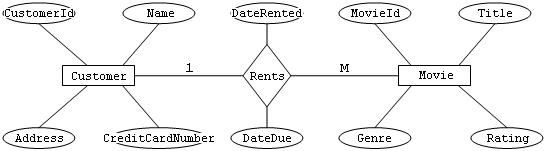
\includegraphics[scale=0.5]{er.png}
\caption{ER图}
\label{database_design}
\end{figure}

ER图用特定的形状来区分数据库的不同部分。矩形表示记录的类型(可以把它看作数据库对象的类)。椭圆表示记录的域(或属性)。菱形表示关系。

虽然ER图中各个元素的位置并不重要,但是认真布置它们,会更易于阅读,而且像Rents这样的关系也可以有自己的属性。

此外还要注意关系连接线上的标签,一边是1,一边是M。这些标号说明了关系的基数约束。基数约束限制了一次可以存在的关系数量。也就是说,基数约束代表的是在ER图中一次可以存在于两个实体间的关系数量。一般的基数关系有三种:

\begin{compactitem}
\item 一对一
\item 一对多
\item 多对多
\end{compactitem}

客户和电影之间的关系是一对多的,也就是说,一位客户可以租借多部电影,但(任何时刻)一部电影却只能被租借给一位客户。基数约束有助于数据库设计者表达关系的细节。


\section{数据库规范化}




\chapter{人工智能}


计算的一个子学科——人工智能(artificial intelligence,AI)向我们展示了计算的未来,计算机发展地更像人类了。另一方面,AI则是应用新技术来解决问题的途径。

AI处理的是人类思想的建模和应用,从普通的到怪异的,AI对许多类型的应用程序的开发都有影响,AI打开了新世界的大门,而这是计算领域的其他子学科做不到的。

AI在采用新技术的应用程序开发中扮演着至关重要的角色。

\section{图灵测试}

1950年,英国数学家Alan Turing发表了一篇具有里程碑性质的论文,其中提出了一个问题:机器能够思考吗?

在慎重地定义了术语智能和思维之后,最终他得出的结论是我们能够创造出可以思考的计算机,但他又提出了另一个问题:如何才能知道何时是成功了呢?

Turing对这个问题的答案叫做图灵测试(turing test),是确定一台机器是否能像人一样思考的衡量方法,图灵测试采用的方式是模拟人类对话。

图灵测试是一种行为方法,根据经验来判断一台计算机是否达到了智能化。这种测试的基础是一台计算机是否能够使人们相信它是另一个人。近年来出现了很多图灵测试的变体。

图灵测试是这样建立的,由一位质问者坐在一个房间中,用计算机终端与另外两个回答者A和B通信。质问者知道一位回答者是人,另一位回答者是计算机,但是不知道究竟哪个是人,哪个是计算机。如下图所示:

\begin{figure}[!ht]
\centering
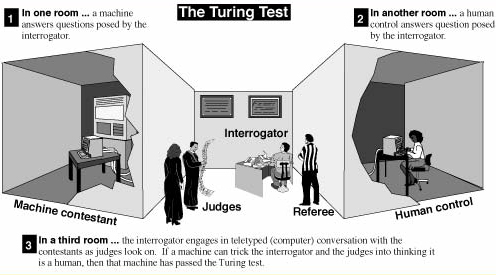
\includegraphics[scale=0.5]{turing_test.png}
\caption{图灵测试}
\label{turing_test}
\end{figure}

质问者分别与回答者A和B交谈之后,质问者要判断出哪个回答者是计算机。这个过程将由多个人反复执行。这个测试的假设是如果计算机能够瞒过足够多人,那么就可以把它看作是智能的。

第一次质问的情形当如此:

\begin{figure}[!h]
\centering
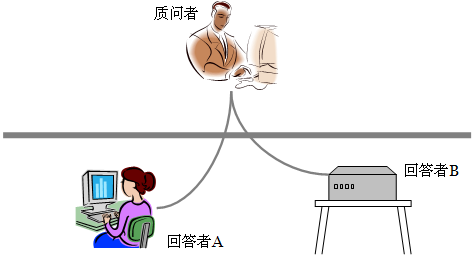
\includegraphics[scale=0.5]{turing_test_example.png}
\caption{第一次质问}
\label{turing_test_example}
\end{figure}

有些人认为图灵测试很适合测试计算机的智能,因为它要求计算机处理各种各样的知识,还要具有处理交谈中的变化所必需的灵活性。要瞒过质问人,计算机需要掌握的不仅仅是事实知识,还要注意人的行为和情绪。

另一些人则认为图灵测试并不能说明计算机理解了交谈的语言,而这一点对真正的智能来说是必需的。他们提出,程序能够模拟语言的内涵,可能足够使计算机通过图灵测试,但只凭这一点并不能说计算机智能化了。

通过图灵测试的计算机具有弱等价性(weak equivalence),即两个系统(人和计算机)在结果(输出)上是等价的,但实现这种结果的方式不同。强等价性(strong equivalence)说明两个系统使用的是相同的内部过程来生成结果。有些AI研究人员断言,只有实现了强等价性(即创造出了能像人一样处理信息的机器)才可能存在真正的人工智能。

这里,弱等价性指两个系统基于结果的等价性,强等价性指的是两个系统基于结果和实现这种结果的处理方法的等价性。

纽约慈善家Hugh Loebner组织了首次正式的图灵测试,Loebner prize成为了图灵测试的正式比赛。

虽然计算机的发展可以使得它们可以绘制复杂的三维图像,处理整个公司的工资表,判断正在建造的大桥是否能承受预计的交通压力。然而要它们理解人类的一个简单的对话却很困难。

人类对关于事物识别等类型的问题具有大量的知识和推理能力,而我们仍然在努力尝试用计算机执行类似人类的推理。

综上所述,在现代技术中,虽然计算机擅长技术,但却不擅长需要智能的任务,AI就是研究对人类思想建模颚应用人类智能的计算机系统的学科。

\section{AI问题的各个方面}



AI学科有很多需要研究的问题,导致现在AI有很多分支,最基本的问题是如何用计算机有效的处理形式表示知识。

目前AI涉及到的主要问题和还未解决的难题大致如下:

\begin{compactitem}
\item 知识表达——用于表示知识,以便计算机能够用来解决智能问题的技术。
\item 专家系统——嵌入人类专家知识的计算机系统。
\item 神经网络——模拟人脑处理的计算机系统。
\item 自然语言处理——处理人类用来交流的语言的难题。
\item 机器人学——关于机器人的研究
\end{compactitem}


\section{知识表达}


表示一个对象或事件所需的知识会根据情况而有所不同。对于要解决的问题,我们需要特定的信息。例如,如果要分析家族关系,那么就要知道Fred是Cathy的父亲,至于Fred是水管工,Cathy有台挖掘机这些信息就无关紧要了。而且我们需要的不仅仅是特定的信息,还需要一种形式,使我们能够有效地检索和处理信息。

表示知识的方法有很多种,可以用自然语言描述知识。例如,可以用一段英文描述一个学生以及他与外界的联系。尽管自然语言的说明性很强,但它不容易处理。所以我们需要形式化的语言,这里用一个近似于数学符号的符号表示学生,这种形式化更适合严格的计算机处理,但却难于理解和正确使用。

从某种程度上讲,AI中也存在数据结构的问题。我们想独立于数据的底层实现,创建它的逻辑视图,以便能用特殊的方式处理数据。不过,在AI领域,我们想捕捉的信息常常会产生有趣的新数据表示法。我们想捕捉的不止是事实,还有它们之间的关系。AI中知识表达要解决的问题的类型决定了要加于数据的结构。

在研究过特定的问题领域后,新的知识表达方法就会出现,比如语义网络和检索树等。




\subsection{语义网络}


语义网络(semantic network)是一种知识表达法,语义网络使用图形化方式表示知识,它捕捉了对象在真实世界中的关系。

语义网络的重点在于表示对象之间的关系。在表示语义网络的有向图中,节点表示对象,节点之间的箭头表示关系。箭号上的标签说明了关系的类型。根据网络图的分析可以回答问题。

语义网络借用了许多面向对象的概念,包括继承和实例化。继承关系说明一个对象是(is-a)另一个对象更具体的版本。实例化(instance-of)是一个真正的对象和这种对象的说明(如对象类)之间的关系。下图展示了一个语义网络,其中既有is-a关系,也有instance-of关系。此外还有其他类型的关系。在语义网络中,关系的类型基本上没有什么限制。


\begin{figure}[!ht]
\centering
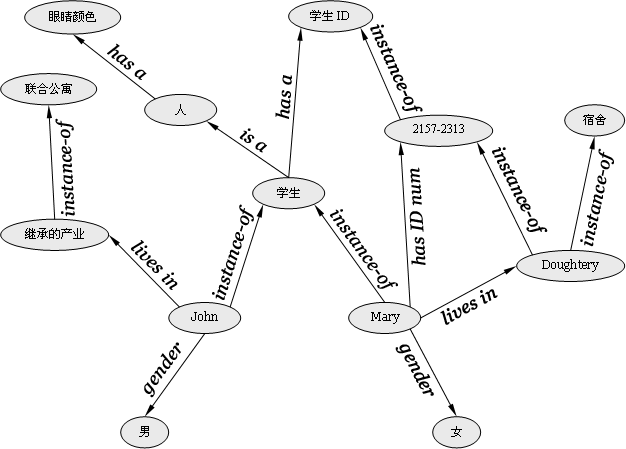
\includegraphics[scale=0.5]{semantic_network.png}
\caption{语义网络}
\label{semantic_network}
\end{figure}

在这个语义网络中还可以表示更多的关系,比如,可以说明每个人是惯用左手还是管用右手,或者说明John的汽车品牌,又或者说明每个学生的成绩。我们要表示的关系完全出于个人的选择,取决于回答我们面对的各种类型的问题所需要的信息。

建立关系的方法也有多种。例如,可以不说明每个学生所住的公寓,而说明每个公寓住了哪些学生。换句话说,可以反转箭头,把lives-in关系改成houses关系。同样地,这种选择也是在设计语义网络时由我们自己决定的。至于哪种方式更适合解决我们的问题,在某些情况下,我们会两者都选用。

语义网络所表示的关系的类型决定了哪些问题是可以轻松解决的,哪些是更难解决的,哪些是不能解决的。例如,用上述所示的语义网络,回答下列问题相当简单:

\begin{compactitem}
\item Mary是学生吗?
\item Mary的性别是什么?
\item Mary住在宿舍还是住在公寓?
\item Mary的学生ID是多少?
\end{compactitem}

但是,回答下面的问题却很困难。

\begin{compactitem}
\item 有多少女生,多少男生?
\item 谁住在Doughery?
\end{compactitem}

上述的语义网络是为表示学生个体与整个世界之间的关系而设计的,其中具有回答这些问题所必需的信息,差别仅仅在信息明显与否。但是如果需要找到所有学生,这里不存在这种信息。

这个语义网络不能回答下列问题,因为它没有表示必需的知识:


\begin{compactitem}
\item John开的是什么牌子的车子?
\item Mary的眼睛是什么颜色的?
\end{compactitem}



虽然已知Mary的眼睛具有一种颜色,因为她是学生,所有学生都是人,而所有人的眼睛都具有特定的颜色,只是根据网络中存储的信息,我们不知道Mary的眼睛究竟是什么颜色的。

语义网络是表示大量信息的强有力而通用的方式,难点在于建立正确的关系模型,用精确完整的数据填充整个网络。


\subsection{检索树}


在数据检索中,二叉树是只有两个、一个或没有子女的树,而一般的树结构的节点可能有多个子女。树在AI中扮演着重要的角色,在对抗性情况(如博弈)中,树用于表示各种可能的选择。

检索树是表示对抗性情况(如博弈)中的所有选择(知识)的结构,例如利用检索树(search tree)可以表示游戏中所有可能的移动(包括你和你的对手移动),可以创建一个游戏程序,最大化它获胜的机会。在某些情况下,甚至可以保证它总是获胜。

在二叉检索树中,只用一个值就可以确定是向右检索还是向左检索。在AI中使用的一般检索树中,一条路径表示玩家的一系列决定。每一层的决定说明了留给下一个玩家的选项。树中的每个节点表示一步移动,这个移动是以游戏中迄今为止已经发生的所有移动为基础的。

下面定义一个简单的Nim游戏作为示例,在这个例子中,一行有一定数量的空格。第一位玩家可以在最左边的一组空格中放入一个、两个或三个X。然后第二个玩家可以紧接着X放入一个、两个或三个O。游戏就这样由两个玩家轮流继续下去。谁把自己的符号放入了最后一个(最右边的)空格,谁就获胜。

下面是Nim游戏的玩法示例,其中使用了9个空格:






\section{专家系统}




\section{神经网络}




\section{自然语言处理}




\section{机器人学}





\chapter{模拟}




\chapter{图形和计算机辅助设计}





\chapter{Embedded System}

嵌入式系统是大型系统中专用于执行有限功能的计算机,嵌入式系统通常嵌在单个微处理器芯片上,程序存储在ROM中。几乎所有具有数字界面的用具都使用了嵌入式系统,如手表、微波炉、VCR和汽车等。

事实上,嵌入式系统无处不在,从电子产品到厨房用具,到汽车,到连网设备,到工业控制系统,处处都有嵌入式系统的应用。

有些嵌入式系统具有操作系统,但是大部分操作系统都是专用的,只需一个程序就可以实现全部的逻辑。

早期的嵌入式系统是独立的8位微处理器,自带操作系统。现在已经发展到32位的数字信号处理器(DSP),到64位的RISC(reduced instruction set,精简指令集)芯片等。而且,越来越多的嵌入式系统开始采用分布式微处理器网络,这种网络可以通过有线或无线的方式通信,由常规的网络管理通信协议远程监管和控制。

而且,事实上,术语嵌入式系统表达的不够清楚,因为它几乎包括除台式PC之外的所有机器。现在这个术语指的是预编译程序来执行大型系统中专门的或有限功能的计算机。其中暗示了终端用户或管理员(如果存在的话)会极少干涉这种系统。

由于一般人只是在厨房、客厅或汽车中遇到嵌入式系统,所以我们才会视嵌入式系统等同于硬件。但是,为嵌入式系统编写程序是必不可少的,而且要把程序烧录到系统附带的ROM(只读内存)中,以便它能够实现自己的作用。

由于不能在嵌入式处理器上开发和测试程序,因此,程序都是先在PC上编写,然后为目标系统进行编译,生成嵌入式系统的处理器能够执行的代码。

在早期的嵌入式系统中,代码的长度和执行速度都非常重要。由于汇编语言能够最有效地简化代码,加速程序的执行,所以汇编语言一直是嵌入式系统的专用语言。即使到C语言出现,并有了跨平台的C编译器后,汇编语言仍然继续被使用。C程序比汇编语言程序大约长和慢25\%,但是比较容易编写。

直到现在,ROM的大小仍然要求代码越短越好,所以汇编语言程序仍在使用。



\chapter{射频识别}


假想一下,我们在商店购买了一块电池,离开商店时,这块电池会“告诉”商店的售卖系统该补货了,因为电池的库存量很少了。射频识别技术(Radio-frequence identification,RFID)就使得这种情况成为可能。

如果给电池包装上安装一个RFID标签,它就能告诉中央射频器自己在哪里。除了应用于零售系统,RFID还用于跟踪货运集装箱、图书馆的藏书、汽车和动物等,人体中也可以植入RFID标签。

\part{Communication}

计算机在计算领域和通信领域都扮演着重要的角色,计算机之间的通信是通过计算机网络(Computer Network)实现的。计算机网络是为了通信和共享资源而以各种方式连在一起的一组计算设备,现在计算机网络也是一种基础设施,类似于复杂的高速公路系统,用各种方式把公路连接在一起,从而使汽车能够从出发点开到目的地。

计算机网络注重的是底层协议和数据传输率,通过计算机网络使数据能够从源计算机传送到目的计算机,接收数据的计算机的位置并不一定固定,但是当前地址是确定的。


\chapter{Network}

使用网络可以共享那些无形的资源(如文件)和有形的资源(如打印机)。Email、即时通信和网页都依赖于底层计算机网络中发生的通信。

计算机之间的连接通常是靠物理电线或电缆实现的,有些连接也可以使用无线电波或红外信号传导数据,这种连接是无线的,称为无线网络(Wireless Network)。

网络不是由物理连接定义的,而是由通信能力定义的。计算机网络中的设备不只是计算机,例如,打印机也可以直接连入网络,以便网络中的每个用户都可以使用它。此外,网络还包括各种处理网络信息传输的设备。我们用通用的术语节点(node)或主机(host)来引用网络中任何可寻址的设备。

计算机网络的一个关键问题是数据传输率(Data Transfer Rate),即数据从网络中的一个地点传输到另一个地点的速率。现在我们依靠网络传输更多更复杂(更大)的数据,比如多媒体等。

数据传输率又叫网络的带宽(Bandwidth)。在数据共享和传输过程中,网络固有的带宽限制定义了在固定时间内从一个地点传输到另一个地点的最大位数或字节数。

计算机网络的另一个关键问题是使用的协议(Protocol),协议说明了两个事物如何交互的一组规则,在计算术语中借用它来表示计算机在进行交互的时候使用的正确规定,或者说计算机网络通信协议是对那些计算机必须遵守以便彼此通信的的规则的描述。

计算机通信层的协议是一套规定必须严格遵守的规则和(交互信息的)过程的代码,在连网过程中,我们使用明确的协议来说明如何格式化和处理要传输的数据。

计算机网络开创了一个新的计算领域——客户/服务器模型(Client/Server Model)。计算机软件系统分布在整个网络中,在这个网络中,客户将向服务器请求信息或操作,服务器则对此做出响应。

例如,文件服务器(File Server)是网络中为多个用户存储和管理文件的计算机,这样每个用户不必都保存自己的文件副本。Web服务器(Web Server)是专用于响应(来自客户浏览器的)页面请求的计算机。现在,客户/服务器关系已经发展的非常复杂,而且客户/服务器模型在计算世界里也越来越重要了。

此外,现在客户/服务器模型除了支持基本的请求/响应功能之外,开始支持并行处理,即可以把一个问题分解为若干个小问题,然后用多台计算机来解决问题。使用计算机网络和客户/服务器模型,可以通过让客户请求多台机器执行一个问题的特定部分来实现并行处理,客户接收到每台机器的响应后,再把它们组合成一个完整的解决方案。

\section{Network Type}

计算机网络的分类方式有多种,通常根据网络的作用域对它们分类。局域网(Local Area Network,LAN)是连接较小地理范围的少量计算机的网络。LAN通常覆盖的是一个小的地理区域以及相对较少的互连设备,比如在一个房间或一幢建筑内,也可以延伸到几幢相邻的建筑中。管理LAN的各种配置叫做拓扑(Topology)。

环形拓扑(Ring Topology)把所有节点连接成一个封闭的环,消息在环中沿着一个方向传播。环形网络中的节点将传递消息,知道它们到达了目的地。星形拓扑(Star Topology)以一个节点为中心,其他节点都连接在中心节点上,所有消息都经过中心节点发送。星形网络给中心节点赋予了巨大的负荷,如果中心节点停止响应,那么整个网络的通信就瘫痪了。在总线拓扑(Bus Topology)中,所有节点都连接在一根通信线上,消息可以在通信线中双向传播。总线上的所有节点将检查总线传输的每个消息,不过如果消息所寻的地址不是该节点,它会忽略这条消息。以太网(Ethernet)的总线技术已经成为了局域网的业界标准。

\begin{figure}[!h]
\centering
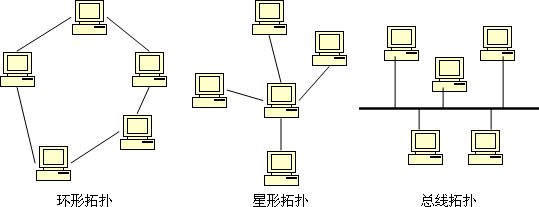
\includegraphics[scale=0.6]{network_topology.eps}
\caption{计算机网络拓扑}
\label{network_topology}
\end{figure}


广域网(Wide Area Network,WAN)是连接两个或多个相距较远的局域网的网络。网络之间的通信叫做网际互联,广域网使得较小的网络之间可以互相通信。

局域网中通常会有一个特殊节点作为网关(Gateway),处理当前局域网与其他网络之间的通信的就是网关。

\begin{figure}[!h]
\centering
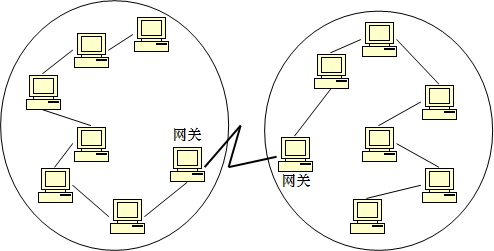
\includegraphics[scale=0.5]{network_gateway.png}
\caption{网关}
\label{network_gateway}
\end{figure}


城域网(Metropolitan Area Network,MAN),指的是在大城市内及其周边开发的基础通信设施,城域网络通常是采用创新技术(如光纤光缆)实现。


Internet本质上就是一个巨大的广域网,遍布整个地球,是所有的小网络的集合,这些小网络都采用相同的协议通信,而且会传递经过的消息,使它们能够到达最终目的地。

虽然术语Internet和Web常被混为一谈,但它们并不相同。万维网是分散在世界各处计算机上的信息和访问信息的软件构成的基础设施。而Web依靠底层网络(尤其是Internet)在用户之间交换信息。Web页不仅包含信息,还包含对其他资源(如图像等)的引用。由个人或公司管理的一组Web页叫做Web站点。全球各种Web页之间都有链接,这也是万维网这个名字的来源。




\section{Internet连接}


事实上,Internet(因特网)的概念,是1974年由温顿·瑟夫提出的。Internet作为一个广域网,它由多个小网络构成,这些小网络则通常属于某个人或某个公司,这些网络之间是如何连接的才真正定义了Internet,因此没有一个人或公司拥有Internet,甚至不能完整地控制它。


Internet骨干网(Internet Backbone)指的是承载Internet通信的一组高速网络。这些网络是由AT\&T、GTE和IBM这样的公司提供的。骨干网使用的是都是具有高数据传输率(从每秒1.5M到用特殊光缆实现的每秒600多兆位)的连接。

Internet服务提供者(Internet Service Provider,ISP)是给其他公司或个人提供Internet访问的公司,例如American Online等。ISP直接连接到Internet骨干网或者连接到更大的ISP。

把PC连接到Internet的方法有很多,最常用的三种方法是使用电话调制解调器、数字用户线路(DSL)或线缆调制解调器。

电话系统先于计算机网络进入千家万户,因此,以电话调制解调器作为家庭网络通信的首选方式就在情理之中。术语调制解调器(Modem)是调节器和解调器的缩写。


电话调制解调器将把计算机信息转换成模拟音频信号,以便在电话线中传输,目的地的调制解调器将把模拟音频信号转换回计算机信号。一种音频用于表示二进制的0,另一种用于表示1。

要使用电话调制解调器,必须首先将电脑与永久连接到Internet的计算机之间建立电话连接,而ISP就是通过这个连接来提供网络服务的。在给ISP付费后,就可以连接ISP提供的专用的计算机,建立连接后,就可以通过电话线把数据发送给ISP,ISP再把这些数据发送到Internet骨干网,传回的数据将被路由到你的ISP,最后发送到电脑上。

使用电话调制解调器不需要电话公司做任何特殊工作,而且数据被当作语音信号处理,所以除了在调制和解调的两端之外,不需要特殊的转换操作。


使用电话调制解调器连接的数据传输率被限制为模拟语音通信的数据传输率,最多每秒64Kbps。而如果把数据当作数字信号而不是模拟信号,那么电话线可以提供相当高的传输率,数字用户线路(Digital Subscriber Line,DSL)就是使用常规的铜质电话线传输数字信号的Internet连接方式。由于DSL和语音通信使用的频率不同,所以同一根电话线就可以满足这两种用途。


要建立DSL连接,首先电话公司要提供ISP服务,通过专门的计算机来处理数据通信。使用DSL,不必像电话调制解调器那样用拨电话的方式建立网络连接,DSL线路在PC与ISP之间维护了一个活动连接。不过由于数字信号在两点间传输的过程中会减弱,所以DSL传输速率会受到与ISP的专用计算机的距离的影响。


线缆调制解调器(Cable Modem)也是以数字形式来传输数据,不过采用的是有线电视信号的线缆,有线电视公司与ISP公司共享网络资源,提供线缆调制解调器的服务。

DSL连接和线缆调制解调器都属于宽带(Broadband)连接,即数据传输率至少为128Kbps,这两种方法提供的数据传输率都在每秒1.5M到3M之间。

DSL和线缆调制解调器的下载(Download)速度可以和上载(Upload)速度不同。


在 Internet 的早期,T1 连接被认为是非常快的连接。而今天的连接速度则要快得多。

在计算机网络中,1 字节等于 8 比特(这是用于传输一个字符的比特数),低速调制解调器能够传输大概 14 000 到 56 000 比特每秒(14 至 56 千比特每秒),即每秒传输 2000 至 7000 个字符,或大约 1 到 5 页文本。

一个千比特 (Kb) 是 1024 比特。一个兆比特 (Mb) 是 1024 千比特。一个 gigabit (Gb) 是 1024 兆比特。

下面是目前在 Internet 上被使用到的连接速度:

\begin{longtable}{|p{120pt}|p{120pt}|p{120pt}|}
%head
\multicolumn{3}{r}{}
\tabularnewline\hline
名称	&连接	&每秒的速度
\endhead
%endhead

%firsthead
\caption{Internet连接速度}\\
\hline
名称	&连接	&每秒的速度
\endfirsthead
%endhead

%foot
\multicolumn{3}{r}{}
\endfoot
%endfoot

%lastfoot
\endlastfoot
%endlastfoot
\hline
Modem		&Analog		&14.4-56Kb\\
\hline
D0			&Digital(ISDN)	&64Kb\\
\hline
T1			&Digital			&1.55Mb\\
\hline
T3			&Digital			&43Mb\\
\hline
OC-1		&Optical Carrier	&52Mb\\
\hline
OC-2		&Optical Carrier	&156Mb\\
\hline
OC-12		&Optical Carrier	&622Mb\\
\hline
OC-24		&Optical Carrier	&1.244Gb\\
\hline
OC-48		&Optical Carrier	&2.488Gb\\
\hline
\end{longtable}



\section{包交换}


ARPANET(阿帕网)作为全球互联网的鼻祖,第一次使用了报文交换技术,并且目前业已证实,该技术是由美国国防部高级研究计划局(DARPA)提供资金支持的。其设计初衷是,基于该技术建立的网络可用于各所大学与科研单位之间的相互交流,而不必担心网络连接不稳定问题。



但即便有国家国防部的资金投入,并不代表该项目必然与国防有所关联。同时,据项目负责人介绍,该项目更不会是出于躲避核袭击方面的考虑。鲍勃作为五角大楼的成员,当时也参与了该项目的运行,他表示ARPANET的设计动机决然和战争无关。



显然,没有阿帕网的建立,此后就没有互联网,更不要说预期利用网络覆盖达到抵御核攻击的宏伟目标了。事实上,对于阿帕网内部而言,关于分时性超级计算机的研发战略远比建立全球化军事网络为蓝图的战略部署要明确得多。




美国和英国的两个互联网研发小组,在大致相同的时间想到了报文交换技术。很多人认为,伦纳德和保尔在1969年发明了用以ARPANET的报文交换技术,但早在1965年,工作于英国国家物理研究室的研究员唐纳德便提交了分组交换的概念文档。


1967年,高级项目中介的项目管理经理约见了唐纳德,这两个不谋而合的研发小组自此开始强强联手,将成熟的报文交换技术最终用以ARPANET的建立。更有趣的是,报文交换技术是唐纳德最初的命名。

在20世纪70年代末,ARPANET上75\%以上的数据交换都来自于电子邮件(E-mail)。历史上第一封Email收信者和这封邮件的发出者都是同一个人,BBN公司(BroadBand Network)的网络工程师汤姆林森,他同时也是@这个邮箱符号的启用者。

为了提高在共享线路上传输信息的有效性,Internet上传输的消息被分割为大小固定、有编号的包(packet)。每个包将独立在网络上传输,直到到达目的地,它们将在此被重新组合为原始的消息,这种通信技术叫做包交换(Packet Switching)。

每个消息的包可以采用不同的路由线路,因此,它们到达目的地的顺序可能与发送顺序不同。需要把包按照正确顺序排列之后再组合成原始信息。


\begin{figure}[!h]
\centering
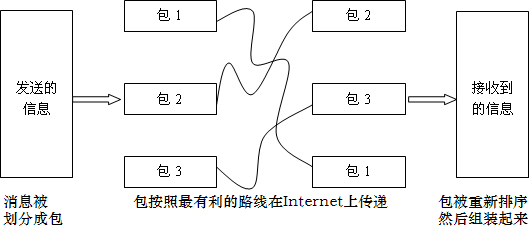
\includegraphics[scale=0.5]{network_pocket_switching.png}
\caption{包交换(Packet Switching)}
\label{network_pocket_switching}
\end{figure}

包在到达最终目的地之前,会在各种网络的计算机之间进行多次中转。用于指导包在网络之间传输的网络设备叫做路由器(Router)。中间的路由器不能规划包的整个传输路线,每个路由器只知道到达它的下一个目的地的最佳步骤。最终,消息将到达一个知道目的地机器的路由器。如果由于下行机器的问题中断了路径,或者选中的路径当前具有很大的通信量,那么路由器可能会把包发送给另一个路由器。

使用数字信号传输数据时,会有损失,使用中继器(Repeater)可以阻止这种情况发生。如果通信线路跨越的距离很长(如跨海的),那么线路上将安装中继器,以周期性地加强和传播信号。


\section{GPS}


GPS是全球定位系统(Global Positioning System)的缩写,即使用卫星技术查找25英尺之内的地点,这是一种用于确定方向的导航系统。


\chapter{Network Protocols}

计算机网络发展早期,不同的专有系统(Proprietary System)因为自己特有的差异导致不同类型的网络之间不能进行通信。

网络通信依靠协议支撑,由于这些原因(通常是历史原因),网络通信协议的大量出现,而且某些协议的地位比其他协议高。为了满足不同的网络之间互通信的需求,我们需要一种使不同的计算机系统能够通信的方式。


开放式系统(Open System)最大化了这种互通性(interoperability)的可能。


开放式系统的基础是一般的网络体系结构的通用模型和协议,它的实现采用了一系列协议,具有互通性。国际标准化组织ISO建立了开放式系统互连(OSI)参考模型来简化网络技术的开发。OSI参考模型在开放式系统的原则上把网络处理分成了7层,定义了一系列网络交互层,下面展示了OSI参考模型。

\begin{table}[!h]
\centering
\caption{OSI参考模型}
\label{Open_Systems_Interconnection_reference_model}
\begin{tabular}{|p{15pt}|p{80pt}|}
\hline
7	&应用层\\
\hline
6	&表示层\\
\hline
5	&会话层\\
\hline
4	&传输层\\
\hline
3	&网络层\\
\hline
2	&数据链路层\\
\hline
1	&物理层\\
\hline


\end{tabular}
\end{table}

开放式系统是以网络体系结构的通用模型为基础并且伴有一组协议的系统。开放式系统互连参考模型(Open Systems Interconnection reference model)是为了便于建立通信标准而对网络交互进行的7层逻辑划分。每一层处理网络通信的一个特定方面,最高层处理的是明确地与应用相关的问题。最低层处理的是与物理传输介质(如线型)相关的基础的电子或机械问题。其他层填补了其他各个方面,例如,网络层处理的是包的路由和寻址问题。之所以存在现在熟知的连网技术,都归功于开放式系统的技术和方法(如OSI参考模型)。






网络协议参照OSI参考模型的基本概念也进行了分层,以便OSI参考模型中的每一层都能依靠自己的基础协议,这样高层协议将以底层协议为支持。这种彼此依托的协议分层有时称为协议栈(Protocol Stack)。关键网络协议的分层示例如下:


\begin{figure}[!h]
\centering
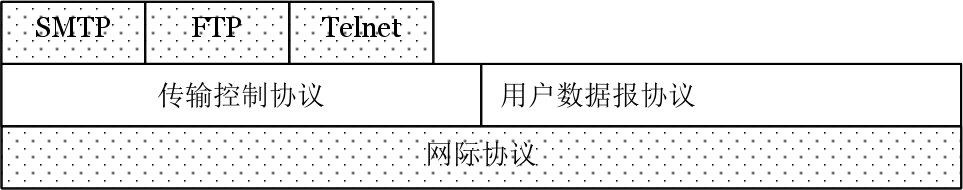
\includegraphics[scale=0.4]{network_protocol_stack.png}
\caption{协议栈(Protocol Stack)示例}
\label{network_protocol_stack}
\end{figure}


采用分层的方法,可以在不舍弃低层基础结构的前提下,开发新的协议。此外,这样还最小化了网络协议对网络处理其他方面的影响。有时,同一层中的协议提供同样的服务,但是采用的方式却不同。


上图中的最低两层构成了Internet通信的基础。其他协议有时叫做高层协议,负责处理特定类型的网络通信。这些层本质上是OSI参考模型的特定实现,以各种方式对应于该模型中的分层。


协议在某种意义上只是一种规约,规定了特定的数据类型必须按照特定的方式格式化,这些协议的重要之处在于它们提供了一种在连网的计算机之间进行交互的标准方式。文件格式的细节和数据域的大小对创建网络程序的开发者来说都是重要的。



\chapter{TCP/IP}


TCP/IP (Transmission Control Protocol / Internet Protocol)全称传输控制协议/网际协议\cite{tcp_ip},指的是一组协议和支持低层网络通信的工具程序,包含了一系列构成互联网基础的网络协议。

TCP/IP这种写法也反映了它们之间的关系,即TCP是在IP的基础之上的,同时也意味着TCP和IP在一起协同工作的,支持Internet通信的关键底层协议就是TCP/IP协议。



\section{History}


TCP/IP协议最早发源于美国国防部的ARPA网项目。TCP/IP模型也被称作DoD模型(Department of Defense Model)。TCP/IP字面上代表了两个协议:TCP(传输控制协议)和IP(网际协议)。

最初想到让不同电脑之间实现连接的,是美国加州大学洛杉矶分校网络工作小组的S.克罗克。1970年,克罗克及其小组着手制定最初的主机对主机通信协议,它被称为“网络控制协议”(NCP Network Control Protocol)。该协议被用于阿帕网,并在局部网络条件下运行稳定,但随着阿帕网用户的增多,NCP逐渐暴露出两大缺陷:

\begin{compactenum}
\item NCP只是一台主机对另一台主机的通讯协议,并未给网络中的每台电脑设置唯一的地址,结果就造成电脑在越来越庞大的网络中难以准确定位需要传输数据的对象。
\item NCP缺乏纠错功能,这样一来,数据在传输过程中一旦出现错误,网络就可能停止运行。出错电脑增多,使得网络运行效率大打折扣。
\end{compactenum}






最早的TCP/IP由文顿·瑟夫和罗伯特·卡恩两位开发,慢慢地通过竞争战胜了其他一些网络协议的方案,比如国际标准化组织ISO的OSI模型。TCP/IP的蓬勃发展发生在1990年代中期。当时一些重要而可靠的工具的出世,例如页面描述语言HTML和浏览器Mosaic,导致了互联网应用的飞速发展。

在构建了阿帕网先驱之后,DARPA开始了其他数据传输技术的研究。NCP诞生后两年,1972年,罗伯特·卡恩(Robert E. Kahn)被DARPA的信息技术处理办公室雇佣,在那里他研究卫星数据包网络和地面无线数据包网络,并且意识到能够在它们之间沟通的价值。在1973年春天,已有的ARPANET网络控制程序(NCP)协议的开发者文顿·瑟夫(Vinton Cerf)加入到卡恩为ARPANET设计下一代协议而开发开放互连模型的工作中。

到了1973年夏天,卡恩和瑟夫很快就开发出了一个基本的改进形式,其中网络协议之间的不同通过使用一个公用互联网络协议而隐藏起来,并且可靠性由主机保证而不是像ARPANET那样由网络保证。(瑟夫称赞Hubert Zimmerman和Louis Pouzin(CYCLADES网络的设计者)在这个设计上发挥了重要影响。)

由于网络的作用减少到最小的程度,就有可能将任何网络连接到一起,而不用管它们不同的特点,这样就解决了卡恩最初的问题。(一个流行的说法提到瑟夫和卡恩工作的最终产品TCP/IP将在运行“两个罐子和一根弦”上,实际上它已经用在信鸽上。一个称为网关(后来改为路由器以免与网关混淆)的计算机为每个网络提供一个接口并且在它们之间来回传输数据包。

这个设计思想更细的形式由瑟夫在斯坦福的网络研究组的1973年–1974年期间开发出来。(处于同一时期的诞生了PARC通用包协议组的施乐PARC早期网络研究工作也有重要的技术影响;人们在两者之间摇摆不定。)

DARPA于是与BBN、斯坦福和伦敦大学签署了协议开发不同硬件平台上协议的运行版本。有四个版本被开发出来——TCP v1、TCP v2、在1978年春天分成TCP v3和IP v3的版本,后来就是稳定的TCP/IP v4——目前因特网仍然使用的标准协议。

随着互联网的发展,目前流行的IPv4协议(网际协议版本四)已经接近它的功能上限。IPv4最致命的两个缺陷在于:

\begin{compactitem}
\item 地址只有32位,IP地址空间有限;
\item 不支持服务质量(Quality of Service,QoS)的想法,无法管理带宽和优先级,故而不能很好的支持现今越来越多的实时的语音和视频应用。因此IPv6(网际协议版本六)浮出水面,用以取代IPv4。
\end{compactitem}

1975年,两个网络之间的TCP/IP通信在斯坦福和伦敦大学(UCL)之间进行了测试。1977年11月,三个网络之间的TCP/IP测试在美国、英国和挪威之间进行。在1978年到1983年间,其他一些TCP/IP原型在多个研究中心之间开发出来。ARPANET完全转换到TCP/IP在1983年1月1日发生。

1983年1月1日,在因特网的前身(ARPA网)中,TCP/IP协议取代了旧的网络控制协议(NCP,Network Control Protocol),从而成为今天的互联网的基石。

1984年,美国国防部将TCP/IP作为所有计算机网络的标准。1985年,因特网架构理事会举行了一个三天有250家厂商代表参加的关于计算产业使用TCP/IP的工作会议,帮助协议的推广并且引领它日渐增长的商业应用。

2005年9月9日卡恩和瑟夫由于他们对于美国文化做出的卓越贡献被授予总统自由勋章。


TCP/IP成功的另一个因素在于对为数众多的低层协议的支持。这些低层协议对应OSI模型中的第一层(实体层)和第二层(数据链路层)。每层的所有协议几乎都有一半数量支持TCP/IP,例如:以太网(Ethernet)、令牌环(Token Ring)、光纤数据分布接口(FDDI)、端对端协议(PPP)、X.25、帧中继(Frame Relay)、ATM、Sonet、SDH等。

\section{Key Architectural Principles}



TCP/IP 是供已连接因特网的计算机进行通信的通信协议,通信协议是对计算机必须遵守的规则的描述,只有遵守这些规则,计算机之间才能进行通信。

整个通信网络的任务,可以划分成不同的功能区块,即所谓的层级(layer)。用于互联网的协议可以比照TCP/IP参考模型进行分类。TCP/IP协议栈起始于第三层协议IP(网际协议)。所有这些协议都在相应的RFC文档中讨论及标准化。重要的协议在相应的RFC文档中均标记了状态:“必须”(required),“推荐”(recommended),“可选”(elective)。其他的协议还可能有“试验”(experimental)或“历史”(historic)的状态。”



浏览器和服务器均使用 TCP/IP 来连接Internet。浏览器使用 TCP/IP 来访问服务器,服务器使用 TCP/IP 向浏览器传回 HTML,电子邮件程序也是使用 TCP/IP与Internet连接的,这样才能收发邮件。

\begin{compactitem}
\item TCP协议和软件负责把消息分割成包,交给IP软件传递,目的地机器上的TCP则负责把包排序,重新组合成信息,并负责处理错误。TCP软件还要处理所有发生的错误,如一个包永远不能到达目的地。

简单的说,TCP控制应用程序之间的通信。

\item IP协议和软件处理的是包通过互相连接的网络传递到最终目的地的路由选择,或者说,IP协议和软件负责包的路由,将包发送至接受者。

简单的说,IP控制计算机之间的通信。


\item UDP是用户数据报协议(User Datagram Protocol)的缩写,它是TCP的替代品,控制应用程序之间的简单通信。

简单的说,UDP软件的角色基本上与TCP软件一样,主要的不同之处在于TCP牺牲了一定的性能,提供了高度可靠性,而UDP更快,但不那么可靠。
\end{compactitem}

\begin{figure}[!ht]
\centering
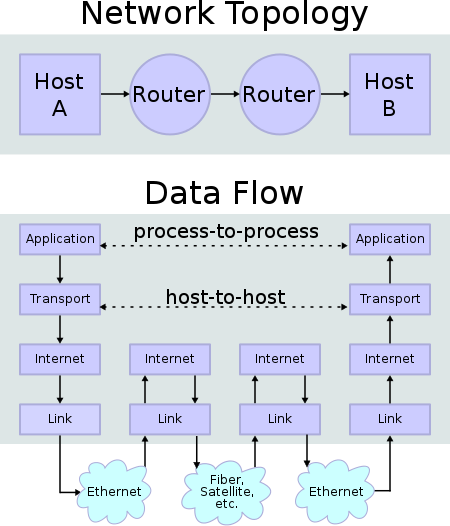
\includegraphics[scale=0.5]{IP_stack_connections.png}
\caption{两个因特网主机通过两个路由器和对应的层连接。各主机上的应用通过一些数据通道相互执行读取操作。}
\label{IP_stack_connections}
\end{figure}



UDP也是TCP/IP协议组的一部分,由于TCP是高度可靠的,还出于一定的历史原因,所以这套协议叫做TCP/IP协议。现在,TCP/IP被用来指称基于 TCP 和 IP 这两个最初的协议之上的不同的通信协议的大的集合(协议族),因特网地址\textcolor{Blue}{XXX.XXX.XXX.XXX}也是标准的 TCP/IP 协议的一部分。


所有的TCP/IP应用都必须实现IP和ICMP。对于一个路由器(router)而言,有这两个协议就可以运作了,虽然从应用的角度来看,这样一个路由器意义不大。实际的路由器一般还需要运行许多“推荐”使用的协议,以及一些其他的协议。

这样,TCP/IP 定义了电子设备(比如计算机)如何连入因特网,以及数据如何在它们之间传输的标准,其中:

\begin{compactitem}
\item TCP 使用固定的连接

当应用程序希望通过 TCP 与另一个应用程序通信时,它会发送一个通信请求。这个请求必须被送到一个确切的地址。在双方“握手”之后,TCP 将在两个应用程序之间建立一个全双工 (full-duplex) 的通信。

这个全双工的通信将占用两个计算机之间的通信线路,直到它被一方或双方关闭为止。UDP 和 TCP 很相似,但是更简单,同时可靠性低于 TCP。

\item IP 是无连接的

IP 是无连接的通信协议,它不会占用两个正在通信的计算机之间的通信线路。这样,IP 就降低了对网络线路的需求。每条线可以同时满足许多不同的计算机之间的通信需要。

通过 IP,消息(或者其他数据)被分割为小的独立的数据包,并通过因特网在计算机之间传送。在这个过程中,IP 负责将每个数据包路由至它的目的地。
\end{compactitem}

\zihao{6}

\begin{longtable}{|p{30pt}|p{110pt}|p{240pt}|}
%head
\multicolumn{3}{r}{}
\tabularnewline\hline
协议	& 名称 & 描述
\endhead
%endhead

%firsthead
\caption{网络通信协议集合}\\
\hline
协议	& 名称 & 描述
\endfirsthead
%endfirsthead

%foot
\multicolumn{3}{r}{}
\endfoot
%endfoot

%lastfoot
\endlastfoot
%endlastfoot
\hline
TCP		&传输控制协议						&TCP 用于从应用程序到网络的数据传输控制,负责在数据传送之前将它们分割为 IP 包,然后在它们到达的时候将它们重组。\\
\hline
IP		&网际协议							&IP 负责计算机之间的通信,负责在因特网上发送和接收数据包。\\
\hline
HTTP	&超文本传输协议						&HTTP 负责 web 服务器与 web 浏览器之间的通信,用于从 web 客户端(浏览器)向 web 服务器发送请求,并从 web 服务器向 web 客户端返回内容(网页)。\\
\hline
HTTPS	&安全的 HTTP						&HTTPS 负责在 web 服务器和 web 浏览器之间的安全通信。作为有代表性的应用,HTTPS 会用于处理信用卡交易和其他的敏感数据。\\
\hline
SSL		&安全套接字层						&SSL 协议用于为安全数据传输加密数据。\\
\hline
SMTP	&简易邮件传输协议					&SMTP 用于电子邮件的传输。\\
\hline
MIME	&多用途因特网邮件扩展				&MIME 协议使 SMTP 有能力通过 TCP/IP 网络传输多媒体文件,包括声音、视频和二进制数据。	\\
\hline
IMAP	&因特网消息访问协议					&IMAP 用于存储和取回电子邮件。\\
\hline
POP		&邮局协议							&POP 用于从电子邮件服务器向个人电脑下载电子邮件。\\
\hline
FTP		&文件传输协议						&FTP 负责计算机之间的文件传输。\\
\hline
NTP		&网络时间协议						&NTP 用于在计算机之间同步时间(钟)。\\
\hline
DHCP	&动态主机配置协议					&DHCP 用于向网络中的计算机分配动态 IP 地址。\\
\hline
SNMP	&简单网络管理协议					&SNMP 用于计算机网络的管理。\\
\hline
LDAP	&轻量级的目录访问协议				&LDAP 用于从因特网搜集关于用户和电子邮件地址的信息。\\
\hline
ICMP	&因特网消息控制协议					&ICMP 负责网络中的错误处理。\\
\hline
ARP		&Address Resolution Protocol			&ARP用于通过 IP 来查找基于 IP 地址的计算机网卡的硬件地址。\\
\hline
RARP	&Reverse Address Resolution Protocol	&RARP 用于通过 IP 查找基于硬件地址的计算机网卡的 IP 地址。\\
\hline
BOOTP	&Boot Protocol						&BOOTP 用于从网络启动计算机。\\
\hline
PPTP	&点对点隧道协议						&PPTP 用于私人网络之间的连接(隧道)。\\
\hline

\end{longtable}

\zihao{5}

其中:

\begin{compactitem}
\item 一个简单的路由器上可能会实现ARP,IP,ICMP,UDP,SNMP,RIP。
\item WWW用户端使用ARP,IP,ICMP,UDP,TCP,DNS,HTTP,FTP。
\item 一台用户电脑上还会运行如TELNET,SMTP,POP3,SNMP,ECHO,DHCP,SSH,NNTP。
\item 无盘设备可能会在固件,比如ROM中实现了ARP,IP,ICMP,UDP,BOOT,TFTP(均为面向数据包的协议,实现起来相对简单)。
\end{compactitem}


IP程序ping可以用于测试网络指派的可达性,即一台特定的网络计算机是否是活动的以及是否可到达,每个运行IP软件的计算机都会对ping请求做出回应,这使得ping成了一种方便的测试方式,无论特定的计算机是否在运行,也无论是否能通过网络达到它。

ping是Packet InterNet Groper的正式缩写,这个名称来源于潜水艇发送一个声纳脉冲,然后侦听返回的回声所采用的术语。由于ping是在IP层运行的,所以即使高层协议没有响应,它常常也会做出反应。

另一种TCP/IP工具叫做跟踪路由程序(traceroute),用于展示包在到达目的节点的过程中经过的路线,跟踪路由程序输出的是作为中转站的计算机的列表。


当一个 IP 包从一台计算机被发送,它会到达一个 IP 路由器。IP 路由器负责将这个包路由至它的目的地,直接地或者通过其他的路由器。

在一个相同的通信中,一个包所经由的路径可能会和其他的包不同。而路由器负责根据通信量、网络中的错误或者其他参数来进行正确地寻址。

几乎所有连接到互联网上的电脑上都存在的IPv4协议出生在1981年,今天的版本和最早的版本并没有多少改变。升级版IPv6的工作始于1995年,目的在于取代IPv4。ICMP协议主要用于收集有关网络的信息查找错误等工作。

\section{TCP/IP \& OSI}

TCP/IP参考模型是一个抽象的分层模型,这个模型中,所有的TCP/IP系列网络协议都被归类到4个抽象的"层"中。每一抽象层建立在低一层提供的服务上,并且为高一层提供服务。

完成一些特定的任务需要众多的协议协同工作,这些协议分布在参考模型的不同层中的,因此有时称它们为一个协议栈。

TCP/IP参考模型为TCP/IP协议栈订身制作。其中IP协议只关心如何使得数据能够跨越本地网络边界的问题,而不关心如何利用传输媒体,数据如何传输。整个TCP/IP协议栈则负责解决数据如何通过许许多多个点对点通路(一个点对点通路,也称为一``跳", 1 hop)顺利传输,由此不同的网络成员能够在许多``跳"的基础上建立相互的数据通路。

如想分析更普遍的网络通信问题,ISO的OSI模型也能起更好的帮助作用。

因特网协议族是一组实现支持因特网和大多数商业网络运行的协议栈的网络传输协议。它有时也被称为TCP/IP协议组,这个名称来源于其中两个最重要的协议:传输控制协议(TCP)和因特网协议(IP),它们也是最先定义的两个协议。

同许多其他协议一样网络传输协议也可以看作一个多层组合,每层解决数据传输中的一组问题并且向使用这些低层服务的高层提供定义好的服务。高层逻辑上与用户更为接近,所处理数据更为抽象,它们依赖于低层将数据转换成最终能够进行实体控制的形式。

网络传输协议能够大致匹配到一些厂商喜欢使用的固定7层的OSI模型。然而这些层并非都能够很好地与基于ip的网络对应(根据应用的设计和支持网络的不同它们确实是涉及到不同的层)并且一些人认为试图将因特网协议组对应到OSI会带来混淆而不是有所帮助。


\section{Internet Protocols Layers}

人们已经进行了一些讨论关于如何将TCP/IP参考模型映射到OSI模型。由于TCP/IP和OSI模型组不能精确地匹配,还没有一个完全正确的答案。

另外,OSI模型下层还不具备能够真正占据真正层的位置的能力;在传输层和网络层之间还需要另外一个层(网络互连层)。特定网络类型专用的一些协议应该运行在网络层上,但是却运行在基本的硬件帧交换上。类似协议的例子有地址解析协议和生成树协议(用来保持冗余网桥的空闲状态直到真正需要它们)。然而,它们是本地协议并且在网络互连功能下面运行。不可否认,将两个组(更不用说它们只是运行在如ICMP等不同的互连网络协议上的逻辑上的网络层的一部分)整个放在同一层会引起混淆,但是OSI模型还没有复杂到能够做更好的工作。


下面的图表试图显示不同的TCP/IP和其他的协议在最初OSI模型中的位置:



\begin{table}[!htbp]
\centering
\rowcolors{1}{White}{Lavender}
\begin{tabular}{l|l|l|}
\cline{2-3}
7&应用层&{\small HTTP,SMTP,SNMP,FTP,Telnet,SIP,SSH,NFS,RTSP,XMPP,Whois,ENRP等}\\ 
6&表示层&{\small XDR,ASN.1,SMB,AFP,NCP等}\\ 
5&会话层&{\small ASAP,SSH,ISO 8327/CCITT X.225,RPC,NetBIOS,ASP,Winsock,BSD sockets等}\\ 
4&传输层&{\small TCP,UDP,TLS,RTP,SCTP,SPX,ATP,IL等}\\ 
3&网络层&{\small IP,ICMP,IGMP,IPX,BGP,OSPF,RIP,IGRP,EIGRP,ARP,RARP,X.25等}\\ 
2&数据链路层&{\small 以太网,令牌环,HDLC,帧中继,ISDN,ATM,IEEE 802.11,FDDI,PPP等}\\ 
1&实体层&{\small 线路,无线电,光纤等}\\ \cline{2-3}
\end{tabular}
\end{table}


通常人们认为OSI模型的最上面三层(应用层、表示层和会话层)在TCP/IP组中是一个应用层。由于TCP/IP有一个相对较弱的会话层,由TCP和RTP下的打开和关闭连接组成,并且在TCP和UDP下的各种应用提供不同的端口号,这些功能能够被单个的应用程序(或者那些应用程序所使用的库)增加。与此相似的是,IP是按照将它下面的网络当作一个黑盒子的思想设计的,这样在讨论TCP/IP的时候就可以把它当作一个独立的层。

\begin{table}[!ht]
\centering
\rowcolors{1}{White}{Lavender}
\begin{tabular}{m{10pt}|m{60pt}|m{310pt}|}
\cline{2-3}
4&{\footnotesize 应用层\newline (OSI 5到7层)}&{\footnotesize 例如HTTP,FTP,DNS(如BGP和RIP这样的路由协议,尽管由于各种各样的原因它们分别运行在TCP和UDP上,仍然可以将它们看作网络层的一部分)}\\
3&{\footnotesize 传输层\newline (OSI 4层)}&{\footnotesize 例如TCP,UDP,RTP,SCTP(如OSPF这样的路由协议,尽管运行在IP上也可以看作是网络层的一部分)}\\
2&{\footnotesize 网络互连层\newline (OSI 3层)}&{\footnotesize 对于TCP/IP来说这是因特网协议(IP)(如ICMP和IGMP这样的必须协议尽管运行在IP上,也仍然可以看作是网络互连层的一部分;ARP不运行在IP上)}\\
1&{\footnotesize 网络接口层\newline (OSI 1和2层)}&{\footnotesize 例如以太网,Wi-Fi,MPLS等。}\\ \cline{2-3}
\end{tabular}
\end{table}


\subsection{应用层}


该层包括所有和应用程序协同工作,利用基础网络交换应用程序专用的数据的协议。 应用层是大多数普通与网络相关的程序为了通过网络与其他程序通信所使用的层。这个层的处理过程是应用特有的;数据从网络相关的程序以这种应用内部使用的格式进行传送,然后被编码成标准协议的格式。

一些特定的程序被认为运行在这个层上。它们提供服务直接支持用户应用。这些程序和它们对应的协议包括HTTP(万维网服务)、FTP(文件传输)、SMTP(电子邮件)、SSH(安全远程登陆)、DNS(名称<-> IP地址寻找)以及许多其他协议。
一旦从应用程序来的数据被编码成一个标准的应用层协议,它将被传送到IP栈的下一层。

在传输层,应用程序最常用的是TCP或者UDP,并且服务器应用程序经常与一个公开的端口号相联系。服务器应用程序的端口由互联网号码分配局(IANA)正式地分配,但是现今一些新协议的开发者经常选择它们自己的端口号。由于在同一个系统上很少超过少数几个的服务器应用,端口冲突引起的问题很少。应用软件通常也允许用户强制性地指定端口号作为运行参数。

连结外部的客户端程序通常使用系统分配的一个随机端口号。监听一个端口并且通过服务器将那个端口发送到应用的另外一个副本以建立对等连结(如IRC上的dcc文件传输)的应用也可以使用一个随机端口,但是应用程序通常允许定义一个特定的端口范围的规范以允许端口能够通过实现网络地址转换(NAT)的路由器映射到内部。

每一个应用层(TCP/IP参考模型的最高层)协议一般都会使用到两个传输层协议之一: 面向连接的TCP传输控制协议和无连接的包传输的UDP用户数据报文协议。

常用的应用层协议有:

\begin{compactitem}
\item 运行在TCP协议上的协议:

	\begin{compactitem}
	\item HTTP(Hypertext Transfer Protocol,超文本传输协议),主要用于普通浏览。
	\item HTTPS(Hypertext Transfer Protocol over Secure Socket Layer, or HTTP over SSL,安全超文本传输协议),HTTP协议的安全版本。
	\item FTP(File Transfer Protocol,文件传输协议),由名知义,用于文件传输。
	\item POP3(Post Office Protocol, version 3,邮局协议),收邮件用。
	\item SMTP(Simple Mail Transfer Protocol,简单邮件传输协议),用来发送电子邮件。
	\item TELNET(Teletype over the Network,网络电传),通过一个终端(terminal)登陆到网络。
	\item SSH(Secure Shell,用于替代安全性差的TELNET),用于加密安全登陆用。
	\end{compactitem}
\item 运行在UDP协议上的协议:
	\begin{compactitem}
	\item BOOTP(Boot Protocol,启动协议),应用于无盘设备。
	\item NTP(Network Time Protocol,网络时间协议),用于网络同步。
	\end{compactitem}
\item 其他:
	\begin{compactitem}
	\item DNS(Domain Name Service,域名服务),用于完成地址查找,邮件转发等工作(运行在TCP和UDP协议上)。
	\item ECHO(Echo Protocol,回绕协议),用于查错及测量应答时间(运行在TCP和UDP协议上)。
	\item SNMP(Simple Network Management Protocol,简单网络管理协议),用于网络信息的收集和网络管理。
	\item DHCP(Dynamic Host Configuration Protocol,动态主机配置协议),动态配置IP地址。
	\item ARP(Address Resolution Protocol,地址解析协议),用于动态解析以太网硬件的地址。
	\end{compactitem}
\end{compactitem}





\subsection{传输层}

传输层的协议,能够解决诸如端到端可靠性(“数据是否已经到达目的地?”)和保证数据按照正确的顺序到达这样的问题。在TCP/IP协议组中,传输协议也包括所给数据应该送给哪个应用程序。

在TCP/IP协议组中技术上位于这个层的动态路由协议通常被认为是网络层的一部分;一个例子就是OSPF(IP协议89)。

TCP(IP协议6)是一个“可靠的”、面向连结的传输机制,它提供一种可靠的字节流保证数据完整、无损并且按顺序到达。TCP尽量连续不断地测试网络的负载并且控制发送数据的速度以避免网络过载。另外,TCP试图将数据按照规定的顺序发送。这是它与UDP不同之处,这在实时数据流或者路由高网络层丢失率应用的时候可能成为一个缺陷。

较新的SCTP也是一个“可靠的”、面向连结的传输机制。它是面向纪录而不是面向字节的,它在一个单独的连结上提供了通过多路复用提供的多个子流。它也提供了多路自寻址支持,其中连结终端能够被多个IP地址表示(代表多个实体接口),这样的话即使其中一个连接失败了也不中断。它最初是为电话应用开发的(在IP上传输SS7),但是也可以用于其他的应用。

UDP(IP协议号17)是一个无连结的数据报协议。它是一个“尽力传递”(best effort)或者说“不可靠”协议——不是因为它特别不可靠,而是因为它不检查数据包是否已经到达目的地,并且不保证它们按顺序到达。如果一个应用程序需要这些特性,那它必须自行检测和判断,或者使用TCP协议。

UDP的典型性应用是如流媒体(音频和视频等)这样按时到达比可靠性更重要的应用,或者如DNS查找这样的简单查询/响应应用,如果建立可靠的连结所作的额外工作将是不成比例地大。

DCCP目前正由IEFT开发。它提供TCP流动控制语义,但对于用户来说保留了UDP的数据报服务模型。

TCP和UDP都用来支持一些高层的应用。任何给定网络地址的应用通过它们的TCP或者UDP端口号区分。根据惯例使一些大众所知的端口与特定的应用相联系。

RTP是为如音频和视频流这样的实时数据设计的数据报协议。RTP是使用UDP包格式作为基础的会话层,然而据说它位于因特网协议栈的传输层。




\subsection{网络互连层}

正如最初所定义的,网络层解决在一个单一网络上传输数据包的问题。类似的协议有X.25和ARPANET的Host/IMP Protocol。

随着因特网思想的出现,在这个层上添加了附加的功能,也就是将数据从源网络传输到目的网络。这就牵涉到在网络组成的网上选择路径将数据包传输,也就是因特网。

在因特网协议组中,IP完成数据从源发送到目的的基本任务。IP能够承载多种不同的高层协议的数据;这些协议使用一个唯一的IP协议号进行标识。ICMP和IGMP分别是1和2。

一些IP承载的协议,如ICMP(用来发送关于IP发送的诊断信息)和IGMP(用来管理多播数据),它们位于IP层之上但是完成网络层的功能,这表明了因特网和OSI模型之间的不兼容性。所有的路由协议,如BGP、OSPF、和RIP实际上也是网络层的一部分,尽管它们似乎应该属于更高的协议栈。






\subsection{网络接口层}



网络接口层实际上并不是因特网协议组中的一部分,但是它是数据包从一个设备的网络层传输到另外一个设备的网络层的方法。这个过程能够在网卡的软件驱动程序中控制,也可以在韧体或者专用芯片中控制。这将完成如添加报头准备发送、通过实体媒介实际发送这样一些数据链路功能。另一端,链路层将完成数据帧接收、去除报头并且将接收到的包传到网络层。

然而,链路层并不经常这样简单。它也可能是一个虚拟专有网络(VPN)或者隧道,在这里从网络层来的包使用隧道协议和其他(或者同样的)协议组发送而不是发送到实体的接口上。VPN和隧道通常预先建好,并且它们有一些直接发送到实体接口所没有的特殊特点(例如,它可以加密经过它的数据)。由于现在链路“层”是一个完整的网络,这种协议组的递归使用可能引起混淆。但是它是一个实现常见复杂功能的一个优秀方法。(尽管需要注意预防一个已经封装并且经隧道发送下去的数据包进行再次地封装和发送)。










在长期的发展过程中,IP逐渐取代其他网络。这里是一个简单的解释。IP传输通用数据。数据能够用于任何目的,并且能够很轻易地取代以前由专有数据网络传输的数据。下面是一个普通的过程:

\begin{compactenum}
\item 一个专有的网络开发出来用于特定目的。如果它工作很好,用户将接受它。
\item 为了便利提供IP服务,经常用于访问电子邮件或者聊天,通常以某种方式通过专有网络隧道实现。隧道方式最初可能非常没有效率,因为电子邮件和聊天只需要很低的带宽。
\item 通过一点点的投资IP基础设施逐渐在专有数据网络周边出现。
\item 用IP取代专有服务的需求出现,经常是一个用户要求。
\item IP替代品过程遍布整个因特网,这使IP替代品比最初的专有网络更加有价值(由于网络效应)。
\item 专有网络受到压制。许多用户开始维护使用IP替代品的复制品。
\item IP包的间接开销很小,少于1\%,这样在成本上非常有竞争性。人们开发了一种能够将IP带到专有网络上的大部分用户的不昂贵的传输媒介。
\item 大多数用户为了削减开销,专有网络被取消。
\end{compactenum}

如今,大多数商业操作系统包括TCP/IP栈并且缺省安装它们,对于大多数用户来说,没有必要去寻找它们的实现。TCP/IP包含在所有的商业Unix和Linux发布包中,同样也包含在Mac OS X和微软视窗和视窗服务器版本中。





















\chapter{HTTP}



\section{HTTP State Message}


当浏览器从Web服务器请求服务时,可能会发生错误,从而有可能会返回下面的一系列状态消息:


\begin{longtable}{|p{140pt}|p{260pt}|}

%head
\multicolumn{2}{r}{...}
\tabularnewline\hline
消息			&描述		
\endhead

%firsthead
\caption{1xx: 信息}\\
\hline
消息			&描述
\endfirsthead


%foot
\multicolumn{2}{r}{...}
\endfoot


\endlastfoot

\hline
100 Continue				&服务器仅接收到部分请求,但是一旦服务器并没有拒绝该请求,客户端应该继续发送其余的请求。\\
\hline
101 Switching Protocols	&服务器转换协议:服务器将遵从客户的请求转换到另外一种协议。							\\
\hline
\end{longtable}


\begin{longtable}{|p{140pt}|p{260pt}|}

%head
\multicolumn{2}{r}{...}
\tabularnewline\hline
消息			&描述		
\endhead

%firsthead
\caption{2xx: 成功}\\
\hline
消息			&描述
\endfirsthead


%foot
\multicolumn{2}{r}{...}
\endfoot


\endlastfoot

\hline
200 OK							&请求成功(其后是对GET和POST请求的应答文档。)\\
\hline
201 Created						&请求被创建完成,同时新的资源被创建。\\
\hline
202 Accepted						&供处理的请求已被接受,但是处理未完成。\\
\hline
203\newline Non-authoritative Information	&文档已经正常地返回,但一些应答头可能不正确,因为使用的是文档的拷贝。\\
\hline
204 No Content					&没有新文档。浏览器应该继续显示原来的文档。如果用户定期地刷新页面,而Servlet可以确定用户文档足够新,这个状态代码是很有用的。\\
\hline
205 Reset Content					&没有新文档。但浏览器应该重置它所显示的内容。用来强制浏览器清除表单输入内容。\\
\hline
206 Partial Content				&客户发送了一个带有Range头的GET请求,服务器完成了它。\\
\hline
\end{longtable}








\begin{longtable}{|p{140pt}|p{260pt}|}

%head
\multicolumn{2}{r}{...}
\tabularnewline\hline
消息			&描述		
\endhead

%firsthead
\caption{3xx: 重定向}\\
\hline
消息			&描述
\endfirsthead


%foot
\multicolumn{2}{r}{...}
\endfoot


\endlastfoot

\hline
300 Multiple Choices		&多重选择。链接列表。用户可以选择某链接到达目的地。最多允许五个地址。\\
\hline
301 Moved Permanently	&所请求的页面已经转移至新的url。\\
\hline
302 Found				&所请求的页面已经临时转移至新的url。\\
\hline
303 See Other			&所请求的页面可在别的url下被找到。\\
\hline
304 Not Modified			&未按预期修改文档。客户端有缓冲的文档并发出了一个条件性的请求(一般是提供If-Modified-Since头表示客户只想比指定日期更新的文档)。服务器告诉客户,原来缓冲的文档还可以继续使用。\\
\hline
305 Use Proxy			&客户请求的文档应该通过Location头所指明的代理服务器提取。\\
\hline
306 Unused				&此代码被用于前一版本。目前已不再使用,但是代码依然被保留。\\
\hline
307 Temporary Redirect		&被请求的页面已经临时移至新的url。\\
\hline
\end{longtable}





\begin{longtable}{|p{140pt}|p{260pt}|}

%head
\multicolumn{2}{r}{...}
\tabularnewline\hline
消息			&描述		
\endhead

%firsthead
\caption{4xx: 客户端错误}\\
\hline
消息			&描述
\endfirsthead


%foot
\multicolumn{2}{r}{...}
\endfoot


\endlastfoot
\hline
400 Bad Request		&服务器未能理解请求。\\
\hline
401 Unauthorized		&被请求的页面需要用户名和密码。\\
\hline
402 Payment Required	&此代码尚无法使用。\\
\hline
403 Forbidden		&对被请求页面的访问被禁止。\\
\hline
404 Not Found		&服务器无法找到被请求的页面。\\
\hline
405 Method Not Allowed&	请求中指定的方法不被允许。\\
\hline
406 Not Acceptable	&服务器生成的响应无法被客户端所接受。\\
\hline
407\newline Proxy Authentication Required&	用户必须首先使用代理服务器进行验证,这样请求才会被处理。\\
\hline
408 Request Timeout	&请求超出了服务器的等待时间。\\
\hline
409 Conflict			&由于冲突,请求无法被完成。\\
\hline
410 Gone			&被请求的页面不可用。\\
\hline
411 Length Required	&``Content-Length" 未被定义。如果无此内容,服务器不会接受请求。\\
\hline
412 Precondition Failed	&请求中的前提条件被服务器评估为失败。\\
\hline
413 Request Entity Too Large&	由于所请求的实体的太大,服务器不会接受请求。\\
\hline
414 Request-url Too Long&	由于url太长,服务器不会接受请求。当post请求被转换为带有很长的查询信息的get请求时,就会发生这种情况。\\
\hline
415 Unsupported Media Type&	由于媒介类型不被支持,服务器不会接受请求。\\
\hline
416 		&服务器不能满足客户在请求中指定的Range头。\\
\hline
417 		&Expectation Failed	 \\
\hline
\end{longtable}




\begin{longtable}{|p{140pt}|p{260pt}|}

%head
\multicolumn{2}{r}{...}
\tabularnewline\hline
消息			&描述		
\endhead

%firsthead
\caption{5xx: 服务器错误}\\
\hline
消息			&描述
\endfirsthead


%foot
\multicolumn{2}{r}{...}
\endfoot


\endlastfoot
\hline
500 Internal Server Error	&请求未完成。服务器遇到不可预知的情况。\\
\hline
501 Not Implemented		&请求未完成。服务器不支持所请求的功能。\\
\hline
502 Bad Gateway			&请求未完成。服务器从上游服务器收到一个无效的响应。\\
\hline
503 Service Unavailable		&请求未完成。服务器临时过载或当机。\\
\hline
504 Gateway Timeout		&网关超时。\\
\hline
505\newline HTTP Version Not Supported	&服务器不支持请求中指明的HTTP协议版本。\\
\hline
\end{longtable}






















\section{HTTP Mothods}

设计超文本传输协议(HTTP)的目的是保证客户机与服务器之间的通信,它的工作方式是客户机与服务器之间的请求-应答协议。

Web浏览器可能是客户端,而计算机上的网络应用程序也可能作为服务器端。客户端(浏览器)向服务器提交 HTTP 请求;服务器向客户端返回响应。响应包含关于请求的状态信息以及可能被请求的内容。


在客户机和服务器之间进行请求-响应时,两种最常被用到的方法是:GET 和 POST。

\begin{compactitem}
\item GET - 从指定的资源(服务器)请求数据。

注意,查询字符串(名称/值对)是在 GET 请求的 URL 中发送的:

\begin{lstlisting}[language=HTML]
    /test/demo_form.asp?name1=value1&name2=value2
\end{lstlisting}

有关 GET 请求的其他一些注释:

\begin{compactitem}
\item GET 请求可被缓存
\item GET 请求保留在浏览器历史记录中
\item GET 请求可被收藏为书签
\item GET 请求不应在处理敏感数据时使用
\item GET 请求有长度限制
\item GET 请求只应当用于取回数据
\end{compactitem}

\item POST - 向指定的资源(服务器)提交要被处理的数据。

注意,查询字符串(名称/值对)是在 POST 请求的 HTTP 消息主体中发送的:

\begin{lstlisting}[language=bash]
POST /test/demo_form.asp HTTP/1.1
Host: w3schools.com
name1=value1&name2=value2
\end{lstlisting}

有关 POST 请求的其他一些注释:

\begin{compactitem}
\item POST 请求不会被缓存
\item POST 请求不会保留在浏览器历史记录中
\item POST 不能被收藏为书签
\item POST 请求对数据长度没有要求
\end{compactitem}


\end{compactitem}









下面的表格比较了两种 HTTP 方法:GET 和 POST。

\zihao{6}

\begin{longtable}{|m{65pt}|m{120pt}|m{190pt}|}
%head
\multicolumn{3}{r}{...}
\tabularnewline\hline
		& GET 	& POST
\endhead
%endhead

%firsthead
\hline
		& GET 	& POST
\endfirsthead
%endfirsthead

%foot
\multicolumn{3}{r}{...}
\endfoot
%endfoot

%lastfoot
\endlastfoot
%endlastfoot
\hline
后退按钮/刷新	&无害				&数据会被重新提交\footnote{使用POST方法时,浏览器应该告知用户数据会被重新提交。}。\\
\hline
书签			&可收藏为书签		&不可收藏为书签\\
\hline
缓存			&能被缓存			&不能缓存\\
\hline
编码类型		&application/x-www-form-urlencoded	&application/x-www-form-urlencoded 或 multipart/form-data\footnote{POST为二进制数据使用多重编码。}\\
\hline
历史	参数		&保留在浏览器历史中。&参数不会保存在浏览器历史中。\\
\hline
对数据长度的限制&当发送数据时,GET 方法向 URL 添加数据,而且URL 的长度是受限制的,最大长度是 2048 个字符。&无限制。\\
\hline
对数据类型的限制&只允许 ASCII 字符。	&没有限制。也允许二进制数据。\\
\hline
安全性	&与 POST 相比,GET 的安全性较差\footnote{在发送密码或其他敏感信息时绝不要使用 GET !},因为所发送的数据是 URL 的一部分。 & POST 比 GET 更安全,因为参数不会被保存在浏览器历史或 web 服务器日志中。\\
\hline
可见性	&数据在 URL 中对所有人都是可见的。&数据不会显示在 URL 中。\\
\hline


\end{longtable}


\zihao{5}

下面的表格列出了其他一些 HTTP 请求方法:

\begin{longtable}{|p{60pt}|p{300pt}|}
%head
\multicolumn{2}{r}{...}
\tabularnewline\hline
方法		&描述
\endhead
%endhead

%firsthead
\hline
方法		&描述
\endfirsthead
%endfirsthead

%foot
\multicolumn{2}{r}{...}
\endfoot
%endfoot

%lastfoot
\endlastfoot
%endlastfoot


\hline
HEAD		&与 GET 相同,但只返回 HTTP 报头,不返回文档主体。\\
\hline
PUT			&上传指定的 URI 表示。\\
\hline
DELETE		&删除指定资源。\\
\hline
OPTIONS		&返回服务器支持的 HTTP 方法。\\
\hline
CONNECT	&把请求连接转换到透明的 TCP/IP 通道。\\
\hline
\end{longtable}

















































































\section{高层协议}

其他协议都是在TCP/IP协议组建立的基础上构建的,一些关键的高层协议如下:

\begin{compactitem}
\item 简单邮件传输协议(SMTP)——用于指定电子邮件的传输方式的协议;
\item 文件传输协议(FTP)——允许一台计算机上的用户把文件传输到另一台机器或从另一台机器传回的协议;
\item telnet——用于从远程计算机登录一个计算机系统的协议。如果在一台特定的计算机上拥有允许telnet连接的账户,那么就可以运行采用telnet协议的程序,连接并登录到这台机器,与当前那台机器的使用者的感受是一样的。
\item 超文本传输协议(HTTP)——定义WWW文档交换的协议,负责Web通信,WWW文档通常是用超文本标记语言(HTML)编写的。
\end{compactitem}

这些协议都是构建在TCP协议之上的,还有些高层协议是构建在UDP协议之上的,主要是为了利用UDP提供的速度,只是由于UDP的可靠性不如TCP,所以UDP没有TCP那么流行。

电子邮件程序使用不同的 TCP/IP 协议:
\begin{compactitem}
\item 使用 SMTP 来发送邮件

SMTP 协议用于传输电子邮件,负责把邮件发送到另一台计算机。

通常情况下,邮件会被送到一台邮件服务器(SMTP 服务器),然后被送到另一台(或几台)服务器,然后最终被送到它的目的地。

SMTP 也可以传送纯文本,但是无法传输诸如图片、声音或者电影之类的二进制数据。SMTP 使用 MIME 协议通过 TCP/IP 网络来发送二进制数据,MIME 协议会将二进制数据转换为纯文本。
\item 使用 POP 从邮件服务器下载邮件

POP 协议被邮件程序用来取回邮件服务器上面的邮件。

假如用户的邮件程序使用 POP,那么一旦它连接上邮件服务器,用户的所有的邮件都会被下载到邮件程序中(或者称之为邮件客户端)。
\item 使用 IMAP 连接到邮件服务器

与 POP 类似,IMAP 协议同样被邮件程序使用。IMAP 协议与 POP 协议的主要差异是,如果 IMAP 连上了邮件服务器,它不会自动地将邮件下载到邮件程序之中。

IMAP 使用户有能力在下载邮件之前先通过邮件服务器端查看它们。通过 IMAP,用户可以选择下载这些邮件或者仅仅是删除它们。比方说用户需要从不同的位置访问邮件服务器,但是仅仅希望回到办公室的时候再下载邮件,那么IMAP 在这种情况下会很有用。
\end{compactitem}


有些高层协议具有特定的端口(Port)号,端口是对应于特定高层协议的数字标号。服务器和路由器利用端口号控制和处理网络通信。下表列出了常用的协议和它们的端口,有些协议(如HTTP)具有默认的端口,但也可以使用其他端口。

\begin{table}
\centering
\caption{计算机网络协议与端口}
\label{network_protocols}
\begin{tabular}{|p{150pt}|p{60pt}|}
\hline
协议						&端口\\
\hline
Echo						&7\\
\hline
文件传输协议(FTP)		&21\\
\hline
Telnet					&23\\
\hline
简单邮件传输协议(SMTP)	&25\\
\hline
域名服务(DNS)			&53\\
\hline
Gopher					&70\\
\hline
Finger					&79\\
\hline
超文本传输协议(HTTP)	&80\\
\hline
邮局协议(POP3)		&110\\
\hline
网络新闻传输协议(NNTP)	&119\\
\hline
在线聊天系统(IRC)		&6667\\
\hline
\end{tabular}
\end{table}



\section{MIME Type}

与网络协议和标准化相关的概念是文件的MIME类型。MIME是多用途网际邮件扩充(Multipurpose Internet Mail Extension)的缩写,MIME是描述消息内容类型的因特网标准。

虽然MIME类型没有定义网络协议,它定义了给文档附加或加入多媒体或其他特殊格式的数据的标准,常用应用程序创建的文档和来自特定领域的数据格式都有MIME类型。

不同的应用程序支持不同的 MIME 类型,应用程序根据文档的MIME类型可以决定如何处理其中的数据,例如,用于Email的程序会分析Email附件的MIME类型,以决定如何显示它。

MIME 消息能包含文本、图像、音频、视频以及其他应用程序专用的数据,官方的 MIME 信息是由 Internet Engineering Task Force (IETF) 在下面的文档中提供的:

\begin{compactitem}
\item \href{http://www.rfc-editor.org/rfc/rfc822.txt}{RFC-822} Standard for ARPA Internet text messages
\item \href{http://www.rfc-editor.org/rfc/rfc2045.txt}{RFC-2045} MIME Part 1: Format of Internet Message Bodies
\item \href{http://www.rfc-editor.org/rfc/rfc2046.txt}{RFC-2046} MIME Part 2: Media Types
\item \href{http://www.rfc-editor.org/rfc/rfc2047.txt}{RFC-2047} MIME Part 3: Header Extensions for Non-ASCII Text
\item \href{http://www.rfc-editor.org/rfc/rfc2048.txt}{RFC-2048} MIME Part 4: Registration Procedures
\item \href{http://www.rfc-editor.org/rfc/rfc2049.txt}{RFC-2049} MIME Part 5: Conformance Criteria and Examples
\end{compactitem}

下面的参考手册是由 Microsoft Internet Information Server version 5 所支持的 MIME 类型列表。


\begin{longtable}{|p{200pt}|p{40pt}|}
%head
\multicolumn{2}{r}{}
\tabularnewline\hline
类型/子类型	& 扩展名
\endhead
%endhead

%firsthead
\caption{MIME 类型列表}\\
\hline
类型/子类型	& 扩展名
\endfirsthead
%endhead

%foot
\multicolumn{2}{r}{}
\endfoot
%endfoot

%lastfoot
\endlastfoot
%endlastfoot
\hline
application/envoy						&evy\\
\hline
application/fractals						&fif\\
\hline
application/futuresplash					&spl\\
\hline
application/hta							&hta\\
\hline
application/internet-property-stream	&acx\\
\hline
application/mac-binhex40				&hqx\\
\hline
application/msword						&doc\\
\hline
application/msword						&dot\\
\hline
application/octet-stream				&*\\
\hline
application/octet-stream				& bin\\
\hline
application/octet-stream				&class\\
\hline
application/octet-stream				&dms\\
\hline
application/octet-stream				&exe\\
\hline
application/octet-stream				&lha\\
\hline
application/octet-stream				&lzh\\
\hline
application/oda							&oda\\
\hline
application/olescript					&axs\\
\hline
application/pdf							&pdf\\
\hline
application/pics-rules					&prf\\
\hline
application/pkcs10						& p10\\
\hline
application/pkix-crl						&crl\\
\hline
application/postscript					&ai\\
\hline
application/postscript					&eps\\
\hline
application/postscript					&ps\\
\hline
application/rtf							&rtf\\
\hline
application/set-payment-initiation		&setpay\\
\hline
application/set-registration-initiation	&setreg\\
\hline
application/vnd.ms-excel				&xla\\
\hline
application/vnd.ms-excel				&xlc\\
\hline
application/vnd.ms-excel				&xlm\\
\hline
application/vnd.ms-excel				&xls	\\
\hline
application/vnd.ms-excel				&xlt\\
\hline
application/vnd.ms-excel				&xlw\\
\hline
application/vnd.ms-outlook				&msg\\
\hline
application/vnd.ms-pkicertstore			&sst\\
\hline
application/vnd.ms-pkiseccat			&cat\\
\hline
application/vnd.ms-pkistl				&stl\\
\hline
application/vnd.ms-powerpoint			&pot\\
\hline
application/vnd.ms-powerpoint			&pps\\
\hline
application/vnd.ms-powerpoint			&ppt\\
\hline
application/vnd.ms-project				&mpp\\
\hline
application/vnd.ms-works				&wcm\\
\hline
application/vnd.ms-works				&wdb\\
\hline
application/vnd.ms-works				&wks\\
\hline
application/vnd.ms-works				&wps\\
\hline
application/winhlp						&hlp\\
\hline
application/x-bcpio						&bcpio\\
\hline
application/x-cdf						&cdf\\
\hline
application/x-compress					&z\\
\hline
application/x-compressed				&tgz\\
\hline
application/x-cpio						&cpio\\
\hline
application/x-csh						&csh\\
\hline
application/x-director					&dcr\\
\hline
application/x-director					&dir\\
\hline
application/x-director					& dxr\\
\hline
application/x-dvi						&dvi\\
\hline
application/x-gtar						&gtar\\
\hline
application/x-gzip						&gz\\
\hline
application/x-hdf						&hdf\\
\hline
application/x-internet-signup			&ins\\
\hline
application/x-internet-signup			&isp\\
\hline
application/x-iphone						&iii\\
\hline
application/x-javascript					&js\\
\hline
application/x-latex	 					& latex\\
\hline
application/x-msaccess					&mdb\\
\hline
application/x-mscardfile					&crd\\
\hline
application/x-msclip						&clp\\
\hline
application/x-msdownload				&dll\\
\hline
application/x-msmediaview				& m13\\
\hline
application/x-msmediaview				& m14\\
\hline
application/x-msmediaview				& mvb\\
\hline
application/x-msmetafile	 				&wmf\\
\hline
application/x-msmoney					&mny\\
\hline
application/x-mspublisher				&pub\\
\hline
application/x-msschedule				& scd\\
\hline
application/x-msterminal				&trm\\
\hline
application/x-mswrite					&wri\\
\hline
application/x-netcdf						&cdf\\
\hline
application/x-netcdf						& nc\\
\hline
application/x-perfmon					&pma\\
\hline
application/x-perfmon					&pmc\\
\hline
application/x-perfmon	&pml\\
\hline
application/x-perfmon	&pmr\\
\hline
application/x-perfmon	&pmw\\
\hline
application/x-pkcs12	&p12\\
\hline
application/x-pkcs12	&pfx\\
\hline
application/x-pkcs7-certificates	&p7b\\
\hline
application/x-pkcs7-certificates	&spc\\
\hline
application/x-pkcs7-certreqresp	&p7r\\
\hline
application/x-pkcs7-mime	&p7c\\
\hline
application/x-pkcs7-mime	&p7m\\
\hline
application/x-pkcs7-signature	&p7s\\
\hline
application/x-sh	&sh\\
\hline
application/x-shar	&shar\\
\hline
application/x-shockwave-flash	&swf\\
\hline
application/x-stuffit	&sit\\
\hline
application/x-sv4cpio	&sv4cpio\\
\hline
application/x-sv4crc		&sv4crc\\
\hline
application/x-tar	&tar\\
\hline
application/x-tcl		&tcl\\
\hline
application/x-tex	&tex\\
\hline
application/x-texinfo	&texi\\
\hline
application/x-texinfo	&texinfo\\
\hline
application/x-troff	&roff\\
\hline
application/x-troff	&t\\
\hline
application/x-troff	&tr\\
\hline
application/x-troff-man	&man\\
\hline
application/x-troff-me	&me\\
\hline
application/x-troff-ms	&ms\\
\hline
application/x-ustar	&ustar\\
\hline
application/x-wais-source	&src\\
\hline
application/x-x509-ca-cert	&cer\\
\hline
application/x-x509-ca-cert	&crt\\
\hline
application/x-x509-ca-cert	&der\\
\hline
application/ynd.ms-pkipko	&pko\\
\hline
application/zip	&zip\\
\hline
audio/basic	&au\\
\hline
audio/basic	&snd\\
\hline
audio/mid	&mid\\
\hline
audio/mid	&rmi\\
\hline
audio/mpeg	&mp3\\
\hline
audio/x-aiff	&aif\\
\hline
audio/x-aiff	&aifc\\
\hline
audio/x-aiff	&aiff\\
\hline
audio/x-mpegurl 	&m3u\\
\hline
audio/x-pn-realaudio	&ra\\
\hline
audio/x-pn-realaudio	&ram\\
\hline
audio/x-wav	&wav\\
\hline
image/bmp	&bmp\\
\hline
image/cis-cod	&cod\\
\hline
image/gif	&gif\\
\hline
image/ief	&ief\\
\hline
image/jpeg	&jpe\\
\hline
image/jpeg	&jpeg\\
\hline
image/jpeg	&jpg\\
\hline
image/pipeg	&jfif\\
\hline
image/svg+xml	&svg\\
\hline
image/tiff	&tif\\
\hline
image/tiff	&tiff\\
\hline
image/x-cmu-raster	&ras\\
\hline
image/x-cmx	&cmx\\
\hline
image/x-icon	&ico\\
\hline
image/x-portable-anymap	&pnm\\
\hline
image/x-portable-bitmap	&pbm\\
\hline
image/x-portable-graymap	&pgm\\
\hline
image/x-portable-pixmap	&ppm\\
\hline
image/x-rgb	&rgb\\
\hline
image/x-xbitmap	&xbm\\
\hline
image/x-xpixmap	&xpm\\
\hline
image/x-xwindowdump	&xwd\\
\hline
message/rfc822	&mht\\
\hline
message/rfc822	&mhtml\\
\hline
message/rfc822	&nws\\
\hline
text/css	&css\\
\hline
text/h323	&323\\
\hline
text/html	&htm\\
\hline
text/html	&html\\
\hline
text/html	&stm\\
\hline
text/iuls	&uls\\
\hline
text/plain	&bas\\
\hline
text/plain	&c\\
\hline
text/plain	&h\\
\hline
text/plain	&txt\\
\hline
text/richtext&	rtx\\
\hline
text/scriptlet	&sct\\
\hline
text/tab-separated-values	&tsv\\
\hline
text/webviewhtml	&htt\\
\hline
text/x-component	&htc\\
\hline
text/x-setext	&etx\\
\hline
text/x-vcard	&vcf\\
\hline
video/mpeg	&mp2\\
\hline
video/mpeg	&mpa\\
\hline
video/mpeg	&mpe\\
\hline
video/mpeg	&mpeg\\
\hline
video/mpeg	&mpg\\
\hline
video/mpeg	&mpv2\\
\hline
video/quicktime	&mov\\
\hline
video/quicktime	&qt\\
\hline
video/x-la-asf	&lsf\\
\hline
video/x-la-asf	&lsx\\
\hline
video/x-ms-asf	&asf\\
\hline
video/x-ms-asf	&asr\\
\hline
video/x-ms-asf	&asx\\
\hline
video/x-msvideo&	avi\\
\hline
video/x-sgi-movie	&movie\\
\hline
x-world/x-vrml	&flr\\
\hline
x-world/x-vrml	&vrml\\
\hline
x-world/x-vrml	&wrl\\
\hline
x-world/x-vrml	&wrz\\
\hline
x-world/x-vrml	&xaf\\
\hline
x-world/x-vrml	&xof\\
\hline
\end{longtable}

\section{Firewall}

访问因特网是要冒安全方面的风险的,当连接到因特网后,IP地址被用来识别当前的设备。假如不加防范,外部世界会利用这个 IP 地址(非法)访问资源。




防火墙是一台机器,它的软件将作为网络的特殊网关,保护它免受不正当的访问。防火墙通过施加组织特定的访问控制策略来过滤到来的网络通信,尽可能地检查消息的有效性,可能会拒绝某些消息。有些复杂的防火墙可以分析通络通信的内容。

个人电脑常常会连接到一个共享网络中,网络经常用来共享打印机、文件以及磁盘存储等。大企业中的个人电脑会连接到大的集团网络。小公司的个人电脑会连接到小的本地网络,而私人家庭中的电脑也会经常与家庭成员分享网路。

当用户连接到因特网,其共享资源就可能被外部世界访问到。防火墙的主要作用是保护(从某种程度上将是隐藏)驻留在它“后面”的一组管理较松懈的机器。

\begin{figure}[!h]
\centering
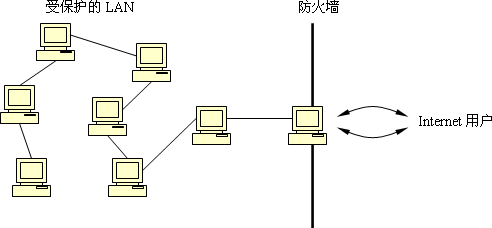
\includegraphics[scale=0.5]{network_firewall.png}
\caption{Firewall}
\label{network_firewall}
\end{figure}


防火墙会强制执行一个组织的访问控制策略(Access Control Policy),来执行接受和拒绝什么类型的网络通信。例如一个特定的组织可能只允许它的用户和外界以Email进行网络通信,拒绝其他任何通信方式,如站点访问等。另一个组织可能允许用户自由访问Internet,但不想让一般的Internet用户渗透到它的系统中或访问它的数据。组织的系统管理员将为他们的LAN设置防火墙,接受“可接受”类型的通信,拒绝其他类型的通信。实现这一点的方法有很多,最简单的一种是用端口号拒绝通信。例如,可建立防火墙,通过拒绝由端口23进入的所有通信,能够阻止LAN之外的用户创建对LAN之内机器的telnet连接。


更复杂的防火墙系统能维护有关流经它们的通信的状态的内部信息或存储数据本身,防火墙能够决定的通信状态越多,就越能保护它的用户。当然,这种安全是有代价的,有些防火墙会给网络通信带来明显的延迟。

不幸地是,很多微软的 windows 用户都意识不到其网络设置中常见的安全漏洞。下面是 Microsoft Windows 中常见的网络组件安装列表:

\begin{compactitem}
\item Microsoft 网络客户端
\item Microsoft 的文件和打印机网络共享
\item Internet 协议(TCP/IP )
\end{compactitem}

允许在 TCP/IP 上使用 NetBIOS,那么会面临一个安全问题:

\begin{compactitem}
\item 文件会被整个 Internet 共享
\item 用户的登录名、计算机名称以及工作组名称对其他人都是可见的
\end{compactitem}

而允许 TCP/IP 上的文件和打印机共享,也会面临安全问题:

\begin{compactitem}
\item 文件会被整个 Internet 共享
\end{compactitem}

没有连接任何网络的计算机也可能拥有危险的网络设置,这是由于一旦 Internet 被安装,网络设置就会发生改变。

上述的情况的解决方案是在网络连接属性中禁用 NetBIOS 协议和文件打印机共享,具体的操作方法会因不同的 windows 版本而略有不同。如果仍然需要在网络上共享打印机和文件,可以选择使用 NetBEUI 协议来代替 TCP/IP 协议。







\chapter{Network Address}

在通过计算机网络进行通信时,最终都是在与世界上某处的另一台计算机通信,因此Internet网络的地址必须精确到一台特定的机器,标识特定的机器以建立通信是一种相当复杂的机制。

主机名(Hostname)是Internet上的计算机的唯一标识,主机名通常是易读懂的单词,中间由点号分隔。例如:

\begin{lstlisting}[language=HTML]
matisse.csc.villanova.edu
condor.developcorp.com
theqiong.com
\end{lstlisting}


每个计算机必须有一个 IP 地址才能够连入因特网,每个 IP 包必须有一个地址才能够发送到另一台计算机。在处理Email地址和站点时,倾向于使用主机名,每个主机名对应一个IP地址,网络软件要把主机名翻译成对应的IP地址,便于计算机使用。

TCP/IP 使用 4 个数字来为计算机编址,每个计算机通常有一个唯一的 4 个十进制数的地址,中间由点号分隔,唯一的标识了Internet上的机器。例如:


\begin{lstlisting}[language=HTML]
205.39.145.18
193.133.20.4
\end{lstlisting}


整个Internet协议都是以32位(bit)的IP地址为基础的,也就是说TCP/IP 使用 32 个比特来编址,一个IP地址长为32位,IP地址中的每个数对应IP地址中的一个字节。

由于一个字节(8位)可以表示256种事物,所以IP地址中的数字的范围是0到255,即从00000000、00000001、00000010、00000011、00000100、00000101、00000110、00000111、00001000 ……直到 11111111,如下图所示:

\begin{figure}[!h]
\centering
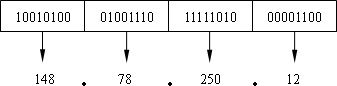
\includegraphics[scale=0.5]{network_ip_address.png}
\caption{IP地址}
\label{network_ip_address}
\end{figure}



虽然主机名和IP地址都是由点号分隔成几个部分,但是它们的每个部分之间不存在对应关系,整个主机名对应一个IP地址,而且IP地址一定有4个值,而主机名包含几部分是不确定的。

可以把IP地址分割成网络地址(Network Address),指定一个特定的网络和主机号,后者指定了网络中的一台特定机器。


如何分隔IP地址是由它表示的网络的类别决定的。不同大小的网络具有不同的网络类(A、B和C)。


A类网络把第一个字节作为网络地址,其他三个字节用作主机名。B类网络把前两个字节作为网络地址,后两个字节用作主机号,C类网络把前三个字节作为网络地址,最后一个字节用作主机号。

考虑一下采用这种寻址方法,每种网络的取值范围。A类网络比较少,但是每个网络中的主机较多。另一方面,C类网络很多,但每个网络中的主机很少。

大多数组织使用的是C类网络地址,A类和B类网络地址是为大型组织和ISP保留的。


\section{Domain Name}

主机名是由计算机名加域名构成的,例如,在主机名matisse.csc.villanova.edu中,matisse是计算机名,csc.villanova.edu是域名。

主机名中说明特定的组织或分组的部分叫做域名,域名由两个或多个部分组成,它们说明了计算机所属的组织或组织的一个子集。例如在这个例子中,matisse是Villanova大学的计算机系的一台计算机。

域名仅限于由特定组织控制的一组特定网络,而且不同组织中的计算机可以重名,因为从域名可以分辨出引用的是哪一台计算机。





域名中的最后一部分叫做顶级域名(Top-Level Domain,TLD),TLD声明了组织的类型或所属国家,下表列出了主要的顶级域名。

\begin{table}
\centering
\caption{主要的顶级域名}
\label{top_level_domain}
\begin{tabular}{|p{60pt}|p{60pt}|p{60pt}|p{60pt}|}
\hline
顶级域名		&用途		&	新顶级域名	& 用途\\
\hline
.com			&公司		& .biz			&商业\\
\hline
.net			&网络		&.info			&信息\\
\hline
.org			&非营利组织	&.pro			&专业\\
\hline
.edu			&教育部 		&.museum 		&博物馆\\
\hline
.int			&国际 		&.aero 			&航空业\\
\hline
.mil			&陆军 		&.coop			&合作团体\\
\hline
.gov			&政府 		&				&\\
\hline

\end{tabular}
\end{table}

每种域名用于一种特定类型的组织,例如.com用于商业组织,.edu用于大学和学院,美国以外的国家的组织采用国家代码作为顶级域名。下表列出了部分国家代码。

\begin{table}
\centering
\caption{部分国家代码}
\label{nation_code}
\begin{tabular}{|p{100pt}|p{100pt}|}
\hline
国家代码TLD	&国家\\
\hline
.au			&澳大利亚\\
\hline
.br			&巴西\\
\hline
.ca			&加拿大\\
\hline
.gr			&希腊\\
\hline
.in 			&印度\\
\hline
.ru 			&俄联邦\\
\hline
.uk 			&英国\\
\hline
\end{tabular}
\end{table}


最初,任何人或任何组织都可以注册自己的域名,只要这个名字还没被用到即可。

现在顶级域名(如.com和.edu)已经变得拥挤不堪了,已经为了缓解目前域名使用存在的问题,通过了新的顶级域名集合。

新的顶级域名注册制度使用新TLD的域名受到了限制,只有具有商标专用权的组织才能申请对应的域名。

域名注册的另一个来源是过期的域名。当注册了一个域名后,假设没有法律或商标方面的争议,那么只要付清费用(可以提前支付 10 年的费用),就可以自由地使用任意长的时间。




\section{Sub Domain Name}


大多数人们都没有意识到,但确实是每天都在使用着子域名。在Internet上可以见到很多子域名的例子:比如 store.apple.com 和 support.microsoft.com,最常见的 "www" 其实就是典型的子域名。

子域名可以在 DNS服务器上创建,并且不需要通过域名注册机构来进行注册。当然,在创建子域名之前,还是需要首先注册原始域名的,然后就可以请求网站主机提供商来创建子域名,也可以通过管理DNS服务器来创建。

某些提供商可能会为用户提供一个位于其域名之下的一个唯一的名称:www.theircompany.com/yourcompany/,但这并不是一个真实的域名,而是一个目录,而且应当尽量避免这样的情况。

这种 URL 的典型运用是通过 ISP 用于个人网站或免费网站,其实就是分享一个独立域名的方式,可为用户提供属于自己的地址。




\section{Domain Name System}

用于 TCP/IP 地址的名字被称为域名,域名系统(DNS,Domain Name System)主要用于把域名翻译成数字IP地址。

在DNS建立之前,斯坦福大学的一个研究小组负责维护一个文件主机表。每建立一个新主机名,斯坦福小组就把它添加到该表(每周两次),系统管理员会读取修改过的主机表,更新他们的域名服务器(把主机名翻译(解析)成IP地址的计算机)。

随着主机名数量的增长,只用一个表记录主机名已经不可行了,对于更新和分发信息来说,它不是一种实用的方法。1984年,网络工程师设计出了目前使用的复杂域名系统。


在全世界,数量庞大的 DNS 服务器被连入因特网,DNS已经从最初包括所有信息的单个文件发展成了把任务分配给几百万个域名服务器的分布式系统,其本身也演变成了一种分布式数据库,没有一个组织要负责更新主机名/IP映射。

DNS 服务器负责将域名翻译为 TCP/IP 地址,同时负责使用新的域名信息更新彼此的系统。当一个新的域名连同其 TCP/IP 地址一同注册后,全世界的 DNS 服务器都会对此信息进行更新。

现在,域名被称为是网站的唯一名称,当域名被注册后,就会被添加到大的域名注册商那里,连同与网站有关的信息——包括被保存在 DNS 服务器的 IP 信息,现在DNS服务器的功能包括负责向 Internet上的其他计算机通知有关你的域名和地址的信息。


在网络浏览器窗口或Email地址中指定了一个主机名时,浏览器或Email软件将给附近的域名服务器发送一个请求。如果这台服务器可以解析主机名,则进行解析,否则这台服务器将把这个请求转发给另一台域名服务器。如果第二台域名服务器也不能解析它,会继续转发这个请求,最终该请求到达一台能够解析它的服务器,或者因为解析时间太长而过期。



\chapter{WWW}

万维网的全名是World Wide Web,简称Web,与Internet相比,Web是个相对较新的概念,而且两者有着本质的不同。




从20世纪50年代开始,网络就用于连接计算机,这也是早期的Internet的雏形。虽然Internet已经用于通信多年了,但早期的通信几乎都是采用基于文本的Email和基本的文件交换实现的。



Web是与使用网络交换信息的软件结合在一起的分布式信息的基础设施,从而人们可以通过鼠标点击和图形界面操作,得到任何想要的资源。



WWW 是一张遍布全球的计算机网络,Web 中的所有计算机均可彼此相互通信,所有的计算机都使用被称为 HTTP 的通信标准。

Internet使通信成为了可能,而Web则使通信变得轻松、丰富和有趣。在Internet出现之后,直到20世纪90年代中期才出现了Web,从而使Internet普及到个人和家庭,也使Internet成为了商业的主要通信工具,自此以后,电子商务、电子支付、财务事项往来和小组管理变成了常见的在线活动,这也是Web对日常生活方式和商业模式的影响。

Web 信息存储于被称为网页(Web Page)的文档中,网页是存储于名为Web服务器的计算机中的文件。Unix 是首个(或最原始的)Web服务器操作系统,并以可靠性和稳定性而闻名。


读取网页的计算机可称为Web客户机,Web客户机通过名为Web浏览器的程序来查看页面。

网页中包括或引用各种数据,这些数据包括文本、图像、图形或程序。Web页还包含对其他Web页的链接(link),以便用户能够使用计算机鼠标在用户界面上跳转。

Web站点(Site)是一组相关的Web页,这组Web页通常是由个人或公司设计和控制的,Web站点的设计和实现技术多种多样。



在使用Web时,要“访问”一个Web站点,其实就是请求存储在远程Web服务器上的Web页,把它传输到本地计算机上以便浏览。

在Web服务器上,网页可作为 CGI 脚本来执行。CGI 脚本可在服务器上执行,来生成动态的交互性页面。大多数的 ISP 都会提供对 CGI 的某种程度的支持。并且许多都提供了使用 CGI 编写的预先安装的可运行的留言簿、页面计数器以及聊天/论坛解决方案。


所有的网页都含有供显示的指令,浏览器通过读取这些指令来显示页面,其中最常用的显示指令是 HTML 标签。只要客户机说明想要的信息,它们就会通过Web浏览器呈现在我们面前。



我们使用Web浏览器(Browser)在Web上通信,Web浏览器是处理Web页的请求并在它到达后将它显示出来的软件工具,例如Netscape Navigator、Internet Explorer、Mozilla Firefox、Apple Safari、Opera、Google Chrome等。对于网站开发人员来说,Web浏览器信息和统计数据的非常重要的。


浏览器可以通过一个请求 (request) 从Web服务器读取页面,其中请求是包含页面地址的标准 HTTP 请求,地址看上去类似这样:http://www.theqiong.com/index.html。


通过浏览器获取一个Web页的过程可以表示如下:

\begin{figure}[!h]
\centering
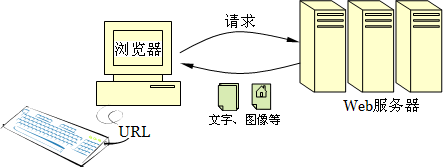
\includegraphics[scale=0.5]{network_browser.png}
\caption{通过浏览器获取一个Web页的过程}
\label{network_browser}
\end{figure}


被请求的Web页通常存储在另一台计算机上,用于响应Web请求的计算机就叫做Web服务器(Server)。Web页包含文本和其他独立的元素,比如图像。在请求Web页之后,所有与这个页面相关的元素都会被返回浏览器中。


在浏览器中,我们用Web地址说明我们想要的Web页,例如:www.villanova.com/academics.html

Web地址是统一资源地址(Uniform Resource Locator,URL)的核心部分,可以使用URL指定我们想要浏览的Web文档。URL唯一标识了存储在世界各处的Web页,而且URL的一部分是存储信息的计算机的主机名。



所有的 W3C 标准(自从1996年),包括 HTML、XHTML 和 XML 都定义了一个名为 Unicode (ISO 10646) 内部的内部字符集。

所有现代Web浏览器都在原生地使用此字符集,然而大多数在 internet 上传输的文档并没有使用这个 Unicode 字符集,因此Internet 客户(浏览器)与 Internet 服务器之间必须有一种在通信中一致使用字符集的方法。

对每个文档在用的字符集进行标记,对于提升网站的品质来说至关重要,推荐始终在 <head> 元素内 使用下面的的元元素:

\begin{lstlisting}[language=HTML]
<meta http-equiv="Content-Type" content="text/html;charset=utf-8" />
\end{lstlisting}

这里的charset是网页所使用的字符集,比如ISO-8859-1、UTF-8 或者 UTF-16。

类似 "04-03-02" 的日期格式在网页上可能被表示为2004年3月2日,或者2002年3月4日,亦或者2002年4月3日,因此国际标准化 (ISO) 为日期定义的国际标准格式是 "yyyy-mm-dd",yyyy 是年,mm 是月,dd 是日。


\section{Email}


POP(邮局协议)是一种用于发送和接收电子邮件的标准客户机/服务器协议。电子邮件会被接收并保存到internet 服务器上,直到用户通过某个客户段邮件程序(比如 Outlook 和 Foxmail)来收取信件。


IMAP 指的是 Internet 消息访问协议,这是另外一种用于发送和接收电子邮件的标准协议。

IMAP 在 POP 的基础上提供了一定的改进,即存储在 IMAP 服务器上的电子邮件可以由多台计算机处理,而无需在计算机间来回传输消息,而 POP 被设计为支持在一台单独的计算机上进行的邮件访问。


基于Web的电子邮件使用户通过Web浏览器就可以访问电子邮件。通过Web登陆到电子邮件帐户以后就可以发送和接收电子邮件了,能够从世界上的任何地方访问电子邮件是件很吸引人的事情。


\section{Search Engine}

Web搜索引擎是帮助用户找到其他站点的站点,比如Google和Yahoo!等。在搜索引擎中,用户通过输入单词或关键字(key word),说明你想要找的信息的类型,搜索引擎就会根据这些搜索相关信息,给用户提供一个有可能匹配检索要求的候选站点列表。

第一个因特网搜索工具叫做Archie,这是加拿大麦吉尔大学的计算机系学生在1990年开发的。Archie针对因特网上所有的匿名登录FTP站点设立了一个可供搜索和下载的数据库,这正是搜索引擎的雏形。

搜索引擎是通过检索具有上百万个站点的信息的数据库来生成候选站点列表的。好的搜索引擎会保持自己的数据库是最新的,而且具有匹配关键字和Web页内容的有效技术。有些搜索引擎只是以用户输入的关键字为依据,而有些则会尝试解释关键字的内涵,比如通过上下文匹配等。

大多数搜索引擎是通过用户输入的关键字与作为站点索引的一组关键字进行比较来确定搜索结果的。有些搜索引擎几乎把每个Web页上的每个单词都作为索引存入数据库的,只是除去“a”、“an”和“the”这样的常用单词。有些搜索引擎则只用Web页的部分内容作为索引,如文档的标题和副题等。有些索引技术区分大小写,有些则不区分。

关键字检索非常具有挑战性,因为自然语言(如英语)本身具有二义性,例如,术语hard cider(烈性苹果酒)、hard brick(坚硬的砖)、hard exam(很难的测验)和hard drive(磨损的道路)中的hard的意思都不同。如果提供了足够的关键字,搜索引擎能够正确地区分匹配站点的优先次序,但是在没有上下文的情况下,基本的关键字匹配是很有限的。

有些搜索引擎执行基于概念的搜索,即尝试判断所执行的搜索的上下文。如果它们运行的很好,返回的候选页会包含要检索的主题的相关内容,无论这个页面中的单词是否与查询中的关键词完全匹配。

执行基于概念的搜索的技术有几种,它们通常以复杂的语言理论为基础,这些技术的基本前提是分类,即对比相近的单词。例如,在医学领域中,心脏这个词可能与动脉、胆固醇和血这些词相近。

基于概念的搜索引擎比关键字检索复杂的多,而且现在基于概念的搜索技术还很不完善,这种技术在搜索引擎发展中很有潜力。



\section{IM}



即时消息(Instant Message)应用程序可能是目前最受欢迎的Web程序,它给了Web另一种交互方式。使用这些IM程序,可以实时地给朋友或工作伙伴发送消息,进行在线交流。如果发送者和接收者同时运行了即时消息程序,那么消息一到达就会立刻提醒或展示在用户面前,这样两个人就能够进行在线交流。现在领先的IM应用程序包括America Online(AOL)Instant Messenger(AIM)和Tencent QQ。

IM应用程序发展到现在,可以允许用户定制联系人列表,设置默认的答复,除了文本外,还可以发送标准的图形或订制的图形,IM模式已经成为了许多用户的标准通信方式,现在IM程序已经发展成了具有图像和视频等应用。

大多数IM应用程序使用专有的协议,规定发送信息的格式和结构,比如AIM的协议也是专有的,但并不限于AOL用户才能使用,这也促进了AOL的流行。

IM应用程序虽然方便,但却并不安全,通过各种IM协议发送的消息并没有加密,可能会被网络通途中的中间点截获,未加密的Email也同样不安全。

\chapter{W3C}

万维网联盟(World Wide Web Consortium,W3C)创立了 WWW 标准,W3C 的使命是通过发展规范、指导方针、软件以及工具,来尽展万维网潜能。

“web 蕴藏的梦想是一个可在其中通过分享信息而进行通信的公共信息空间。”

\begin{flushright}
——Tim Berners-Lee,万维网的发明人,W3C 的主任及创立者
\end{flushright}

万维网(World Wide Web)是作为欧洲核子研究组织的一个项目发展起来的,这那里 Tim Berners-Lee 开发出万维网的雏形。

W3C 在 1994 年被创建的目的是,为了完成麻省理工学院(MIT)与欧洲粒子物理研究所(CERN)之间的协同工作,并得到了美国国防部高级研究计划局(DARPA)和欧洲委员会(European Commission)的支持。现在,W3C是一个致力于“尽展万维网潜能”的国际性联盟。

\begin{compactitem}
\item W3C 指万维网联盟(World Wide Web Consortium)
\item W3C 被创建于 1994 年 10 月
\item W3C 由 Tim Berners-Lee 创立
\item W3C 由Web的发明人创立
\item W3C 以会员机构的形式进行组织
\item W3C 致力于对Web进行标准化
\item W3C 创建并维护了 WWW 标准
\item W3C 标准被称为 W3C 推荐标准(W3C Recommendations)
\end{compactitem}

W3C 致力于实现所有的用户都能够对Web加以利用(不论其文化教育背景、能力、财力以及其身体残疾),其最重要的工作是发展Web规范(称为推荐,Recommendations),这些规范描述了Web通信协议(比如 HTML 和 XML)和其他构建模块的“推荐标准”,最重要的 W3C 标准包括:

\begin{compactitem}
\item HTML
\item XHTML
\item CSS
\item XML
\item XSL
\item DOM
\end{compactitem}

每项 W3C 推荐的发展是通过由会员和受邀专家组成的工作组来完成的。工作组的经费来自公司和其他组织,并会创建一个工作草案,最后是一份提议推荐。一般来说,为了获得正式的批准,推荐都会被提交给 W3C 会员和主任。

W3C 同时与其他标准化组织协同工作,比如 Internet 工程工作小组(Internet Engineering Task Force)、无线应用协议(WAP)以及 Unicode 联盟(Unicode Consortium)。

目前,W3C由美国麻省理工学院计算机科学和人工智能实验室 (MIT CSAIL),总部位于法国的欧洲信息数学研究联盟 (ERCIM) 和日本的庆应大学(Keio University)联合运作,并且在世界范围内拥有分支办事处。

正因为 Web 是如此的重要(不论在其影响范围还是在投资方面),以至于不应由任何一家单独的组织来对它的未来进行控制,因此 W3C 扮演者一个会员组织的角色:

\begin{compactitem}
\item IBM
\item Microsoft
\item America Online
\item Apple
\item Adobe
\item Macromedia
\item Sun Microsystems
\item ...
\end{compactitem}

W3C 的会员包括了软件开发商、内容提供商、企业用户、通信公司、研究机构、研究实验室、标准化团体以及政府。

W3C 国际化活动的目标是,在 W3C 内部以及与其他组织一起,建议并调整任何技术、协定、指导方针和活动,使得在不同的语言、脚本和文化范畴内更易在全球范围内使用 W3C 技术。


W3C 中国办事处成立于 2006 年 4 月 1 日。现设址于北京航空航天大学(BUAA),由北京航空航天大学计算机学院计算机新技术研究所负责日常运营工作。

W3C中国办事处致力于促进国内外万维网标准领域信息沟通互动,为国内企业、高校、及科研机构参与国际信息技术标准化的研究、集成和推广提供更好的服务。

W3C 在中国的会员包括:

\begin{compactitem}
\item 北京航空航天大学
\item 北京工业大学
\item 中国电子技术标准化研究所
\item 广州中间件研究中心
\item 安徽中科大讯飞信息科技有限公司
\item 倍多科技
\item 太原理工大学
\item ISTIC 中国科学技术信息研究所
\item Uncover China
\item Monotype Imaging Inc.
\item Industrial Technology Research Institute (ITRI) Taiwan
\item 香港特别行政区政府科技资讯总编办公室 (OGCIO)
\end{compactitem}

2009 年 11 月 14 日,W3C 及其中国办事处与全国各地关注 W3C 的志愿者团体和个人相聚北京,共议 W3C 中国社区建设计划启动事宜。

\section{W3C Procedure}

W3C 的标准化程序分为 7 个不同的步骤。在 W3C 发布某个新标准的过程中,规范是通过下面的严格程序由一个简单的理念逐步确立为推荐标准的:

\begin{compactitem}
\item W3C 收到一份提交
\item 由 W3C 发布一份记录
\item 由 W3C 创建一个工作组
\item 由 W3C 发布一份工作草案
\item 由 W3C 发布一份候选的推荐
\item 由 W3C 发布一份被提议的推荐
\item 由 W3C 发布推荐
\end{compactitem}

\begin{compactenum}
\item W3C 提交 (W3C Submissions)

任何 W3C 的成员都可向联盟提交希望成为 Web 标准的某项建议(案)。大多数W3C推荐都发源于向联盟做出的某个提交。

如果某项提交在 W3C 的工作领域(或宪章)内,那么 W3C 将决定是否启动对该项提议的改进工作。

\item W3C 记录 (W3C Notes)

通常,一项对 W3C 的提交会成为一份记录。记录是对作为一份公共文档来提炼的一项提议的描述。

W3C 仅把记录用户讨论。记录的发布并不代表对其的认可。记录的内容是由提交此记录的会员来编辑的,而不是 W3C。记录可在任何时间被更新、替换或废弃。记录的发布也不表明 W3C 已启动与此记录相关的任何工作。

\item W3C 工作组 (W3C Working Groups)

当某项提交被 W3C 承认,一个工作组就会成立,其中包括会员和其他有兴趣的团体。

工作组通常会定义一个时间表,并发布有关被提议标准的工作草案。

\item W3C 工作草案 (W3C Working Drafts)

W3C 工作草案通常会被发布于 W3C 的网站上,连同对公共注解的邀请。

工作草案会说明进行中的工作,但不应被用作任何参考材料。其内容可在任何时间被更新、替换或废弃。

\item W3C 候选推荐 (W3C Candidate Recommendations)

某些规范会比其他规范更复杂,并可能需要来自会员和软件开发商的更多的经费、更多时间以及更多测试。有时,这些规范会作为候选的推荐来发布。

候选的推荐也是一种“正在进行的工作”,同样不应被用作参考材料。此文档可在任何时间被更新、替换或废弃。

\item W3C 提议推荐 (W3C Proposed Recommendations)

提议的推荐意味着工作组中工作的最后阶段。

提议推荐也是一种“正在进行的工作”。此文档可在任何时间被更新、替换或废弃。不过即使它不意味着 W3C 的任何官方的认可,在极多的情况下,提议的推荐无论在内容还是时间上都已接近于最后的推荐。

\item W3C 推荐 (W3C Recommendations)

W3C 推荐已经通过了 W3C 会员们的评审,并得到了 W3C 主任的正式批准。

W3C 推荐是一份稳定的文档,并可被用作参考材料。

\end{compactenum}





\section{W3C HTML}

HTML 2.0 是 1996 年由 Internet 工程工作小组的 HTML 工作组开发的。现在HTML 2.0 已经是过时的 HTML 版本。目前在市场上可以找到的浏览器都依赖于更新版本的 HTML。对于一位 WEB 开发者而言,没有任何必要需要 HTML 2.0 标准。

HTML 3.2 作为 W3C 标准发布于 1997 年 1 月 14 日。HTML 3.2 向 HTML 2.0 标准添加了被广泛运用的特性,诸如字体、表格、applets、围绕图像的文本流,上标和下标,其中被添加到 1997 年 HTML 3.2 标准的元素之一 - <font> 标签 - 为 HTML 内容和呈现的分离这个重要的任务带来了不必要的麻烦。

作为一项 W3C 推荐,HTML 4.0 被发布于 1997 年 12 月 18 日,HTML 4.0 最重要的特性是引入了样式表(CSS)。而仅仅进行了一些编辑修正的第二个版本发布于 1998 年 4 月 24 日。



作为一项 W3C 推荐,HTML 4.01 发布于 1999 年 12 月 24 日,HTML 4.01 是对 HTML 4.0 的一次较小的更新,对后者进行了修正和漏洞修复。

W3C 不会继续发展 HTML,未来 W3C 的工作会集中在 XHTML 上。作为一项 W3C 推荐,XHTML 1.0 发布于 2000 年 1 月 20 日。

XHTML 1.0 使用 XML 对 HTML 4.01 进行了重新地表示。



W3C 于 2008 年 1 月 22 日发布 HTML 5 工作草案。

HTML 5 中的新特性包括了嵌入音频、视频和图形的功能,客户端数据存储,以及交互式文档。

HTML 5 还包含了新的元素,比如:<nav>, <header>, <footer> 以及 <figure> 等等。

通过制定如何处理所有 HTML 元素以及如何从错误中恢复的精确规则,HTML 5 改进了互操作性,并减少了开发成本。

HTML 5 工作组包括:AOL, Apple, Google, IBM, Microsoft, Mozilla, Nokia, Opera, 以及数百个其他的供应商。

\begin{longtable}{|m{90pt}|m{90pt}|m{180pt}|}
%head
\multicolumn{3}{r}{}
\tabularnewline\hline
规范	& 草案/提议	&推荐
\endhead
%endhead

%firsthead
\caption{W3C HTML 规范和时间线}\\
\hline
规范	& 草案/提议	&推荐
\endfirsthead
%endhead

%foot
\multicolumn{3}{r}{}
\endfoot
%endfoot

%lastfoot
\endlastfoot
%endlastfoot
\hline
HTML 3.2	&&1997 年 1 月 14 日\\
\hline
HTML 4.0	&&1998 年 5 月 24 日\\
\hline
HTML 4.01	&&1999 年 12 月 24 日\\
\hline
HTML 5		&&2010 年 6 月 24 日(最新草案)\\
\hline

\end{longtable}




\section{W3C XHTML}

作为一项 W3C 推荐,XHTML 1.0 发布于 2000 年 1 月 26 日,XHTML 1.0 是使用 XML 对 HTML 4.01 进行的重新表示。

作为一项 W3C 推荐,XHTML 1.0 第二版发布于 2002 年 8 月 1 日。它不是一个新的版本,而是一次更新和漏洞修复。

XHTML 1.0 是自 1997 年以来对 HTML 的第一次主要的改变,同时也是在向更广泛的用户代理提供更丰富网页的道路上迈出的非常重要的一步,这些用户代理(代理)包括桌面电脑、移动设备和手机等等。

XHTML 是一项可从 HTML 4.01 平稳迁移的 XML 应用。W3C 把 HTML 4.01 重构为 XML 的第一个步骤,导致了 XHTML 1.0 的诞生。XHTML 1.0 依赖于 HTML 4.01 标签所提供的语义。

下一步是把 XHTML 模块化为更小的元素集合,使得 XHTML 和其他标记语言(比如矢量图形和多媒体)的结合更加容易。

同时,XHTML 的模块化还可以减少开发费用,改善与其它应用程序(比如数据库)的协同,更易与不同的用户代理(浏览器)进行通信,以及 HTML 和不同 XML 标准之间更纯净的整合。


XHTML 1.1 是一门严格的语言,且XHTML 1.1 不能向后兼容 HTML 4,小型设备(比如移动电话)也无法支持 XHTML 的全部功能。XHTML 1.1 将规范划分为具备有限功能的模型,小型浏览器只能通过支持选定的模型来减低其复杂性(不过一旦选定某个模型,就必须支持其全部特性)。

XHTML Basic 是 XHTML 1.1 的小型子集,它仅包含基本的 XHTML 特性,比如文本结构、图像、基本的标单以及基本的表格。它是为小型浏览器设计的(比如在手持设备中)。

正是由于 XHTML 中对 W3C 文档对象模型级别 2 的支持,事件处理器就可以依附在 XHTML 元素上,这样父元素就可以在子元素之前或之后来处理事件。

XHTML-Print 是 XHTML 1.1 (模块化的 XHTML) 的一部分,它被设计用于移动设备和廉价的打印机,这些设备通常可在没有打印缓存和为设备定制的打印驱动的情况下,将一张页面从头到尾打印出来。

XForms 是 HTML 表单的继任者,提供一种更完善且独立于呈现的 Web交 互事务处理方式。通过 XHTML 表单,用户可以访问某张页面,向页面添加信息,然后向Web服务器提交页面。

XForms被设计为与 XHTML 进行整合,我们期望未来的电子商务应用程序会需要需要 XForms。

XHTML 2.0 是下一代的标记语言。其功能性预计和 XHTML 1.1 很相似,但是可能被变更来遵守 XML 标准的要求,比如 XML Linking 和 XML Schema。

XHTML 1.0 的模块化是通过使用 XML DTD (Document Type Definition) 来实现的,而XHTML 2.0 的模块化是通过使用 XML Schemas 来实现的。

XLink 是在 XML 文档中创建超链接的一门语言。XLink 与 HTML 链接很相似 - 但是更加强有力地支持简单链接(比如 HTML)和扩展链接(用于把多项资源链接到一起)。

HLink 是对 XLink 的扩展,HLink 增加了一项能力,可规定在 XHTML 中元素哪项元素可表示超链接,并规定如何对超链接进行遍历。

\begin{longtable}{|p{180pt}|p{90pt}|p{90pt}|}
%head
\multicolumn{3}{r}{}
\tabularnewline\hline
规范	& 草案/提议	&推荐
\endhead
%endhead

%firsthead
\caption{W3C XHTML 规范和时间线}\\
\hline
规范	& 草案/提议	&推荐
\endfirsthead
%endhead

%foot
\multicolumn{3}{r}{}
\endfoot
%endfoot

%lastfoot
\endlastfoot
%endlastfoot
\hline
XHTML 1.0	 				&&2000 年 1 月 26 日\\
\hline
XHTML 1.0 修订版	 		&&2002 年 8 月 1 日\\
\hline
XHTML 1.1	 				&&2001 年 5 月 31 日\\
\hline
XHTML Modules	 			&&2001 年 4 月 10 日\\
\hline
XHTML Modules 1.1			&&2008 年 10 月 8 日\\
\hline
XHTML Basic	 			&&2000 年 12 月 19 日\\
\hline
XHTML Basic 1.1			&&2008 年 7 月 29 日\\
\hline
XHTML Events	 			&&2003 年 10 月 14 日\\
\hline
XHTML Print	 			&&2006 年 9 月 20 日\\
\hline
XHTML Media Types (SE)	&2009 年 1 月 16 日	 &\\
\hline
XHTML 2.0					&2006 年 7 月 26 日	 &\\
\hline
XForms 1.0	 				&&2003 年 10 月 14 日\\
\hline
XForms 1.0 (Third Edition)	&&2007 年 10 月 29 日\\
\hline
XForms 1.1					&2009 年 10 月 20 日	 &\\
\hline
XLink	 					&&2001 年 6 月 27 日\\
\hline
HLink						&2002 年 9 月 13 日	 &\\
\hline
\end{longtable}

\section{W3C XML}

XML 被设计用来描述、存储、传送及交换数据。


作为一项 W3C 推荐,XML 1.0 发布于 1998 年 2 月 10 日。

作为一项 W3C 推荐,XML 1.0 (SE) 发布于 2000 年 10 月 6 日。第二版仅仅是在合并第一版的勘误表的基础上进行的修正(漏洞修复),随后的第三版也仅仅是在合并第一版和第二版的勘误表的基础上进行的修正(漏洞修复)。

作为一份工作草案,XML 1.1 发布于2001 年 12 月 13 日,并作为一项候选推荐发布于2002年10月15日。XML 1.1 允许在名称中使用几乎所有的 Unicode 字符。

\begin{compactitem}
\item XML 命名空间(Namespaces)可规定一种方法,通过与 URI 引用相关联的方式,来定义在 XML 中使用的元素和属性名称。
\item XML Linking 语言 (XLink),允许您向XML文档中插入链接。
\item XML Pointer 语言 (XPointer),允许将地址链接到 XML 文档的具体部分。
\item XML Base 是一种用于对外部 XML 资源进行默认引用的标准。(与 HTML 中的 <base> 类似)。
\item XInclude 是一种使用元素、属性以及 URI 引用来合并 XML 文档的机制。
\end{compactitem}

\begin{longtable}{|p{180pt}|p{90pt}|p{90pt}|}
%head
\multicolumn{3}{r}{}
\tabularnewline\hline
规范	& 草案/提议	&推荐
\endhead
%endhead

%firsthead
\caption{W3C XML 规范和时间线}\\
\hline
规范	& 草案/提议	&推荐
\endfirsthead
%endhead

%foot
\multicolumn{3}{r}{}
\endfoot
%endfoot

%lastfoot
\endlastfoot
%endlastfoot
\hline
XML 1.0	 				&&1998 年 2 月 10 日\\
\hline
XML 1.0 (2.Ed)	 			&&2000 年 10 月 6 日\\
\hline
XML 1.0 (3.Ed)	 			&&2004 年 2 月 4 日\\
\hline
XML 1.1	 				&&2004 月 2 月 4 日\\
\hline
XML 1.1 (2.Ed)	 			&&2006 年 8 月 16 日\\
\hline
XML 1.0 Namespaces		&&	 	1999 年 1 月 14 日\\
\hline
XML 1.0 Namespaces SE 	&&	 	2004 年 3 月 4 日\\
\hline
XML 1.1 Namespaces		&& 	2004 年 3 月 4 日\\
\hline
XML 1.1 Namespaces SE 	&&	 	2006 年 8 月 16 日\\
\hline
XML Infoset	 				&&2001 年 10 月 24 日\\
\hline
XML Infoset (2.Ed)	 		&&2004 年 2 月 4 日\\
\hline
XML Base	 				&&2001 年 6 月 27 日\\
\hline
XLink 1.0	 				&&2001 年 6 月 27 日\\
\hline
XPointer Framework		&&	2003 年 3 月 25 日\\
\hline
XPointer element() scheme	&& 	2003 年 3 月 25 日\\
\hline
XPointer xmlns() scheme	&& 	2003 年 3 月 25 日\\
\hline
XInclude 1.0	 			&&2004 年 12 月 20 日\\
\hline
XInclude 1.0 SE	 			&&2006 年 11 月 15 日\\
\hline
XML Processing Model		&2004 年 4 月 5 日	 &\\
\hline
XMLHttpRequest Object		&2010 年 8 月 3 日	 &\\
\hline
\end{longtable}


\section{W3C CSS}

CSS 是一种向网页添加样式的机制,用于描述文档如何被显示、发音或打印。

作为一项 W3C 推荐,CSS1 发布于 1996 年 12 月 17 日。1999 年 1 月 11 日,此推荐被重新修订。

作为一项 W3C 推荐,CSS2 发布于 1999 年 1 月 11 日。CSS2 添加了对媒介(打印机和听觉设备)和可下载字体的支持。

CSS3 计划将 CSS 划分为更小的模块。

\begin{longtable}{|p{180pt}|p{90pt}|p{90pt}|}
%head
\multicolumn{3}{r}{}
\tabularnewline\hline
规范	& 草案/提议	&推荐
\endhead
%endhead

%firsthead
\caption{W3C CSS 规范和时间线}\\
\hline
规范	& 草案/提议	&推荐
\endfirsthead
%endhead

%foot
\multicolumn{3}{r}{}
\endfoot
%endfoot

%lastfoot
\endlastfoot
%endlastfoot
\hline
CSS 1	 			&&1996 年 12 月 17 日\\
\hline
CSS 1 (Revised)	 	&&1999 年 1 月 11 日\\
\hline
CSS 2	 			&&1998 年 5 月 12 日\\
\hline
CSS 2.1				&2007 年 7 月 19 日	 &\\
\hline
CSS 2 Mobile		&2007 年 10 月 19 日	 &\\
\hline
CSS 2 TV			&2003 年 5 月 14 日	 &\\
\hline
CSS 2 Print			&2006 年 10 月 13 日	 &\\
\hline
CSS 3				&2001 年 5 月 23 日	 &\\
\hline
CSS 3 Namespace	&2006 年 8 月 28 日	 &\\
\hline
CSS 3 User Interface&	2004 年 5 月 11 日	 &\\
\hline
CSS 3 Selectors		&2005 年 12 月 15 日	 &\\
\hline
CSS 3 Fonts		&2002 年 8 月 2 日	 &\\
\hline
CSS 3 Web Fonts	&2002 年 8 月 2 日	 &\\
\hline
CSS 3 Colors		&2003 年 5 月 14 日	 &\\
\hline
CSS 3 TV			&2003 年 5 月 14 日	 &\\
\hline
CSS 3 Backgrounds and borders	&2005 年 2 月 16 日	 &\\
\hline
CSS 3 Text			&2007 年 3 月 6 日	 &\\
\hline
CSS 3 Lists			&2002 年 11 月 7 日	 &\\
\hline
CSS 3 Line			&2002 年 5 月 15 日	 &\\
\hline
CSS 3 Box model	&2007 年 8 月 9 日	 &\\
\hline
CSS 3 Multi column	&2007 年 6 月 6 日	 &\\
\hline
CSS 3 Ruby			&2003 年 5 月 14 日	 &\\
\hline
CSS 3 Border		&2005 年 3 月 16 日	 &\\
\hline
CSS 3 Speech		&2004 年 12 月 16 日	 &\\
\hline
CSS 3 Paged Media (PM)	 &2006 年 10 月 10 日	 &\\
\hline
CSS 3 Generated PM	&2007 年 5 月 4 日	 &\\
\hline
CSS 3 Print			&2006 年 10 月 13 日	 &\\
\hline
CSS 3 Values		&2006 年 9 月 19 日	 &\\
\hline
CSS 3 Cascade		&2005 年 12 月 15 日	 &\\
\hline
CSS 3 Template Layout	&2009 年 4 月 2 日	 &\\
\hline
CSS 3 Media Queries	&2009 年 9 月 15 日	 &\\
\hline


\end{longtable}


\section{W3C XSL}


XSL 语言包括三部分:XSLT、XPath 以及 XSL 格式化对象。


作为一项 W3C 推荐标准,XSL 1.0 作为一门表达样式表的语言被发布于 2001 年 10 月 15 日。它由三部分组成:XSLT、XPath 以及 XSL 格式化对象。

XSLT 1.0于 1 999年11月16日成为 W3C 推荐标准。XSLT 是一门用于把 XML 文档转换为其他 XML 文档的语言。


XSLT 2.0于 2007 年 1 月 23 日成为 W3C 推荐标准。


XSL-FO (XSL 格式化对象)是一个用于规定格式化语义的词汇表。

格式化指的是把XSL转换的结果转变为适合阅读器或收听器的过程。虽然不存在针对 XSL 格式化对象的独立 W3C 文档,但是还是可以在 XSL 1.0 推荐标准中找到相关的描述。

\begin{longtable}{|p{180pt}|p{90pt}|p{90pt}|}
%head
\multicolumn{3}{r}{}
\tabularnewline\hline
规范	& 草案/提议	&推荐
\endhead
%endhead

%firsthead
\caption{W3C XSL 规范和时间线}\\
\hline
规范	& 草案/提议	&推荐
\endfirsthead
%endhead

%foot
\multicolumn{3}{r}{}
\endfoot
%endfoot

%lastfoot
\endlastfoot
%endlastfoot
\hline
XSL 1.0 (XSL-FO)	 	&&2001 年 10 月 15 日\\
\hline
XSL 1.1	 				&&2006 年 12 月 5 日\\
\hline
XSLT 1.0	 			&&1999 年 11 月 16 日\\
\hline
XSLT 1.1				&2001 年 8 月 24 日	&\\
\hline 
XSLT 2.0 Requirements	&2001 年 2 月 14 日	&\\
\hline 
XSLT 2.0	 			&&2007 年 1 月 23 日\\
\hline

\end{longtable}


\section{W3C XML Schema}

XML Schema 是基于 XML 的 DTD 替代物,XML Schema 对应用程序、文档结构、属性和数据类型有着更良好的支持。




XML 1.0 支持可定义文档结构的 DTD,未来的 XML 版本有赖于 XML Schema 来定义 XML 文档的类型。


\begin{compactitem}
\item XML Schema 的结构(XML Schema Structure)规定了 XML Schema 的定义语言。
\item XML Schema 的数据类型为 XML 规定了可扩展的数据类型。
\end{compactitem}


\begin{longtable}{|p{180pt}|p{90pt}|p{90pt}|}
%head
\multicolumn{3}{r}{}
\tabularnewline\hline
规范	& 草案/提议	&推荐
\endhead
%endhead

%firsthead
\caption{W3C XML Schema 规范和时间线}\\
\hline
规范	& 草案/提议	&推荐
\endfirsthead
%endhead

%foot
\multicolumn{3}{r}{}
\endfoot
%endfoot

%lastfoot
\endlastfoot
%endlastfoot
\hline
XML Schema	 			&&2001 年 5 月 2 日\\
\hline
XML Schema Structures	 	&&2001 年 5 月 2 日\\
\hline
XML Schema Datatypes	 	&&2001 年 5 月 2 日\\
\hline
XML Schema (2.Ed)	 		&&2004 年 10 月 28 日\\
\hline
XML Schema Structures (2.Ed)&&	 	2004 年 10 月 28 日\\
\hline
XML Schema Datatypes (2.Ed)&&	 	2004 年 10 月 28 日\\
\hline
XML Schema Component Designators&	2008 年 11 月 17 日&\\
\hline	 
XML Schema 1.1: Structures	 	&&2009 年 4 月 30 日\\
\hline
XML Schema 1.1: Datatypes	 	&&2009 年 4 月 30 日\\
\hline

\end{longtable}


\section{W3C XPath}



XPath 是一门用于选取 XML 文档的部件的语言,它被设计为供 XSLT、XQuery 以及 XPointer 使用。


XPath 1.0 于 1999 年 11 月 16 日成为 W3C 推荐标准。


XPath 2.0 于 2007 年 1 月 23 日成为 W3C 推荐标准,它是一门由 XPath 1.0 和 XQuery 衍生而来的语言。

XPath 2.0 和 XQuery 1.0 的产生是同源的,它们拥有不少相同的语法,而且不少文本也是一致的。




\begin{longtable}{|p{180pt}|p{90pt}|p{90pt}|}
%head
\multicolumn{3}{r}{}
\tabularnewline\hline
规范	& 草案/提议	&推荐
\endhead
%endhead

%firsthead
\caption{W3C XPath 规范和时间线}\\
\hline
规范	& 草案/提议	&推荐
\endfirsthead
%endhead

%foot
\multicolumn{3}{r}{}
\endfoot
%endfoot

%lastfoot
\endlastfoot
%endlastfoot
\hline
XPath 1.0	 			&&1999 年 11 月 16 日\\
\hline
XPath 2.0 Requirements	&2005 年 6 月 3 日	 &\\
\hline
XPath 2.0 Language	 	&&2007 年 1 月 23 日\\
\hline
XPath 2.0 Functions	 	&&2007 年 1 月 23 日\\
\hline
XPath 2.0 Data Model	&& 	2007 年 1 月 23 日\\
\hline
XPath 2.0 Semantics	&& 	2007 年 1 月 23 日\\
\hline
XPointer				&2002 年 8 月 16 日	 &\\
\hline
\end{longtable}


\section{W3C XQuery}

XQuery 是一门用于从 XML 文档中提取数据的语言,它是支持从 XML 文档提取数据的查询工具。

\begin{longtable}{|p{180pt}|p{90pt}|p{90pt}|}
%head
\multicolumn{3}{r}{}
\tabularnewline\hline
规范	& 草案/提议	&推荐
\endhead
%endhead

%firsthead
\caption{W3C XQuery 规范和时间线}\\
\hline
规范	& 草案/提议	&推荐
\endfirsthead
%endhead

%foot
\multicolumn{3}{r}{}
\endfoot
%endfoot

%lastfoot
\endlastfoot
%endlastfoot
\hline
XQuery Requirements	&2007 年 3 月 23 日	 &\\
\hline
XQuery Use Cases		&2007 年 3 月 23 日	 &\\
\hline
XQuery 1.0	 			&&2007 年 1 月 23 日\\
\hline
XQuery 1.0 Functions	&& 	2007 年 1 月 23 日\\
\hline
XQuery 1.0 Data Model	&& 	2007 年 1 月 23 日\\
\hline
XQuery 1.0 Semantics	&& 	2007 年 1 月 23 日\\
\hline
XQueryX	 			&&2007 年 1 月 23 日\\
\hline
XQuery 1.1 Requirements&	2007 年 3 月 23 日	 &\\
\hline
XQuery 1.1 Use Cases	&2008 年 12 月 3 日	 &\\
\hline
XQuery 1.1				&2008 年 12 月 3 日	 &\\
\hline
\end{longtable}




\section{W3C DOM}


文档对象模型 (DOM) 是一个平台,一个中立于语言的应用程序编程接口 (API),允许程序访问并更改文档的内容、结构和样式。


DOM 级别 0 不是 W3C 规范。而仅仅是对在 Netscape Navigator 3.0 和 Microsoft Internet Explorer 3.0 中的等价功能性的一种定义。W3C 的 DOM 级别 1 就是建立于此功能性之上。

DOM 发展过程中的关键角色有:ArborText、IBM、Inso EPS、JavaSoft、Microsoft、Netscape、Novell、the Object Management Group、SoftQuad、Sun Microsystems 以及 Texcel。



DOM 级别 1 于 1998 年 10 月 1 日成为 W3C 推荐标准,第二版的工作草案在 2000 年 9 月 29 日。

DOM 级别 1 专注于 HTML 和 XML 文档模型。它含有文档导航和处理功能。

DOM 级别 2 对 DOM 级别 1 添加了样式表对象模型,并定义了操作附于文档之上的样式信息的功能性。DOM 级别 2 同时还定义了一个事件模型,并提供了对 XML 命名空间的支持。

作为一项 W3C 推荐标准,DOM 级别 2 规范发布于 2000 年 11 月 13 日。

\begin{compactitem}
\item DOM Level 2 核心

DOM Level 2 核心 规定了访问和更改文档内容及结构的一个 API,此 API 同时包含用于 XML 的接口。

\item DOM Level 2 HTML

DOM Level 2 HTML 规定了操作 HTML 文档结构和内容的 API。(这部分规范仍然是工作草案)

\item DOM Level 2 Views

DOM Level 2 规定了对文档视图进行访问和更改的 API。视图是与原文档相关联的表现形式或某种备用的表现形式。

\item DOM Level 2 Style

DOM Level 2 Style 规定了动态访问及更改内容样式表的 API。

\item DOM Level 2 Events

DOM Level 2 Events 规定了访问文档事件的 API。

\item DOM Level 2 Traversal-Range

DOM Level 2 Traversal-Range 规定了动态遍历和识别文档中内容范围的 API。

\end{compactitem}


DOM Level 3 规定了内容模型 (DTD 和 Schemas) 和文档验证。同时规定了文档加载和保存、文档查看、文档格式化和关键事件。DOM Level 3 建立于 DOM Core Level 2 之上。

DOM Requirements 文档已经为 Level 3 requirements 进行了更新,并于 2000 年 4 月 12 日发布为工作草案。


下面的 DOM Level 3 工作草案发布于 2000 年 9 月 1 日:

\begin{compactitem}
\item DOM Level 3 Core

DOM Level 3 Core 规定了访问和更改文档内容、结构及样式的一个 API。

\item DOM Level 3 Events

通过增加新的接口和新的事件集,DOM Level 3 Events API 对 Level 2 Event API 的功能进行了扩展。

\item DOM Level 3 Load and Save

DOM Level 3 Content Model 规定了用于内容加载和保存、内容模型 (DTD and Schemas) 和文档验证支持的 API。

\item DOM Level 3 Views and Formatting

DOM Level 3 Views 规定了对文档视图进行访问和更改的 API。视图是与原文档相关联的表现形式或某种备用的表现形式。

\end{compactitem}

\begin{longtable}{|p{180pt}|p{90pt}|p{90pt}|}
%head
\multicolumn{3}{r}{}
\tabularnewline\hline
规范	& 草案/提议	&推荐
\endhead
%endhead

%firsthead
\caption{W3C DOM 规范和时间线}\\
\hline
规范	& 草案/提议	&推荐
\endfirsthead
%endhead

%foot
\multicolumn{3}{r}{}
\endfoot
%endfoot

%lastfoot
\endlastfoot
%endlastfoot
\hline
DOM Level 1	 		&&1998 年 10 月 1 日\\
\hline
DOM Level 1 (SE)		&2000 年 9 月 29 日	 &\\
\hline
DOM Level 2 Core	 	&&2000 年 11 月 13 日\\
\hline
DOM Level 2 HTML	 	&&2003 年 1 月 9 日\\
\hline
DOM Level 2 Views	 	&&2000 年 11 月 13 日\\
\hline
DOM Level 2 Style	 	&&2000 年 11 月 13 日\\
\hline
DOM Level 2 Events	 	&&2000 年 11 月 13 日\\
\hline
DOM Level 2 Traversal-Range&&	 	2000 年 11 月 13 日\\
\hline
DOM Level 3 Requirements	&2004 年 2 月 26 日	 &\\
\hline
DOM Level 3 Core	 		&&2004 年 4 月 7 日\\
\hline
DOM Level 3 Events			&2007 年 12 月 21 日	 &\\
\hline
DOM Level 3 Load and Save	&& 	2004 年 4 月 7 日\\
\hline
DOM Level 3 Validation	 	&&2004 年 1 月 27 日\\
\hline
DOM Level 3 XPath			&2004 年 2 月 26 日	 &\\
\hline
DOM Level 3 Views			&2004 年 2 月 26 日	 &\\
\hline
\end{longtable}



\section{W3C SOAP}

SOAP (Simple Object Access Protocol) 是一种中立于平台和语言的轻量级通信协议,使得程序可以通过标准的因特网 HTTP 进行通信。

Web Services 与应用程序到应用程序的通信有关,而SOAP就是基于 XML 的 Web Services 间的通信协议。


在 2000 年 5 月,SOAP 1.1 曾在一份记录中被建议到 W3C(由开发商:IBM,Lotus, Microsoft 以及 Userland),作为用于在分布式环境中交换信息的一种协议。

W3C SOAP 1.1 文档仅仅是一份用于讨论的记录(NOTE),此记录的发布不代表 W3C 对其任何程度的认可。

W3C 的 XML Protocol 工作组目前正工作于 SOAP 1.2,第一份工作草案发布于 2001 年 12 月 17 日。

SOAP 1.2 于 2003 年 6 月 24 日被发布为 W3C 推荐标准。


\begin{longtable}{|p{180pt}|p{90pt}|p{90pt}|}
%head
\multicolumn{3}{r}{}
\tabularnewline\hline
规范	& 草案/提议	&推荐
\endhead
%endhead

%firsthead
\caption{W3C SOAP 规范和时间线}\\
\hline
规范	& 草案/提议	&推荐
\endfirsthead
%endhead

%foot
\multicolumn{3}{r}{}
\endfoot
%endfoot

%lastfoot
\endlastfoot
%endlastfoot
\hline
SOAP 1.2 Primer	 		&&2003 年 6 月 24 日\\
\hline
SOAP 1.2 Primer SE	 		&&2007 年 4 月 27 日\\
\hline
SOAP 1.2 Messaging	 	&&2003 年 6 月 24 日\\
\hline
SOAP 1.2 Messaging SE	 	&&2007 年 4 月 27 日\\
\hline
SOAP 1.2 Adjuncts	 		&&2003 年 6 月 24 日\\
\hline
SOAP 1.2 Adjuncts SE	 	&&2007 年 4 月 27 日\\
\hline
SOAP 1.2 Test Collection	&& 	2003 年 6 月 24 日\\
\hline
SOAP 1.2 Test Collection SE	&& 	2007 年 4 月 27 日\\
\hline
SOAP 1.2 Attachments		&2004 年 6 月 8 日	 &\\
\hline
SOAP 1.2 Email Bindings	&2002 年 7 月 3 日	 &\\
\hline
SOAP 1.2 Normalization		&2003 年 10 月 8 日	 &\\
\hline
SOAP 1.2 Serialization		&2004 年 6 月 8 日	 &\\
\hline
Web Services Addressing 1.0 - Core	 	&&2006 年 5 月 9 日\\
\hline
Web Services Addressing 1.0 - SOAP	&& 	2006 年 5 月 9 日\\
\hline
\end{longtable}


\section{W3C WSDL}



前面提到,Web Services 与应用程序到应用程序的通信有关,而WSDL(Web Services Description Language)是一门基于 XML 的 Web Services 描述语言,确切地说,WSDL 是一种用于描述 Web Services 的 XML 格式。

作为一种可描述 Web Services 的 XML 格式,WSDL 1.1 于 2001 年 3 月曾在一份记录中被建议到 W3C(由Ariba、IBM 以及 Microsoft)。此记录还描述了如何结合 SOAP 1.1、HTTP GET/POST 以及 MIME 来使用 WSDL。

W3C WSDL 1.1 仅仅是用于讨论的记录(NOTE)。此记录的发布不代表 W3C 对其任何程度的认可。

关于WSDL 1.2的第一份工作草案发布于 2001 年 12月 17 日,最新的工作草案发布于 2003 年 6月 11 日。

W3C 的 XML Protocol 工作组目前正在工作于 WSDL 2.0。


\begin{longtable}{|p{180pt}|p{90pt}|p{90pt}|}
%head
\multicolumn{3}{r}{}
\tabularnewline\hline
规范	& 草案/提议	&推荐
\endhead
%endhead

%firsthead
\caption{W3C WSDL 规范和时间线}\\
\hline
规范	& 草案/提议	&推荐
\endfirsthead
%endhead

%foot
\multicolumn{3}{r}{}
\endfoot
%endfoot

%lastfoot
\endlastfoot
%endlastfoot
\hline
WSDL 1.1 Note				&2001 年 3 月 15 日	 &\\
\hline
WSDL Usage Scenarios		&2002 年 6 月 4 日	 &\\
\hline
WSDL Requirements			&2002 年 10 月 28 日	 &\\
\hline
WSDL Architecture			&2004 年 2 月 11 日	 &\\
\hline
WSDL Glossary				&2004 年 2 月 11 日	 &\\
\hline
WSDL Usage Scenarios		&2004 年 2 月 11 日	 &\\
\hline
WSDL 1.2 Core Language	&	2003 年 6 月 11 日	 &\\
\hline
WSDL 1.2 Message Patterns&	2003 年 6 月 11 日	 &\\
\hline
WSDL 1.2 Bindings			&2003 年 6 月 11 日	 &\\
\hline
WSDL 2.0 Primer	 		&&2007 年 6 月 26 日\\
\hline
WSDL 2.0 Core Language	&& 	2007 年 6 月 26 日\\
\hline
WSDL 2.0 Adjuncts	 		&&2007 年 6 月 26 日\\
\hline
WSDL 2.0 SOAP 1.1 Binding	&& 	2007 年 6 月 26 日\\
\hline
WSDL 2.0 RDF Mapping	 	&&2007 年 6 月 26 日\\
\hline
WS Addressing Core	 	&&2006 年 5 月 9 日\\
\hline
WS Addressing SOAP Binding&&	 	2006 年 5 月 9 日\\
\hline
Web Architecture	 	&&2004 年 12 月 15 日\\
\hline
\end{longtable}


\section{W3C RDF 和 OWL}



语义网是为资产管理、企业整合及网络数据的共享和重用提供的一个框架,为企业、应用程序、公司、团体和个人间的数据共享提供了一个独立于平台和软件的框架。


RDF 和 OWL是语义网的关键技术,它们分别阐述了结构性描述和以万维网为基础的本体论。


RDF(Resource Description Framework,资源描述框架)是一门向万维网表达信息的语言,可用于描述 web 资源,比如标题、作者以及版本信息、内容描述、可用时间表等等。

OWL(Web 本体语言) 是用于定义本体的语言,OWL 被设计为用于对信息进行处理(而不是现实信息)。

本体可以描述知识的领域,可供人类或软件用来分享有关对象的信息,这些对象可以是汽车、房屋、机器、书籍、产品、金融交易等等。

SPARQL(针对 RDF 的查询语言)是用于 RDF 数据的标准查询语言,可向开发者提供编写跨越 WEB 上广域 RDF 信息查询程序的途径。

\begin{longtable}{|p{180pt}|p{90pt}|p{90pt}|}
%head
\multicolumn{3}{r}{}
\tabularnewline\hline
规范	& 草案/提议	&推荐
\endhead
%endhead

%firsthead
\caption{W3C RDF 和 OWL规范和时间线}\\
\hline
规范	& 草案/提议	&推荐
\endfirsthead
%endhead

%foot
\multicolumn{3}{r}{}
\endfoot
%endfoot

%lastfoot
\endlastfoot
%endlastfoot
\hline
RDF Primer	 		&&2004 年 2 月 10 日\\
\hline
RDF Test Cases	 	&&2004 年 2 月 10 日\\
\hline
RDF Concept	 	&&2004 年 2 月 10 日\\
\hline
RDF Semantics	 	&&2004 年 2 月 10 日\\
\hline
RDF Schema	 		&&2004 年 2 月 10 日\\
\hline
RDF Syntax	 		&&2004 年 2 月 10 日\\
\hline
OWL Overview	 	&&2004 年 2 月 10 日\\
\hline
OWL Guide	 		&&2004 年 2 月 10 日\\
\hline
OWL Reference	 	&&2004 年 2 月 10 日\\
\hline
OWL Syntax	 	&&2004 年 2 月 10 日\\
\hline
OWL Test Cases	&& 	2004 年 2 月 10 日\\
\hline
OWL Use Cases	 	&&2004 年 2 月 10 日\\
\hline
Parsing OWL in RDF	&2004 年 1 月 21 日	&\\
\hline 
SPARQL Requirements&	2005 年 3 月 25 日&\\
\hline	 
SPARQL Language	 &&	2008 年 1 月 15 日\\
\hline

\end{longtable}

\section{W3C SMIL}



SMIL (Synchronized Multimedia Integration Language)是一门基于 XML 的类 HTML 语言,它被设计为用来启用 web 上的多媒体呈现。

1998 年 6 月 15 日,SMIL 1.0 成为 W3C 推荐标准,SMIL呈现可由音频、视频、图像、文本以及其他媒介类型组成。

HTML+TIME 指的是对 HTML 的定时多媒体交互扩展(Timed Interactive Multimedia Extensions for HTML)。它的作用是向 HTML 添加 SMIL 1.0 的定时和同步支持。

1998 年 9 月 18 日,作为一项向 HTML 增加了 SMIL 1.0 定时和同步的提议,HTML+TIME 被以下单位提交到 W3C :Microsoft、Macromedia、Compaq/Digital 以及 Digital Renaissance。

2000 年 2 月 25 日,HTML+TIME 以重新命名的 HTML+SMIL 被添加到 SMIL 2.0 的工作草案,并成为名为 XHTM+SMIL 的独立工作草案。

HTML+SMIL (对 HTML+TIME 的修正)曾在一份早期的 SMIL 2.0 工作草案被提及,2000 年 6 月 22 日,HTML+SMIL 被从 SMIL 2.0 中删除。

2001 年 8 月 7 日,SMIL 2.0 成为 W3C 推荐标准,HTML+SMIL 成为一个独立的工作草案,被重新命名为 XHTML+SMIL。



XHTML+SMIL 在 XHTML 中提供了对 SMIL 2.0 功能性的支持,比如动作、媒介、定时、同步以及直接转换。

2002 年 1 月 31 日,XHTML+SMIL 作为 W3C 记录被重新提交。

XHTML+SMIL 目前是被提交到 W3C 的一份记录,其意图是 XHTML+SMIL 能够被用作向 XHTML 中整合 SMIL 的工作基础。

\begin{longtable}{|p{160pt}|p{100pt}|p{100pt}|}
%head
\multicolumn{3}{r}{}
\tabularnewline\hline
规范	& 草案/提议	&推荐
\endhead
%endhead

%firsthead
\caption{W3C SMIL规范和时间线}\\
\hline
规范	& 草案/提议	&推荐
\endfirsthead
%endhead

%foot
\multicolumn{3}{r}{}
\endfoot
%endfoot

%lastfoot
\endlastfoot
%endlastfoot
\hline
SMIL 1.0	 		&&1998 年 6 月 15 日\\
\hline
SMIL 2.0	 		&&2001 年 8 月 7 日\\
\hline
SMIL 2.0 (2.ED)	 	&&2005 年 12 月 13 日\\
\hline
SMIL 2.1	 		&&2005 年 12 月 13 日\\
\hline
HTML+TIME			&1998 年 9 月 18 日	 &\\
\hline
HTML+SMIL			&2000 年 6 月 22 日	 &\\
\hline
XHTML+SMIL		&2001 年 8 月 7 日	 &\\
\hline
XHTML+SMIL Note	&2002 年 1 月 31 日	 &\\
\hline
\end{longtable}


Web Accessibility Initiative (WAI)定义了如何使残障人士更易使用 Web 内容的指导方针,通过技术、指导方针、工具、教育、研究以及开发项目,为 "Web accessibility for all" 这个目标而努力。

Mathematical Markup Language (MathML,数学标记语言)是一项用于描述数学符号的 XML 标准,目标是使数学能够在 Web 上被提供、接受和处理,就像 HTML 可以令文本实现的功能一样。

Scalable Vector Graphics (SVG,可缩放的矢量图形)是一门用于在 XML 中描述二位图形的语言。

SVG运行三种类型的图形对象:矢量图形形状、图像和文本,其特性设置包括了变换、裁剪路径、alpha 遮罩、滤镜效果、模版对象以及可扩展性。

Ink Markup Language (InkML,墨水标记语言)是用于表达数字墨水数据的 XML 数据格式,这类数据的输入是通过作为多通路系统组成部分的电子笔或输入笔。


W3C 的语音浏览器(VoiceXML)活动的工作是使人们可以通过口语指令和语音合成进行交互,以扩展 Web(的使用范畴)。




\chapter{Web Standards}


由于存在不同的浏览器版本,Web开发者常常需要为耗时的多版本开发而艰苦工作。当新的硬件(比如移动电话)和软件(比如微浏览器)开始浏览 Web 时,这种情况开始会变得更加严重。

为了Web更好地发展,对于开发人员和最终用户而言非常重要的事情是,在开发新的应用程序时,浏览器开发商和站点开发商共同遵守标准。

Web 的不断壮大,使得越来越有必要依靠标准实现其全部潜力。Web 标准可确保每个人都有权利访问相同的信息。如果没有 Web 标准,那么未来的 Web 应用,包括我们所梦想的应用程序,都是不可能实现的。

同时,Web 标准也可以使站点开发更快捷,更令人愉快。为了缩短开发和维护时间,未来的网站将不得不根据标准来进行编码。开发人员不必为了得到相同的结果,而挣扎于多版本的开发。

某些开发人员认为标准等同于约束,并认为利用特殊的浏览器特性会为其工作成果增加保障。但是当访问方式日益增加时,未来对这些页面的调整会变得越来越困难。遵守标准是解决此问题需要走出的第一步。只有使用 Web 标准,才能确保在不频繁和费时地重写代码的情况下,所有的浏览器,无论新的或老式的,都可以正确地显示原来的站点。

Web 标准可增加网站的访问量:

\begin{compactitem}
\item 标准的 Web 文档更易被搜索引擎访问,也更易被准确地索引。
\item 标准的 Web 文档更易被转换为其他格式。
\item 标准的 Web 文档更易被程序代码访问(比如 JavaScript 和 DOM)。
\end{compactitem}


Web验证工具可根据 web 标准对网站进行检查,当Web验证工具检查过HTML, XHTML 或 CSS 文档之后,验证器就会根据开发人员选择的标准返回一系列所发现的错误。通常,验证器会返回所发现错误的行号,在发布页面前进行验证是一种好的习惯。



\section{Cookie}



cookie是另一种基于Web的技术,cookie是Web服务器存储在用户的计算机硬盘上的一个小文本文件。在用户返回站点时,Web站点就可以通过存储在用户的机器上的一个cookie来捕捉以前这台机器与站点之间发生的交互。

cookie中存储的信息段是名字-值对一级存储信息的站点的名字,例如:

\begin{lstlisting}[language=HTML]
UserID		KDFH547FH398DFJ		www.theqiong.com
\end{lstlisting}

Web站点可能会为每个访问它的计算机生成一个唯一的ID编号,存储在本地计算机上,更复杂的cookie会存储计时信息,比如这台计算机访问了站点多久,浏览了哪些内容等。

cookie对于Web站点来说用途很多,可以通过cookie来跟踪用户的活动,对用户和使用它们的站点都很有帮助,比如可以用cookie来确定有多少个不同的访问者,或者用cookie来存储用户的喜好,以便为用户定制站点的交互。电子商务中常见的购物车也是cookie来实现的。但是cookie不是程序,因此不能在用户的计算机上执行代码。

使用cookie的一个问题是人们通常会共用一台计算机来访问Web,由于cookie是基于连接到Web的计算机,而不是基于个人的,所以用cookie个人化站点的访问并不总是行得通。

现在cookie还没有被广泛接受,关于cookie也有很多的误解。第一,cookie不是程序,不会在计算机上执行任何操作。第二,cookie不能收集有关用户或用户的计算机的个人信息。

\section{Images \& Links}

超链接的提出,可以追溯到20世纪60年代,特德·纳尔逊在Xanadu项目中提出了“超文本”的概念,即点击一个词语,就能够打开别的更多的信息。



纳尔逊的这个概念直到三十年后才被Tim Berners-Lee(蒂姆·伯纳斯·李)实现了。在科技时代,想法的提出和实现,哪个更重要,这是长期纷争的问题。

蒂姆先生被誉为“互联网之父”,在欧洲核子研究委员会工作期间,于1990年提出了以万维网作为连接各个独立页面信息的方法。但是,虽然他以无以伦比的天才能力创造了万维网,但是有名的超链接概念并非他的首创。

许多HTML标记都具有属性(attribute),通过属性说明了有关信息的额外细节或如何显示封装的信息的说明。属性的形式如下:
$$\text{属性名} = \text{值}$$

例如,<img> 标签允许在文档的当前文档流中引用或者插入图形图像,img元素的src属性可以标示要显示的图像文件,表示图像的来源,img元素没有结束标记,例如:

\begin{lstlisting}[language=HTML]
<img src=”testPic.jpg”>
\end{lstlisting}

这个标记将把图像testPic.jpg插入HTML文档,img和src之间至少要插入一个空格。

在网页中使用图像时,首先也是最重要的一点,是要把文档的图形作为可视化工具,而不是将其作为无缘无故的装饰。它们应当支持文本的内容,并帮助读者在文档中导航。使用图像可使文档内容更清楚,还可以为文档加注释或示例。支持内容的照片、图表、曲线图、地图和图画等都是很自然的、很合适的选择项。例如,产品的照片对于在线目录和购物指南来说是非常关键的组成部分。还有具有链接功能的图标和印刷符号,包括具有动画效果的图像等,都可以是导向内容或者外部资源的非常有效的可视向导。

在考虑向文档添加图像时,另外一个重要的考虑因素,就是在通过网络,尤其是通过调制解调器连接传输这个文档时,检索方面所带来的时间延迟。一般的普通文档最多可以容纳 10-15 千字节,而一个图像可以轻易地达到数百千字节大小。而且一个文档的总下载时间不仅仅是它所有部分加起来的总和,还要考虑网络负载所带来的延迟。

与在网页中使用图片相比,文本并没有过时。对于某些用户来说,文本是他们文档中唯一可以访问的部分。我们建议,在大多数情况下,文档应当能够被任何人访问,包括那些无法浏览图像、或者那些为了改善网络连接性能而禁用浏览器自动下载图像功能的用户。虽然向文档中加入图像的需求可能会非常强烈,但是有些时候,纯文本文档确实会更有意义。

从其他格式转换为 Web 页面的文档很少含有嵌入式图像,而参考文献和其他一些严肃的内容,通常都是完全可用的纯文本形式。

在访问速度非常重要的时候,应该创建纯文本文档。如果知道用户可能争着去获取文档,就应该在文档中避免使用图像,以适应这些用户的需要。在某些极端的情况下,可能会提供一个主页(引导页),让用户有机会在作品的两个副本之间做出选择:一个包含图像,另外一个则去掉了图像(流行浏览器都具有特殊的图像图标,来为那些有待下载的图像留出地方,而这些占位符可能会把文档的布局搞得一团糟,甚至变成一堆根本没有办法阅读的东西)。

如果希望文档可以很容易地被 Web 上众多的搜索引擎搜寻到,那么文本是最合适的形式——仅仅支持图像,而不支持装饰和不必要的图形。但是这些搜索引擎通常会忽略图像的存在。如果页面的主要内容是通过图像来提供的,那么在线 Web 目录中有关文档的信息就会很少。

关于GIF和JPEG图像格式,建议使用一定的工具去创建或者转换这两种格式,以充分利用它们各自的功能。例如,可以把 GIF 的透明特性应用在图标和小的装饰符号上,而利用 JPEG 来压缩那些较大的颜色丰富的图像,以加快下载速度。



在HTML中,链接是用标记a声明的,a表示锚,锚标记的属性href指定了目标文档的url(位置)。

注意,文件名和url都封装在引号中。例如:

\begin{lstlisting}[language=HTML]
<a href=”http://www.google.com/”>Google</a>
\end{lstlisting}

a标记将在浏览器上显示文本Google,通常这个文本是蓝色的,而且具有下划线。当用户用鼠标点击这个链接时,地址为http://www.google.com/的Web页将被读取并显示在浏览器中,代替当前的Web页。




\section{HTML}



超文本标记语言(Hypertext Markup Language,HTML)是定义Web页的主要方法。这里术语超文本(Hypertext)指的是不像一本书那样线性地组织信息,而是嵌入其他信息的链接,根据需要从一个地方跳转到另一个地方。现在更精确的术语是超媒体,Web的发展已经从文本发展到了比如图像、音频和视频等其他内容。

之所以叫标记语言(Markup Language),是因为这种语言的主要元素都是插入文档的标记(tag),用于注释存储在该处的信息。HTML文档由标记注释的信息构成,标记规定了如何处理和格式化特定的信息。HTML中的这些标记说明如何显示信息的过程,就如同拿到了一份打印出的文档后,用特殊符号标示一些其他细节一样。


HTML文档是常规的文本文档,它规定了在Web页中看到的所有格式信息。HTML标记说明了信息片段的普通性质(如段落、图像和项目列表)以及如何显示它(如字体、大小和颜色)。标记都封装在尖括号(<…>)中,比如html、head、title和body等这样的单词叫做元素,指定了标记的类型。可以把标记看作对浏览器的提示,两个不同的浏览器解释同一个标记的方式可能会稍有不同。因此使用的浏览器不同,看到的Web页也会稍有不同。

标记通常是成对出现的,具有一个起始标记(如<body>)和对应的结束标记(如</body>)。HTML不区分大小写,因此<body>等价于<BODY>。

每个HTML文档都包括两部分,即文档的头和文档的主体。文档头包含的是有关文档自身的信息,如文档标题和编码格式等。文档的主体存放的是要显示的信息。

\begin{lstlisting}[language=HTML]
<!DOCTYPE HTML PUBLIC "-//W3C//DTD HTML 4.01//EN"
"http://www.w3.org/TR/html4/strict.dtd">
<html>
<head>
<meta http-equiv="content-type" content="text/html; charset=UTF-8">
<meta name="description" content="Search the world&#39;s information, including webpages, images, videos and more.">
<meta name="robots" content="noodp">
<title>Google</title>
<script></script>
<style id=gstyle>
  body{margin:0;overflow-y:scroll}
  .gac_m td{line-height:17px}
  body,td,a,p,.h{font-family:arial,sans-serif}
  .h{color:#12c;font-size:20px}
</style>
</head>
<body>
</body>
</html>
\end{lstlisting}

整个HTML文档封装在标记<HTML>和</HTML>中,文档的头和主体是以类似的方式说明的。标记<TITLE>和</TITLE>之间的文本将在页面显示时出现在Web浏览器的的标题栏中。

浏览器显示Web页时,将忽略HTML文档中所有的格式,如回车符、空格和空行等,将完全根据HTML文档中的标记决定如何显示Web页。文档中的缩进只是为了便于人们阅读,与它的最终显示方式无关。
	
浏览器会考虑浏览器窗口的宽度和高度来确定Web页的显示。在调整浏览器窗口的大小或者更换另外的浏览器后,由于浏览器完全靠标记指引,如果HTML标记冲突,或者顺序错误,嵌套错误,那么同一个Web页在浏览器调整后以及在不同的浏览器中显示的结果可能会与预想偏差很大。

在实际应用中,HTML标记既可以规定整个文档的结构,也可以执行基本的格式化,如标题、段落和文本显示方式等。

对于提升Web品质,<DOCTYPE>、<title> 以及 <h1> 都是重要的标签,其中Doctype means a "document type declaration" (DTD),所有的 HTML 和 XHTML 页面都应当使用 <Doctype> 元素来定义遵照何种 HTML 版本。

DOCTYPE定义了当前正在使用的 HTML 版本,并为浏览器提供重要的信息以便其更快速一致地呈现您的页面,同时也使验证软件可以对页面的语法进行检查:

\begin{compactenum}
\item HTML 4.01 Strict, Transitional, Frameset

\begin{lstlisting}[language=HTML]
<!DOCTYPE HTML PUBLIC "-//W3C//DTD HTML 4.01//EN"
"http://www.w3.org/TR/html4/strict.dtd">
	
<!DOCTYPE HTML PUBLIC "-//W3C//DTD HTML 4.01 Transitional//EN"
"http://www.w3.org/TR/html4/loose.dtd">
	
<!DOCTYPE HTML PUBLIC "-//W3C//DTD HTML 4.01 Frameset//EN"
"http://www.w3.org/TR/html4/frameset.dtd">
\end{lstlisting}

\item XHTML 1.0 Strict, Transitional, Frameset

\begin{lstlisting}[language=HTML]
<!DOCTYPE html PUBLIC "-//W3C//DTD XHTML 1.0 Strict//EN"
"http://www.w3.org/TR/xhtml1/DTD/xhtml1-strict.dtd">
	
<!DOCTYPE html PUBLIC "-//W3C//DTD XHTML 1.0 Transitional//EN"
"http://www.w3.org/TR/xhtml1/DTD/xhtml1-transitional.dtd">
	
<!DOCTYPE html PUBLIC "-//W3C//DTD XHTML 1.0 Frameset//EN"
"http://www.w3.org/TR/xhtml1/DTD/xhtml1-frameset.dtd">
\end{lstlisting}

\item XHTML 1.1 DTD

\begin{lstlisting}[language=HTML]
<!DOCTYPE html PUBLIC "-//W3C//DTD XHTML 1.1//EN" 
"http://www.w3.org/TR/xhtml11/DTD/xhtml11.dtd">
\end{lstlisting}

\end{compactenum}

HTML标记通常统一使用小写,<title> 元素是最重要的 HTML 元素之一,它的主要功能是描述网页的内容,标题应当尽可能地短,并具有可描述性。

即使标题不是网页的一个可见的部分,它对于提升网站的品质依然是重要的,这是因为它在以下位置都是可见的:

\begin{compactitem}
\item 搜索引擎列表
\item 窗口的标题栏
\item 用户的书签中
\end{compactitem}

当某个用户在 internet 上搜索网站时,大部分搜索引擎都会在搜索结果中显示出网站的标题,因此要确保标题与网页的内容是吻合的,这样的话用户有更多的可能通过点击这些链接来访问到网站。


当用户访问网站时,在窗口的标题栏中标题是可见的,要确保即使窗口被最小化,标题同样能起到描述网站内容的作用。

在用户访问某一网站之后,网页的标题会存储于历史文件夹(用户甚至会把网页添加到收藏夹中)。为了后续的成功访问,同样要确保标题可以清楚地描述网站。

段落标记(<p>…</p>)说明了应该将其中的文本作为单独的段落处理。在大多数浏览器中,结束标记</p>不是必需的,不过为了清楚和阅读方便起见,HTML规范推荐统一使用结束标记。浏览器通常会用新的一行开始新段落,而且段落前后还有空行,以便与其前后的段落分隔开。

居中标记(<center>…</center>)说明其中的信息应该在浏览器窗口或某一特定容器中居中显示。

用HTML标记还可以指定字体样式,如粗体和斜体等,元素b、i和u分别说明了封装的文本应该用粗体、斜体显示还是加下划线。这些元素可以嵌套,从而同时生成多种效果,不过并非所有标记都是如此。也就是说,并非所有元素都能嵌套。

标记<hr>将在页面中插入一条水平线,通常用于把Web页分割成几个部分。

我们通常需要显示项目列表,ul元素标示无序列表,li元素标示一个有序列表。无序列表和有序列表都有自己的标记集合。

大多数浏览器都采用项目符号显示无序列表。如果使用有序列表元素(ol),那么列表项将被顺序编号。无序列表和有序列表都可以嵌套,从而创建列表分层。无序嵌套列表的每一层使用的项目符号都不同,有序嵌套列表的每一层都会重新编号。

定义文档内容中的标题的元素有几种,在HTML中,有六种预定的标题元素,即h1、h2、h3、h4、h5和h6,例如,<h1> 元素用来描述网页中最上层的标题,封装在标记<h3>…</h3>中的文本将被当作3级标题,用比4级标题大,比2级标题小的字号显示。

由于一些浏览器会默认地把 <h1> 元素显示为很大的字体,因此会有一些Web开发者使用 <h2> 元素代替 <h1> 元素来显示最上层的标题。这样做不会对读者产生影响,但会使那些试图“理解网页结构”的搜索引擎和其他软件感到迷惑。

一定要确保把 <h1> 用于最顶层的标题,<h2> 和 <h3> 用于较低的层级,如果不想使用默认的标题字体尺寸,可以使用样式或样式表来改变。


但是,当类似 font 的标签和 color 属性被添加到 HTML 3.2 后,它就逐渐成为开发人员们的一场噩梦。

开发那些必须把字体信息加入每个单独页面的网站,其过程成为了一种漫长而昂贵的折磨,因此应使用 CSS 来设置显示网页上的字体尺寸,不要使用 font 标签。

一些网站会使用很小的文字尺寸,这样就可以向每张页面“塞”入更多的内容,或者使页面看上去更“时髦”,但是这会给使用不同的设备(显示器)、不同的浏览环境(光线)以及可能的残疾(弱视)的用户带来阅读障碍。

同时,对于视力比较弱的读者,比较近的字母间距会带来不小的阅读困难,因此开发人员要规定适中的字母间距和行间距,并且避免使用奇特的字体,尽量少用斜体,相比之下,普通字体更易于阅读。

大部分网页都会为不同的文本元素使用颜色,而且标题和链接的颜色通常与正文的文本颜色是不同的,这时如果不定义背景颜色,那么网站可能会被糟糕的颜色组合搞砸,还可能会使文本很难被识别。

对于开发人员,应当意识到的事实是,网站的访问者能够修改默认的颜色选项,因此如果要为 Web元素定义颜色,那么就应当定义背景颜色。


对于视力不太好的人或者对于不太好的显示设备来说,黑底白字或者白底黑字是最佳的。但是,在亮色背景上的灰色文字,对比度是很差的。在暗色背景上的灰色文字,其对比度同样很差。某些搭配—比如黑色和红色,黑色和蓝色,黄色和绿色—都会使人产生视觉疲劳。



HTML3.2之后的标准是HTML4和HTML4.01,它们与HTML3.2的差异很大。





\section{CSS}

易用性是 HTML 标准的一个重要部分。通过 HTML 4.01,所有的格式化信息可以被移出 HTML 文档,转而放入一个独立的样式表中。

对于高品质的站点来说,使用层叠样式表(CSS)是将内容与样式分离的首选方式。通过使用 CSS,开发人员能够在一个单独的文档中存储有关页面样式的所有信息。

使用CSS可定义 HTML 元素如何被显示,类似 font 标签在 HTML 3.2 中所起到的作用,CSS通常被保存在 HTML 文档之外的文件中。外部样式表使开发者有能力仅仅通过编辑一个简单的 CSS 文档来改变网站内所有页面的外观和布局。

所有现代的 web 浏览器均支持 CSS 1 和 CSS 2 标准。对于不同的浏览器,使用 CSS 都可以改进网站的品质,并提高可读性,同时还可以极大地减少您的网站开发成本。






\section{XHTML}


HTML 4.01 之所以重要,另外一个原因是由于 XHTML 1.0。XHTML 是一种使用 XML 进行重构的 HTML 4.01,并可以通过遵循一些简单的指导方针立即在现有的浏览器中投入使用,在页面中使用 HTML 4.01 可以确保站点尽可能地接近 XHTML 标准。

XHTML 1.0 是源自 W3C 的最新的 HTML 标准,它于 2000 年 1 月 26 日成为正式的推荐标准(Recommendation)。W3C Recommendation 意味着其规范的稳定性,同时其规范目前已成为一种 Web 标准。

W3C在1997年发起的WAI(Web Accessibility Initiative)协调全球的组织通过六项主要的工作领域来提升因特网的可用性:技术、指导方针、工具、教育、研究以及开发。

WAI的目标是易用性(accessibility),但是也有助于使 web 内容可用于更多的浏览器(语音浏览器、移动电话、手持设备),以及更多工作于困难环境的用户(非手持式的、强光、黑暗、弱视、噪音等)。

增强网站易用性的理由还有:

\begin{compactitem}
\item 可提升网站的美誉度和形象
\item 可提升户满意度
\item 可增加访问者的数量
\item 可增加访问者在站点的停留时间
\item 可增加访问者的回访数量
\item 可同样为无残疾人士增加可用性
\item 可为关闭图形功能的访问者增加可用性
\item 可为使用老式设备的人群增加可用性
\item 可使网站为增长速度最快的人群提供服务:老年人群
\end{compactitem}



开发人员根据 WAI 的指导方针编写页面来改善网站的品质,并使得站点可用于更多人群(及浏览器),从而使网页更容易被语音阅读器和其他不常见的输出设备理解,这样残疾人士也更容易地使用 Web,盲人可使用计算机为他们读出网页,而弱视的人士可重新排列并放大网页。

下面是对开发人员的建议:

\begin{compactenum}
\item 使用可调节的字体尺寸

相对的字体尺寸可以让用户就能够使用浏览器菜单来改变默认的字体尺寸。

\item 使用alt属性

有时候浏览器会无法显示图像。具体的原因有:
	\begin{compactitem}
	\item 用户关闭了图像显示
	\item 浏览器是不支持图形显示的迷你浏览器
	\item 浏览器是语音浏览器(供盲人和弱视人群使用)
	\end{compactitem}

alt 属性可以为图像(也可以为其它的元素)提供相对应的文字,这样浏览器至少可以显示或读出有关图像的描述。


\end{compactenum}

设计网站时需要严谨的思考和周全的计划,最重要的事情是了解网站的受众(用户)。如果希望用户阅读网站上的文字,就需要确保在页面段落的第一句就说明了观点。另外,还需要在整个页面中使用简短的段落以及有趣的标题。



访问者在决定是否继续阅读之前仅仅会花几秒钟的时间对网站进行浏览,网站的功能性将会彻底地变革,目前网站正在从“静态内容”的展示转向“动态内容”的传递。

很多新式的浏览器也出现了,比如移动设备中的浏览器,同时,有关服务器间,以及服务器与浏览器间使用XML来进行的数据通信也越来越多。

得到来自用户的反馈是件好事情,网站的访问者就是“客户”。他们经常会给我们一些有价值的点子,或者无偿地向我们提供改进的建议。


\chapter{Interactive Web}


HTML是静止的,人们没有办法与Web页中的信息和图片进行交互。由于用户要求动态的Web,各种动态的交互式的Web技术出现,但是这些技术解决问题的方法各不相同。其中许多新想法都是从新开发的Java程序设计语言衍生出来的,这种语言可以充分利用Web,而且它是独立于平台的,比如Java小程序和Java服务器页。


\section{客户端脚本}

客户端脚本脚本是一种有关因特网浏览器行为的编程。较早的Java applet是为嵌入HTML文档而设计的程序,能够通过Web传输给想要运行它的用户,在浏览Web页的浏览器中执行。


Java applet是用applet标记嵌入HTML文档的。例如:

\begin{lstlisting}[language=HTML]
<applet code=”TestApplet.class” width=”250px” height=”150px”></applet>
\end{lstlisting}

当Web用户引用了包含这个标记的页面时,Java applet(这里是TestApplet.class)将随其他文本、图像等页面包含的数据被一起发送回来。浏览器知道如何处理每种类型的数据,它将正确地格式化文本,根据需要显示图像。对于applet,浏览器内置的能够执行applet的解释器使得用户能够与之交互。

大多数浏览器都能执行applet,或者说applet具有跨平台性,原因在于java程序将被编译成字节码这种程序的低级表示法,而不是编译成只适用于特定CPU的机器码。任何有效的字节码解释器都能执行字节码,无论运行字节码的机器是什么类型。

Java applet给客户的机器增加了负担,也就是说,Web用户把这些程序带到了自己的机器上,在此执行它们。因此除非Java applet只做自己分内的事,否则这样会带来问题,Java语言具有仔细规划的安全模式,例如,Java applet不能访问任何本地文件,也不能修改系统设置。


客户的计算机也许能胜任运行applet的工作,也许不能,这是由小程序的特性决定的,由于这种原因以及applet是通过网络传播的,所以它们一般都比较小。虽然applet适用于某些情况,但Java applet不能完全满足Web用户的动态交互需求。



欧洲计算机工业协会 (ECMA),1961 年创建于瑞士,其目标是满足对计算机语言和输入输出代码进行标准化的需要。ECMA 不是一个官方的标准化机构,而是一个与其它官方机构,比如国际标准化组织 (ISO) 和欧洲通信标准机构 (ETSI)进行合作的公司联合体。


ECMAScript 是一种标准化的脚本语言,用来处理由 W3C 文档对象模型 (DOM) 所规定的网页对象。通过 ECMAScript,可对 DOM 对象进行添加、删除或修改。ECMAScript 标准基于 Netscape 的 JavaScript 和微软的 JScript,最新的 ECMAScript 规范是 ECMA-262:

\url{http://www.ecma-international.org/publications/standards/Ecma-262.htm}

对于 web 开发人员来说,最重要的标准是 ECMAScript——JavaScript 的标准化。虽然HTML 的创作者通常都不是程序员,但是 JavaScript 是一种语法非常简单的脚本语言,几乎任何人都能够把某些 JavaScript 的代码片断放入他们的 HTML 页面中。



JavaScript 能够读取并修改 HTML 元素的内容,而且JavaScript可以用来在表单被提交到服务器前对表单数据进行验证,这样可确保服务器进行正确的数据处理。

开发人员还可以把 JavaScript 设置为在某事件执行时发生,比如当页面加载完毕或当用户点击某个 HTML 元素时。






\section{服务器端脚本}



通过服务器端脚本可以有能力传递更多的动态网站内容。通过服务器端的编程,开发人员可以:

\begin{compactitem}
\item 动态地编辑、修改或添加网页内容
\item 对用户从 HTML 提交的查询或数据进行响应
\item 访问数据或数据库,并把结果返回浏览器
\item 访问文件或 XML 数据,并把结果返回浏览器
\item 把 XML 转换为 HTML,并把结果返回到浏览器
\item 为不同的用户定制页面,提高页面的可用性
\item 对不同的网页提供安全和访问控制
\item 为不同类型的浏览器设计不同的输出
\item 最小化网络流量
\end{compactitem}


Java服务器页(Java Server Page,JSP)是嵌入了JSP小脚本的Web页,所谓小脚本,就是与常规的HTML内容混合在一起的一小段可执行代码,比如JSP小脚本(scriptlet)就类似一般的Java程序设计语言,JSP小脚本用于给Web页提供动态内容。

JSP scriptlet封装在特殊标记<\%和\%>之间,预定义的特殊对象可以简化某些处理。例如可以用对应out生成输出,该输出将被融合到Web页中scriptlet出现的地方。下面的scriptlet将在h3的起始标记和结束标记之间生成短语“hello world”。

\begin{lstlisting}[language=HTML]
<h3>
<%
	out.println(“hello world”);
%>
</h3>
\end{lstlisting}

这个例子的结果等价于下面的代码:

\begin{lstlisting}[language=HTML]
<h3>hello world</h3>
\end{lstlisting}


不过现在可以认为JSP scriptlet具有完整程序设计语言的强大功能,通过Java Servlet几乎可以利用常规Java程序的各个方面,如变量、条件从句、循环和对象。具备了这种处理能力,JSP页就可以进行重要的决策,生成真正动态的结果。

注意,JSP是在Web应用程序驻留的服务器上运行的,在页面返回浏览器之前,代码同样会首先被服务器执行,这样服务器能够在把Web页发送给用户之前决定它的内容。当Web页到达用户的计算机时,所有处理都已经完成了,生成了(动态创建的)静态的Web页。


通过 JSP,开发人员可以通过把 Java 代码放入 HTML 页面来创建动态页面。由于 JSP 使用 Java,此技术不会受限于任何的服务器平台。

JSP尤其适合协调Web页和底层数据库之间的交互。电子商务就利用了这种处理方式,有关销售的商品的数据并非存储在静态HTML页中,而是存储在数据库中。当用户请求特定商品的信息时,做出响应的可能是一个Java服务器页,这个页面中的Servlet将与数据库进行交互,计算出用户当时所需要的信息,而Servlet和常规的HTML代码将正确地格式化数据,然后把这个页面发送给用户浏览和做决定。

\section{电子商务}


如果正在或想要销售某种产品或服务,那么电子商务也许是做生意的一种好办法。



但是,对于小公司来说,自己建立一套电子商务系统不是一个理想的做法。构建一套电子商务系统是一个复杂的过程,其中可能会出现很多潜在的错误。

可以购买一套现成的系统,在自己的服务器上运行。目前市场上有很多系统,其中大部分都可满足基本需要,比如订单管理和处理。

在 Internet 上,可以接触到大量的客户,电子商务就是在 Internet 上销售产品或服务。电子商务可涵盖大范围的产品,解决方案也能够选择从极简单到极复杂,但基本的需求可能包括如下:

\begin{compactitem}
\item 如何处理客户信息?
\item 如何处理产品目录?
\item 如何处理订单?
\item 如何处理库存?
\item 如何处理延期交货?
\item 如何处理货运?
\item 如何处理帐目?
\item 如何处理支付?
\item 如何处理国外货币?
\item 如何处理信用卡?
\item 如何处理税务?
\item 如何解决安全问题?
\item 如何解决完整性问题(加密技术)?
\end{compactitem}

另外,还要检查一下这些相当费时的任务是否能够自动完成。比如自动开单据、发票处理、记帐以及报告生成。



\chapter{XML}

HTML是固定的,也就是说,HTML有预定义的一套标记,每个标记具有自己的语义(含义)。HTML指定了如何格式化Web页中的信息,但是没有说明这些信息表示什么。例如,HTML会说明一条文本的格式是标题,但不会说明这条标题描述的是什么。

HTML标记不能描述文档的真正内容。可扩展标记语言(Extensible Markup Language,XML)允许文档的创建者定义标记集合,从而描述文档的内容。

XML是一种元语言,它并不是HTML的替代品。在未来的Web开发中,XML 会被用来描述和存储数据,而 HTML 会被用来显示数据。

单词元语言(metalanguage)是由单词语言(language)加前缀meta构成的,meta的意思是“在…之上的”或“更复杂的”。所谓元语言,就是使我们能够精确地运用常规语言的语言,是超出常规的语言,可以用于定义其他语言,就像描述英语规则的语法书。

Tim Berners-Lee使用元语言标准通用标记语言(SGML)来定义HTML,HTML标记的重点在于定义显示数据的格式,XML是SGML的简化版本,用于定义其他标记语言,XML标记声明的是数据的本意,因此XML把Web带入了一个新的发展方向——语义Web,因此对 XML 最合适的描述是,一个跨平台的、独立于软硬件的,信息存储和传输工具。

 XML 的重要性不亚于 HTML 对于 web 的基础性地位,并且 XML 将会成为最重要的数据处理和传输工具。不过XML并没有取代HTML,而是使它更丰富。用户不必拘泥于使用特定的标记集合,他们可以定义任何理由秒数据的标记。

与HTML一样,XML文档也是由标记数据构成的,不过在编写XML文档时,不必拘泥于预定义的标记集合,因为根本不存在这样的集合。使用XML语言可以创建任何描述文档中数据所必需的标记。XML文档的重点不在于如何格式化数据,而在于数据是什么。

下面的XML文档描述了一系列图书,文档中的标记注释了表示每本书的题目、作者、页数、出版商、ISBN和价格的数据。



\begin{lstlisting}[language=XML]
<? xml version="xml" ?>
<!DOCTYPE books SYSTEM “books.dtd”>
<books>
<book>
<title>The Hobbit</title>
<authors>
	<author>J.R.R Tolkien</author>
</authors>
<publisher>Ballantine</publisher>
<pages>287</pages>
<isbn>0-345-27257-9</isbn>
<price currency="USD">7.95</price>
</book>
<book>
<title>A Beginner’s Guide to Bass Fishing</title>
<authors>
	<author>J.T.Angler</author>
	<author>Ross G.Clearwater</author>
</authors>
<publisher>Quantas Publishing</publisher>
<pages>750</pages>
<isbn>0-781-40211-7</isbn>
<price currency= “USD”>24.00</price>
</book>
</books>
\end{lstlisting}

这个文档的第一行说明了使用的XML的版本,第二行说明了包含该文档的文档类型定义(Document Type Definition,DTD)的文件,DTD是文档结构的规约,该文档剩余的部分是两本书的数据。

特定XML文档的结构是由它对应的DTD文档描述的,DTD文档不只要定义标记,还要说明它们是如何嵌套的。XML标记的格式和它们之间的关系就定义在DTD文档中。

下面的DTD文档是上面XML文档对应的。

\begin{lstlisting}[language=XML]
<!ELEMENT	books					    (book*) >
<!ELEMENT	book						  (title,authors,publisher,pages,isbn,price) >
<!ELEMENT	authors					  (author+) >
<!ELEMENT	title					  	(#PCDATA) >
<!ELEMENT	author					  (#PCDATA) >
<!ELEMENT	publisher					(#PCDATA) >
<!ELEMENT	pages					    (#PCDATA) >
<!ELEMENT	isbn						  (#PCDATA) >
<!ELEMENT	price					    (#PCDATA) >
<!ELEMENT	price currency	CDATA		#REQUIRED >
\end{lstlisting}

DTD文档中的ELEMENT标记描述了构成XML文档的元素,这个DTD文档的第一行说明了books标记由零个或多个book标记构成。在括号中单词book后面的星号(*)表示零个或多个。接下来的一行说明book标记由其他几个标记按照特定的顺序构成,即title、authors、publisher、pages、isbn和price。下面的一行说明authors标记由一个或多个author标记构成。单词author后面的加号(+)表示一个或多个。其他标记被指定为包含PCDATA,即解析过的字符数据(Parsed Character Data),说明这些标记不能再进一步分解为其他标记。

\section{XSL}


XML是组织数据的标准方式,与其他特殊类型的输出无关。一种相关的技术叫做可扩展样式表语言(Extensible Stylesheet Language,XSL),可以定义如何把XML文档转换成特定用户需要的格式。例如,可以定义一个XSL文档,把一个XML文档转换成Microsoft Word文档,或转换成适用于PDA(如Palm Pilot)的格式,或者转换成语音合成器使用的格式。


\begin{figure}[!h]
\centering
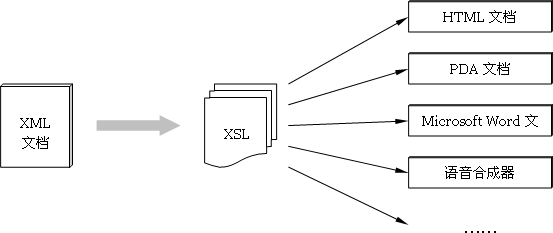
\includegraphics[scale=0.5]{xml_xsl.png}
\caption{可扩展样式表语言(Extensible Stylesheet Language,XSL)}
\label{xml_xsl}
\end{figure}

用XML规定的语言还有一个方便的特征,就是用这种语言的编写的文档可以轻松的自动生成。有些软件系统(通常具有底层数据库)可以用来生成大量易于在线传输和分析的数据,而生成的这些数据就能被转换成最适合每个用户浏览的格式。

有些组织为特定的主体开发了专用的XML,例如,化学家和化学工程师定义了化学标记语言(CML)以标准化分子数据的格式,CML包括大量有关化学的标记,给化学专业人员提供了共享和分析数据的通用格式。
	
XML是标记规约语言,XML文件则是数据。除非用户运行显示XML文件的程序(如浏览器),或者运行用它门进行操作的程序(如把数据转换成另一种格式的转换器或读取数据的数据库),或者运行修改它们的程序(如编辑器),否则什么都不会发生。


\section{XSLT}

XSLT(可扩展的样式表语言转换,Extensible Stylesheet Language Transformations),是用于转换 XML 的语言。

未来的网站将不得不向不同的浏览器并向其他web服务器以不同的格式传递数据。而 XSLT 则是一种将 XML 数据转换为不同格式的新的 W3C 标准。

XSLT 可以把 XML 文件转换为浏览器可识别的格式,比如 HTML,或者 WML - 一种用于许多手持设备的标记语言。

XSLT 还可以添加元素,并对元素进行删除、重新排列及排序,测试并确定显示哪些元素,等等。

	
XML和相关技术为信息管理和以各种方式在Web上有效地进行信息通信提供了强有力的机制。







\chapter{语义网}

“如果说 HTML 和 WEB 将整个在线文档变成了一本巨大的书,那么 RDF, schema, 和 inference languages 将会使世界上所有的数据变成一个巨大的数据库。” 

\begin{flushright}
——Tim Berners-Lee, Weaving the Web, 1999
\end{flushright}

$$\text{语义网(Semantic Web)}=\text{有意义的网络}$$

其中semantic(语义的)这个词指有意思的或与之相关的,语义网就是一种使用可以被计算机理解的方式描述事物的网络。

下面这样的句子可以被人类理解,但是怎样才能够被计算机理解呢?

\begin{compactitem}
\item 甲壳虫乐队是来自利物浦的著名乐队。
\item 约翰.列农是甲壳虫乐队的成员之一。
\item 唱片 "Hey Jude" 是由甲壳虫乐队录制的。
\end{compactitem}


陈述是由语法规则构建的,一门语言的语法定义了构建该语言的陈述所需的规则,这就是语义网的本质所在——以计算机应用程序可以理解的方式描述事物。



语义网和网页之间的链接没有关系,语义网描述的是事物之间的关系(比方说 A 是 B 的一部分,而 Y 是 Z 的成员)以及事物的属性(例如尺寸、重量、使用期限和价格等等)。

\section{语义网技术}

语义网不是快速发展的技术,RDF(资源描述框架,Resource Description Framework)是一种用于描述网络上的信息和资源的的标记语言,语义网使用 RDF 来描述网络资源。

RDF 是由那些拥有逻辑学和人工智能方面的学院背景的人们发展起来的。对于一般的开发人员的来说,它并不是特别容易被理解,其中,RSS就是一种用于构建语义网应用的快速发展的语言。

将信息置于RDF文件之中,这样的话,这些信息就有可能被计算机程序("web spiders")从网络中搜索、发现、收集、筛选、分析和处理。


举例来说,假如有关音乐、汽车、入场券(或者任何别的东西)的信息被存储于 RDF 文件,智能网络应用程序就会将信息从不同的源中进行收集,并将其整合,然后以一个有意义的方式将信息提交给用户们。


类似如下内容的信息:

\begin{compactitem}
\item 不同经销商的汽车价格
\item 药品信息
\item 航班时刻表
\item 工业备件
\item 书籍信息(价格、页数、编辑、年份)
\item 某人是谁
\item 事件的日期
\item 软件更新
\end{compactitem}


语义网不是可供搜索的免费文本,如果希望搜索或访问语义网,我们需要软件的协助。

要使用语义网,我们就需要 “语义网代理”(Semantic Web Agents)或 “语义网络服务”(Semantic Web Services),这些“代理”或“服务”会帮助我们在语义网上找到正在寻找的东西。

在语义网上,我们可能会搜索这些信息:

\begin{compactitem}
\item 最便宜的机票
\item 适合我的汽车的装饰
\item 书籍、电影或音乐
\item 天气预报
\item 时间表和日程
\item 股票价格和汇率
\end{compactitem}

在未来,要想在 Web 上找到任何信息,也许使用“语义网代理”就可以了。


\section{语义网安全}

用户的疑问是:“我能信赖语义网上的一个卖家吗?我能信任语义网上的一个买家吗?”。要解决上述问题,就需要访问更多 RDF 文件:

\begin{compactitem}
\item 信用卡信息
\item 银行信息
\item 语义网记录
\item 社会安全信息
\end{compactitem}


\begin{longtable}{|p{90pt}|p{90pt}|p{90pt}|p{90pt}|}
%head
\multicolumn{4}{r}{}
\tabularnewline\hline
Source	&Person ID	&Person Name	&Status
\endhead
%endhead

%firsthead
\hline
Source	&Person ID	&Person Name	&Status
\endfirsthead
%endhead

%foot
\multicolumn{4}{r}{}
\endfoot
%endfoot

%lastfoot
\endlastfoot
%endlastfoot
\hline
Citybank			&11223344	&Jim Green	&trustworthy\\
\hline
VISA				&11223344	&Jim Green	&trustworthy\\
\hline
Recorded			&11223344	&Jim Green	&unknown\\
\hline
US Social Security	&11223344	&Jim Green	&born 10-10-1984\\
\hline

\end{longtable}

通过使用类似的这些 RDF 文件,“语义网”代理就能够确定能够我们是否能信任正在打交道的这个人(能够通过 eBay 和 Amazon 之类的因特网交易公司来提供记录信息)。

\section{语义网支付}



要运营语义网,就必须开发支付手段,而易用的因特网“储蓄存款”可能成为此问题的解决方案。

“储蓄存款帐户”是一种只能接受存款的帐户。它可以为因特网上的所有提供便利,只要得到用户的 ID(或者电子邮件地址,很类似 PayPal),任何人都可以把钱存入指定的帐户。

通过使用这种支付手段,每个人都可以在因特网上公布他们的银行帐户,并在不需要中间人的情况下出售他们的汽车,这可能是未来的因特网银行的样子。

以后,用户需要卖一本书的情景可能如下:

\begin{compactitem}
\item 打开 OWL 代理
\item 在种类中输入 “Book”
\item 在新窗口中填写关于书的信息
\item 填写印在书上的 ISBN 号码
\item 选择“二手”,以及 "condition as new",并单击返回
\item OWL 代理会自动填写其余的部分
\item 作者、年份、页数... 现在所有的信息都完整了
\item OWL 代理已经搜集好您需要出售的书籍的所有信息
\end{compactitem}

最后,用户点击拍卖按钮。而对于“拍卖代理”,执行的动作可能是:

\begin{compactitem}
\item 拍卖代理打开了。
\item 用户填好了最低价格,然后点击“提交”。
\end{compactitem}

这样,用户的书籍就可以在因特网上进行拍卖了。


\section{语义网应用实例}


假设某个语义网系统用于通过因特网管理二手车的销售和购买,该系统可能包括两个主要的应用程序,其中一个针对希望购买汽车的人群,另一个针对希望出售汽车的人群。这里把这两个应用程序称为 IBA (I Buy Application) 和 ISA (I Sell Application)。

希望购买汽车的人群使用的 IBA 应用程序类似这样:

\begin{figure}[!h]
\centering
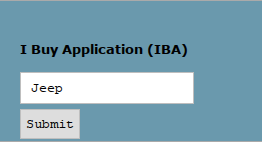
\includegraphics[scale=0.5]{semantic_web_example_buy.png}
\caption{IBA}
\label{semantic_web_example_buy}
\end{figure}


在真实世界的应用程序中,买方可能在第一次使用该程序时被要求标示自己的身份,然后买方的 ID 将存储在一个 RDF 文件中,ID 会把买方标示为一个带有名字、地址、电子邮件以及 ID 号的人。

当买方提交查询后,应用程序会返回一个待售汽车的列表,这个列表会按照年份、价格、位置和可用性进行排序。通过Web对 RDF 文件的搜索,此信息会不断地从 web spider 返回。

希望出售汽车的人群使用的 ISA 应用程序类似这样:

\begin{figure}[!h]
\centering
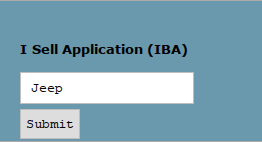
\includegraphics[scale=0.5]{semantic_web_example_sell.png}
\caption{ISA}
\label{semantic_web_example_sell}
\end{figure}


当卖方提交表单时,应用程序会向卖方请求更多的信息(包括年份、价格、位置等),并把卖方的 ID 和信息存储在一个 RDF 文件中,以供Web使用。

RDF 文件包含的信息类似:

\begin{compactitem}
\item ID:姓名、地址、电子邮件、ID 号等
\item 需求条目:名称、型号、价格等
\item 出售条目:类型、型号、图片、价格、描述等
\end{compactitem}

在幕后,这个 "ISA" 应用程序会创建一个带有许多 RDF 指针的 RDF 文件,RDF 指针是一种指向有关某事物的信息的指针(实际上是 URL),类似知识数据库。

比如,它会创建一个指向带有关于 person 信息的文件的指针,一个指向带有关于 Volvo 和 Volvo 型号信息的文件的指针,一个指向带有关于 Volvo 经销商和出售者信息的文件的指针,等等。


有关于此的优点在于用户不必对自己本人或汽车的型号进行描述,而这个 RDF 应用程序会为用户对信息进行整理。


RDF 是关于数据的数据 - 即元数据,RDF 文件经常会描述其它的 RDF 文件。将来有可能把所有的 RDF 文件连接起来构建一个语义网吗?没有人知道,但是总有人去尝试。


我们不认为语义网会依靠自己发展起来。它需要第三方的协助才能成为现实。不太可能的是,用户仅仅在因特网上发布 RDF 文件,就能够出售自己的汽车。

必须通过很多力量的参与,才能够发展类似上面的 "ISA" 和 "IBA" 应用程序。一方为所有的项目构建搜索引擎数据库,另一方则为其开发标准。可能是 eBay,或 Microsoft,或 Google,也可能是别的公司,但是总会有人去做。


或许有一天,用户将能够使用标准化的 RDF 文件在 Web 上收集有关几乎所有事物的信息。它可能免费,但也可能不得不为信息来付费,但在因特网上发布信息将比过去更加容易。





\bibliographystyle{plainnat}
\bibliography{csnotes}
\clearpage










\part{Computing Limitation}

字典对“限制”有很多解释,其中有“界限”和“令人恼怒的或无法忍受的事物”等意思,通过分析可以了解到,计算机硬件、计算机软件和我们要使用计算机解决的问题都对计算机的问题求解有限制,计算机科学发展到现在都无法回避的问题就是——计算的限制。

就像路障会阻断交通一样,这些硬件、软件和问题带来的限制也阻止了计算机中某些类型的处理。

\chapter{硬件的限制}

硬件带给计算的限制来自于几个因素。其一,数字本身是无限的,而计算机能表示的数字却是有限的,这种限制会导致算术运算错误,生成不正确的结果。其二,硬件就是硬件,也就是说,它是由易坏的机械部件和电子部件构成的,硬件部件会磨损。其三,在把数据从一个内部设备传递给另一个内部设备,或者从一台计算机传递到另一台计算机时会发生问题,造成信息损失。计算机科学的发展过程中分析了这每一种问题并提出了一些最小化它们的影响的策略。

\section{算术运算的限制}

计算机的硬件对整数和实数的表示法都有限制。

\subsection{整数}

在Pep/7中,运行算术运算的寄存器是16位的,如果只表示正数,它能存储的最大值是65535,如果既要表示正数,又要表示负数,它能存储的最大值是32767。

Pep/7是一台虚拟计算机,在真实的计算机中,如果计算机的字长是32位,那么它能表示的整数范围是$-2147483648$到$2147483647$。

有些硬件系统支持长字算术,从而将计算机的字长扩展到64位,这样计算系统可以表示的整数范围扩展到了$-9~223~372~036~854~775~808$到$9~223~372~036~854~775~807$,即使是这样的长度也不足以进行所有运算。

Henry~Walker在《The~limits~of~Computing》中引述了在棋盘中的每一个格子中按如下规则放置稻谷的例子:

\begin{compactitem}
\item 棋盘的第一格放1粒稻谷;
\item 棋盘的第二格放2粒稻谷;
\item 棋盘的第三格放4粒稻谷;
\item 棋盘的第四格放8粒稻谷;
\item 每个后继方格中的稻谷数量是前一格的两倍,直到64个棋盘格放完为止。
\end{compactitem}

这样就会发现第一行有$255(1+2+4+8+16+32+64+128)$粒稻谷,第二行有$65280$粒稻谷,第三行有$963040$粒稻谷,而后续进行下来,只是第$64$个格子就有$263$粒稻谷,约为$8\times 1018$粒,相当于$110000$亿蒲式耳。

通过这个例子可以知道,整数可以增长得非常快,增长得非常大。如果计算机字长为64位,只表示正数,那么最多只能表示第64个棋盘格中的稻谷数。如果想把64个棋盘格中的稻谷数加起来,计算机就做不到了,这样将会发生溢出。

一台计算机的硬件决定了它能表示的数字(整数和实数)的限制,不过用软件方法可以克服这种限制。例如,可以用一系列较小的数表示很大的数,下图展示了如果通过在每个字中放一位数字表示整数。

\begin{figure}[htbp]
\centering
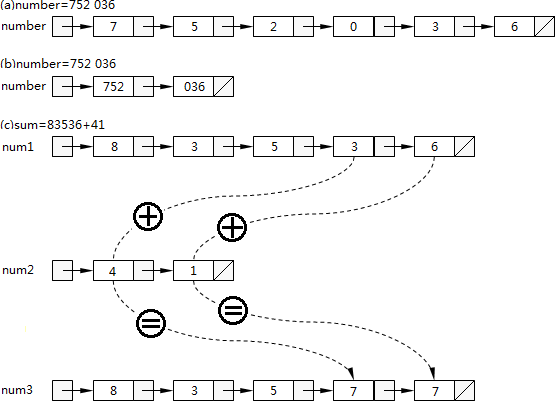
\includegraphics[height=220pt,keepaspectratio]{decimal.png}
\end{figure}

这样就可以实现用软件来表示非常大的数,操作这种形式的的整数的程序必须从最右边开始把每个数对相加,并且把进位加到左边一位的加法中。

\subsection{实数}

实数被存储为整数加说明小数点位置的信息。为了更好的理解为什么实数会带来问题,下面先看一个表示数字和小数点信息的编码模式。

为了便于讨论,我们假设计算机的内存单元大小相同,每个内存单元由一个符号和5个数字位组成。每当定义了一个变量或常量,赋予它的内存单元都由5个数字和一个符号构成。如果定义的是整数变量或整数常量,那么这个数会被直接存储起来。如果声明的是一个实数变量或实数常量,那么这个数将被存储为整数部分加小数部分,要表示这两部分,必须对该实数编码。

先了解编码后的数字是什么样的以及这些编码如何表示程序中的算术值,从整数开始。用5位数字能够表示的整数范围是-99999到+99999:

\begin{figure}[htbp]
\centering
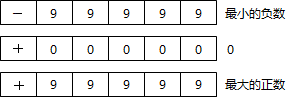
\includegraphics[height=60pt,keepaspectratio]{real.png}
\end{figure}

精度(precision,最多可以表示的有效位数)是5个数位。这个范围内的每个数都能被精确表示出来。如果用其中一个数位(如最左边的一位)表示指数则是下面的情况,例如:

\begin{figure}[htbp]
\centering
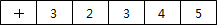
\includegraphics[height=15pt,keepaspectratio]{precision.png}
\end{figure}
表示的数字是$+2~345\times 10^3$,此时这5个数位表示的范围就大得多了,扩展到:
\[-9~999\times 10^9\mbox{到}+9~999×10^9\]
或
\[-9~999~000~000~000\mbox{到}+9~999~000~000~000\]
现在精度只有4位数字,也就是说,只能表示每个数中的4位有效位(signification digits,有效位指的是从左边的第一个非零数位开始,到右边的最后一个非零数位(或纯粹的零)结束的数字)。这意味着这个系统只能精确地表示4位数。对于更大的数会出现什么情况呢?

最左边的4位数字是正确的,其余的数字都被假设为0。右边的数位或者说最低有效数位将丢失。下面的例子说明了这种情况:

\begin{figure}[htbp]
\centering
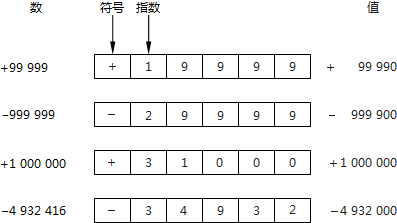
\includegraphics[height=120pt,keepaspectratio]{signification_digits.png}
\end{figure}

注意,我们只能精确地表示1000000,但不能精确地表示$-$4932416。我们的编码模式仅限于4位有效位,不能表示的数字被假设为0。

要扩展这种编码模式来表示实数,还要能够表示负指数,例如:
\[ 4394\times 10^{-2}=43.94\]
或
\[22×10^{-4}=0.0022\]
由于在我们的模式中,指数没有符号,所以必须对它稍加修改,把已经有的符号作为指数的符号,再在这个符号的左边加一个符号,作为数本身的符号。

\begin{figure}[htbp]
\centering
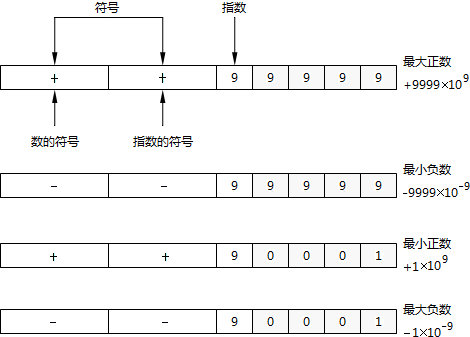
\includegraphics[height=200pt,keepaspectratio]{sign_number.png}
\end{figure}
现在可以表示$-9999×10^{-9}$到$9999×10^9$之间的所有数(精确到四位)了,包括所有的小数值。

假设想用这种编码模式求三个数$x$、$y$和$z$的和,可以先求$x$与$y$的和,再把$z$加到之前求得的结果上。也可以先求$y$与$z$的和,再把$x$加到之前求得的结果上。算术运算的结合律可以证明这两种方法得到的答案一样,但是真实的结果却未必。

计算机限制了实数的精度(有效位的位数)。下面用4位有效位加一位指数的编码模式求下列三个值的和:
\[ x=-1324\times 10^3~~y=1325\times 10^3~~z=5424\times 10^0\]
把$z$加到$x$和$y$的和上的结果如下:

\begin{table}[htbp]
\centering
\begin{tabular}{rrl}
$(x)$		& $-1324\times 10^3$ & 					\\
$(y)$		& $1325\times 10^3$	& 					\\
\hline
			& $1\times 10^3$		& $=1000\times 10^0$	\\
$(x+y)$	& $1000\times 10^0$	& 					\\
$(z)$		& $5424\times 10^0$	&					\\
\hline
			& $6424\times 10^0$	& $=(x+y)+z$	\\
\end{tabular}
\end{table}

把x加到y和z的和上的结果如下:

\begin{table}[htbp]
\centering
\begin{tabular}{rrl}
$(y)$		& $132500\times 10^0$	& 								\\
$(y)$		& $5424\times 10^0$		& 								\\
\hline
			& $1330424\times 10^0$	& $=1330\times 10^3$(截取4位有效数字)	\\
$(x+y)$	& $1330\times 10^3$	& 					\\
$(x)$		& $-1324\times 10^3$	&					\\
\hline
			& $6\times 10^3$	& $=6000\times 10^0=x+(y+z)$	\\
\end{tabular}
\end{table}

这两个答案的千位上的结果相同,但百位、十位和个位上的结果却不同,这叫做表示误差或舍入误差(representational(round-off)error),用来指代由于算术运算结果的精度大于机器的精度造成的算术误差。

$y$和$z$的和是精度为7位的数,但是只有4位被保存了下来。除了表示误差,浮点算术还有两个要注意的问题——下溢(underflow)和溢出(overflow)。当计算出的绝对值太小以至于给定的计算机不能表示时,将发生下溢。采用十进制数表示法,可以演示一个涉及到非常小的数的运算:

\begin{table}[htbp]
\centering
\begin{tabular}{rll}
$4210$			& $\times 10^{-8}$		& \\
$\times 2000$	& $\times 10^{-8}$		& \\
\hline
$8420000$		& $\times 10^{-16}$	& $=8420\times 10^{-13}$	\\
\end{tabular}
\end{table}

这个例子中的编码模式的最小指数是$-9$,而这时的指数$-13$太小了,所以不能表示这个数,因此这个运算的结果将被设为0。所有因为太小而不能表示的数都将被设为0。在这种情况下,这样做是合理的。

当计算出的绝对值太大以至于给定的计算机不能表示时,将发生溢出(overflow)。溢出是更加严重的问题。因为一旦发生溢出,没有合理的解决办法。例如,下列运算的结果:


\begin{table}[htbp]
\centering
\begin{tabular}{rll}
$9999$			& $\times 10^{9}$		& \\
$\times 1000$	& $\times 10^{9}$		& \\
\hline
$9999000$		& $\times 10^{18}$		& $=9999\times 10^{21}$	\\
\end{tabular}
\end{table}

在当前例子中的编码模式中就不能存储。而处理办法要与下溢的处理保持一致,可以把结果设置为$9999\times 10^9$,即模式中的最大实数值。而我们仅凭直觉也会发现这是不对的。另一种方法是停止运算报错。

浮点数可能发生的另一种错误是化零误差(cancellation error),由于计算机精度限制,当相加或相减的两个数的量级相差太大时会出现这种误差。下面是一个例子:
\[(1+0.00001234-1)= 0.00001234\]
算术运算的法则可以证明这个等式是正确的。但如果用计算机来执行这个运算却可能会出现下面的情况:

\begin{table}[htbp]
\centering
\begin{tabular}{rrl}
	& $100000000$	& $\times 10^{-8}$	\\
$+$& $1234$			& $\times 10^{-8}$	\\
\hline
	& $100001234$	& $\times 10^{-8}$	\\
\end{tabular}
\end{table}
因为只有4位精度,所以结果将变为$1000×10-3$。计算机再减去1:

\begin{table}[!h]
\centering
\begin{tabular}{rrl}
	& $1000$	&$\times 10^{-3}$	\\
$-$& $1000$	&$\times 10^{-3}$	\\
\hline
	& $0$			& 						\\
\end{tabular}
\end{table}

这是计算机的运算结果,是0而不是$0.00001234$。

在计算机的算术运算中,整数和实数,无论正数还是负数,都会发生溢出。另外要注意的是,第一,实数运算的结果通常与我们通常预期的不同。第二,如果处理的数非常大或非常小,要注意执行运算的顺序。

\section{部件的限制}

在计算机系统中,硬件故障的问题确实存在,硬盘可能会损坏,文件服务可能会崩溃,网络也可能会中断,于是J.A.N.Lee杜撰了Titanic效应这个词来形容系统崩溃的严重程度超出了设计者的想象力。硬件故障确实会发生,最后的解决方法是进行防御性维护。在计算领域,这意味着定期检测硬件的问题,替换损坏的零件。

防御性维护还要保证放置计算机的物理环境适宜,大型计算机常常需要具有空调和无尘的房间。PC也要求保持相应的运行环境。计算机科学中使用术语“bug”来表示计算机错误。后来,Edsger~Dijkstra反对使用这种术语,他认为这种叫法会使人们产生错觉以为计算机的错误超出了程序员的控制。他认为bug是一种智力欺骗,隐藏了程序自己制造错误的事实。

关于计算机部件限制的所有讨论都有一个前提,就是计算机硬件在设计和制造阶段都经过了全面的测试。

\chapter{通信的限制}

计算机之内和计算机之间的数据流是计算的生命血液。因此,一定要保证数据不被破坏。实现这一点的策略叫做检错码和误差校正码。检错码可以判断出在数据传输过程中是否发生了错误,并警告系统。误差校正码不仅能检测出发生的错误,还能判断出正确的值是什么。

\section{校验位}

校验位用于检测存储和读取或发送或接收一个字节的过程中发生的错误。校验位是在使用这种模式的硬件中的每个字节上加上了一个位。这个位用于确保9位数值(一个字节加一个校验位)中的1的个数是奇数(或偶数)。

奇数奇偶校验要求一个字节加一个校验位中有奇数个1。例如,如果一个字节中的值是11001100,那么校验位是1,这样才能得到奇数个1。如果字节中的值是11110001,那么校验位是0。

当从内存中读取或接收了一个字节时,将计算其中1的个数(包括校验位)。如果1的个数是偶数,说明发生了错误。如果硬件采用这种模式,每个字节将多一个附加位,只有硬件才能访问这个位,用于检测错误。偶数奇偶校验的模式与奇数奇偶校验的相同,只是其中必须有偶数个1。

\section{校验数位}

上述模式的一个软件变体是求一个字节中的每个数位的和,然后把和的个位与字节中的数存储在一起。例如,对于数字34376,每个数位的和是23,因此,存储的数就是34376$-$3。如果这个数中的4变成了3,就可以检测到错误。但是,如果7变成了6,而6变成了7,那么数位的和仍然是正确的,但是数却是错的。

这种模式可以扩展为多一个附加位,可以是奇数位的和的个位数。例如,34376可以存为34376$-$23,3是所有数位和的个位数,2是第1位、第3位和第5位的和的个位数。这种方法能捕捉到相邻数位之间的传输错误,但却会漏掉其他的传输错误。当然,还可以存储偶数位的和的个位数,也就是说,要检测的错误越重要,检测算法就越复杂。


\section{误差校正码}

如果对于一个字节或一个数保存了足够的信息,那么可以推导出错误的数位应该是什么。极端的冗余是对每个存储的值都保留两个独立的副本。如果发现奇偶校验或校验数位有错,那么可以查阅另一个副本以得到正确的值。当然,连个副本可能都有错。误差校正码主要用于硬盘驱动器或CD,CD表面的不完整性会破坏数据。

\chapter{软件的限制}

计算机软件(包括商业软件等)存在错误,这种问题并非由懒惰引起的,而是由软件的复杂度引起的。随着机器的功能越来越强大,计算机能够解决的问题也变得越来越复杂。以前一个问题由一个程序员解决,现在成了一个问题由一组程序员解决,最后一个问题由一组程序员组解决。

\section{软件的复杂度}

大型软件项目的大小和复杂度几乎一定会导致产生错误。虽然软件测试能够证明存在bug,但是不能证明不存在bug。我们可以测试软件,发现问题,修正问题,然后再测试软件。随着我们不断发现问题,解决问题,我们对软件的信心也会逐渐增强。但我们永远不能确保已经除去了所有的bug。软件中潜藏着其他的bug,我们还没有发现,这种可能性将一直存在。

Nancy~Leveson在《Communications~of~the~ACM》中指出过,20世纪60年代出现的计算分支软件工程的目标就是把工程原则引入软件开发。目前软件工程已经涉及到对抽象的角色的更深理解、模块性的引入以及软件生命周期的概念等。

虽然大多数概念来自工程学,但它们必须适合处理更抽象的数据时会发生的特殊问题。硬件设计受实现设计所用的材料的指导和限制,软件则主要受人类能力的限制,而不是物理限制。Leveson博士指出,“因此,前50年的特征是学习这个领域的限制,这与人类能够处理的复杂度的限制息息相关。”

构建软件的重点已经改变了。以前是构建新软件,而今天,现有软件的维护和升级的问题越来越多,逐渐占据了中央舞台。

随着计算机软件系统变得越来越大而且需要整组的程序设计人员,我们开始分析人类协作的方式,以便设计出能辅助人们有效协作的方法。

\subsection{当前提高软件质量的方法}

虽然不可能使大型软件系统完全没有错误,但是并不意味着我们应该放弃,我们可以采用某些策略来提高软件的质量。构建好的软件的最佳方法是从项目一开始就关注它的质量,应用软件工程的规则。


\subsection{软件工程}

以前在计算机问题求解的过程中,要经历三个阶段,即开发算法、实现算法和维护程序。而从定义明确的小任务转移到大型的软件项目,那么还需要增加两个阶段,即制定软件需求和规约。

软件需求(software~requirement)是用概括而精确的语句列出软件产品提供的功能。软件规约(software~specification)则详细说明了软件产品的功能、输入、处理、输出和特性,软件规约提供了设计和实现软件所必需的信息。软件规约说明了程序能够做什么,而不是怎么做。

Leveson博士把软件生命周期看作软件工程要规划的一部分。所谓软件生命周期指的不仅是编码,而是软件的开发和升级。因此,软件的生命周期包括下列阶段:
\begin{compactitem}
\item 需求分析;
\item 制定规约;
\item 设计(高层和低层);
\item 实现;
\item 维护。
\end{compactitem}

所有阶段都要执行验证操作。需求是否精确反映了需要的功能?规约是否精确反映了满足需求所需的功能?高层设计是否精确反映了规约中的功能?设计中的每个后继层是否精确实现了上一层的功能?代码实现是否与设计相符?维护阶段实现的改变是否精确反映了想要的改变?这些改变的实现是否正确?

在使用计算机解决实际问题时,随着问题的增大,验证操作也会变得越来越重要,越来越复杂。虽然设计和代码的测试是整个过程很重要的一部分,但也只是一小部分。在一个典型的项目中,有一半错误是在设计阶段发生的,而实现阶段发生的只是一半错误而已。这个数据会引起一些误解,如果以修正错误的代价为衡量标准,那么在设计过程中越早发现错误,修正错误的花费越小。

大型软件产品是由程序员组开发的,程序设计小组使用的两种有效验证方法是走查和审查。这些是正式的小组活动,目的是把揭露错误的责任从个人转移到小组。由于测试非常耗时,而且错误发现的越晚,代价越高,所以这种活动的目标是在测试开始前发现错误。

使用{\heiti 走查(walk-through)}的方法,将由一个小组用样本测试输入手动模拟设计或程序,在纸上或黑板上跟踪程序的数据。与全面的程序测试不同,走查并非要模拟所有可能的测试情况,它的目的只是模拟程序员选择的设计或实现程序需求的方法。

在{\heiti 审查(inspection)}过程中,将由一位读者(绝对不是程序的作者)逐行读出程序的需求、设计或代码。审查员会预先得到相关资料,而且预期会仔细阅读过这些资料。在审查过程中,审查员会根据审查报告中的记录指出错误之处。他们在预审时已经注释了许多错误。大声朗读的过程只是为了发现更多的错误。与走查一样,小组讨论的主要好处在于讨论是在所有小组成员之间进行的。程序员、测试员与其他小组成员的沟通会在测试开始前发现更多的程序错误。

因此,走查是由一个小组手动地模拟程序或设计的验证方法,而审查是由团队成员之一逐行读出设计,由其他成员负责指出错误的验证方法。

在高层设计阶段,要拿设计与程序需求进行比较,以确保设计方案包括了所有必需的功能,以及该程序或模块能够与系统中的其他软件正确地连接起来。在低层设计阶段,设计已经具有很多细节,在实现它之前,一定要进行预审。完成编码后,要再审查一次编译过的清单。审查(或走查)可以确保实现与需求和设计一致。成功地完成审查意味着可以开始程序测试了。

走查和审查都要以一种无威胁的方式执行。这些小组活动的重点是去除产品中的瑕疵,而不是设计或代码的作者采用的技术方法。由于这些活动的主持人都不是作者,所以针对的是错误,而不是人。

在过去的10年或15年中,Carnegie Mellon大学的软件工程学院在规范大型软件项目的审查过程的研究方面扮演了重要的角色。

SEI~Software~Engineering~Process~Group(SEPG)Conference上的1篇论文报告了一个项目,该项目采用小组走查和正式审查结合的方式能够把产品的错误减少86.6\%,这一过程要应用于生命周期的每个阶段。下表展示了在一个维护项目的生命周期的各个阶段发现的每1000行源代码(KSLOC)中的错误数。
\begin{table}[!h]
\centering
\caption{维护时发现的错误}
\begin{tabular}{|l|l|}
\hline
阶段					& KSLOC中的错误数				\\
\hline
系统设计				& 2								\\
\hline
软件需求				& 8								\\
\hline
设计					& 12								\\
\hline
代码审查				& 34								\\
\hline
测试活动				& 3								\\
\hline
\end{tabular}
\end{table}

在维护阶段,50多万行的程序被附加了40000行源代码。除了测试活动外,每个阶段都要进行正式的审查。

在软件工程中,对软件的规模进行了量化。Space~Shuttle~Ground~Processing~System具有50多万行代码;Windows 95具有1000万行代码。大多数大型项目的代码数介于这两者之间。

由于大型项目的复杂度,所以要编写没有错误的代码是不可能的。下面是预计错误量的一个参考标准:
\begin{compactitem}
\item 标准软件:每1000行代码25个bug;
\item 好的软件:每1000行代码2个错误;
\item Space~Shuttle软件:每10000行代码少于1个错误。
\end{compactitem}

E.N.Adams在《IBM~Journal~of~Research~and~Development》中估计到,在尝试删除大程序中的错误时,约有15\%$\sim$50\%的操作会引入新的错误。

在分析软件故障的过程中会发现,虽然可能的错误只有一种——编码错误,但是更深入追究下去,会发现严重的设计失误。几乎所有软件在特定条件下都会有意想不到的行为。这里的低级错误是由于缺乏软件工程的经验而构建了依靠软件进行安全操作的机器。此外,软件整体的不安全设计比某个编码错误重要得多。

\subsection{正式验证}

在计算机科学中,人们设想是否可以用工具来定位设计和代码中的错误,甚至可以不必运行程序就能进行验证。这种设想来自于几何学的比喻,我们不必对每个三角形都证明一次勾股定理,这说明该定理适用于我们用过的每个三角形。我们可以用数学方法证明几何定理,那么用类似的方法证明计算机程序同样可行。

程序正确性的验证独立于数据测试,是计算机科学理论研究的一个重要领域。这项研究的目标是建立证明程序的方法,就像证明几何定理的方法一样。现在已经有证明代码满足规约的必要方法,但是证明通常比程序本身更复杂。因此,验证研究的重点是尝试构建自动化的程序证明器,即验证其他程序的检验程序。

已经有正式的方法可以成功地验证计算机芯片的正确性。一个著名的例子是验证执行实数算术运算的芯片,这项验证获得了英国女王技术成就奖(Queen's~Award~for~Technological~Achievement)。牛津大学的程序设计研究组的组长C.A.R.Hoare与MOS~Ltd.一起对芯片是否满足规约进行了正式验证。同时执行的还有一种传统的测试方法。《Computing~Research~News》报道如下:
\begin{verbatim}
“正式的开发方法在两组之间的竞赛中取得了胜利,它只用了大约12个月的时间
就完成了,与预计的时间要短。此外,正式的设计指出了许多非正式设计经过几
个月的测试而没能指出的错误。最后的设计不仅质量更高,花费更小,完成得也
更快。”
\end{verbatim}
硬件层的正式验证技术的成功有望带来软件层验证的成功,但是,软件比硬件复杂得多,所以在不久的将来,不会出现太大的突破。

\subsection{开源运动}

在计算早期,软件(包括它的源代码)是与计算机绑定在一起的。从20世纪70年代开始,公司开始保留源代码,软件从而成为了一项大生意。

随着Internet的出现,世界各地的程序员可以轻易得到一个软件产品的简单的版本,而且程序员仍然对扩展或改进程序充满兴趣。跟踪项目进展的“善意独裁者”掌控者大部分开源项目。如果一种改变或改进获得了同辈开发人员的认可,加入了新的软件版本,那么它一定更出色。

Linux是最著名的开源项目,Linus~Torvolds以UNIX为蓝图,开发了这种操作系统的第一个简单版本,并且一直在观察着它的发展。Linux更像一个即将出现的模式的教科书示例。开源运动是一个大规模的奇迹,SourceForge是一个开发者的Web站点,现在已经具有18000多个开源项目,145000个程序员在为此忙碌着。


\section{臭名昭著的软件错误}

计算领域中的每个人都有自己喜欢的软件恐怖故事。这里只列出一些小例子。

1990年1月,AT\&T的长途电话网络由于电子交换系统的软件错误中断了9个小时。那天AT\&T收到了1.48亿个长途电话和800电话,只有50\%被转接了出去。这次故障还引起了数不清的间接破坏:
\begin{compactitem}
\item 宾馆丢失了预订电话。
\item 汽车出租代理丢失了租车电话。
\item 美国在线的预订系统通信量降低了2/3。
\item 电话推销商估计损失75000美元。
\item MasterCard不能处理200000个信贷批准。
\item AT\&T损失了6000万到7500万美元。
\end{compactitem}

正如AT\&T的主席Robert~Allen所说的,“这是我从商32年来最可怕的噩梦。”

怎么会出现这种情况呢?交换软件的早期版本是能够正确运行的。升级后的系统代码中的软件错误使它对故障交换响应得更快。这个错误发生在一个C代码的break语句中。像Henry~Walker在《The~Limits~of~Computing》中指出的,这次崩溃说明了许多软件故障的共同点。

在该软件发布之前,它已经经过大量的测试,而且已经正确运行了一个月。除了测试外,研发过程中还进行过代码检阅。一位程序员犯了这个错误,但是其他检阅代码的程序员却没注意到这个错误。一个相对罕见的事件序列触发了这次故障,这是事先很难预料得到的。而这个错误出现在为改进一个正确运行的系统而设计的代码中,即出现在维护阶段。

一位美国空军的监察员发现,美国核导弹舰队的关键部分和部件的计算机跟踪中出现了令人费解的错误。这些错误包括重复的、遗漏的和不正确的序列码,遗漏的和不正确的零件编号,以及不正确的设备数量和位置。10个发组井在要发射导弹时电量不足。监察员认为这些问题源自于系统缺乏输入和检测盘点数据的训练。这是GIGO(garbage~in, garbage~out,无用输入无用输出)的一个好例子。

另外,即使软件系统操作正确,如果使用的数据不好,答案也会错误。使用的数据好坏决定了答案的好坏。这种情况就是GIGO,即无用输入,无用输出。在心情一样地情况下,让人困惑的系统使用起来也更容易出错。

流传最广的软件事故与一台计算机化的放射治疗仪Therac-25有关,在1985年6月到1987年1月之间,Therac-25造成了6次重大的用药过量事故,导致了病人死亡或严重受伤。这些事故据说是应用医疗加速器35年以来最严重的放射事故。

深入分析软件故障时会发现,虽然可能的错误只有一种——编码错误,但是深入追究下去,会发现严重的设计失误。Leveson和Turner在《KIEEE~Computer》发表的文章中加入了下面的评论:
\begin{verbatim}
“从Therac-25的故事可以得到的教训是仅仅关注个别的软件bug不能保证系统安全。
几乎所有软件在特定条件下都会有意想不到的行为。这里的低级错误是由于缺乏
软件工程的经验而构建了依靠软件进行安全操作的机器。此外,软件整体的不安全
设计比某个编码错误重要得多。”
\end{verbatim}

1991年2月25日,海湾战争期间,一枚飞毛腿导弹击中了美国陆军的军营,有28名士兵死亡,100多人受伤。由于软件错误,位于沙特阿拉伯Dhahran的美国爱国者导弹发射器没能成功跟踪并阻截伊拉克的飞毛腿导弹。不过这个错误不是编码错误,而是设计错误。其中的一个运算涉及到1/10的乘法,这个数在二进制中是无尽的。在100个小时的发射操作中,这种算术错误累积的误差是0.34秒,足够使导弹偏离它的目标。

审计院总结道:
\begin{verbatim}
“爱国者从来没有阻击过飞毛腿导弹,而且我们也没有预计它要连续运行这么长时间。
事故发生两周前,陆军官方收到的以色列数据说明在系统连续运行了8小时后,已经
出现了误差。于是陆军官方修改了软件,以提高系统的精确性。但是直到2月26日,
飞毛腿导弹事件发生后的第二天,修改好的软件才到达Dhahran。”
\end{verbatim}

Gemini~V的着陆地点距预计的点100英里。什么原因?是导航系统的设计没有将地球围绕太阳的转动考虑在内。

1999年10月,美国发射的火星气候轨道探测器(Mars~Climate~Orbiter)进入了火星大气层,进入点比预计的低100公里,导致飞船烧掉了。火星气候轨道探测器任务失败调查小组的主席Arthur~Stephenson总结道:
\begin{verbatim}
“导致太空船销毁的根本原因是一个地面导航软件没能像NASA宣布的那样把英语
转换成度量单位……失败调查小组还发现了其他导致错误的重要因素,它们使错误
拖延下来,结果使飞船进入火星的路径出现了很大的误差。”
\end{verbatim}

1962年7月美国发射的水手1号(Mariner~1)金星探测器几乎一发射就转变了航向,不得不被销毁了。这个问题是由下面这行Fortran代码引起的:
\begin{verbatim}
DO 5 K=1.3
\end{verbatim}
其中的句号应该是个逗号。由于这个输入错误,价值1850万美元的太空探索飞船就这么毁掉了。

软件错误并不只是美国政府才会犯。

1996年6月4日,欧洲空间局发射的无人火箭Ariane5在升空40秒后就爆炸了。这架火箭开发了十几年,开发费是70亿美元。火箭本身和它携带的货物价值5亿美元。究竟发生了什么问题呢?一个相对于平台的水平速率是64位的浮点数大于32767,结果被转换成了16位的整数,导致火箭转变了航迹,然后解体,爆炸。

\chapter{问题}

对有些问题,能够轻松地开发和实现计算机解决方案。对有些问题能实现计算机解决方案,但不能得到日常生活中的结果。有些问题在具有足够的计算机资源的情况下能够开发和实现计算机解决方案。有些额外的问题可以证明是没有解决方案的。

\section{算法分析}

在应用计算机求解问题时,有些问题能够轻松地开发和实现解决方案,有些问题能实现解决方案,但不能得到日常生活中的结果,还有些问题只有在具有足够的计算资源的情况下能够开发和实现解决方案,另外还有一些问题可以证明是没有解决方案的。

在解决实际问题时,大部分问题的解决方案不止一种,如果要询问去Joe’s Diner的路,可能会得到两种等价的正确答案:

1、“走高速公路,到Y’all~Come Inn之后,左转。”

2、“走winding~country~road,到Honeysuckle~Lodge之后,右转。”

虽然这两种答案不同,但无论走哪条路,都可以到达Joe’s~Diner,所以这两个答案都是正确的。

\begin{figure}[!h]
\centering
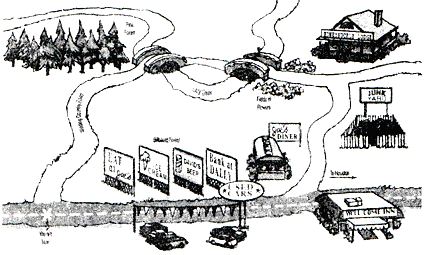
\includegraphics[height=140pt,keepaspectratio]{joe_diner.png}
\end{figure}

如果问路的请求中包括特殊要求,那么一种解决方案可能比另一种好。例如,“我要迟到了,哪条路到Joe’s Diner最快?”这时第一种方案更合适。如果要求是“有没有安静的小路可以到Joe’s Diner?”就要用第二种方案。如果没有特殊要求,那么可以根据个人喜好进行选择,不同的人面临不同的选择,最终选择的结果也不尽相同。

在评估某一问题的不同的解决方案时,一个比较标淮是效率。如果把效率当作一个非形式化的概念,会很容易认为一个程序比另一个效率更高。另一方面,也就没有机会具体考虑什么叫效率。

在实践中会发现有些程序运行得非常快,有些却很耗时。直觉告诉我们,执行得快的程序效率高,而执行慢的程序其效率相对较低。但这种直觉是有误导性的。

尽管运行时间和效率是相互关联的概念,它们并不完全相同,因为问题的内在难度是不同的。

用一个低效率的程序解决一个简单的问题所花的时间可能比用一个高效率的程序解决复杂问题所花的时间少得多。效率必须考虑到问题的难度。当谈到效率时,最好考虑到解决同一问题的不同算法的相对效率。

在计算机科学的高级课题中,衡量算法的相对效率是一个主要的课题,这个课题被称为算法分析(analysis of algorithm)。尽管理解算法分析需要用到数学知识而且要进行细致的思考,但我们还是可以通过比较几个简单算法的性能大概了解怎样进行算法分析。

\section{评估算法效率}

假设给出了解决同一问题的两个算法。要判断哪一种算法效率更高,应该怎样进行比较呢?

在某些情况下,可以利用经验进行衡量。如果想判断哪个算法能更快地解决特定问题,可以执行这两个程序,看每一个程序运行的时间。假设可以在现代计算机的计算速度下精确地测量时间,那么这种方法可以精确提供这个问题的每种解法的耗时信息。但是这种方法还是有误导的可能,尤其是当算法的运行时间取决于输入数据的时候。一个算法在输入一组数据时运行很快,也有可能在输入另一组数据时运行很慢。一些算法在有少量的输人数据时可能运行得很好,但当数据量增大时运行效果会降低很多。

在现实中,同一个问题可能有多个等价有效解决方案。在计算机科学中,关于算法的选择通常是由效率决定的。哪个算法花费的计算时间最少?哪个算法完成作业的工作量最小?这里我们指的是计算机所做的工作量。

当评估算法效率时,计算机科学家使用字母$N$表示问题规模,而不管它是怎样得出的。算法分析的核心问题是确定一个算法的运行时间是怎样随着N值变化的。当N值变大时,N和算法运行时间之间的关系被称为该算法的计算复杂性(computational~complexity)。


要比较两个算法的工作量,首先要定义一组客观的度量标准。算法分析是理论计算机科学的一个重要研究领域。下面介绍算法分析的一小部分,通过比较两个任务相同的算法,来理解算法的复杂度构成的一个从易于解决到不能解决的连续统。

程序员衡量两个不同算法执行的工作时,首先想到的是对算法编码,然后对比两个程序的运行时间。执行时间较短的算法显然是比较好的算法。但是,实际情况是,使用这种方法,只能确定程序A在特定的计算机上比程序B有效。执行时间是特定计算机特有的。当然,可以在所有可能的计算机上测试算法,但我们需要一个更通用的方法。

第二种方法是计算执行的指令输或语句数。但是,使用的程序设计语言不同,以及程序员的个人风格不同,都会对这种衡量方法有影响。为了标准化这种衡量方法,可以计算算法中执行关键的循环的次数。如果每次迭代的工作量相同,那么这种方法就给我们提供了算法效率的有效衡量标准。

另一种方法是把算法中的一个特定基础操作分离出来,计算这个操作执行的次数。例如,假设要求一个整数列表中的元素的和。要衡量所需的工作量,就要计算整数加法操作的次数。对于有100个元素的列表,需要99次加法运算。但要注意,并非真的要去计算加法运算的次数,它是列表中的元素个数($N$)的函数。因此,可以用$N$表示加法运算的次数,对于有$N$个元素的列表,需要$N-1$次加法运算。这样现在就可以比较一般情况的算法性能,而不必只是比较特定列表大小的情况了。

实际上,关于算法效率的大部分真知灼见是帮助我们理解一个算法的性能怎样随着问题规模的变化而改变。
对很多算法来说,问题规模是很容易量化的。例如,在经典算法(如测试素数或找最大公因子)中随着数字变大,运算速度会大大降低。在这类算法中,数字的大小提供了一个衡量问题规模的合适标准。对于操作数组的算法(如排序算法),可以把数组中的元素个数作为问题的规模。

\section{评估选择排序算法的效率}

选择排序算法有很多优点。首先,它的算法很容易理解;其次,它解决了排序这个问题。但是,还存在其他一些更有效的排序算法。而且,效率最高的排序算法需要很高的技巧。

通过评估算法的效率,可以进一步改进算法。尽管到目前为止我们还不能充分改善选择排序的效率,但现在正在考虑它的效率到底如何。

一个很有趣的问题就是确定用选择排序算法对某一输入数组进行排序需要多长时间,这里有两种方法可供参考:

(1)可以运行该程序看它需要多少时间。不过可以使用计算机内部的时钟得到结果。

由于程序在现代计算机中运行的速度非常快,通常运行的时间不到一秒,因此用秒表根本不可能测出运行的时间。

(2)可以更一般地考虑程序的操作,对它的行为进行量化。

\section{测试程序的运行时间}

为了确定运行一个程序需要的时间,常用的方法是用系统库来记录所需要的时间。ANSI接口time.h输出一个名为clock的过程,它能返回执行某一程序所用的以计算机处理单元为单位的时间量。clock函数返回的类型是与机器相关的时钟单位,但是可以通过以下的表达式将它转化成以秒来计算的时间形式:
\verb|(double) clock() / CLOCKS_PER_SEC|
如果把开始时间和结束时间分别存储于变量start和finish中,可以用下列代码计算执行一个操作所需的时间:
\begin{verbatim}
double start, finish, elapsed;
start = (double) clock() / CLOCKS_PER_SEC;
. . . 执行某些操作
finish = (double) clock() / CLOCKS_PER_SEC;
elapsed = finish – start;
\end{verbatim}

于是就可以用上述方法计算选择排序算法的运行时间。对大小不同的数组调用SortIntegerArray函数所需要的时间见下表。
\begin{table}[!h]
\centering
\caption{选择排序算法的运行时间(以毫秒为单位)}
\begin{tabular}{|l|l|l|l|}
\hline
N 			& 运行时间(毫秒)	& N 				& 运行时间(毫秒)			\\
\hline
10			& 0.13				& 100				& 9.67						\\
\hline
20			& 0.33				& 200				& 37.33						\\
\hline
30			& 1.00				& 400				& 146.67						\\
\hline
40			& 1.47				& 800				& 596.67						\\
\hline
50			& 2.40				& 					& 								\\
\hline
\end{tabular}
\end{table}


在这张表中,$N$表示数组中元素的个数,而“运行时间”列表示使用选择排序算法对相应的数组进行排序所需要的时间(时间单位为毫秒)。

这张表显示了一个有趣的现象。当$N$很小时,选择排序算法需要的时间很少,但随着$N$的增大,执行选择排序算法需要的时间显著增加。举个例子来说,如果数组包含30个值,SortIntegerArray排序这个数组需要1毫秒,当达到800个值时,需要的时间超过0.5秒。而商业应用通常需要对10~000、100~000甚至更多的数进行排序。对这种规模的数组,选择排序算法的速度将慢得惊人。

\section{选择排序的算法分析}

要理解实现某种算法的程序的运行时间的变化规律,首先要明白算法的工作原理。考虑选择排序的时间数据,当$N$为50时,执行算法需要2.4毫秒,而当$N$为100时,需要的执行时间为9.67毫秒,差不多是$N$为50时需要时间的4倍。

我们从表中其他部分也可以得到这样的结论:数组的元素个数增加一倍,那么所需要的时间是原来的4倍。我们把这个排序算法称为具有平方律(quadratic)的性质,即执行时间和输入数组大小的平方成正比。

选择排序算法具有平方律性质的事实其实并不奇怪,只要思考一下算法的执行过程就可以理解。在对一个具有8个元素的数组进行排序时,该算法需要执行8次外层for循环。第一个循环周期找出8个数中的最小值,下一个循环周期则在剩下的7个元素中找到最小值,依次类推。

程序执行的操作次数和该数组的个数成正比,对上面的例子,需要执行的操作的次数为:
\[8+7+6+5+4+3+2+1=36\]
更一般的情况,假如数组有N个数,选择排序需要的时间与下面的和成正比,即:
\[N+N-1+N-2+\cdots+3+2+1=\dfrac{N^2+N}{2}\]
于是,可以从上式的$N^2$中很容易看出这种平方律的性质。

各种排序算法的效率差别很大,对于具有较少元素的数组来说,使用选择排序算法这种简单的算法很合适,但对于具有较多元素的数组,该算法就不合适了。

应用数学方法预测算法效率的过程称为算法分析(analysis of algorithm),通过学习如何分析某一算法效率的问题,对于我们以后评价某一问题适合用哪种算法是非常有用的。



\chapter{大O分析}

计算机科学家用O(读作Big Oh)表示算法的计算复杂性。这个符号为大O标记,由一个大写的字母口及其后的一个用圆括号括起的公式组成,该公式表示运行时间随问题规模变化的函数。

在计算机科学中,当用操作输入的大小的函数来衡量工作量时,可以用数量级表示这个函数的近似值。字母O代表单词order(顺序),因为它用于短语on the order of,所以指的是近似值。

函数的数量级是以问题的大小为参数的函数中的最高项。因此,可以得到大O标记(Big-O Notation)的正式定义如下:
\begin{verbatim}
以函数中随着问题的大小增长得最快的项来表示计算时间(复杂度)的符号称为大O标记。
\end{verbatim}
从而使用大O分析可以根据由问题大小决定的增长速率来对比算法,从而说大O标记指出了一个程序的运行时间是怎样随着问题规模的变化而变化的,而降低一个算法的计算复杂性可以大大提高运行效率。

例如,如果
\[f(N)=N^4+100N^2+10N+50\]
那么$f(N)$的数量级是$N^4$,用大O符号表示就是$O(N^4)$。也就是说,对于较大的$N$,$N^4$在函数中占支配地位。$100N^2+10N+50$并非不重要,只是随着$N$越来越大,其他的因素就会变得无足轻重,因为$N^4$支配着这个函数的数量级。



对于大O符号(Big-O~Notation)的正式定义是,以函数中随着问题的大小增长得最快的项来表示计算时间(复杂度)的符号,从而使用大O分析可以根据由问题大小决定的增长速率来对比算法。至于为什么可以舍弃低数量级的项,可以考虑这样的例子,如果我们想要购买大象和金鱼,考虑两家宠物销售商,我们只需要对比大象的价格,金鱼的价格根本微不足道。

\begin{figure}[htbp]
\centering
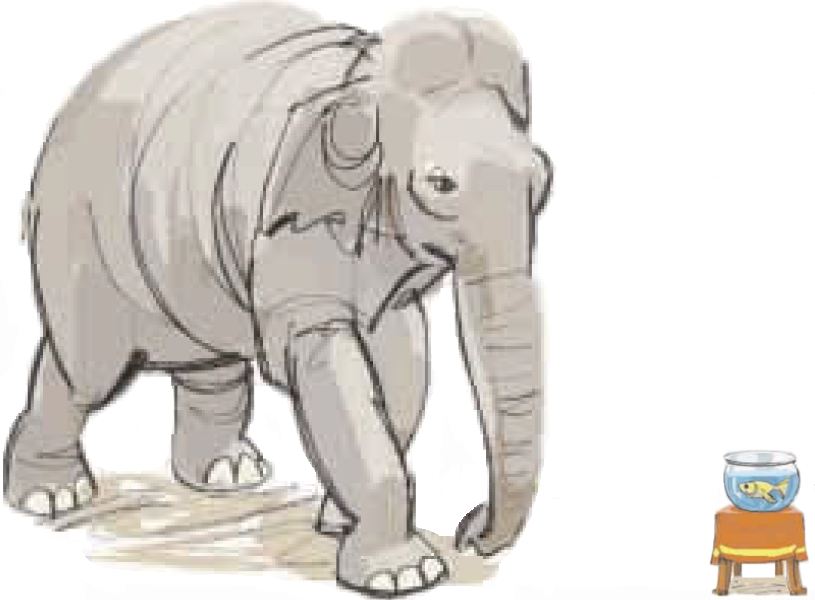
\includegraphics{elephant_goldfish.png}
\end{figure}

同样地,在算法分析中,随着问题大小增长得最快的项支配着整个函数,把其他项明显地降到了“噪音”的水平。大象太大以至于我们可以忽略金鱼。同样地,对于较大的$N$,$N^4$比$50$、$10N$,甚至$100N^2$都大得多,以至于可以忽略这些项。这并不意味着这些项对计算时间没有影响,只是说它们在$N$比较“大”时对我们的估计没有显著影响。


\section{什么是N}


$N$表示问题的大小。大多数问题都涉及到数据结构,每种结构由元素构成。我们要开发算法,把元素添加到结构中,以及修改元素,或把元素从结构中删除。用$N$可以描述这些操作的工作量,$N$是结构中的元素个数。

假设要把一个列表中的所有元素写入一个文件。这个算法的工作量是由列表中的元素个数决定的。算法如下:
\begin{verbatim}
Open the file
While more elements in list
    Write the next element
\end{verbatim}
如果$N$是列表中的元素个数,那么要实现这个任务需要的时间是($N\times $写入一个元素的时间)$+$打开文件的时间。

这个算法的时间复杂度是$O(N)$,因为执行任务所需的时间与元素个数$N$成比例(外加一点打开文件的时间)。在决定大$O$的近似值时,因为打开文件必需的时间基本是一个常量,那么算法的这个部分就相当于金鱼。如果列表中只有几个元素,打开文件的时间可能会看起来很重要,但对于较大的$N$,写入元素的操作与打开文件比起来就像大象。

算法的数量级并没有表明解决方案在计算机上运行需要花费多少微秒。有时,我们需要这种信息。例如,一个字处理程序的要求写到,该程序必须能在(特定计算机上)120秒以内对50页文档进行拼写检查。对于这种信息,就不能使用大$O$分析,而需要其他的衡量方法。

我们可以对一种数据结构的不同实现进行编码,然后运行测试,记录运行前和运行后的计算机时钟上的时间。这种基准测试可以说明,这些操作在特定的计算机上用特定的编译器执行需要花费多少时间。但大$O$分析无需引用这些因素就可以比较算法。

\section{一个比喻:家庭洗衣量}

每周一个家庭要花多少时间洗衣服?可以用下面的函数来回答:
\[f(N)=c*N\]
$N$表示家庭成员数,$c$是每个人的衣服需要花费的时间。这个函数的复杂度是$O(N)$,因为整体的洗衣时间是由家庭成员数决定的。对于不同的家庭,常量$c$可能稍有不同,这是由洗衣机的容量和他们折叠衣服的速度决定的。也就是说,两个家庭的洗衣时间可以用下面的两个函数表示:
\[f(N)=100*N\]
\[g(N)=90*N \]

现在,如果爷爷和奶奶来第一个家庭住一到两个星期会出现什么情况?洗衣时间的函数将变为:
\[f(N)=100*(N+2)\]

我们仍然说这个函数的复杂度是$O(N)$。虽然多出了两个人,漂洗、烘干和叠衣服的时间也增加了。虽然此时$N$很小(这个家庭只有妈妈、爸爸和孩子),那么增加两个人需要多花的洗衣时间还是很明显的。不过随着$N$的增加(这个家庭有妈妈、爸爸和12个孩子和一个保姆),多两个人区别就不大了。(这家的洗衣时间就像大象;而客人的洗衣时间就像金鱼。)当用大$O$比较算法时,我们关心的是$N$比较大的情况。

如果我们的问题是“我们能及时洗完衣服,赶上7:05的火车吗?”那么我们想要的是精确的答案。大$O$不能给我们这些信息,它给的是个近似值。

因此,如果$100*N$、$90*N$和$100*(N+2)$的复杂度都是$O(N)$,那么我们如何分辨哪个更好呢?用大$O$符号,我们不能回答哪个更好,对于较大的$N$,它们基本上是等价的。我们能找到更好的洗衣算法吗?如果这个家庭中了彩票,那么他们就可以在距离他们家15分钟车程(往返约为30分钟)的专业洗衣店洗衣。现在,这个函数是:
\[f(N)=30\]
这个函数的复杂度是$O(1)$,这个答案独立于家庭成员数。如果车程变为5分钟,那么该函数就变为:
\[f(N)=10\]
这个函数的复杂度仍然是$O(1)$。采用大$O$进行比较,这两种专业洗衣店的解决方案是等价的,无论有多少位家庭成员,也无论有多少客人,这个家庭用来洗衣的时间都是个常量。(这时,我们不关系专业洗衣店的时间。)


\section{常见的数量级}

考察队列软件包的原始实现,Enqueue操作的运行时间不随问题规模的变化而变化,此处问题规模可以定义为队列中当前的项数。在计算机科学中,如果一个操作所需要的时间与问题规模无关,则说该操作以恒定时间(constant~time)运行。

在大$O$标记中,恒定时间用$O(1)$表示,$O(1)$的意思是当$N$变大时,这个程序的运行时间随1的改变而改变,因为1是常数,所以当N值增加时,它并不发生变化,这也是恒定时间操作的一个显著特征。

$O(1)$又叫做有界时间,即工作量是个常数,不受问题大小的影响。给具有$N$个元素的数组中的第$i$个元素赋值,复杂度是$O(1)$,因为可以通过索引直接访问数组中的元素。虽然有界时间通常又叫做固定时间,但工作量却不必一定是固定的,它只是有一个常量界限而已。

在下面的Dequeue操作中行为有所不同,Dequeue的实现用下列for循环把该队列中每一项向数组头方向移一步:
\begin{verbatim}
for(i = 1; i < queue -> len; i ++){
     queue -> array[i - 1] = queue -> [i];
}
\end{verbatim}
如果队列包含$N$项,这个for循环就要执行$N$个周期。随着$N$的增加,for循环执行时间成正比例增加。

如果N很大,for循环的消耗远远超过循环外所有操作的消耗,因为无论$N$值多大,这些循环外的操作往往只执行一次。这样一来,在某一范围内随着$N$变大,Dequeue操作的运行总时间会随N的增加而增加。如果一个操作的运行时间与问题规模成正比,则称此操作以线性时间(linear~time)运行,用大$O$标记表示为$O(N)$,即工作量是一个常数乘以问题的大小,输出具有$N$个元素的列表中的所有元素,复杂度是$O(N)$。在无序列表中检索一个值的复杂度也是$O(N)$,因为必须检索列表中的每一个值。

前面提到的队列软件包的环缓冲区实现的优点在于,它把Dequeue操作的运行时间由线性时间降低为恒定时间,即从$O(N)$到$O(1)$。如果$N$值很大,这种优势是很明显的。另一方面,使一个线性算法以恒定时间运行所节省的时间远远小于在更复杂的算法中进行改进带来的省时效果。

$O(N)$叫做线性时间,即工作量是一个常数乘以问题的大小。输出具有$N$个元素的列表中的所有元素,复杂度是$O(N)$。在无序列表中检索一个值的复杂度也是$O(N)$,因为必须检索列表中的每一个元素。

\section{再看选择排序算法}

在选择排序算法的实现中,如果给出一个有$N$个元素的数组,选择排序算法要访问每一个数组元素的位置,并确定该位置应该存放的值。为了找到合适的值,算法必须查找剩下的数组元素并找到最小的值。这样,算法用$N$步填好第一个位置,用$N-1$步填人第二个位置,依次类推,因此,总的运行时间与
\[N + N-1 + N-2 + ... + 3 + 2 + 1\]
成正比,该公式也是:$\dfrac{N^2+N}{2}$

当使用大O标记来估计一个算法的计算复杂性时,目的是提供一种简化手段,以便衡量当N变大时,N的变化是如何影响算法的性能。因为大O标记并非一种精确的量化手段,所以我们最好能简化括号中的表达式,以便用最简单的形式量化算法的行为。

对圆括号里的公式应用下列步骤,可以简化大O标记。

(1)消去公式中任何随N变大而变得无足轻重的项。

例如,在选择排序算法中,当N值增加时,N2很快比N大很多。选择排序的运行时间因此更依赖于N2项。因此,当使用大O标记时,可以忽略N而重点关注N2。

(2)消去任何常数系数。

当计算计算复杂性时,最关心的是对于不同的N值,各种算法的相对运行时间。如果使用一个比率表示相对时间,那么分子和分母中的常数系数都会被消去。常数系数对于相对运行时间是没有影响的,所以可以在用大O标记时删去常数系数。

因此,用下列公式描述选择排序算法的计算复杂性是不合适的。
\[O\bigg(\dfrac{N^2+N}{2} \bigg)\]
因为上面这个表达式包含了N这个项,它对于N2来说是可忽略的。也不能写成下面这样:
\[O\bigg(\dfrac{N^2}{2} \bigg)\]
因为应该消去常数项。因此,最终用来表示选择排序的复杂性的表达式应为:
\[O(N^2)\]
$O(N^2)$叫做二次时间,这类算法通常要应用N次线性算法。大多数简单排序算法的时间复杂度都是$O(N^2)$。

运行性能为$O(N^2)$表示的算法被称为以平方时间(quadratic~time)运行。平方复杂度的基本特征是,如果问题规模翻倍,则运行时间会增加4倍。选择排序是一个平方算法,随着要排序的数组变大,这个性能会严重地限制它的实用性。

大多数简单排序算法的时间复杂度都是$O(N^2)$,即这类算法通常要应用$N$次线性算法。

\section{分而治之策略}

从另一种角度思考,选择排序算法的平方复杂度也提供了某种方便。已知把一个平方问题的规模加倍,运行时间会增加4倍。这种特性使得选择排序无法适用于较大的数组。

然而,反过来,如果把一个平方问题的规模除以2,它的运行时间同样将减少到原来的四分之一。因此,如果把一个大数组分成两半,再用选择排序算法分别对每一半数组元素排序,结果对两个子数组排序所用时间是对整个数组排序所用时间的一半。(每一个子数组花费原时间的四分之一,则排序两个这样的子数组花费两个四分之一的时间。)

分别排序一个数组的两半简化了排序整个数组的问题,从而大幅度减少了总耗时。更重要的是,一旦发现怎样在一个层面上改善性能,就能用同样的算法递归地为每一个子数组排序。

把一个问题分解成基本相等的子问题,并递归地解决每一个子问题,这样的递归算法称为分而治之(divide-and-conquer)算法。

要确定分而治之方法是否适用于排序问题,关键问题在于将一个数组分成两个子数组并对两个子数组分别排序是否有助于解决原问题。为使这个问题更具体,下面讨论一个有8个元素的数组的例子:
\begin{figure}[!h]
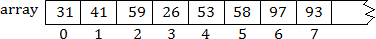
\includegraphics{array_8.png}
\end{figure}

如果把这个有8个元素的数组分成2个有4个元素的数组,然后对每一个子数组排序。记住,应用递归信任可以假定递归调用能正确运行,这样将得到如下结果:
\begin{figure}[!h]
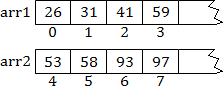
\includegraphics{array_1_2.png}
\end{figure}
这样做的目的是把这些值从子数组中取出来,并以正确顺序放回原数组:
\begin{figure}[!h]
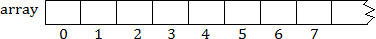
\includegraphics{array_8_1.png}
\end{figure}

\section{合并两个数组}

把已排序的子数组重组成一个完整数组比排序本身要简单,这种技术叫合并(merging)。它基于一个事实,即完整的排序的第一个元素只能是arr1或arr2的第一个元素,但要取更小的那个元素作为第一个元素。

在这个例子中,新数组中的第一个元素是arr1中的26。如果把这个元素放入array[0],实际上,就是把它从arr1中划掉,结果得到以下结构:
\begin{figure}[!h]
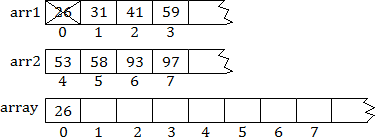
\includegraphics{arr1_arr2.png}
\end{figure}
接着,下一个元素只能是两个子数组中第一个未用过的元素。把arr1中的31和arr2中的53比较,并选择前者:
\begin{figure}[!h]
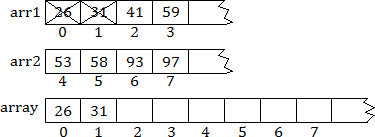
\includegraphics{arr1_arr2_1.png}
\end{figure}
可以继续在arr1、arr2中选择较小值的过程,直到整个数组被填满为止。

\section{合并排序算法}

合并操作与递归分解相结合,产生了一个新的排序算法——合并排序(merge sort),实现这个算法的方法很简单。函数SortIntegerArray首先判定数组的大小。如果数组没有元素或只有一个元素,那么数组必然已经被排过序。因此这个条件定义了这种简单情况。然而,如果数组包含的元素多于1个,就需要执行下列步骤:

(1)把数组分成两个较小的子数组,每一个数组的大小是原数组的一半。

(2)递归调用SortIntegerArray为每一个小数组排序。

(3)合并两个小数组,写回原数组。

函数SortIntegerArray本身的代码如下:
\begin{verbatim}
void SortIntegerArray(int array[], int n)
{
    int i, n1, n2;
    int *arr1, *arr2;
    if(n > 1){
        n1 = n / 2;
        n2 = n – n1;
        arr1 = NewArray(n1, int);
        arr2 = NewArray(n2, int);
        for(i = 0; i < n1; i ++) arr1[i] = array[i];
        for(i = 0; i <n2; i ++) arr2[i] = array[n1 + i];
        SortIntegerArray(arr1, n1);
        SortIntegerArray(arr2, n2);
        Merge(array, arr1, n1, arr2, n2);
        FreeBlock(arr1);
        FreeBlock(arr2);
    }
}
\end{verbatim}
在这个实现中,arr1和arr2是较小的数组,它们有效长度分别为n1和n2,所有困难的工作都由Merge完成,Merge实现如下:
\begin{verbatim}
static void Merge(int array[], int arr1[], int n1, int arr2[], int n2)
{
    int p, p1, p2;
    p = p1 = p2 = 0;
    while(p1 < n1 && p2 < n2){
        if(arr1[p1] < arr2[p2]){
            array[p ++] = arr1[p1 ++];
        }else{
            array[p ++] = arr2[p2 ++];
        }
    }
    while(p1 < n1) array[p ++] = arr1[p1 ++];
        while(p2 < n2) array[p ++] = arr2[p2 ++];
}
\end{verbatim}
Merge函数的参数有目标数组以及较小的数组arr1和arr2,还有它们的有效长度n1和n2。

下标p1和p2标志着每一个子数组的进度,p是array的下标。在每一个循环周期中,函数从arr1或arr2中选择一个较小元素,把该值复制到array中。一旦任何一个子数组的元素用完,该函数就直接把另一个子数组中剩下的元素复制到目标数组中,不用再进行比较测试了。实际上,因为知道当第一个while循环结束时,有一个子数组已经为“空”,所以函数把另一个数组剩下的部分复制到目标位置即可。一个子数组为空后,则相应的while循环将不用执行。

\section{合并排序的计算复杂性}

下面讨论通过函数SortIntegerArray实现分而治之的策略时的效率,虽然可以通过为数组排序并计时来测量其效率,但是从考虑计算复杂性着手会更有帮助。

当调用合并排序的实现(SortIntegerArray函数)为N个数字排序时,运行时间可分成下面两部分:

(1)在当前的递归分解层次上,执行操作所需的所有时间。

(2)执行递归调用的时间。

在递归分解的最上面一层,执行非递归操作所消耗的时间与N成正比。SortIntegerArray的两个for循环一起形成N个循环周期,对Merge的调用填满了原数组的N个位置。如果把这些操作加起来,去掉常量因子,会发现任何一次SortIntegerArray调用的复杂性(如果不考虑其中的递归调用)需要O(N)次操作。

但是递归操作的代价又如何呢?要排序一个大小为N的数组,必须递归地排序两个大小为N / 2的数组。为每一个子数组排序都需要同样的时间。如果应用同样的逻辑,则很快就能够确定每一个递归调用需要的时间正比于该层上的N / 2,加上递归调用所需时间。继续同样的过程,直到到达一种简单情况,即子数组只有一个元素或无元素为止。

解决这个问题所需的总时间是递归分解的每一层所消耗的时间之和。总的来说,分解的结构如下图所示。
\begin{figure}[!h]
\centering
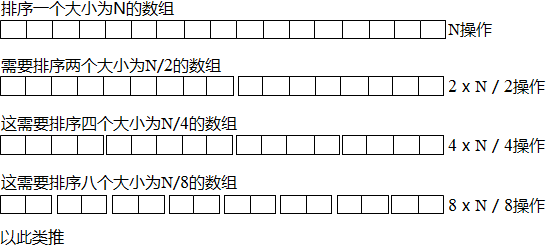
\includegraphics[height=120pt,keepaspectratio]{sort_merge.png}
\caption{合并排序的递归分解}
\end{figure}
当沿着递归层次向下执行时,数组越来越小,但数组个数却越来越多。然而,每一层的工作量总是和N直接成正比的。因此,确定工作总量就转化为确定层数的问题。

在递归层次结构的每一层中,$N$值都除以2。总层数等于你在$N=1$之前将州除以2的次数。

用数学术语表述这个问题,就是说必须找到一个这样的k值,使得
\[N=2^k\]
解这个方程,得到k的值为:
\[k=\log_2^N\]
因为层数为$\log_2^N$,且每一层的工作量与N成正比,所以总工作量与$Nlog_2^N$成正比。

在其他学科中,对数的底数通常为10(常用对数)或数学常量e(自然对数),但在计算机科学中,总是使用二进制对数(binary~logarithm),即以2为底数的对数。由于对数计算底数不同,而底数又是常数,因此,当谈到计算复杂性的问题时,可以像以前那样忽略对数的底数。这样合并排序的计算复杂性可以写为:
\[O(N\log N)\]

\section{比较平方复杂性与NlogN复杂性的性能}

至于$O(N\log N)$的性能到底有多好,可以把它和$O(N^2)$作比较。对于不同的$N$值,这两个函数的值如下表所示。
\begin{table}[!h]
\centering
\caption{ $N^2$和$N\log N$的比较}
\begin{tabular}{|l|l|l|}
\hline
$N$				& $N^2$			&  $N\log N$		\\
\hline
10					& 100				& 33				\\
\hline
100 				& 10~000		& 664				\\
\hline
1~000				& 1~000~000	& 9~965			\\
\hline
10~000			& 100~000~000& 132~877		\\
\hline
\end{tabular}
\end{table}

在这个表中,随$N$值变大,两个列中的数值也增大,但$N^2$一栏增大的速度比$N\log N$栏增大得快,因此基于$N\log N$算法的排序策略能够更广泛地应用于各种大小的数组。

为了在实践中证实上表中的理论结果,因为大$O$标记消去了所有的常量,所以选择排序可能对于有某种规模的问题来说更有效。对不同大小的数组分别运行选择排序和合并排序,并测量实际运行时间,得到下表中的结果。因为计算机的速度有所不同,这些数值可能随机器的不同而有所变化,但基本的模式应该是一样的。
\begin{table}[!h]
\centering
\caption{排序算法的运行时间(以秒为单位)}
\begin{tabular}{|l|l|l|}
\hline
$N$			& 选择排序				& 合并排序			\\
\hline
10 				& 0.000~13				& 0.000~94			\\
\hline
100 			& 0.009~67				& 0.012				\\
\hline
1~000 		& 1.08					& 0.14				\\
\hline
10~000		& 110.0					& 1.6					\\
\hline
\end{tabular}
\end{table}

对于有10个元素的数组来说,选择排序比合并排序快4倍。对于有100个元素的数组来说,选择排序还是较快,但只快一点点。但当达到10~000个元素时,选择排序比合并排序慢70倍,需要将近2分钟来完成。

这些增长系数正是我们想从计算复杂性中得到的。在将数组大小乘以10时,选择排序所需时间应增加100倍,而表中数据验证了这一点。对于合并排序,将数组大小增大10倍,将使运行时间增加为原来的10倍多一点,在表中的数据同样可以观察到这个结果。

总结:

$O(1)$叫做有界时间,即工作量是个常数,不受问题大小的影响。给具有$N$个元素的数组中的第$i$个元素赋值,复杂度是$O(1)$,因为可以通过索引直接访问数组中的元素。虽然有界时间通常又叫做固定时间,但工作量却不必一定是固定的,它只是有一个常量界限而已。

$O(\log_2^N)$叫做对数时间,即工作量是问题大小的对数。每次都把问题的数据量减少一半的算法通常都属于这个类别。用二分检索法在有序列表中查找一个值,复杂度就是$O(\log_2^N)$。

$O(N)$叫做线性时间,即工作量是一个常数乘以问题的大小。输出具有$N$个元素的列表中的所有元素,复杂度是$O(N)$。在无序列表中检索一个值的复杂度也是$O(N)$,因为必须检索列表中的每一个元素。

$O(N\log_2^N)$叫做$N\log_2^N$时间,这类算法通常要应用$N$次对数算法。比较好的排序算法(如快速排序、堆排序和合并排序)的复杂度都是$N\log_2^N$。也就是说,这些算法能用$O(N\log_2^N)$的时间把一个无序列表转换成有序列表,不过快速排序算法对于某些输入数据的时间复杂度是$O(N^2)$。

$O(N^2)$叫做二次时间,这类算法通常要应用$N$次线性算法。大多数简单排序算法的时间复杂度都是$O(N^2)$。

$O(2^N)$叫做指数时间,这类算法非常耗时。在下表中可以看到,随着$N$的增长,指数时间增长得非常快。在棋盘中的每一格放稻谷的例子就是指数时间算法,在这个例子中,问题的大小就是稻谷的颗粒数。(还要注意的是,最后一列的值增长得非常快,以至于这个数量级的问题所需的计算时间超出了预计的宇宙生命期限。)

\begin{table}[!h]
\centering
\caption{增长率的对比}
\begin{tabular}{|p{25pt}|p{25pt}|p{25pt}|p{25pt}|p{40pt}|p{160pt}|}
\hline
$N$	&	$\log_2^N$	& $Nlog_2^N$	& $N^2$	& $N^3$	& $2^N$	\\
\hline
1		& 	0				& 1				& 1		& 1		& 2		\\
\hline
2		& 1				& 2				& 4		& 8		& 4		\\
\hline
4		& 2				& 8				& 16		& 64		& 16		\\
\hline
8		& 3				& 24				& 64		& 512		& 256		\\
\hline
16		& 4				& 64				& 256		& 4096	& 65536	\\
\hline
2		& 5				& 160				& 1024	& 32768	& 4294967296\\
\hline
64		& 6				& 384				& 4096	& 262144& 在超级计算机上约为5年\\
\hline
128	& 7				& 896				& 16384	& 2097152& 以纳秒计约为宇宙年龄的600000倍(估计为60亿年)\\
\hline
256	& 8				& 2048			& 65536	& 16777216	& $-$			\\
\hline
\end{tabular}
\end{table}

$O(n!)$叫做阶乘时间。这类算法甚至比指数时间的算法更耗时。货郎担这个图论问题就是一个阶乘时间算法。

\section{多项式时间算法}

数量级是问题大小的多项式的算法叫做多项式时间算法(polynomial-time~algorithms)。多项式是两个或多个代数项的和,每个代数项是一个常量乘以一个或多个变量的非负整数次幂。因此,多项式算法就是数量级(或复杂度)能够用问题大小的幂表示的算法。算法的大$O$符号是多项式中的最高次幂。所有的多项式时间算法都被定义为$P$类(class~P)算法。

把常见的复杂度量级看作一个箱子,我们可以以此对算法复杂度排序。如下图所示:

\begin{figure}[!h]
\centering
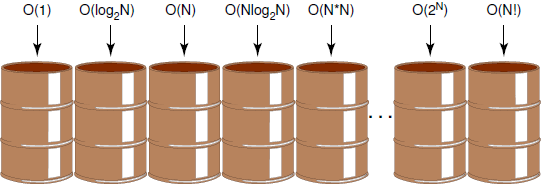
\includegraphics[height=100pt,keepaspectratio]{class_p_box.png}
\caption{复杂度的顺序}
\end{figure}

对于较小的问题,一个箱子中的算法可能真的比下一个更有效的箱子中的等价算法快。随着问题增大,不同箱子中的算法之间的差别会随之增加。在选择同一个箱子中的算法时,就不能再忽略金鱼了。


\section{算法分类}

可以引入箱子的形状来表示常见的算法的数量级,而事实上最右边还应该有一个箱子,存放的是不能解决的算法。

下面将重组这些箱子,把所有多项式算法放在$P$类箱子中,把指数和阶乘算法放在一个箱子中,再加一个不能解决的算法的箱子,如下图所示:

\begin{figure}[htbp]
\centering
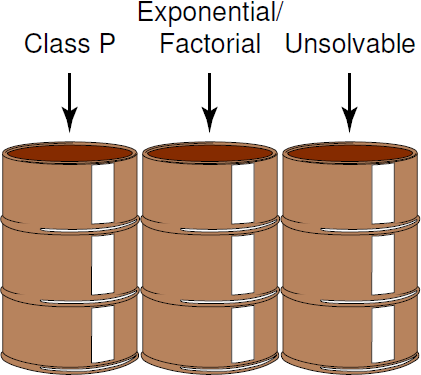
\includegraphics{p_class_box_1.png}
\caption{重组的算法分类}
\end{figure}

在重组后的算法分类中,虽然中间箱子中的算法是有解决方案的,但由于无论数据量大小,它们都要执行很长的时间,所以它们被称为{\heiti 难处理的算法。}

并行计算机体系结构出现以后,如果同时使用足够多的处理器,某些问题就有可能在合理的时间(多项式时间)得到解决了。因此,如果使用足够多个处理器,就能在多项式时间内解决的问题叫做$NP$类问题(Class~NP~problems)。相应地,用一个处理器能在多项式时间内解决的问题叫做$P$类问题(Class~P~problems)。

显然,$P$类问题也是$NP$类问题。理论计算学中的一个未决问题是,只有用多个处理器才能解决的$NP$类问题是否也是$P$类问题。也就是说,这些问题是否存在多项式算法,而目前我们还未发现(发明)。我们不知道这个答案,计算机科学的理论研究这一直在寻求这些的解决方案。

仅仅是判断$P$类是否等价于$NP$类的问题已经被简化为找到其中一个算法的解决方案。有一类的特殊的问题叫做$NP$完全问题(NP-complete~problems)。这些问题属于$NP$类,它们的属性可以互相映射。如果找到了这个类中的一个算法的单处理器多项式时间解决方案,那么其他所有算法都会存在这样的解决方案,因为一个解决方案可以映射到其他所有问题的解决方案。

在我们对复杂度的陈述中加入了新的$NP$类复杂度箱子后,这个箱子和P类箱子相邻的一边用虚线标示了出来,因为它们实际上是一个箱子,算法分类变成如下图所示:

\begin{figure}[htbp]
\centering
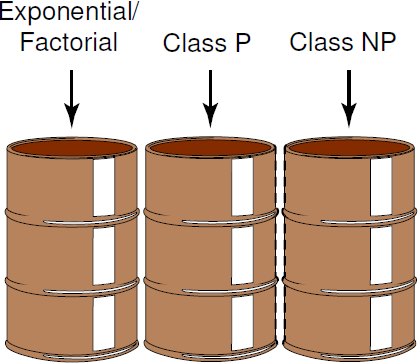
\includegraphics{np_class_box.png}
\caption{加入了NP类}
\end{figure}



\section{货郎担问题}

一个经典的$NP$类问题叫做货郎担问题。一个货郎要走访他的销售区域内的所有城市。为了有效地走访每个城市,他想找到一条路线,在返回起点之前,要经过且只经过每个城市一次。可以用图的顶点表示城市,图的边表示城市间的路。每条边上标有城市之间的距离。这个解决方案成了著名的图论算法,它的单处理器解决方案的复杂度是$O(n!)$。

\chapter{图灵机}

Alan~Turing在20世纪30年代开发了计算机器的概念,他的兴趣并非实现这台机器,而是用它作为一种模型来研究计算的限度。图灵机就是一种抽象数学模型,本质上它与硬件毫无关系。图灵机为计算理论的主要领域奠定了基础,现在分析图灵机的功能是所有学习计算机科学的学生的理论学习的一部分。

Turing所做的就是构想一台假想机,这是一台类似于打字机的简单装置,能够扫描或读取一条理论上无限长的带子上的指令。这台扫描器从带子上的一个方格移到下一个方格,响应序列的指令,并修改它的机械响应,Turing证明了这种过程的输出可以复制人类的逻辑思维。

\begin{figure}[htbp]
\centering
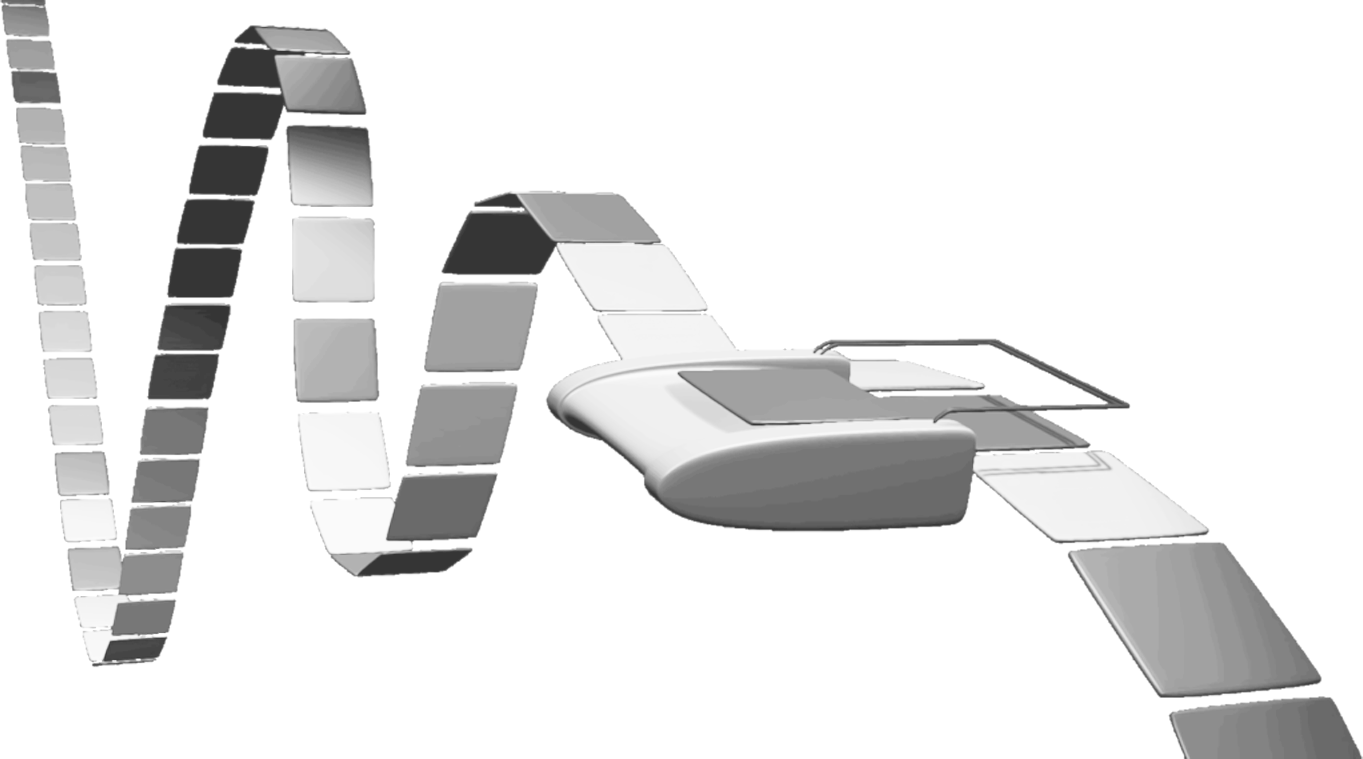
\includegraphics[height=100pt,keepaspectratio]{alan_turing.png}
\end{figure}

这种假想的装置的名字就是——图灵机,Turing的另一个构想也是如此。由于机器的行为是由带子上的指令控制的,改变这些指令,就可以使这台机器执行各种功能。换句话说,采用不同的带子,同一台机器既可以执行运算,又可以下棋,还可以执行其他所有具有计算性的任务,因此这个装置得到了一个新的名字——通用图灵机。

现代计算机的诞生汇集了无数的构想和高级技术,很难把它的发明归功于某个人。不过,每个在使用计算机的人,都在使用具体化了的图灵机。

图灵机由具有读写头的控制部件构成,能够在无限的带子上读写符号,带子被分成了单元。图灵机的基础是一个人用铅笔和橡皮在长长的纸带上进行简单的运算,纸上的每一行(一个单元)包含一个有限字符集中的符号。从第一行开始,这个人分析其中的符号,或者保留它,或者用字符集中的另一个字符替换它。然后他移到下一行,重复上述操作。

图灵机的控制部件模拟了这个人。人的决策过程由控制部件能执行的一系列指令表示。每个指令可以:
\begin{compactitem}
\item 从带子上的一个单元读取一个符号;
\item 把一个符号写入带子上的一个单元;
\item 使带子向左移动一个单元,或向右移动一个单元,或者保持不动。
\end{compactitem}

如果我们允许一个自己替换符号,这些动作其实是模拟了一个使用铅笔的人。

为什么这样一个简单的机器(模型)这么重要呢?一个广为接受的说法是任何能直观计算的问题都能被图灵机计算。这个说法叫做Church-Turing理论,以Turing和Alonzo Church的名字命名,后者开发了另一个类似的模型——$\lambda$演算。

从Church-Turing理论我们可以得出这样的结论,如果证明了一个问题的图灵机解决方案不存在,那么这个问题就是不可解决的。


\chapter{停机问题}

计算(程序)终止并不总是很明显的。比如不同的循环类型中,有些循环会明显地终止,而有的则不会(无限循环),还有些循环是根据输入的数据或循环中发生的计算终止的。在一个程序运行的过程中,很难分辨它是进入了无限循环还是需要更多时间来运行。

因此,如果可以预言一个具有特定输入的程序不会落入无限循环,是非常有用的。停机问题(halting~problem)以下面的方式重新阐述了这个问题,即\verb|给定一个程序和它的输入,确定该程序采用这样的输入最终是否能停止|。

最明显的方法是用特定的输入运行程序,看会发生什么情况。如果它停止了,答案是显而易见。如果它不停止呢?一个程序要运行多久才能判定它落入了无限循环?显然,这种方法有问题。遗憾的是,其他的方法也都有问题。这个问题是不可解决的。这个断言的证明是“没有图灵机程序可以确定一个程序是否在指定的输入下会停止。”

那么如何证明一个问题是不可解决的,或者只是我们还没找到解决方案而已呢?可以尝试每种提出的解决方案,证明每种方法都有问题。由于已知的解决方案可能很多,而且还有很多是未知的,所以这种方法看来行不通。然而这种方法构成了图灵解决方案的基础。在这个证明中,就是从提出的解决方案入手,然后证明它们是行不通的。

假设存在一个图灵程序SolvesHaltingProblem,对于任何程序Example和输入SampleData,它都能确定Example采用SampleData是否会停止。也就是说,程序SolvesHaltingProblem以程序Example和输入SampleData作为参数,如果Example能停止,则输出“Halts”,如果Example具有无限循环,就输出“Loops”。下图展示了这种情况:

\begin{figure}[!h]
\centering
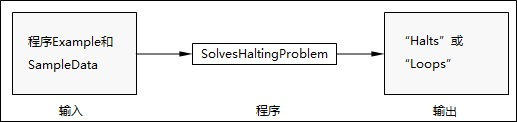
\includegraphics[scale=1.75]{halting_problem_program.png}
\caption{为解决停机问题提出的程序}
\end{figure}

在计算机中,程序(指令)和数据是相似的,都是位组合。程序和数据的区别在于控制部件如何解释位组合。因此,如果把Example自身作为SampleData,那么SolvesHaltingProblem就要以Example程序和它的副本作为参数,来判断Example以其自身作为输入是否会停止。如下图所示:

\begin{figure}[!h]
\centering
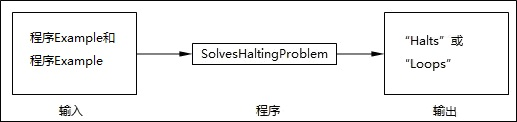
\includegraphics[scale=1.75]{halting_problem_program1.png}
\caption{为解决停机问题提出的程序}
\end{figure}

现在我们构造一个新程序NewProgram,以Example作为程序和输入数据,采用SolvesHaltingProblem的算法,如果Example会停止,就输出“Halts”,如果Example具有无限循环,就输出“Loops”。如果输出了“Halts”,NewProgram将创建一个无限循环;如果输出的是“Loops”,NewProgram将输出“Halts”。下图展示了这种情况:

\begin{figure}[!h]
\centering
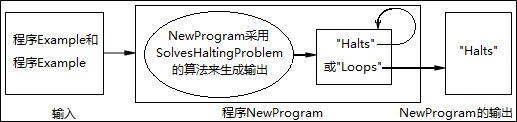
\includegraphics[scale=1.75]{new_halting_problem_program.png}
\caption{NewProgram的构造}
\end{figure}

这个证明就是,把SolvesHaltingProblem应用到NewProgram上,以NewProgram作为输入数据。如果SolvesHaltingProblem输出“Halts”,那么NewProgram就落入了无限循环。如果SolvesHaltingProblem输出“Loops”,NewProgram将输出“Halts”并停止。无论哪种情况,SolvesHaltingProblem所给答案都是错的。由于SolvesHaltingProblem至少会对一种情况给出错误答案,所以它不适用于所有情况。因此,任何提出的解决方案都是有问题的。

\clearpage
\bibliography{csnotes}
\bibliographystyle{plainnat}
























\include{Glossary_of_Terms}


\end{document}

